\frontmatter

%!TEX root = forallxyyc.tex

% Bastard Title

\pagestyle{empty}

\vspace*{80pt}

\begin{raggedleft}
\fontsize{30pt}{24pt}\sffamily
\selectfont
  \textbf{forall 
  {\fontsize{37pt}{24pt}\selectfont\rmfamily\textit{x}}: 
  $R^3$}

\medskip\fontsize{18pt}{20pt}\selectfont

\textbf{A Remixed, Revised, and Reimagined\\Introduction to\\ Formal Logic}

\vfill
\fontsize{12pt}{16pt}\selectfont \textit{By }  \textbf{Davis A. Smith}\\
     \textit{based on the related works by}\\
      \textbf{P.~D. Magnus}\\
      \textbf{Tim Button}\\
%      \textit{with additions by}\\
      \textbf{J.~Robert Loftis}\\
      \textbf{Robert Trueman}\\
      \textbf{Aaron Thomas-Bolduc}\\
      \textbf{Richard Zach}\par


\vfill
\textbf{\forallxversion}\par
\end{raggedleft}


\newpage


\noindent\small%
\forallx: \emph{$R^3$} by Davis A. Smith is a revision and expansion of \href{https://forallx.openlogicproject.org/}{\forallx: \emph{Calgary}}, 
by Aaron Thomas-Bolduc and Richard Zach, used under a 
\href{https://creativecommons.org/licenses/by/4.0/}{CC BY 4.0} license, which was based on
\href{https://www.homepages.ucl.ac.uk/~uctytbu/OERs.html}{\forallx:
\emph{Cambridge}}, by 
\href{https://www.homepages.ucl.ac.uk/~uctytbu/}{Tim Button} (University College London), 
used under a \href{https://creativecommons.org/licenses/by/4.0/}{CC BY
4.0} license, which was based, in turn,
on \href{https://www.fecundity.com/logic/}{\forallx}, by
\href{https://www.fecundity.com/job/}{P.D.\ Magnus} 
(University at Albany, State University of New York),
used under a \href{https://creativecommons.org/licenses/by/4.0/}{CC BY
4.0} license.
It includes additional material from \forallx{} by P.D. Magnus and
\href{https://www.homepages.ucl.ac.uk/~uctytbu/OERs.html}{\emph{Metatheory}} by Tim Button, 
used under a \href{https://creativecommons.org/licenses/by/4.0/}{CC BY
4.0} license, and 
from \href{https://github.com/rob-helpy-chalk/openintroduction}{\forallx: \emph{Lorain
County Remix}},
by \href{https://sites.google.com/site/cathalwoods/}{Cathal Woods} and
J. Robert Loftis as well as original material by Davis A. Smith. Biographies for Alan Turing, Bertrand Russell, and Kurt G\"{o}del were provided by \href{https://builds.openlogicproject.org/}{The Open Logic Project} and used under a \href{https://creativecommons.org/licenses/by/4.0/}{CC BY 4.0} license. The biography for William of Ockham was provided by \href{https://sites.google.com/view/andrewjefferyswebpage}{Andrew Jeffery} and used with his permission. The image used in the biography of William of Ockham was taken by \href{https://www.geograph.org.uk/profile/9419}{John Salmon} and used under a \href{https://creativecommons.org/licenses/by-sa/2.0/}{CC BY 2.0} license. 

\bigskip

\noindent \footnotesize This work is licensed under a \href{https://creativecommons.org/licenses/by/4.0/}{Creative Commons Attribution 4.0} license.
You are free to copy and redistribute the material in any medium or format, and  remix, transform, and build upon the material for any purpose, even commercially, under the following terms:
\begin{itemize}
\item You must give appropriate credit, provide a link to the license, and indicate if changes were made. You may do so in any reasonable manner, but not in any way that suggests the licensor endorses you or your use.
\item You may not apply legal terms or technological measures that legally restrict others from doing anything the license permits.
\end{itemize}

\bigskip
\noindent Cover design by Mark Lyall.

\clearpage
\pagestyle{leadbeater}
\thispagestyle{plain}
\currentpdfbookmark{Table of Contents}{name}
\tableofcontents*

\chapter{Preface}

This textbook concerns formal logic. Formal logic, as a field, is a subdiscipline within Philosophy which studies the relationship between assumptions (premises) and conclusions. It is `formal' in the sense that it concerns the \emph{form} or \emph{shape} of the assumptions/conclusions on an abstract level so the same logical structure can be used in many different unrelated contexts with the same level of certainty. The forms of these arguments are expressed through the use of \emph{formal languages}, namely Propositional Logic, Quantified Logic, and Modal Logics. Being formal, these languages are very useful in that it is impossible to be ambiguous. The study of such formal languages centers on entailment, that is, what follows from what; by better understanding entailment, we can better tell what will be a necessary consequence of a state of affairs or situation. We can, in a sense, predict the future. Studying these formal languages also gives us a better understanding of notions like possibility, necessity, validity, and soundness. Formal languages naturally have the ability to precisely define these notions using either the basic aspects of the language or the systems of deduction which the language naturally provides.

The importance of formal logic and these formal languages extends beyond Philosophy and regular reasoning/argumentation into other fields such as Mathematics and Computer Science. In Mathematics, formal languages are used to describe mathematical situations rather than normal ``everyday'' ones. For their proofs and discoveries, mathematicians are fundamentally interested in the consequences of definitions and assumptions and it is very important for them to establish these consequences (which they call ``theorems'') using extremely precise and rigorous methods so that they will hold regardless of the circumstances. Formal logic provides those methods. 

In computer science, formal logic is applied to describe the state and behaviours of computational systems, e.g., circuits, programs, databases, and the like. The methods in formal logic are used to establish whether a circuit is error-free, such as whether it returns the correct output given some set of inputs; whether a program does what it's intended to do; whether the structure of a database is consistent, whether the storage of the data is optimally compact, or if something is true of the data in it; and other areas of concern. In fact, the underlying frameworks for computer programming languages are based on the formal languages in formal logic. 

The book is divided into ten (10) modules. Module~\ref{ch.intro} introduces the topic and notions of logic in an informal way, without introducing a formal language yet.  Modules \ref{ch.symbolizing}--\ref{ch.plnd2} concern truth-functional languages. In it, sentences are formed from basic sentences using a number of connectives (`or', `and', `not', `if \dots then') which combine sentences into more complicated ones.  We discuss logical notions such as entailment in two ways: semantically, using the method of truth tables (in Module~\ref{ch.TruthTables}) and proof-theoretically, using a system of formal derivations (in Modules~\ref{ch.plnd1}--\ref{ch.plnd2}).  Modules \ref{ch.qlsymbolizing}--\ref{ch.qlnd2} deal with a more complicated language, that of first-order logic, called Quantified Logic. It includes, in addition to the connectives of truth-functional logic (called Propositional Logic), also names, predicates, identity, and quantifiers. These additional elements of the language make it much more expressive than Propositional Logic and able to handle far more complicated situations. We'll spend a fair amount of time investigating just how much one can express in it.  Again, logical notions for Quantified Logic are defined semantically, using interpretations, and proof-theoretically, using a more complex formal derivation system introduced in Modules \ref{ch.qlnd1} and \ref{ch.qlnd2}.  Module~\ref{ch.ml1} discusses the extension of PL by non-truth-functional operators for possibility and necessity: modal logic. In the appendices you'll find proofs concerning metalogical concepts such as \emph{soundness} and \emph{completeness}, a chapter outlining the link between computer circuits and Propositional Logic, a quick reference listing the rules and restrictions (if necessary) for the truth conditions and inference rules, and a glossary listing central terms used thoughout the book. Future editions of this book will include content and proof-systems for deviant logics, such as paraconsistent logic and other many-valued logics, content and proof-systems for alternative applications of Modal Logic (such as Temporal, Deontic, and Epistemic Logics), and a more in depth exploration of inductive reasoning and informal fallacies. 

\paragraph{Credits} This book is based on \forallx: \emph{Calgary}, by Aaron Thomas-Bolduc and Richard Zach which was based on a text originally written by P.~D. Magnus in the version revised and expanded by Tim Button. Through \forallx: \emph{Calgary}, it also includes some material by J.~Robert Loftis and some material by Robert Trueman (mostly content in Module~\ref{ch.ml1}). Davis A. Smith `remixed' and revised the material provided by Aaron Thomas-Bolduc and Richard Zach and then expanded upon it with his own original content, including but not limited to: Redefining an inference rule, adding a new equivalency rule, including more examples, reimagining the proof system for the Modal Logics (adding new inference rules and redesigning the `strict subproof' system for better implementation into Carnap.io), adding biographies for various prominate logicians, metalogical proofs for soundness and completeness, and a chapter outlining the connection between formal logic and computer circuits (logic gates). The biography for William of Ockham was provided by Andrew Jeffery and used with his permission. The resulting text is licensed under a Creative Commons Attribution 4.0 license. There are \href{https://github.com/OpenLogicProject/OpenLogic/wiki/Other-Logic-Textbooks}{several other} ``remixes'' of \emph{forall x} available freely online.

\paragraph{Notes for instructors} This book was designed for a quarter-long (10 weeks) introduction to formal logic. In my classes, I (Davis A. Smith) cover all modules, spending 1 week per module. 
The CC BY license gives you the right to download and distribute the book yourself. In order to ensure that all your students have the same version of the book throughout the term you're using it, you should upload the PDF you decide to use to your LMS rather than merely give your students a link to the source. You are also free to have the PDFs printed by your bookstore.

The syntax and proof systems are supported by Graham Leach-Krouse's free, online logic teaching software application \href{https://carnap.io}{Carnap.io}. I recommend that this be included in your course as a course companion. It allows for submission and automated marking of exercises such as symbolization, truth tables, and natural deduction proofs.

\mainmatter
\setsecnumdepth{part}
%!TEX root = forallxd.tex
\part{Arguments and Logic}
\label{ch.intro}
\addtocontents{toc}{\protect\mbox{}\protect\hrulefill\par}


\chapter{Part 1: Arguments and Propositions}
\section{Part 1.1: Arguments: What is logic?}
\label{s:Part 1.1: Arguments: What is logic?}

The common-sense, everyday, way to tell whether a claim is true or false is to look at the reasons for or against it. Sometimes our observations give us good reasons. For example, I have a good reason for thinking my bicycle has a flat tire when I see the tire sagging on the rim or hear air hissing out of the tube. But often the business of identifying and evaluating reasons is a bit more involved. Logic is the business of identifying and evaluating reasons. You do this all the time. You give yourself reasons to choose one shirt over another for a job interview, you reason your way through making a choice about which classes to take, you believe certain things based on evidence, and you give reasons for why something isn't your fault (when you make excuses). In all of these cases and more, you are making \glspl{argument}.

This is very different from how you might use the term ‘argument'. In everyday language, we sometimes use the word ‘argument’ to talk about belligerent shouting matches. If you and a friend have an argument in this sense, things are not going well between the two of you. Logic is not concerned with such teeth-gnashing and hair-pulling. They are not arguments, in our sense; they are just disagreements. For a humorous example of how arguments and disagreements differ, take a look at this funny exchange from Monty Python:\autocite{ArgumentClinic}

\factoidbox{\begin{multicols}{2}
Man: Is this the right room for an argument?\\
Other Man:(John Cleese) I've told you once.\\
Man: No you haven't.\\
Other Man: Yes I have.\\
M: When?\\
O: Just now.\\
M: No you didn't!\\
O: Yes I did!\\
M: You didn't!
\ldots\\
O: Oh I'm sorry, is this a five minute argument, or the full half hour?\\
M: Ah! (taking out his wallet and paying) Just the five minutes.\\
O: Just the five minutes. Thank you.\\
O: Anyway, I did.\\
M: You most certainly did not!\\
O: Now let's get one thing quite clear: I most definitely told you!\\
M: Oh no you didn't!\\
O: Oh yes I did!
\ldots\\
M: Oh look, this isn't an argument!\\
(pause)\\
O: Yes it is!\\
M: No it isn't!\\
(pause)\\
M: It's just contradiction!\\
O: No it isn't!\\
M: It IS!\\
O: It is NOT!
\ldots\\
M: (exasperated) Oh, this is futile!!\\
(pause)\\
O: No it isn't!\\
M: Yes it is!\\
(pause)\\
M: I came here for a good argument!\\
O: AH, no you didn't, you came here for an argument!\\
M: An argument isn't just contradiction.\\
O: Well! it CAN be!\\
M: No it can't!\\
M: \emph{An argument is a connected series of statements intended to establish a proposition.}\\
O: No it isn't!\\
M: Yes it is! ‘tisn't just contradiction.\\
O: Look, if I \emph{argue} with you, I must take up a contrary position!\\
M: Yes but it isn't just saying ‘no it isn't'.\\
O: Yes it is!
\ldots\\
M: No it ISN'T! \emph{Argument is an intellectual process.} Contradiction is just the automatic gainsaying of anything the other person says.\\
O: It is NOT!\\
M: It is!
\ldots 
\end{multicols}}

An argument is a reason for taking something to be true. \Glspl{argument} are made out of two or more claims, one of which is a \gls{conclusion}. The conclusion is the claim the argument purports to give a reason for believing. The other claims are the \glspl{premise}. The premises of an argument taken together are offered as a reason for believing its conclusion. In the above exchange, the person looking for an argument claims that "An argument is a collected series of statements to establish a definite proposition". This is a close approximation to how philosophers use the term, but a better, more exact definition is:
\begin{center}
An argument is a collected series of propositions intended to establish others in the series.
\end{center}
We will be returning to what, exactly, propositions are in a moment but the propositions (statements, in this case) which support others are our premises. The one being supported is the conclusion.  This is very different from a disagreement; in the above discussion, the contrarian (‘O') is conflating disagreement with argument.  A disagreement is where you have two things (often people) which do not agree about the truth of some proposition.  Often, in at least a reasonable disagreement, one or both of the parties will give arguments in support of their side. They will give reasons for why they are correct and the opposing side is, thereby, wrong. So, an argument, as we will understand it, is something more like this:
	\begin{earg}\label{argButlerGardner}
		\item[] Either the butler or the gardener did it.
		\item[] The butler didn't do it.
		\item[\therefore] The gardener did it.
	\end{earg}
We here have a series of sentences. The three dots on the third line, \gls{therefore}, of the argument are read ‘therefore.’ They indicate that the final sentence expresses the conclusion of the argument. The two sentences before that are the premises of the argument. If you believe the premises and you think the conclusion follows from the premises (that the argument, as we will say, is valid), then this (perhaps) provides you with a reason to believe the conclusion.

This is the sort of thing that logicians are interested in.  Without arguments, we would be unable to tell which side is correct. In fact, without arguments, we wouldn't be able to decide anything (all of our choices would be completely random). We will say that an argument is any collection of premises, together with a conclusion. 

Logic, as a discipline, is the study of arguments and structures of reasoning. In this class, you will learn and apply various simple reasoning structures (called ‘rules of inference') and learn to identify when two statements mean the same thing and how to move between these statements.

\newglossaryentry{therefore}{
name = {\therefore},
text = \therefore,
description = {A shorthand for the various ways in ordinary language we indicate the conclusion to an argument or line of reasoning, \gls{conclusion indicator word}s}
} 

\subsection{What are we doing in this first module?}

This first module discusses some basic logical notions that apply to arguments in a natural language like English (these same principles apply to all natural languages and to many artificial languages (sometimes called ‘Conlangs' for constructed languages)). It is important to begin with a clear understanding of what arguments are and of what it means for an argument to be valid. Later (in Module \ref{ch.symbolizing}), we will translate arguments from English into a formal language. This move from a natural language to a formal, logical, one is important. The formal language allows us to look at how the argument was reasoned and avoid the biases we are prone to have when we know what was reasoned.  We want formal validity, as defined in the formal language, to have at least some of the important features of natural-language validity so that it translates over to our every-day life.

\subsection{The general structure of an argument}

In the butler and gardener examples above, we used individual sentences to express both of the argument’s premises, and we used a third sentence to express the argument’s conclusion. Many arguments are expressed in this way, especially when clarity is more important than efficiency or rhetoric, but a single sentence can contain a complete argument. Consider:
	\begin{quote}
		 The butler has an alibi; so they cannot have done it.
	\end{quote}
This argument has one premise followed by a conclusion. There are likely some \glspl{implied premise} such as "if the butler has an alibi, then they cannot have done it". In a formal language, such as the one you will be learning in this class, those will need to be explicit. Many arguments, such as that one,  start with premises, and end with a conclusion, but not all of them. The argument with which this section began might equally have been presented with the conclusion at the beginning, like so:
	\begin{quote}
		The gardener did it. After all, it was either the butler or the
		gardener. And the butler didn't do it.
	\end{quote}
So, in this case, the premises are "it was either the butler or the gardener" and "the butler did it". Here, we don't have, or don't need, any implied premises. Equally, it might have been presented with the conclusion in the middle:
	\begin{quote}
		The butler didn't do it. Accordingly, it was the gardener,
		given that it was either the gardener or the butler.
	\end{quote}
When approaching an argument, we want to know whether or not the conclusion follows from the premises. So the first thing to do is to separate out the conclusion from the premises. As a guide, these words are often used to indicate an argument's conclusion:
	\begin{center}
		so, therefore, hence, thus, accordingly, consequently
	\end{center}
For this reason, they are sometimes called \glspl{conclusion indicator word}. By contrast, these expressions are \glspl{premise indicator word}, as they often indicate that we are dealing with a premise, rather than a conclusion:
	\begin{center}
		since, because, given that
	\end{center}
But in analysing an argument, there is no substitute for a good nose.


\newglossaryentry{implied premise}
{
name=implied premise,
description={A premise of an argument which is not explicitly stated but rather is hinted at or inferred by the context}
}


\section{Part 1.2 Sentences and Propositions}
\label{Some Basics from Philosophy of Language}

To be perfectly general, we can define an \gls{argument} as a series of sentences. The sentences at the beginning of the series are premises. The final sentence in the series is the conclusion. If the premises are true and the argument is a good one, then you have a reason to accept the conclusion.

In logic, we are only interested in sentences that can figure as a premise or conclusion of an argument, i.e., sentences that can be true or false. This helps us avoid the pulls of rhetoric and certain kinds of fallacious reasoning. We also want to make sure that we all have attached the same meaning to a sentence, as to avoid the potential confusion resulting from us talking past each other. So, in general, logic is focused on propositions.

This is where we get into a very basic introduction into Philosophy of Language. This area of philosophy deals with things such as meaning, reference, and so forth (Philosophy of Language is what I mostly work in, it deals with semantics while Linguistics deals with syntax, but the fields overlap quite a bit). Even when we aren't trying very hard, we can use words and sentences in a ton of different ways and there seems to be some vagueness or ambiguity in natural languages. For example, I can easily make examples where sentences might have two or more different interpretations, like double or triple entendres. \\
\begin{earg}
\item[\ex{ambi1}] GOP grills the IRS chief over lost emails.
\item[\ex{ambi2}] If your dog poops, you must put it in the trash can.
\item[\ex{ambi3}] A woman gives birth in the UK every 48 seconds.
\item[\ex{ambi4}] People wanted for pickling and canning.
\end{earg}
All four of the above examples have at least 2 different interpretations and, in each case, one seems true while the other seems false. In Example \ref{ambi1}, it could be interpreted to mean that the GOP are having an IRS chief BBQ over a server or it could mean that they are harshly questioning the chief. In Example \ref{ambi2}, one way to understand this is that it's telling you to put your dog in the garbage can, while another is telling you to put the poop therein. In Example \ref{ambi3}, we could say that there's a single woman who is having a baby every 48 seconds (she must be tired) or that some woman, not necessarily the same woman, is having a child in that time. In Example \ref{ambi4}, it could be that we have a cannibal looking to store their meats for the winter using canning and fermenting techniques or it could be that a food fermentation business is looking to hire on some more people in those departments. Given these examples, and how often we misunderstand each other on a daily basis,  it might be tempting, therefore, to think that the truth of a sentence must be relative to its interpretation.  In an even more robust example, imagine the following:
\factoidbox{Suppose that we all collectively switched the sorts of things the words ‘dog' and ‘cat' pick-out. So, the word ‘dog' now is used to point out the meowing critters and the word ‘cat' refers to the barking ones. In this case, it would seem that the sentence ‘dogs are canines' would be false and ‘dogs are feline' would be true. If we, again, flipped the meanings of the words ‘feline' and ‘canine', we would get that ‘dogs are canines' as true, but for a totally different reason than it was originally.}
But does this make truth open for interpretation? Well, no, but in a sense, yes. When we look at a language, from one perspective, we notice that things like words and sentences are nothing more than characters on a screen/page, random collections of sounds, or certain structured gestures (in the case of sign languages). Those things, on their own, don't have meaning. There must be something extra, beyond the sound and signs, which has the meaning.  Philosophers call the meaning behind a sentence a \gls{proposition}. A proposition, itself, is not a sentence or a word, rather it's the meaning behind the sentences.\\

\newglossaryentry{proposition}
{
name=proposition,
description={The meaning behind a declarative sentence or expression}
}

\begin{center}
\begin{tabular}{c|c|c}\hline
Sentence&Language&Proposition\\\hline
Snow is white&English&that snow is white\\
Schnee ist Weiss&German&that snow is white\\
Nix alba est&Latin&that snow is white\\
La neige est blanche&French&that the snow is white\\
\hline
\end{tabular}
\end{center}
All of the above examples are different sentences, made clear because they are in different languages, but they all express the same proposition. The truth of a sentence is relative to the truth of the proposition attached to it, propositions are the things which are true or false, and then the truth of the proposition is determined by its correspondence with reality. Translators, at least the good ones, often take the sentence in one language, figure out the proposition connected to it, and then express the same proposition in the necessary language.

\subsection{The Move to Propositions}
So, the proposition expressed by a sentence is not itself a linguistic thing. Propositions themselves don't have meaning, but rather they are the meaning behind a sentence. For a bit of language to be open to interpretation is for us to be able to attach different propositions (meanings) to it. But the meanings themselves are not open to further interpretation. And it is the proposition, what is meant by the sentence, which makes the statements, sentences, true or false. So, when I speak of arguments consisting of premises (the supporting evidence and their arrangement in the argument), I am talking about the core meaning behind the sentence, not the sentence itself. If we misinterpret the sentence, then we haven’t yet gotten on to the claim being made and hence probably don’t fully understand the argument.

You should not confuse the idea of a sentence which can express propositions with the difference between fact and opinion. Often, sentences in logic will express things that would count as facts— such as ‘Kierkegaard was a hunchback’ or ‘Kierkegaard liked almonds’ but they can also express things which you might think of as matters of opinion—such as, ‘almonds are tasty.’ In other words, a sentence is not disqualified from being part of an argument because we don’t know if it is true or false or because its truth or falsity is a matter of opinion. If it is the kind of sentence that could be true or false, then it can play the role of premise or conclusion.

Also, there are things that would count as ‘sentences’ in a linguistics or grammar course which do not necessarily express propositions. Here are just a few:

\subsection{Questions} In a grammar class, `Are you sleepy yet?' would count as an interrogative sentence. Although you might be sleepy or you might be alert, the question itself is neither true nor false. For this reason, questions will not count as sentences in logic. Suppose you answer the question: `I am not sleepy.' This is either true or false, and so it is a sentence in the logical sense. Generally, \emph{questions} will not count as sentences, but \emph{answers} will. `What is this course about?' is not a sentence (in our sense). `No one knows what this course is about' is a sentence. 

\subsection{Imperatives} Commands are often phrased as imperatives like `Wake up!', `Sit up straight', and so on. In a grammar class, these would count as imperative sentences. Although it might be good for you to sit up straight or it might not, the command is neither true nor false. Note, however, that commands are not always phrased as imperatives. In the right context, the sentence `you will respect my authority' \emph{is} either true or false---either you will or you will not---and so it counts as a sentence in the logical sense. In another context, however, it is an imperative, so it is not the sort of thing which is true or false. Understanding which is the correct interpretation is essential to understanding language.  

\subsection{Exclamations} `Ouch!' is sometimes called an exclamatory sentence, but it is neither true nor false. We will treat `Ouch, I hurt my toe!' as meaning the same thing as `I hurt my toe.' The `ouch' does not add anything that could be true or false. Certain phrases use words and bits of language which in other contexts would amount to sentences but are in fact exclamations. For example, "you jerk!" could be easily seen as a colloquial shortening of "you are a jerk!" which is something which can be true or false, either the \emph{you} in question is a jerk or they are not. But it could also be seen as an exclamation without any additional content. As before, the context very much matters. 

\practiceproblems
\problempart
\label{pr.IDargs}
For each, identify whether it is an argument, in the logical sense.
\begin{enumerate}
\item Betty and Sue are worried about their son, Max, who is late getting home. Betty thinks that they should get in the car and drive over to his friend's house while Sue thinks that they should give Max a little more time, as he could of lost track of it. 
\item Bernie and Tommy disagree about whether they can afford to go on vacation to the ski slopes in Canada this winter. Bernie says ``Of course we can afford it. After all, you and I are both employed, we have a ton of paid time-off built up, and I have even laid out the budget here.''
\item Jesus loves me, this I know, because the Bible tells me so. 
\item Ashley and Abbott are unsure about who said the famous line ``iacta alea est''. Kirsten chimes in from across the room: ``It was Julius Caesar!''
\item If absence makes the heart grow fonder, then attendance makes the heart grow colder. Obviously, you have been in my presence for too long. 
\item I know. You know I know. I know you know I know. We know Henry knows, and Henry knows we know it. We're a knowledgeable family.
\end{enumerate}

\problempart
\label{pr.IDprops}
For each, identify whether it expresses a proposition. If there are multiple sentences, identify which, if any, express a proposition.
\begin{enumerate}
\item Mom asked me whether I would be home in time for dinner. I replied ``yes.''
\item What time do you want me to pick you up from the mall? 
\item Oh, Freddy, \emph{you} don't think I'm a heartless guttersnipe, do you?
\item A young boy says that he hates spinach. Later he says that he is glad he hates spinach. Why? Because ``if I liked spinach, I would eat it, and it's just gross!''
\item I believe that Julius Caesar crossed the Rubicon.
\item Max is such a jerk. I mean, how could anyone like him? 
\end{enumerate}


\chapter{Part 2: Types of Arguments}
\label{s:Valid}

\section{Part 2.1: Consequence and validity}

In Part 1, we talked about arguments, i.e., a collection of sentences (the premises), followed by a single sentence (the conclusion). We said that some words, such as “therefore,” indicate which sentence is supposed to be the conclusion. “Therefore,” of course, suggests that there is a connection between the premises and the conclusion, namely that the conclusion follows from, or is a consequence of, the premises. This notion of consequence is one of the primary things logic is concerned with. Referencing back, one might even say that logic is the science of what follows from what. Logic develops theories and tools that tell us when a proposition follows from some others. Take, for example, the argument which I used in Part 1:
\begin{earg}
	\item[] Either the butler or the gardener did it.
	\item[] The butler didn't do it.
	\item[\therefore] The gardener did it.
\end{earg}
We don’t have any context for what the sentences in this argument refer to. Perhaps you suspect that “did it” here means “was the perpetrator” of some unspecified crime (we don't necessarily know what the correct proposition is for that sentence in this context because we don't know the context). You might imagine that the argument occurs in a mystery novel or TV show, perhaps spoken by a detective working through the evidence. But even without having any of this information, you probably agree that the argument is a good one because of the basic structure which is used. In this sense, whatever the premises refer to, if they are both true, the conclusion must be true as well. If the first premise is true, i.e., it’s true that “the butler did it or the gardener did it,” then at least one of them “did it,” whatever that means. And if the second premise is true, then the butler did not “do it.” That leaves us with only one option: “the gardener did it” must be true. Here, the conclusion follows from the premises. We call arguments that have this property \gls{valid}.
By way of contrast, consider the following argument:
\begin{earg}\label{argMaidDriver}
	\item[] If the driver did it, the maid didn't do it.
	\item[] The maid didn't do it.
	\item[\therefore] The driver did it.
\end{earg}
We still have no idea what is being talked about here. But, again, you probably agree that this argument is different from the previous one in an important respect. If the premises are true, it is not guaranteed that the conclusion is also true. (if you disagree, then you have fallen victim to a very common logical fallacy, one which will become clear as we progress through this textbook). The premises of this argument do not rule out, by themselves, that someone other than the maid or the driver “did it.” So there is a case where both premises are true, and yet the driver didn’t do it, i.e., the conclusion is not true. For example, suppose that the context is that they are wondering who stole the last cookie from the jar. In this case, if the driver ‘did it', as in stole the cookie, then the maid couldn't have stolen it, but there was a third person, the gardener, who was feeling peckish, has stolen the cookie. As a result, the maid didn't ‘do it', the driver didn't, but the gardener did. In this second argument, the conclusion does not follow from the premises. If, like in this argument, the conclusion does not follow from the premises, we say it is invalid. As we will see later, a very easy test for validity in a natural language, like English, is to see whether you can concoct a story where the premises are true and the conclusion is false. If you can do this, then the argument is invalid and, to make it valid, you would need to include premises which remove the possibility of such a case.

\section{Part 2.2 Cases and Types of Validity}
Towards the end of the previous sub-part, I gave a basic reason why the example argument wasn't valid; namely, I was able to give a case in which the premises are true and in which the conclusion is not. This was the scenario where neither the driver nor the maid did it, but some third person, the gardener, did. Let’s call such a case a counterexample to the argument. If there is a counterexample to an argument, the conclusion cannot be a consequence of the premises. For the conclusion to be a consequence of the premises, the truth of the premises must guarantee the truth of the conclusion. If there is a counterexample, the truth of the premises does not guarantee the truth of the conclusion. As logicians, we want to be able to determine when the conclusion of an argument follows from the premises. And the conclusion is a consequence of the premises if there is no counterexample—no case where the premises are all true but the conclusion is not. This motivates a definition:
\factoidbox{A sentence A is a consequence of sentences $B_1$, \ldots,$ B_n$ if and only if there is no case where $B_1$, \ldots,$ B_n$ are all true and A is not true.\\
We then also say that A follows from $B_1$, \ldots,$ B_n$ or that $B_1$, \ldots,$ B_n$ entail A.}
This “definition” is incomplete: it does not tell us what a “case” is or what it means to be “true in a case.” So far we’ve only seen an example: a hypothetical scenario involving three people. Of the three people in the scenario—a driver, a maid, and some gardener—the driver and maid didn’t do it, but the gardener did. In this scenario, as described, the driver didn’t do it, and so it is a case in which the sentence “the driver did it” is not true. The premises of our second argument are true, but the conclusion is not true: the scenario is a counterexample. I also said that arguments where the conclusion is a consequence of the premises are called valid, and those where the conclusion isn’t a consequence of the premises are \gls{invalid}. Since we now have at least a first stab at a definition of “consequence,” we’ll record this:
\factoidbox{An argument is valid if and only if the conclusion is a consequence of the premises, i.e. it is not possible to make a counterexample.}
This definition also gives us what it means for an argument to be invalid:
\factoidbox{An argument is invalid if and only if it is not valid, i.e., it has a counterexample.}
Logicians are in the business of making the notion of “case” more precise, and investigating which arguments are valid when “case” is made precise in one way or another. If we take “case” to mean “hypothetical scenario” like the counterexample to the second argument, it’s clear that the first argument counts as valid. If we imagine a scenario in which either the butler or the gardener did it, and also the butler didn’t do it, we are automatically imagining a scenario in which the gardener did it. So any hypothetical scenario in which the premises of our first argument are true automatically makes the conclusion of our first argument true. This makes the first argument valid.
Making “case” more specific by interpreting it as “hypothetical scenario” is an advance. But it is not the end of the story. The first problem is that we don’t know what to count as a hypothetical scenario. Are they limited by the laws of physics? By what is conceivable, in a very general sense? What answers we give to these questions determine which arguments we count as valid.
\subsection{Nomological Validity}
Suppose that we said that we are limited to the laws of physics. Consider the following argument:
\begin{earg}
\item[]The spaceship Rocinante took six hours to reach Jupiter from Tycho space station.
\item[\therefore] The distance between Tycho space station and Jupiter is less than 14 billion kilometers.
\end{earg}
A counterexample to this argument would be a scenario in which the Rocinante makes a trip of over 14 billion kilometers in 6 hours, exceeding the speed of light. Since such a scenario is incompatible with the laws of physics, there is no such scenario if hypothetical scenarios have to conform to the laws of physics. This would mean that the above argument is nomologically valid. We can't come up with a counterexample which conforms to our laws of physics. If we said, however, that counterexamples (hypothetical scenarios) are not limited by the laws of physics, there is a counterexample: a scenario where the Rocinante travels faster than the speed of light. This means that the argument is not valid (full stop) but rather is valid with some assumptions. There could be an implied premise, which needs to be made explicit, that the laws of physics are accurate and that they exclude the possibility of traveling faster than the speed of light.
\subsection{Conceptual Validity}
Suppose that we said that hypothetical scenarios are limited to what we can imagine (conceive) and consider another argument:
\begin{earg}
\item[]Priya is an ophthalmologist.
\item[\therefore] Priya is an eye doctor.
\end{earg}
If we’re allowing only conceivable scenarios, this is also a valid argument. If you imagine Priya being an ophthalmologist, you thereby imagine Priya being an eye doctor. That’s just what “ophthalmologist” and “eye doctor” mean. A scenario where Priya is an ophthalmologist but not an eye doctor is ruled out by the conceptual connection between these words. We call this sort of validity conceptual validity because the truth of the conclusion is entailed by the meaning of, the proposition expressed by, the premise. Conceptually valid arguments tend to be valid (full stop) but there are some arguments (in fact most arguments) which are valid (full stop) but not necessarily conceptually valid. Such arguments are valid without relying on the definition of some word or phrase and end to be far stronger and better in reasoning.
\section{Part 2.3 Formal Validity}
One distinguishing feature of logical consequence, however, is that it should not depend on the content of (the concepts in) the premises and conclusion, but only on their logical structure, the general shape or style the argument comes in. In other words, as logicians, we want to develop a theory that can make even more fine-grained distinctions. For instance, both of these arguments are valid:\\
\begin{tabular}{p{4.8cm}p{4.8cm}}
Argument \exarg{priya1}&Argument \exarg{priya2}\\
Either Priya is an 
ophthalmologist or a dentist.&Either Priya is an 
ophthalmologist or a dentist.\\
Priya isn’t a dentist.&Priya isn’t a dentist.\\
\therefore Priya is an eye doctor.&\therefore Priya is an ophthalmologist.
\end{tabular}\\
The first argument, Argument \ref{priya1}, is valid because of the implied premise about the meaning of the word “ophthalmologist”. It is not possible to come up with a case where the premises are true and the conclusion is false because of the concepts involved. Despite looking very similar to the first, Argument \ref{priya2} does not rely on the concepts in the premises. The second argument is formally valid. This is not because it's valid because of its attire and proper decorum, rather it's valid because of the form (shape or structure) the argument has. We can describe the “form” of this argument as a pattern, something like this:
\begin{earg}
\item[] Either A is an X or a Y.
\item[] A isn’t a Y.
\item[\therefore] A is an X .
\end{earg}
Here, A, X , and Y are placeholders for appropriate expressions that, when substituted for A, X , and Y , turn the pattern into an argument consisting of sentences. Replacing the key terms or phrases with these placeholders is a really good strategy to be able to strip back the ‘what was said' and look exclusively at the ‘how it was reasoned'. There are many, many, different arguments which all use this same general pattern. Once we make a conclusion about the general pattern, that conclusion trickles down to all of the instances of that pattern. For example,
\begin{earg}
\item[]Either Mei is a mathematician or a botanist.
\item[]Mei isn’t a botanist.
\item[\therefore] Mei is a mathematician.
\end{earg}
is an argument of the same form, and we know that it is formally valid for the same reason as the general case. Argument 1, on the other hand, does not use the same form: we would have to replace Y by different expressions (once by “ophthalmologist” and once by “eye doctor”) to obtain it from the pattern. Its form is this:
\begin{earg}
\item[]Either A is an X or a Y.
\item[]A isn’t a Y.
\item[\therefore] A is a Z.
\end{earg}
In this pattern we can replace X by “ophthalmologist” and Z by “eye doctor” to obtain the original argument, which was valid because of the concepts involved. But here is another argument of the same form:
\begin{earg}
\item[]Either Mei is a mathematician or a botanist.
\item[]Mei isn’t a botanist.
\item[\therefore] Mei is an acrobat.
\end{earg}
This argument is clearly not valid, since we can imagine a mathematician named Mei who is not an acrobat. This means that the above argument structure is not formally valid and this conclusion trickles down to the various instances of the form. Our strategy as logicians will be to come up with a notion of “case” on which an argument turns out to be valid if it is formally valid. We can say that the arguments are valid, in this sense, when there are no cases where the premises of that form are all true and the conclusion (of that form) is false. Similarly, we can say that an argument is invalid, in this sense, when there is a case where the premises of this form are all true and the conclusion is false. We could say that formal validity trickles down to the instances of the form where as formal invalidity floats up to the general form.

When we consider cases of various kinds in order to evaluate the validity of an argument, we will make a few assumptions/restrictions. First, we will only consider arguments of the same form as the one in question. It wouldn't make sense to judge an argument of one form based on the features of an argument of a radically different form. The second assumption is that when we are considering a hypothetical scenario, ever premise of the argument is true. So, for example, in the mathematician vs botanist example, the hypothetical scenario will be one where Mei is either a mathematician or a botanist (at least one of them) and one where she is not a botanist. This is so that we can test to see whether the form actually entails the conclusion. And the third assumption is that the conclusion to the argument is false. If we can come up with an argument of a particular form which does have a counter example, then that argument is invalid. If we can't, then the argument is valid (we will be exploring more on this in Module~\ref{ch.TruthTables}).
\section{Part 2.4 Soundness}
Before we go on and execute this strategy, a few clarifications. Arguments in our sense, as conclusions which (supposedly) follow from premises, are of course used all the time in everyday and scientific discourse. When they are, arguments are given to support or even prove their conclusions. Now, if an argument is valid, it will support its conclusion, but only if its premises are all true. Validity rules out the possibility that the premises are true and the conclusion is not true at the same time. It does not, by itself, rule out the possibility that the conclusion is not true, period. In other words, it is perfectly possibly for a valid argument to have a conclusion that isn’t true!\\
Consider this example,
\begin{earg}
\item[]Oranges are either fruit or musical instruments.
\item[]Oranges are not fruit.
\item[\therefore] Oranges are musical instruments.
\end{earg}
The conclusion of this argument is ridiculous. Nevertheless, it follows from the premises. If both premises are true, then the conclusion just has to be true. So the argument is valid.
Conversely, having true premises and a true conclusion is not enough to make an argument valid. Consider this example:
\begin{earg}
\item[]London is in England.
\item[]Beijing is in China.
\item[\therefore] Paris is in France.
\end{earg}
The premises and conclusion of this argument are, as a matter of fact, all true, but the argument is invalid. If Paris were to declare independence from the rest of France, then the conclusion would no longer be true, even though both of the premises would remain true. Thus, there is a case where the premises of this argument are true without the conclusion being true. So the argument is invalid.

The important thing to remember is that validity is not about the actual truth or falsity of the sentences in the argument. It is about whether it is possible for all the premises to be true and the conclusion to be not true at the same time (in some hypothetical case). What is in fact the case has no special role to play; and what the facts are does not determine whether an argument is valid or not. Nothing about the way things are can by itself determine if an argument is valid. It is often said that logic doesn’t care about feelings. Actually, it doesn’t care about facts, either.
When we use an argument to prove that its conclusion is true, then, we need two things. First, we need the argument to be valid, i.e., we need the conclusion to follow from the premises. But we also need the premises to be true. We will say that an argument is sound if and only if it is both valid and all of its premises are true. The flip side of this is that when you want to rebut an argument, you have two options: you can show that (one or more of) the premises are not true, or you can show that the argument is not valid. Logic, however, will only help you with the latter!
\section{Part 2.5 Deductive vs Inductive Arguments}
Strictly speaking, only what we call \glspl{deductive argument} can be valid. As I have mentioned previously, an argument is all about intent. The premises are intended to support the conclusion. Deductive arguments are those where the intent is to guarantee the conclusion. When there is that intent, we can and should judge it according to validity. But there are many arguments out there where the intent is not to guarantee the conclusion, but rather to merely make it more likely. These arguments, by their very nature, are going to be invalid but they are still good and have practical use. These arguments are called \glspl{inductive argument}. This is because, generally, they go from a bunch of particular cases and generalize to something larger. Deductive arguments, on the other hand, tend to go from general principles and then reduce (deduce) to particular instances. To see the difference, take a look at these examples:

\begin{tabular}{p{4.8cm}|p{4.8cm}}\hline
Argument \exarg{linecooktime1}:&Argument \exarg{linecooktime2}:\\
Sam is a line cook.&Sam is a line cook.\\
All line cooks have good time management skills.&Most line cooks have good time management skills.\\
Therefore, Sam has good time management skills&Therefore, Sam probably has good time management skills.\\
\end{tabular}\\

Both of these arguments, \ref{linecooktime1} and \ref{linecooktime2}, start with the same premise, "Sam is a line cook" and they come to \emph{similar} conclusions, but the certainty expressed by these arguments is very different. In argument \ref{linecooktime1}, the conclusion means something certain or absolute while argument \ref{linecooktime2} has a conclusion with room for a little doubt; maybe Sam is a line cook who hasn't been put under the pressure to need to develop the time management skills yet. The difference in the tone of the conclusions gives us a hint about the intent behind these arguments. Argument \ref{linecooktime1} has the intent to guarantee the conclusion while argument \ref{linecooktime2} merely wants to make it more likely. This, roughly, makes argument \ref{linecooktime1} deductive and is thereby judged by validity and the second, argument \ref{linecooktime2} is inductive and is judged by strength. It doesn't make sense to claim that a deductive argument is strong because that standard just doesn't apply. 

Unlike validity, strength does come in degrees. With validity, it's all or nothing, so to speak. With strength, one argument could be stronger than another and both still be strong. The gauge here is how likely the conclusion is relative to the premises. How inductive arguments can have different strengths (meaning that one is stronger than another) is best introduced with examples:

\begin{tabular}{p{4.8cm}|p{4.8cm}}\hline
Argument \exarg{linecook1}:&Argument \exarg{linecook2}:\\
Sam is a line cook.&Sam is a line cook.\\
Line cooks generally have good kitchen skills.&Line cooks generally aren't paid well.\\
Therefore, Sam can probably cook well&Therefore, Sam is probably a billionaire.\\
\end{tabular}\\

\newglossaryentry{deductive argument}
{
name=deductive argument,
description={An argument such that the intent behind it is to guarantee the conclusion. There is no ‘wiggle room'. In general, deductive arguments move from broad general principles and to more particular instances.},
plural=deductive arguments
}

\newglossaryentry{inductive argument}
{
name=inductive argument,
description={An argument such that the intent behind it is \emph{merely} to make the conclusion more likely, assuming the truth of the premises. There is some ‘wiggle room'. In general, inductive arguments move from a collection of particular instances and then use those to support the truth of some general principle},
plural=inductive
}


In argument \ref{linecook1}, we can see that the arguer, through the argument, doesn't intend to make a claim that couldn't be false. Rather, they are trying to make the claim that it's likely that Sam can cook well. While this argument is invalid (one can easily come up with a case where the premises are true and the conclusion is false, such as a scenario where Sam was just hired by a seafood buffet in Arizona), we are willing to say that the premises make the conclusion more likely than otherwise. When the premises do this, we say that the inductive argument is \gls{strong inductive argument}. 

\newglossaryentry{strong inductive argument}
{
name=strong,
description={An inductive argument such that the premises, assuming that they are true, make the conclusion more likely than otherwise. This comes in degrees; that is, some strong inductive arguments may be stronger than others}
}

In argument \ref{linecook2}, the conclusion is very unlikely given the premises, so we would say that the argument is \gls{weak inductive argument} (not strong). These arguments, however, have different conclusions. It is certainly possible for two inductive arguments to come to the same conclusion and have different levels of strength. Take a look at these arguments: 

\newglossaryentry{weak inductive argument}
{
name=weak,
description={An inductive argument such that the premises, assuming that they are true, \emph{fail} make the conclusion more likely than otherwise. This comes in degrees; that is, some weak inductive arguments may be weaker than others}
}


\begin{tabular}{p{4.8cm}|p{4.8cm}}\hline
Argument \exarg{raven1}:&Argument \exarg{raven2}:\\
All the ravens my son has seen have had black feathers.&All the ravens Patty has seen have had black feathers.\\
My son is 5 years old.&Patty is an ornithologist.\\
Therefore, all ravens likely have black feathers.&Therefore, all ravens likely have black feathers.\\
\end{tabular}\\

As you can see, both of these arguments come to the same conclusion, namely "all ravens likely have black feathers" but the strength of these arguements differ (because of who is cited to support the claim). Argument \ref{raven1} is weak because, given the premises, the conclusion is less likely than otherwise. How much could the average 5 year old know about ravens?  Argument \ref{raven2}, on the other hand, is significantly stronger. If an expert ornithologist (a person who studies birds) says that all ravens have black feathers, while there is still the possibility that they are wrong, we could still take that information to the bank (there is a family of white feathered ravens which frequents some of the beaches in western Washington, USA).  

On a practical level, you should temper your belief that the conclusion of an inductive argument is true according to the strength of the argument. If some actor, with no education in anthropology, archeology, or history appears on your TV claiming that the great pyramids in Egypt were actually landing pads for extraterrestrial space craft, you should be very skeptical of that claim unless they add in more evidence and claims which increase the likelihood. If, on the other hand, an expert in one of those fields claims that they have found evidence that the pyramids were landing pads, we should be less skeptical. With inductive arguments, we assume the premises are true and see how likely it is that the conclusion would be true. Strong arguments are those which make it unlikely that the conclusion would be false and weak arguments are those where the conclusion would still be unlikely.  

The point of all this is that inductive arguments—even good inductive arguments—are not (deductively) valid. They are not watertight. Unlikely though it might be, it is possible for their conclusion to be false, even when all of their premises are true. In this class, we will set aside (entirely) the question of what makes for a good inductive argument. Our interest is simply in sorting the (deductively) valid arguments from the invalid ones. So: we are interested in whether or not a conclusion follows from some premises. Don’t, though, say that the premises infer the conclusion. Entailment is a relation between premises and conclusions; inference is something we do. So if you want to mention inference when the conclusion follows from the premises, you could say that one may infer the conclusion from the premises.

\turing

\practiceproblems
\problempart
\label{pr.typesofargs}
For each of the following: Identify whether the argument is inductive or deductive.
\begin{enumerate}
\item If Max goes to the party, Sally will be happy. If Sally is happy, Klaus will want to know why. Therefore, if Max goes to the party, Klaus will want to know why Sally is happy.
\item George H.W. Bush hates broccoli. If he hates broccoli, then he likely banned it from the White House. Therefore, Bush Sr. likely banned it from the White House.
\item If the glove does not fit his hand, then he must be innocent. The glove didn't fit his hand. So, he is likely innocent. 
\item There is a 75\% chance that we landed on the moon. Therefore, we landed on the moon.
\item Does God exist? Yes! The laws of nature and the numerical constants which represent them need to be so precise that to suggest that there wasn't a creator of the universe is absurd. The only being which could have created the universe with this percision is God. 
\item If the US invades Canada, then they will want to invade Mexico. If they want to invade Mexico, then they will and will continue south. If they continue south, then they will face little resistance. The US will invade Canada. Therefore, all of the Americas will be a part of the US by the end of the century. 
\end{enumerate}

\problempart
\label{pr.validity}
All of the arguments below are deductive. For each, identify whether they are formally valid.
\begin{enumerate}
\item If Dave is out late, Sandie will worry. If Sandie is worried, then Tom will get mad. Therefore, if Dave is out late, Tom will be mad.
\item Either Patty or Max is a friend of Joe. We know that Max leaves the room whenever Joe enters it. Therefore, Patty is Joe's friend.
\item If it is snowing, then Cory will be out with his snowboard. Cory is out with his snowboard. Therefore, it's snowing. 
\item Either Sally or Gwen has a crush on Ben. We know that Gwen can't have those feelings, as she is sister. Therefore, Sally has a crush on Ben.
\item If it is raining, then Tom is not out fishing. It's raining. Therefore, Tom's not out fishing. 
\item If the US invades Canada, then the UK will be mad. If Russia is mad, then the US meddled in the Middle East. The US will either meddle in the Middle East or invade Canada. Therefore, either the UK or Russia will be mad.  
\end{enumerate}

\problempart
\label{pr.strength}
All of the arguments below are inductive. For each, gauge how strong they are.
\begin{enumerate}
\item The recipe for the brownies says to bake at 350 degrees for 30min. Max baked them at 425 degrees for 3 hours. They are likely very burnt.
\item The sign above the well-maintained theater says that they will be showing the latest Marvels movie at 10am. Therefore, they are likely showing that movie at 10am.
\item The sign above the long out-of-business theater says that they will be showing the the Wizard of OZ at 10pm. Therefore, they are likely showing that movie at 10pm. 
\item The tree in front of my house is very old and sickly. The neighbors have always hated it being there. Last night, there was a massive windstorm and the tree came crashing down. So, they used the cover of the storm to come over and chop my tree down!
\item As technology progresses, it becomes harder and harder to tell what, in films, was CGI or was actually filmed. Slowly but surely, computers will likely be able to generate scenes which we mere humans can't distinguish from reality. Therefore, live actors will likely soon need to find new jobs as voice actors.  
\item Dave and Tami can smell tobacco smoke on their 16 year old son's jacket. When Dave did his son's laundry, he found a Zippo lighter in the bottom of the washer. Therefore, he is likely smoking and they should have a chat with him.  
\end{enumerate}

\chapter{Part 3: Other Logical Notions}
In Part 2, we introduced the ideas of consequence and of valid argument. This is one of the most important ideas in logic. In this section, we will introduce some similarly important ideas. They all rely, as did validity, on the idea that sentences are true (or not) in cases. For the rest of this section, we’ll take cases in the sense of conceivable scenario, i.e., in the sense in which we used them to define conceptual validity. The points we made about different kinds of validity can be made about our new notions along similar lines: if we use a different idea of what counts as a “case” we will get different notions. And as logicians we will, eventually, consider a more permissive definition of case than we do here.
\section{3.1 Joint Possibility}
Consider these two sentences:
\begin{ebullet}
\item[B1.] Jane’s only brother is shorter than her.
\item[B2.] Jane’s only brother is taller than her.
\end{ebullet}
Logic alone cannot tell us which, if either, of these sentences is true. For that, we would need to pull out a yard stick and measure. Yet we can say that if the first sentence (B1) is true, then the second sentence (B2) must be false. Similarly, if B2 is true, then B1 must be false. There is no possible scenario where both sentences are true together. These sentences are incompatible with each other, they cannot all be true at the same time. This motivates the following definition:
\factoidbox{Sentences are jointly impossible if and only if there are no cases where they are all true together.}
B1 and B2 are jointly impossible, while, say, the following two sentences are jointly possible:
\begin{ebullet}
\item[C1.] Jane’s only brother is shorter than her.
\item[C2.] Jane’s only brother is younger than her.
\end{ebullet}
This is because there is a scenario where they are true together, and such a scenario is easily conceived. This example generalizes to the following definition
Sentences are jointly possible if and only if there are cases where they are all true together.
Note that I did not specify anything about the number of sentences. In fact, we can ask about the joint possibility of any number of sentences. For example, consider the following four sentences:
\begin{ebullet}
\item[G1.] There are at least four giraffes at the wild animal park.
\item[G2.] There are exactly seven gorillas at the wild animal park.
\item[G3.] There are not more than two martians at the wild animal park.
\item[G4.] Every giraffe at the wild animal park is a martian.
\end{ebullet}
G1 and G4 together entail that there are at least four martian giraffes at the park. This conflicts with G3, which implies that there are no more than two martian giraffes there. So the sentences G1–G4 are jointly impossible. They cannot all be true together. (Note that the sentences G1, G3 and G4 are jointly impossible. But if sentences are already jointly impossible, adding an extra sentence to the mix cannot make them jointly possible!)

\section{3.2 Necessary truths, necessary falsehoods, and contingency}
In assessing arguments for validity, we care about what would be true if the premises were true, but some sentences just must be true. Consider these sentences:
\begin{earg}
\item[\ex{rain1}] It is raining.
\item[\ex{rain2}] Either it is raining here, or it is not.
\item[\ex{rain3}] It is both raining here and not raining here.
\end{earg}
In order to know if sentence \ref{rain1} is true, you would need to look outside or check the weather channel. It is possible that it's true and it is also possible to be false. There is nothing in the structure of the sentence itself which tells us one way or the other. A sentence which is capable of being true and capable of being false (in different circumstances, of course) is called contingent. Sentence \ref{rain2}, on the other hand, is different. I don't need to peak my head out the window or check.  Regardless of what the weather is like, it is either raining or it is not. That is a necessary truth. In general, we can tell these sort of necessary truths by the structure, the form of the statement. We will be returning to these sort of claims in Module~\ref{ch.TruthTables}. There are other ones which rely on the meaning of the words involved, such as "water is H2O", this is a necessary truth but it has the same structure as "my car is silver", which is not necessary (I could have it painted). Equally, you do not need to check the weather to determine whether or not sentence \ref{rain3} is true. It must be false, simply as a matter of logic. It might be raining here and not raining across town; it might be raining now but stop raining even as you finish this sentence; but it is impossible for it to be both raining and not raining in the same place and at the same time. So, whatever the world is like, it is not both raining here and not raining here. It is a necessary falsehood.

Something might always be true and still be contingent. For instance, if there never were a time when the universe contained fewer than seven things, then the sentence ‘At least seven things exist’ would always be true. Yet the sentence is contingent: the world could have been much, much smaller than it is, and then the sentence would have been false.
\section{3.3 Necessary equivalence}
We can also ask about the logical relations between two sentences. For example:
\begin{earg}
\item[]John went to the store after he washed the dishes.
\item[]John washed the dishes before he went to the store.
\end{earg}
These two sentences are both contingent, since John might not have gone to the store or washed dishes at all. Yet they must have the same truth-value. If either of the sentences is true, then they both are; if either of the sentences is false, then they both are. When two sentences have the same truth value in every case, we say that they are necessarily equivalent.
\subsection{Summary of logical notions}
\begin{ebullet}
\item[\textbullet] An argument is valid if there is no case where the premises are all true and the conclusion is not; it is invalid otherwise.
\item[\textbullet] A necessary truth is a sentence that is true in every case.
\item[\textbullet] A necessary falsehood is a sentence that is false in every case.
\item[\textbullet] A contingent sentence is neither a necessary truth nor a necessary falsehood; a sentence that is true in some case and false in some other case.
\item[\textbullet] Two sentences are necessarily equivalent if, in every case, they are both true or both false.
\item[\textbullet] A collection of sentences is jointly possible if there is a case where they are all true together; it is jointly impossible otherwise.
\end{ebullet}

\practiceproblems
\problempart
\label{pr.EnglishTautology2}
For each of the following: Is it a necessary truth, a necessary falsehood, or contingent?
\begin{enumerate}
\item Caesar crossed the Rubicon.
\item Someone once crossed the Rubicon.
\item No one has ever crossed the Rubicon.
\item If Caesar crossed the Rubicon, then someone has.
\item Even though Caesar crossed the Rubicon, no one has ever crossed the Rubicon.
\item If anyone has ever crossed the Rubicon, it was Caesar.
\end{enumerate}

\problempart
For each of the following: Is it a necessary truth, a necessary falsehood, or contingent?
\begin{enumerate}
\item Elephants dissolve in water.
\item Wood is a light, durable substance useful for building things.
\item If wood were a good building material, it would be useful for building things.
\item I live in a three story building that is two stories tall.
\item If gerbils were mammals they would nurse their young.
\end{enumerate}

\problempart Which of the following pairs of sentences are necessarily  equivalent? 

\begin{enumerate}
\item Elephants dissolve in water.	\\
	If you put an elephant in water, it will disintegrate.
\item All mammals dissolve in water.\\		
	If you put an elephant in water, it will disintegrate.
\item George Bush was the 43rd president. \\
	 Barack Obama is the 44th president.
\item Barack Obama is the 44th president. \\
	  Barack Obama was president immediately after the 43rd president.
\item Elephants dissolve in water. 	\\	
	All mammals dissolve in water.
\end{enumerate}
\problempart Which of the following pairs of sentences are necessarily equivalent? 

\begin{enumerate}
\item  Thelonious Monk played piano.	\\
	John Coltrane played tenor sax.
\item  Thelonious Monk played gigs with John Coltrane.	\\
	John Coltrane played gigs with Thelonious Monk.
\item  All professional piano players have big hands.	\\
	Piano player Bud Powell had big hands.
\item  Bud Powell suffered from severe mental illness.	 \\
	All piano players suffer from severe mental illness.
\item John Coltrane was deeply religious.	 \\
John Coltrane viewed music as an expression of spirituality.
\end{enumerate}

\noindent \problempart Consider the following sentences: 
\begin{enumerate}%[label=(\alph*)]
\item[G1] \label{itm:at_least_four}There are at least four giraffes at the wild animal park.
\item[G2] \label{itm:exactly_seven} There are exactly seven gorillas at the wild animal park.
\item[G3] \label{itm:not_more_than_two} There are not more than two Martians at the wild animal park.
\item[G4] \label{itm:martians} Every giraffe at the wild animal park is a Martian.
\end{enumerate}

Now consider each of the following collections of sentences. Which are jointly possible? Which are jointly impossible?
\begin{enumerate}
\item Sentences G2, G3, and G4
\item Sentences G1, G3, and G4
\item Sentences G1, G2, and G4
\item Sentences G1, G2, and G3
\end{enumerate}

\problempart Consider the following sentences.
\begin{enumerate}%[label=(\alph*)]
\item[M1] \label{itm:allmortal} All people are mortal.
\item[M2] \label{itm:socperson} Socrates is a person.
\item[M3] \label{itm:socnotdie} Socrates will never die.
\item[M4] \label{itm:socmortal} Socrates is mortal.
\end{enumerate}
Which combinations of sentences are jointly possible? Mark each ``possible'' or ``impossible.''
\begin{enumerate}
\item Sentences M1, M2, and M3
\item Sentences M2, M3, and M4
\item Sentences M2 and M3
\item Sentences M1 and M4
\item Sentences M1, M2, M3, and M4
\end{enumerate}

\problempart
\label{pr.EnglishCombinations2}
Which of the following is possible? If it is possible, give an example. If it is not possible, explain why.
\begin{enumerate}
\item A valid argument that has one false premise and one true premise

\item A valid argument that has a false conclusion

\item A valid argument, the conclusion of which is a necessary falsehood

\item An invalid argument, the conclusion of which is a necessary truth

\item A necessary truth that is contingent

\item Two necessarily equivalent sentences, both of which are necessary truths

\item Two necessarily equivalent sentences, one of which is a necessary truth and one of which is contingent

\item Two necessarily equivalent sentences that together are jointly impossible

\item A jointly possible collection of sentences that contains a necessary falsehood

\item A jointly impossible set of sentences that contains a necessary truth
\end{enumerate}

\problempart
Which of the following is possible? If it is possible, give an example. If it is not possible, explain why.

\begin{enumerate}
\item A valid argument, whose premises are all necessary truths, and whose conclusion is contingent
\item A valid argument with true premises and a false conclusion
\item A jointly possible collection of sentences that contains two sentences that are not necessarily equivalent
\item A jointly possible collection of sentences, all of which are contingent
\item A false necessary truth
\item A valid argument with false premises
\item A necessarily equivalent pair of sentences that are not jointly possible
\item A necessary truth that is also a necessary falsehood
\item A jointly possible collection of sentences that are all necessary falsehoods
\end{enumerate}

\newglossaryentry{premise indicator word}
{
name=premise indicator,
description={A word or phrase such as ``because'' used to indicate that what follows is the premise of an argument},
plural=premise indicators
}

\newglossaryentry{conclusion indicator word}
{
name=conclusion indicator,
description={A word or phrase such as ``therefore'' used to indicate that what follows is the conclusion of an argument},
plural=conclusion indicators
}

\newglossaryentry{argument}
{
name=argument,
description={A connected series of sentences, divided into \gls{premise}s and \gls{conclusion}},
plural=arguments
}

\newglossaryentry{premise}
{
name=premise,
description={A sentence in an \gls{argument} other than the \gls{conclusion}, often indicated with a premise indicator},
plural=premises
}

\newglossaryentry{conclusion}
{
name=conclusion,
description={The sentence which an argument is intended to support or prove, often indicated with a conclusion indicator.}
}

\newglossaryentry{valid}
{
name=valid,
description={A property of arguments where the truth of the premises guarantee the truth of the conclusion; i.e. it is impossible for the premises to be true and the conclusion false}
}

\newglossaryentry{invalid}
{
name=invalid,
description={A property of arguments that holds when the conclusion is not a consequence of the premises; i.e. it is possible for the premises to be true and the conclusion false. This is the opposite of \gls{valid}}
}

\newglossaryentry{sound}
{
name=sound,
description={A property of arguments that holds if the argument is valid and has all true premises}
}


\newglossaryentry{joint possibility}
{
name=joint possibility,
text={jointly possible},
description={A property possessed by some sentences when they are all true in a single case}
}

\newglossaryentry{contingent sentence}
{
name=contingent sentence,
description={A sentence that is neither a \gls{necessary truth} nor a \gls{necessary falsehood}; a sentence that in some case is true and in some other case, false}
}

\newglossaryentry{necessary truth}
{
name={necessary truth},
description={A sentence that is true in every case}
}

\newglossaryentry{necessary falsehood}
{
name={necessary falsehood},
description={A sentence that is false in every case}
}


\newglossaryentry{necessary equivalence}
{
name={necessary equivalence},
text={necessarily equivalent},
description={A property held by a pair of sentences that, in every case, are either both true or both false}
}
\part{Symbolizing}
\label{ch.symbolizing}
\addtocontents{toc}{\protect\mbox{}\protect\hrulefill\par}
\chapter{Part 4: Symbolization}
\section{Part 4.1: Validity and the ‘Shape' of the argument }
\label{s:Part 4.1: Validity and the ‘Shape' of the argument }
Take a look at the following arguments:

\begin{tabular}{p{4.8cm}p{4.8cm}}
Argument \exarg{ce1}&Argument \exarg{ce2}\\
It is raining outside.&Jenny is an anarcho-syndicalist.\\
If it is raining outside, then Jenny is miserable.	&If Jenny is an anarcho-syndicalist, then Dipan is an avid reader of Tolstoy.\\
Therefore, Jenny is miserable.&Therefore, Dipan is an avid reader of Tolstoy.\\
\end{tabular}

Both of these arguments are valid (formally valid). We can see the relationship between them (and thereby why they are both formally valid) because they share the same structure. Remember, as I mentioned in the past, validity doesn't care about the truth of the premises, it only cares about whether the conclusion would be true if the premises were. As a result, we can move the level of abstraction up a peg and represent both arguments simply by their structure:
\begin{center}
\begin{earg}
\item[]A
\item[]If A, then C 
\item[\therefore] C
\end{earg}
\end{center}
This looks like an excellent argument structure. In fact, as we will see in Module~\ref{ch.TruthTables} and beyond, this structure is always valid. But, are there any others? Are there any other structures which are always valid? The answer is yes, with absolute certainty. Logic would be a pretty boring subject otherwise. Consider these examples:
\begin{tabular}{p{4.8cm}p{4.8cm}}
Argument \exarg{oe1}&Example \exarg{xoe1}\\
Jenny is either happy or sad.&It’s not the case that Jim both studied hard and acted in lots of plays.\\
Jenny is not happy&Jim studied hard.\\
Therefore, Jenny is sad.&Therefore, Jim didn't act in lots of plays.\\
\end{tabular}
Both of these arguments are, again, formally valid. This time, however, they are using different structures. For example, the form of argument \ref{oe1} is like this:
\begin{center}
\begin{earg}
\item[]A or B
\item[]not-A 
\item[\therefore] B
\end{earg}
\end{center}
This is a pretty intuitive structure and one which you likely have used quite a bit in your life. For example, whenever you have been presented with two options and you can only pick one, once you have a good reason to discount one of them, you get the other one. Argument \ref{xoe1} uses a different form, which is also formally valid. 
\begin{center}
\begin{earg}
\item[]not-(A and B)
\item[]A 
\item[\therefore] not-B
\end{earg}
\end{center}
These examples illustrate an important idea, which we might describe as validity in virtue of form. The validity of the arguments just considered has nothing very much to do with the meanings of English expressions like ‘Jenny is miserable’, ‘Dipan is an avid reader of Tolstoy’, or ‘Jim acted in lots of plays’. If it has to do with meanings at all, it is with the meanings of phrases like ‘and’, ‘or’, ‘not,’ and ‘if\ldots, then\ldots’.

In this module, we will be learning to extract the form of various arguments so that you can better see how the arguments are valid or invalid (Module~\ref{ch.TruthTables}) and then later see how these different forms can be combined and used to either make valid arguments from scratch or prove some claim (Module~\ref{ch.plnd1} and on). This module is the first step in you learning why a formal (as in concerning the shape or form) logical language works the way it does and how you can use it. The language will be called ‘Propositional Logic', or PL. There are many other formal logical languages out there, but in virtue of their formality, once you know one, you know them all (with only a minor need to change your ‘accent', so to speak).
\subsection{The Caveat}
here are plenty of arguments that are valid but not for reasons relating to their form and there are cases where they are invalid both because of form and meaning. Take a look at these examples:\\
\begin{tabular}{ll}
Argument \exarg{special1}: &Argument \exarg{special2}:\\
Juanita is a vixen.&Juanita is a vixen.\\
Therefore, Juanita is a fox. &Therefore, Juanita is a cathedral.\\
\end{tabular}
\begin{tabular}{ll}
Argument \exarg{special3}: &Argument \exarg{special4}:\\
The ball is only green. &The ball is only green.\\
Therefore, the ball is not red. &Therefore, the ball is not shiny.\\
\end{tabular}\\
In argument \ref{special1}, it is impossible for the premise to be true and the conclusion false. So the argument is valid. But, this doesn't have to do with the shape of the argument. Rather it concerns the meaning of the words. We saw this type of validity back in Part 2.2, this is conceptual validity. Argument \ref{special2}, on the other hand, doesn't have formal or conceptual validity. There is nothing about being a female fox which entails that they are a large church. It is easy to come up with a counterexample to this reasoning.  Moving to argument \ref{special3} and \ref{special4}, both of these have the same premise, “the ball is only green" which I am interpreting to mean that the ball is monochromatic and green. Since the ball has only one color and that color is green, it makes sense that it's not red. So argument \ref{special3} is conceptually valid. Argument \ref{special4}, on the other hand, is different. There is nothing about the ball being only green which entails some level of reflectivity (shininess). This argument is both conceptually invalid and formally invalid.  

\section{Part 4.2 Propositions (‘Atomic’ Sentences)}
We started isolating the form of an argument, in Part 4.1, by replacing subsentences of sentences with individual letters. Thus in the first example of this section, ‘it is raining outside’ is a subsentence of ‘If it is raining outside, then Jenny is miserable’, and we replaced this subsentence with ‘A’. Doing so allowed us to see the form of the argument in question. Our logical language, PL, pursues this idea ruthlessly. We start with some capital letters which we will use to represent the simple propositions which are found in the arguments. These simple propositions are the smallest unit of meaning which we can get. For example, “Patty and Bobby are at the party" is a sentence and its meaning is composed of two simple propositions “Patty is at the party" and “Bobby is at the party". These two are joined together with a connective which we will return to in the next pages. These will be the basic building blocks out of which more complex sentences are built. There are only twenty-six letters of the alphabet, but there is no limit to the number of proposition letters that we might want to consider. By adding subscripts to letters, we obtain new \glspl{sentence letter}. So, here are five different sentence letters of PL:
\begin{center}$A$,$P$,$P_1$,$P_2$,$A_{234}$\end{center}

We will use proposition letters to represent, or symbolize, the meaning behind certain simple English sentences. But, to make it so that others can understand us, we need to provide a \gls{symbolization key}, such as the following:
\begin{ekey}
\item[A] It is raining outside
\item[C] Jenny is miserable
\end{ekey}
In doing this, we are not fixing this symbolization once and for all. We are just saying that, for the time being, we will think of the sentence letter of PL, ‘A’, as symbolizing the English sentence ‘It is raining outside’, and the sentence letter of PL, ‘C ’, as symbolizing the English sentence ‘Jenny is miserable’. Later, when we are dealing with different propositions or different arguments, we can provide a new symbolization key; as it might be:
\begin{earg}
\item[A] Jenny is an anarcho-syndicalist
\item[C] Dipan is an avid reader of Tolstoy
\end{earg}
It is important to understand that whatever structure an English sentence might have is lost when it is symbolized by a sentence letter of PL. From the point of view of PL, a sentence letter is just a letter. It can be used to build more complex sentences, but it cannot be taken apart. It is worth noting also that we are only going to use these proposition letters for the simplest propositions possible. For example, you might think that the sentences “Billy is happy" and “Billy is not happy" use two different simple propositions. This, however, is not the case. Both use the same simple proposition, namely “Billy is happy", with the first being just that one and the second being composed out of it and a negation. The negation doesn't change the meaning of the proposition, rather it flips the truth value, as we will see later. In Quantified Logic (also called First Order Logic or Predicate Logic), we will be able to break these propositions apart and get a more fine grained language, but this is the starting point to get to that.

\practiceproblems
\problempart
\label{pr.shapeofargs}
For each of the following: Determine whether these arguments have structure or \emph{form}.
\begin{enumerate}
\item

\begin{tabular}{p{4.8cm}|p{4.8cm}}
	Argument A&Argument B\\\hline
	If Max goes to the party, Sally will be happy. & If Jack goes up the hill, Jill will follow him.\\
	If Sally is happy, Klaus will want to know why. & If Jack and Jill need to fetch  a pail of water, then Jack will go up the hill.\\
	Therefore, if Max goes to the party, Klaus will want to know why Sally is happy. & Therefore, if Jack and Jill need to fetch a pail of water, then Jill will follow Jack.\\
	\end{tabular} 

\item

\begin{tabular}{p{4.8cm}|p{4.8cm}}
	Argument C&Argument D\\\hline
	Either Max is going to the party or Sally is. & Either Max or Sally is going to the party.\\
	If Sally is going to the party, then she will drag John along. & Max isn't going and if Sally comes, then John will be there.\\
	Therefore, either Max is going to the party or Sally is going and she will drag John along. & Therefore, Both Sally and John are coming to the party.\\
	\end{tabular} 

\item

\begin{tabular}{p{4.8cm}|p{4.8cm}}
	Argument E&Argument F\\\hline
	Neither Kirito nor Asuna enjoy combat. & Both Kirito and Asuna dislike combat.\\
	If Kirito doesn't like combat, then he will only use it as a last resort. & If Asuna dislikes combat, then she will avoid it.\\
	Therefore, Kirito will only engage in combat as a last resort. & Therefore, Both Asuna will avoid combat.\\
	\end{tabular} 

\item

\begin{tabular}{p{4.8cm}|p{4.8cm}}
	Argument G&Argument H\\\hline
	Video games are addictive and unhealthy. & Cigarettes are either addictive or unhealthy\\
	If video games are unhealthy, then they should have some manner of warning label. & If they are addictive, then there should be a public information campaign about it.\\
	If they are addictive, then they should have some warning manner of warning label . & If they are unhealthy, then there should be a warning label on them.\\
	Therefore, video games should have a warning label about their health risks and how addictive they are.& Therefore, cigarettes either need a warning label or an information campaign.\\
	\end{tabular} 

\item

\begin{tabular}{p{4.8cm}|p{4.8cm}}
	Argument I&Argument J\\\hline
	There are disagreements about whether the US landed on the moon. & There are disagreements about morality.\\
	If there are disagreements about whether the US landed on the moon, then there must be no fact of the matter about it. &If there are disagreements about morality, then there must be no fact of the matter about it.\\
	Therefore, there must be no fact of the matter about whether the US landed on the moon. & Therefore, there must be no fact of the matter about morality.\\
	\end{tabular} 

\item

\begin{tabular}{p{4.8cm}|p{4.8cm}}
	Argument L&Argument M\\\hline
	If he came in through the window, then Annie is not OK. & Billie Jean is not Michael's lover.\\
	He came in through the window. &If she is not his lover, then the kid is not his son.\\
	Therefore, Annie is not OK. & Therefore, the kid is not his son.\\
	\end{tabular} 
\end{enumerate}

\problempart
\label{pr.atomicsentences}
Identify the propositions (`atomic' of `simple' sentences) in each of these complex (compound) sentences.
\begin{enumerate}
\item If Max goes to the party, Sally will be happy.
\item If Jack goes up the hill, Jill will follow him.
\item If Sally is happy, Klaus will want to know why. 
\item If Jack and Jill need to fetch  a pail of water, then Jack will go up the hill.
\item Either Max is going to the party or Sally is. 
\item If Sally is going to the party, then she will drag John along. 
\item Max isn't going and if Sally comes, then John will be there.
\item Neither Kirito nor Asuna enjoy combat.
\item If Kirito doesn't like combat, then he will only use it as a last resort.
\item Video games are addictive and unhealthy. 
\item Cigarettes are either addictive or unhealthy.
\item If there are disagreements about whether the US landed on the moon, then there must be no fact of the matter about it. 
\end{enumerate}

\chrysippus

\chapter{Part 5: Introduction to Connectives}
In Part 4.2, we considered symbolizing fairly basic propositions with letters of PL. This leaves us wanting to deal with the English expressions ‘and’, ‘or’, ‘not’, and so forth. These are \glspl{connective}—they can be used to form new sentences out of old ones. In PL, we will make use of logical connectives to build complex sentences from atomic components. These connectives are sort of like the machinery which allows logic to work. There are five logical connectives in PL. This table summarizes them, and they are explained throughout this part of the module.
\begin{center}
\begin{tabular}{l| l| l| l}
Symbol &What It's Called&Rough Meaning&How to type in Carnap.io\\\hline
\enot &Negation&"It is not the case that..."&$\sim$\\
\eand	&Conjunction&"Both ... and ..."&$/\backslash $ \\
\eor	&Disjunction&"... or ..."&$\backslash/ $\\
\eif	&Conditional&"If... then ..."&->\\
\eiff	&Biconditional&"... if and only if ..."&<->\\
\end{tabular}
\end{center}

These are not the only connectives of English of interest. Others are, e.g., ‘unless’, ‘neither \ldots nor \ldots ’, and ‘because’. We will see that the first two can be expressed by the connectives we will discuss, while the last cannot. ‘Because’, in contrast to the others, is not truth functional.

\section{Part 5.1 Negation }
\label{s:Part 5.1 Negation}
Consider how we might symbolize these sentences:
\begin{earg}
	\item[\ex{not1}] Mary is in Barcelona.
	\item[\ex{not2}] It is not the case that Mary is in Barcelona.
	\item[\ex{not3}] Mary is not in Barcelona.
	\end{earg}
In order to symbolize sentence \ref{not1}, we will need a sentence letter. We might offer this symbolization key:
	\begin{ekey}
		\item[B] Mary is in Barcelona.
	\end{ekey}
Since sentence \ref{not2} is obviously related to sentence \ref{not1}, we will not want to symbolize it with a completely different sentence letter. Roughly, sentence \ref{not2} means something like ‘It is not the case that B’. In order to symbolize this, we need a symbol for \gls{negation}. We will use ‘\enot ’. Now we can symbolize sentence \ref{not2} with ‘\enot B’.
Sentence \ref{not3} also contains the word ‘not’, and it is obviously equivalent to sentence \ref{not2}. As such, we can also symbolize it with ‘\enot B’.
\factoidbox{A sentence can be symbolized as \enot A if it can be paraphrased in English as ‘It is not the case that\ldots ’.}
It will help to offer a few more examples:
	\begin{earg}
		\item[\ex{not4}] The widget can be replaced.
		\item[\ex{not5}] The widget is irreplaceable.
		\item[\ex{not5b}] The widget is not irreplaceable.
	\end{earg}
Let us use the following representation key:
	\begin{ekey}
		\item[R] The widget is replaceable
	\end{ekey}
Sentence \ref{not4} can now be symbolized by ‘R’. Moving on to sentence \ref{not5}: saying the widget is irreplaceable means that it is not the case that the widget is replaceable. So even though sentence \ref{not5} does not contain the word ‘not’, we will symbolize it as follows: ‘\enot R’.
Sentence \ref{not5b} can be paraphrased as ‘It is not the case that the widget is irreplaceable.’ Which can again be paraphrased as ‘It is not the case that it is not the case that the widget is replace- able’. So we might symbolize this English sentence with the PL sentence ‘\enot \enot R’.
But some care is needed when handling negations. Consider:
	\begin{earg}
		\item[\ex{not6}] Jane is happy.
		\item[\ex{not7}] Jane is unhappy.
	\end{earg}
If we let the PL-sentence ‘H’ symbolize ‘Jane is happy’, then we can symbolize sentence \ref{not6} as ‘H’. However, it would be a mistake to symbolize sentence \ref{not7} with ‘\enot H’. If Jane is unhappy, then she is not happy; but sentence  \ref{not7} does not mean the same thing as ‘It is not the case that Jane is happy’. Jane might be neither happy nor unhappy; she might be in a state of blank indifference. In order to symbolize sentence  \ref{not7}, then, we would need a new sentence letter of PL.
\section{Part 5.2: Conjunction}
\label{s:Part 5.2: Conjunction}
Consider these sentences:
	\begin{earg}
		\item[\ex{and1}]Adam is athletic.
		\item[\ex{and2}]Barbara is athletic.
		\item[\ex{and3}]Adam is athletic, and also Barbara is athletic.
	\end{earg}
We will need separate sentence letters of PL to symbolize sentences 9 and 10; perhaps
	\begin{ekey}
		\item[A] Adam is athletic.
		\item[B] Barbara is athletic.
	\end{ekey}
Sentence \ref{and1} can now be symbolized as ‘A’, and sentence \ref{and2} can be symbolized as ‘B’. Sentence \ref{and3} roughly says ‘A and B’. We need another symbol, to deal with ‘and’. We will use ‘\eand’. Thus we will symbolize it as ‘(A\eand B)’. This connective is called \gls{conjunction}. We also say that ‘A’ and ‘B’ are the two \glspl{conjunct} of the conjunction ‘(A\eand B)’.
Notice that we make no attempt to symbolize the word ‘also’ in sentence  \ref{and3}. Words like ‘both’ and ‘also’ function to draw our attention to the fact that two things are being conjoined. Maybe they affect the emphasis of a sentence, but we will not (and cannot) symbolize such things in PL.
Some more examples will bring out this point:
	\begin{earg}
		\item[\ex{and4}]Barbara is athletic and energetic.
		\item[\ex{and5}]Barbara and Adam are both athletic.
		\item[\ex{and6}]Although Barbara is energetic, she is not athletic.
		\item[\ex{and7}]Adam is athletic, but Barbara is more athletic than him.
	\end{earg}
Sentence \ref{and4} is obviously a conjunction. The sentence says two things (about Barbara). In English, it is permissible to refer to Barbara only once. It might be tempting to think that we need to symbolize sentence \ref{and4} with something along the lines of ‘B and energetic’. This would be a mistake. Once we symbolize part of a sentence as ‘B’, any further structure is lost, as ‘B’ is a sentence letter of PL. Conversely, ‘energetic’ is not an English sentence at all. What we are aiming for is something like ‘B and Barbara is energetic’. So we need to add another sentence letter to the symbolization key. Let ‘E’ symbolize ‘Barbara is energetic’. Now the entire sentence can be symbolized as ‘(B\eand E)’.

Sentence \ref{and5} says one thing about two different subjects. It says of both Barbara and Adam that they are athletic, even though in English we use the word ‘athletic’ only once. The sentence can be paraphrased as ‘Barbara is athletic, and Adam is athletic’. We can symbolize this in PL as ‘(B\eand A)’, using the same symbolization key that we have been using.

Sentence \ref{and6} is slightly more complicated. The word ‘although’ sets up a contrast between the first part of the sentence and the second part. Nevertheless, the sentence tells us both that Barbara is energetic and that she is not athletic. In order to make each of the conjuncts a sentence letter, we need to replace ‘she’ with ‘Barbara’. So we can paraphrase sentence \ref{and6} as, ‘Both Barbara is energetic, and Barbara is not athletic’. The second conjunct contains a negation, so we paraphrase further: ‘Both Barbara is energetic and it is not the case that Barbara is athletic’. Now we can symbolize this with the PL sentence ‘(E\eand \enot B)’. Note that we have lost all sorts of nuance in this symbolization. There is a distinct difference in tone between sentence \ref{and6} and ‘Both Barbara is energetic and it is not the case that Barbara is athletic’. PL does not (and cannot) preserve these nuances.

Sentence \ref{and7} raises similar issues. There is a contrastive structure, but this is not something that PL can deal with. So we can paraphrase the sentence as ‘Both Adam is athletic, and Barbara is more athletic than Adam’. (Notice that we once again replace the pronoun ‘him’ with ‘Adam’.) How should we deal with the second conjunct? We already have the sentence letter ‘A’, which is being used to symbolize ‘Adam is athletic’, and the sentence ‘B’ which is being used to symbolize ‘Barbara is athletic’; but neither of these concerns their relative athleticity. So, to symbolize the entire sentence, we need a new sentence letter. Let the PL sentence ‘R’ symbolize the English sentence ‘Barbara is more athletic than Adam’. Now we can symbolize sentence  \ref{and7} by ‘(A\eand R)’.

\factoidbox{A sentence can be symbolized as (A\eand B) if it can be paraphrased in English as ‘Both\ldots , and\ldots ’, or as ‘\ldots , but \ldots ’, or as ‘although \ldots , \ldots ’.}

You might be wondering why we put brackets around the conjunctions. The reason can be brought out by thinking about how negation interacts with conjunction. Consider:
	\begin{earg}
		\item[\ex{negcon1}] It's not the case that you will get both soup and salad.
		\item[\ex{negcon2}] You will not get soup but you will get salad.
	\end{earg}
Sentence \ref{negcon1} can be paraphrased as ‘It is not the case that: both you will get soup and you will get salad’. Using this symbolization key:
	\begin{ekey}
		\item[S_1] You will get soup.
		\item[S_2] You will get salad.
	\end{ekey}
we would symbolize ‘both you will get soup and you will get salad’ as ‘($S_1$\eand $S_2$)’. To symbolize sentence  \ref{negcon1}, then, we simply negate the whole sentence, thus: ‘\enot ($S_1$\eand $S_2$)’.
Sentence \ref{negcon2} is a conjunction: you will not get soup, and you will get salad. ‘You will not get soup’ is symbolized by ‘\enot $S_1$’. So to symbolize sentence  \ref{negcon2} itself, we offer ‘(\enot $S_1$\eand $S_2$)’. These English sentences are very different, and their symbolizations differ accordingly. In one of them, the entire conjunction is negated. In the other, just one conjunct is negated. Brackets help us to keep track of things like the scope of the negation.
\section{Part 5.3 Disjunction}
\label{s:Part 5.3 Disjunction}
Consider these sentences:
	\begin{earg}
		\item[\ex{or1}]Either Fatima will play videogames, or she will watch movies.
		\item[\ex{or2}]Either Fatima or Omar will play videogames.
	\end{earg}
For these sentences we can use this symbolization key:
	\begin{ekey}
		\item[F] Fatima will play videogames.
		\item[O] Omar will play videogames.
		\item[M] Fatima will watch movies.
	\end{ekey}
However, we will again need to introduce a new symbol. Sentence \ref{or1} is symbolized by ‘(F\eor M)’. The connective is called \gls{disjunction}. We also say that ‘F ’ and ‘M ’ are the \glspl{disjunct} of the disjunction ‘(F\eor M)’.
Sentence \ref{or2} is only slightly more complicated. There are two subjects, but the English sentence only gives the verb once. However, we can paraphrase sentence \ref{or2} as ‘Either Fatima will play videogames, or Omar will play videogames’. Now we can obviously symbolize it by ‘(F\eor O)’ again.

\factoidbox{A sentence can be symbolized as (A\eor B) if it can be paraphrased in English as ‘Either\ldots , or\ldots .’}

Sometimes in English, the word ‘or’ is used in a way that excludes the possibility that both disjuncts are true. This is called an exclusive or. An exclusive or is clearly intended when it says, on a restaurant menu, ‘Entrees come with either soup or salad’: you may have soup; you may have salad; but, if you want both soup and salad, then you have to pay extra.
At other times, the word ‘or’ allows for the possibility that both disjuncts might be true. This is probably the case with sentence \ref{or2}, above. Fatima might play videogames alone, Omar might play videogames alone, or they might both play. Sentence \ref{or2} merely says that at least one of them plays videogames. This is an inclusive or. The PL symbol ‘\eor’ always symbolizes an inclusive or.

It will also help to see how negation interacts with disjunction. Consider:
	\begin{earg}
		\item[\ex{or3}] Either you will not have soup, or you will not have salad.
		\item[\ex{or4}] You will have neither soup nor salad.
		\item[\ex{or.xor}] You get either soup or salad, but not both.
	\end{earg}

Using the same symbolization key as before, sentence \ref{or3} can be paraphrased in this way: ‘Either it is not the case that you get soup, or it is not the case that you get salad’. To symbolize this in PL, we need both disjunction and negation. ‘It is not the case that you get soup’ is symbolized by ‘\enot $S_1$’. ‘It is not the case that you get salad’ is symbolized by ‘\enot $S_2$’. So sentence \ref{or3} itself is symbolized by ‘(\enot $S_1$\eor \enot $S_2$)’.

Sentence \ref{or4} also requires negation. It can be paraphrased as, ‘It is not the case that: either you get soup or you get salad’. Since this negates the entire disjunction, we symbolize sentence \ref{or4} with ‘\enot ($S_1$\eor $S_2$)’.

Sentence \ref{or.xor} is an exclusive or. We can break the sentence into two parts. The first part says that you get one or the other. We symbolize this as ‘($S_1$\eor $S_2$)’. The second part says that you do not get both. We can paraphrase this as: ‘It is not the case both that you get soup and that you get salad’. Using both negation and conjunction, we symbolize this with ‘\enot ($S_1$\eand $S_2$)’. Now we just need to put the two parts together. As we saw above, ‘but’ can usually be symbolized with ‘\eand’. So sentence \ref{or.xor} can be symbolized as ‘(($S_1$\eor $S_2$)\eand \enot ($S_1$\eand $S_2$))’.

This last example shows something important. Although the PL symbol ‘\eor’ always symbolizes inclusive or, we can symbolize an exclusive or in PL. We just have to use a few other symbols as well.
\section{Part 5.4: Conditionals} 
Consider these sentences:
	\begin{earg}
		\item[\ex{if1}] If Jean is in Paris, then Jean is in France.
		\item[\ex{if2}] Jean is in France only if Jean is in Paris.
	\end{earg}
Let's use the following symbolization key:
	\begin{ekey}
		\item[P] Jean is in Paris.
		\item[F] Jean is in France
	\end{ekey}
Sentence \ref{if1} is roughly of this form: ‘if P, then F’. We will use the symbol ‘\eif’ to symbolize this ‘if\ldots, then\ldots’ structure. So we symbolize sentence \ref{if1} by ‘(P\eif F)’. The connective is called the \gls{conditional}. Here, ‘P’ is called the \gls{antecedent} of the conditional ‘(P\eif F)’, and ‘F’ is called the \gls{consequent}.

Sentence \ref{if2} is also a conditional. Since the word ‘if’ appears in the second half of the sentence, it might be tempting to symbolize this in the same way as sentence \ref{if1}. That would be a mistake. Your knowledge of geography tells you that sentence \ref{if1} is unproblematically true: there is no way for Jean to be in Paris that doesn’t involve Jean being in France. But sentence \ref{if2} is not so straightforward: were Jean in Dieppe, Lyons, or Toulouse, Jean would be in France without being in Paris, thereby rendering sentence \ref{if2} false. Since geography alone dictates the truth of sentence \ref{if1}, whereas travel plans (say) are needed to know the truth of sentence \ref{if2}, they must mean different things.
In fact, sentence \ref{if2} can be paraphrased as ‘If Jean is in France, then Jean is in Paris’. So we can symbolize it by ‘(F\eif P)’.

\factoidbox{A sentence can be symbolized as A\eif B if it can be paraphrased in English as ‘If A, then B’ or ‘A only if B’.}

\subsection{Necessary and Sufficient Conditions}

The conditional can be used to represent many different expressions in Englsih. You may have heard or used phrases like ``for\ldots, it is necessary that\ldots'' or ``for\ldots, it is sufficient that\ldots''. Consider:
\begin{earg}
		\item[\ex{ifnec1}] For a number to be prime greater than 2, it is necessary that it be odd.
		\item[\ex{ifnec2}] It is a necessary condition on a number being a prime greater than 2 that it be odd.
		\item[\ex{ifsuf1}] For Jean to be in France, it is sufficient that Jean be in Paris.
		\item[\ex{ifsuf2}] It is a sufficient condition on Jean's being in France that she be in Paris.
	\end{earg}
Sentences \ref{ifnec1} and \ref{ifnec2} are examples of sentences which give \glspl{necessary condition}. It is, as the name implies, what is necessary for something to be the case (in this case a number being prime greater than 2). This can be paraphrased as ``if a number is a prime greater than 2, then it is odd'' and can be symbolized using the conditional as ``N\eif O''. In PL, the necessary condition is the \emph{consequent} of a conditional. This is whatever is entailed by the antecedent. As a result, the truth of the antecedent guarantees the truth of the consequent. This is important because the \emph{falsity} of the necessary condition (the conequent) entails the \emph{falsity} of the antecedent. Sentences \ref{ifnec1} and \ref{ifnec2} tell us that if a number is \emph{even} and greater than 2, then it is not prime. 

Sentences \ref{ifsuf1} and \ref{ifsuf2} use the word `sufficient'. In this context, it is used to give a \gls{sufficient condition}. A sufficient condition for something to be the case is whatever is `just enough' to guarantee it being the case. It is possible for the condition to be false and the state of affairs to still hold but if the sufficient condition obtains, then it will be the case, guaranteed. For example, it is impossible for Jean to be in Paris without being in France (Paris is in France). We can paraphrase sentences \ref{ifsuf1} and \ref{ifsuf2} as ``if Jean is in Paris, then she is in France'' and then symbolize it as `P\eif F'. It is possible for Jean to be in France without being in Paris, for example, Jean could be in Bordeaux. Being in Bordeaux is sufficient for being in France as well, though it is impossible for a person to be in Bordeaux and Paris at the same time. This means that the falsity of a sufficient condition (the antecedent) does not entail the falsity of the consequent, though the falsity of the necessary condition will entail the falsity of the antecedent. 

\newglossaryentry{sufficient condition}
{
name=sufficient condition,
description={\metav{A} is a sufficient condition for \metav{B} when it is impossible for \metav{A} to be true while \metav{B} is false. That is to say that \metav{A} implies \metav{B}. We symbolize this as \metav{A}\eif\metav{B}}
}

\newglossaryentry{necessary condition}
{
name=necessary condition,
description={\metav{A} is a necessary condition for \metav{B} when it is impossible for \metav{B} to be true while \metav{A} is false; \metav{B} implies \metav{A}. This is symbolized as \metav{B}\eif\metav{A}},
plural=necessary conditions
} 

It is important to bear in mind that the connective ‘\eif’ tells us only that, if the antecedent is true, then the consequent is true. It says nothing about a causal connection between two events (for example). In fact, we lose a huge amount when we use ‘\eif’ to symbolize English conditionals. A very common metaphor which I will use in describing how the operations on conditionals work relies on the idea that it's causation. This is a metaphor, however, and should not be taken literally. 
\subsection{Unless}
Now that we have the symbols for conditionals and disjunctions, we can discuss one of the more tricky connectives in English (though other natural languages likely have a connective similar in meaning). This connective is ‘unless'. Take a look at these examples:
\begin{earg}
\item[\ex{unless1}] Unless you wear a jacket, you will catch a cold.
\item[\ex{unless2}] You will catch a cold unless you wear a jacket.
\end{earg}
These two sentences are clearly equivalent. To symbolize them, we will use the symbolization key:
	\begin{ekey}
		\item[J] You will wear a jacket.
		\item[D] You will catch a cold.
	\end{ekey}
Both sentences mean that if you do not wear a jacket, then you will catch a cold. With this in mind, we might symbolize them as ‘(\enot J\eif D)’. Equally, both sentences mean that if you do not catch a cold, then you must have worn a jacket. With this in mind, we might symbolize them as ‘(\enot D\eif J)’.
Equally, both sentences mean that either you will wear a jacket or you will catch a cold. With this in mind, we might symbolize them as ‘(J\eor D)’.
All three are correct symbolizations. Indeed, when we get to rules of replacement (also called equivalency rules) we will have the tools to move between these translations with ease and know that all three of these symbolizations are the same.

\factoidbox{If a sentence can be paraphrased as ‘Unless A, B,’ then it can be symbolized as ‘(A\eor B)’.}

Again, though, there is a little complication. ‘Unless’ can be symbolized as a conditional; but as we said above, people often use the conditional (on its own) when they mean to use the biconditional (next section). Equally, ‘unless’ can be symbolized as a disjunction; but there are two kinds of disjunction (exclusive and inclusive). So it will not surprise you to discover that ordinary speakers of English often use ‘unless’ to mean something more like the biconditional, or like exclusive disjunction. Suppose someone says: ‘I will go running unless it rains’. They probably mean something like ‘I will go running if and only if it does not rain’ (i.e., the biconditional), or ‘either I will go running or it will rain, but not both’ (i.e., exclusive disjunction). Again: be aware of this when interpreting what other people have said, but be precise in your writing. Understanding the intent behind a phrase is essential to translation and also basic understanding of each other. 

\section{Part 5.5: Biconditional}
Consider these sentences:
	\begin{earg}
		\item[\ex{iff1}] Laika is a dog only if she is a mammal
		\item[\ex{iff2}] Laika is a dog if she is a mammal
		\item[\ex{iff3}] Laika is a dog if and only if she is a mammal
	\end{earg}
We will use the following symbolization key:
	\begin{ekey}
		\item[D] Laika is a dog
		\item[M] Laika is a mammal
	\end{ekey}
Sentence \ref{iff1} can paraphrased as `if Laika is a dog, then she is a mammal' and therefore can be symbolised by ‘D\eif M’. This sentence is claiming that being a dog is sufficient condition for being a mammal. This should be seen as true, dogs are mammals, after all, but not all mammals are dogs. 

Sentence \ref{iff2} is importantly different. It can be paraphrased as, ‘If Laika is a mammal then Laika is a dog’. So it can be symbolized by ‘M\eif D’. This sentence is claiming that Laika being a dog is necessary for her being a mammal. More broadly, it is claiming that all mammals are dogs. This should be seen as false because there are some mammals, like humans, cats, and sloths, which are mammals but not dogs. 

Sentence \ref{iff3} says something stronger than either \ref{iff1} or \ref{iff2}. It can be paraphrased as ‘Laika is a dog if Laika is a mammal, and Laika is a dog only if Laika is a mammal’. This is just the conjunction of sentences \ref{iff1} and \ref{iff2}. It is claiming that Laika being a dog is both necessary and sufficient for being a mammal. So, we can symbolize it as ‘(D\eif M)\eand (M\eif D)’. We call this a \gls{biconditional}, because it amounts to stating both directions of the conditional.
We could treat every biconditional this way. So, just as we do not need a new PL symbol to deal with exclusive or, we do not really need a new PL symbol to deal with biconditionals. Because the biconditional occurs so often, however, we will use the symbol ‘\eiff’ for it. We can then symbolize sentence \ref{iff3} with the PL sentence ‘D\eiff M’.
The expression ‘if and only if’ occurs a lot especially in philosophy, mathematics, and logic. For brevity, we can abbreviate it with the snappier word ‘iff’. We will follow this practice. So ‘if’ with only one ‘f’ is the English conditional. But ‘iff’ with two ‘f’s is the English biconditional. Armed with this we can say:
\factoidbox{A sentence can be symbolized as A\eiff B if it can be paraphrased in English as ‘A iff B’; that is, as ‘A if and only if B’.}
A word of caution. Ordinary speakers of English often use ‘if \ldots , then\ldots ’ when they really mean to use something more like ‘\ldots if and only if \ldots ’. Perhaps your parents told you, when you were a child: ‘if you don’t eat your meat, you won’t get any pudding’. Suppose you ate your meat, but that your parents refused to give you any dessert, on the grounds that they were only committed to the conditional (roughly ‘if you get dessert, then you will have eaten your meat’), rather than the biconditional (roughly, ‘you get dessert iff you eat your meat’). Well, a tantrum would rightly ensue. So, be aware of this when interpreting people; but in your own writing, make sure you use the biconditional iff you mean to.

\russell

\practiceproblems
\problempart
\label{pr.basicsymbol}
Using the following symbolization key, symbolize these sentences into PL.
	\begin{ekey}
		\item[M] Max goes to the party
		\item[S] Sally is happy
		\item[J] Jack goes up the hill
		\item[F] Jill follows Jack
		\item[P] John will be at the party
		\item[K] Kirito is heroic
		\item[A] Asuna loves Kirito
		\item[V] Video games are healthy
		\item[C] Cigarettes are healthy
	\end{ekey}

\begin{enumerate}
\item Video games are unhealthy.
\item If Jack goes up the hill, Jill will follow him.
\item Asuna loves Kirito and he is heroic. 
\item Jack will go up the hill unless Jill follows him.
\item if cigarettes are healthy, then video games are too. 
\item If Sally is happy, then Kirito is heroic. 
\item Max is going to the party only if Jack goes up the hill.
\item If Jill follows Jack, then Max will be at the party.
\item Asuna loves Kirito if and only if he is heroic.
\item Asuna does not love Kirito.
\item John won't be at the party. 
\end{enumerate}
\problempart
Writing your own symbolization key, symbolize the following sentences into PL:
\begin{enumerate}
\item If Bertrand Russell did not smoke, he would have died at a much younger age.
\item Aristotle may have noticed that arguments of certain forms were always could, but Chrysippus took it to the next level.
\item Annie has class while Hallie does not.
\item If the 1918 flu pandemic had not happened, the British would likely still control India and other colonial territories. 
\end{enumerate}

\chapter{Part 6: More Complex Sentences in PL}
\section{Part 6.1: Expressions}
\label{s:Part 6.1: Expressions}
We have seen that there are three kinds of symbols in PL:
\begin{center}
\begin{tabular}{l l}
Atomic sentences & $A,B,C,\ldots,Z$\\
with subscripts, as needed & $A_1, B_1,Z_1,A_2,A_{25},J_{375},\ldots$\\
\\
Connectives & $\enot,\eand,\eor,\eif,\eiff$\\
\\
Brackets &( ,)\\
\end{tabular}
\end{center}
Define an expression of PL as any string of symbols of PL. So: write down any sequence of symbols of PL, in any order, and you have an expression of PL.
\section{Part 6.2: Sentences}
Given what we just said, ‘A\eand B’ is an expression of PL, and so is ‘\enot) (\eor ()\eand (\enot\enot()) ( (B’. But the former is a sentence, and the latter is gibberish. We want some rules to tell us which PL expressions are sentences.

Obviously, individual sentence letters like ‘A’ and ‘$G_{13}$’ should count as sentences. (We’ll also call them atomic sentences.) We can form further sentences out of these by using the various connectives. Using negation, we can get ‘\enot A’ and ‘\enot $G_{13}$’. Using conjunction, we can get ‘(A\eand $G_{13}$)’, ‘($G_{13}$\eand A)’, ‘(A\eand A)’, and ‘($G_{13}$\eand $G_{13}$)’. We could also apply negation repeatedly to get sentences like ‘\enot\enot A’ or apply negation along with conjunction to get sentences like ‘\enot(A\eand $G_{13}$)’ and ‘\enot($G_{13}$\eand \enot $G_{13}$)’. The possible combinations are endless, even starting with just these two sentence letters, and there are infinitely many sentence letters. So there is no point in trying to list all the sentences one by one.

Instead, we will describe the process by which sentences can be constructed. Consider negation: Given any sentence A of PL, \enot A is a sentence of PL. We can say similar things for each of the other connectives. For instance, if A and B are sentences of PL, then (A\eand B) is a \gls{sentence of PL}. Providing clauses like this for all of the connectives, we arrive at the following formal definition for a sentence of PL:
\factoidbox{\label{PLsentences}
	\begin{enumerate}
		\item Every sentence letter is a sentence.
		\item If \metav{A} is a sentence, then $\enot\metav{A}$ is a sentence.
		\item If \metav{A} and \metav{B} are sentences, then $(\metav{A}\eand\metav{B})$ is a sentence.
		\item If \metav{A} and \metav{B} are sentences, then $(\metav{A}\eor\metav{B})$ is a sentence.
		\item If \metav{A} and \metav{B} are sentences, then $(\metav{A}\eif\metav{B})$ is a sentence.
		\item If \metav{A} and \metav{B} are sentences, then $(\metav{A}\eiff\metav{B})$ is a sentence.
		\item Nothing else is a sentence.
	\end{enumerate}
	}
Definitions like this are called inductive. inductive definitions begin with some specifiable base elements, and then present ways to generate indefinitely many more elements by compounding together previously established ones. To give you a better idea of what an inductive definition is, we can give an inductive definition of the idea of an ancestor of mine. We specify a base clause.
	\begin{ebullet}
		\item My parents are ancestors of mine.
	\end{ebullet}
and then offer further clauses like:
	\begin{ebullet}
		\item If $x$ is an ancestor of mine, then $x$'s parents are ancestors of mine.
		\item Nothing else is an ancestor of mine.
	\end{ebullet}
Using this definition, we can easily check to see whether someone is my ancestor: just check whether she is the parent of the parent of\ldots one of my parents. And the same is true for our inductive definition of sentences of PL. Just as the inductive definition allows complex sentences to be built up from simpler parts, the definition allows us to decompose sentences into their simpler parts. Once we get down to sentence letters, then we know we are ok.

Let’s consider some examples.

Suppose we want to know whether or not ‘\enot\enot\enot D’ is a sentence of PL. Looking at the second clause of the definition, we know that ‘\enot\enot\enot D’ is a sentence if ‘\enot\enot D’ is a sentence. So now we need to ask whether or not ‘\enot\enot D’ is a sentence. Again looking at the second clause of the definition, ‘\enot\enot D’ is a sentence if ‘\enot D’  is. So, ‘\enot D’ is a sentence if ‘D’ is a sentence. Now ‘D’ is a sentence letter of PL, so we know that ‘D’ is a sentence by the first clause of the definition. So for a compound sentence like ‘\enot\enot\enot D’, we must apply the definition repeatedly. Eventually we arrive at the sentence letters from which the sentence is built up.

Next, consider the example ‘\enot(P\eand \enot(\enot Q\eor  R))’. Looking at the second clause of the definition, this is a sentence if ‘(P\eand \enot(\enot Q\eor R))’ is, and this is a sentence if both ‘P ’ and ‘\enot(\enot Q\eor  R)’ are sentences. The former is a sentence letter, and the latter is a sentence if ‘(\enot Q\eor  R)’ is a sentence. It is. Looking at the fourth clause of the definition, this is a sentence if both ‘\enot Q’ and ‘R’ are sentences, and both are!

Ultimately, every sentence is constructed nicely out of sentence letters. When we are dealing with a sentence other than a sentence letter, we can see that there must be some sentential connective that was introduced last, when constructing the sentence. We call that connective the \gls{main logical operator} of the sentence. In the case of ‘\enot\enot\enot D’, the main logical operator is the very first ‘\enot’ sign. In the case of ‘(P\eand \enot(\enot Q\eor R))’, the main logical operator is ‘\eand’. In the case of ‘( (\enot E\eor  F) \eif  \enot\enot G)’, the main logical operator is ‘\eif ’.

As a general rule, you can find the main logical operator for a sentence by using the following method:
\begin{ebullet}
	\item[\textbullet] If the first symbol in the sentence is `$\enot$', then that is the main logical operator
	\item[\textbullet] Otherwise, start counting the brackets. For each open-bracket, i.e., `(', add $1$; for each closing-bracket, i.e., `$)$', subtract $1$. When your count is at exactly $1$, the first operator you hit (\emph{apart} from a `$\enot$') is the main logical operator.
\end{ebullet}
(Note: if you do use this method, then make sure to include all the brackets in the sentence, rather than omitting some as per the conventions of in the next page!)
The inductive structure of sentences in PL will be important when we consider the circumstances under which a particular sentence would be true or false. The sentence ‘\enot\enot\enot D’ is true if and only if the sentence ‘\enot\enot D’ is false, and so on through the structure of the sentence, until we arrive at the atomic components. We will return to this point later on.
The inductive structure of sentences in PL also allows us to give a formal definition of the scope of a negation (mentioned in §5.2). The scope of a ‘\enot’ is the subsentence for which ‘\enot’ is the main logical operator. Consider a sentence like:
\begin{center}(P\eand (\enot(R\eand B) \eiff  Q))\end{center}
which was constructed by conjoining ‘P ’ with ‘(\enot(R\eand B) \eiff  Q)’. This last sentence was constructed by placing a biconditional between ‘\enot(R\eand B)’ and ‘Q’. The former of these sentences—a subsentence of our original sentence—is a sentence for which ‘\enot’ is the main logical operator. So the scope of the negation is just ‘\enot(R\eand B)’. More generally:
\factoidbox{The scope of a connective (in a sentence) is the subsentence for which that connective is the main logical operator.}
\section{Part 6.3: Brackets}
Strictly speaking, the brackets in ‘(Q \eand  R)’ are an indispensable part of the sentence. Part of this is because we might use ‘(Q \eand R)’ as a subsentence in a more complicated sentence. For example, we might want to negate ‘(Q \eand  R)’, obtaining ‘ \enot (Q \eand  R)’. If we just had ‘Q \eand R’ without the brackets and put a negation in front of it, we would have ‘ \enot Q \eand  R’. It is most natural to read this as meaning the same thing as ‘( \enot Q \eand R)’, but as we saw in earlier, this is very different from ‘\enot(Q \eand  R)’.
Strictly speaking, then, ‘Q \eand  R’ is not a sentence. It is a mere expression.

When working with PL, however, it will make our lives easier if we are sometimes a little less than strict. So, here are some convenient conventions.

First, we allow ourselves to omit the outermost brackets of a sentence. Thus we allow ourselves to write ‘Q \eand  R’ instead of the sentence ‘(Q \eand  R)’. However, we must remember to put the brackets back in, when we want to embed the sentence into a more complicated sentence!

Second, it can be a bit painful to stare at long sentences with many nested pairs of brackets. To make things a bit easier on the eyes, we will allow ourselves to use square brackets, ‘[’ and ‘]’, instead of rounded ones. So there is no logical difference between ‘(P \eor  Q)’ and ‘[P \eor  Q]’, for example.
Combining these two conventions, we can rewrite the unwieldy sentence
\begin{center}(((H\eif I)\eor (I\eif H))\eand (J\eor K))\end{center}
rather more clearly as follows:
\begin{center}[(H\eif I)\eor (I\eif H)]\eand (J\eor K)\end{center} 
The scope of each connective is now much easier to pick out.

\practiceproblems
\problempart
\label{pr.morecomplexsymbol}
Using the following symbolization key, symbolize these arguments into PL.
	\begin{ekey}
		\item[M] Max goes to the party
		\item[S] Sally is happy
		\item[J] Jack goes up the hill
		\item[F] Jill follows Jack
		\item[P] John will be at the party
		\item[K] Kirito is heroic
		\item[A] Asuna loves Kirito
		\item[V] Video games are healthy
		\item[C] Cigarettes are healthy
		\item[R] Rika is jealous
	\end{ekey}

\begin{enumerate}
\item Cigarettes are unhealthy only if video games are. Cigarettes are, in fact, unhealthy. Therefore, video games are unhealthy.
\item If Jack goes up the hill, Jill will follow him. Jill isn't following him. Therefore, Jack isn't going up the hill.
\item If Asuna loves Kirito, Rika is jealous. If Kirito is heroic, then Asuna loves him. Kirito is heroic. Therefore, Asuna loves him and Rika is jealous. 
\item Jack will go up the hill unless Jill doesn't follow him. Jill is following Jack. Therefore, Jack will go up the hill.
\item If Sally is happy, then Rika is jealous. If Max goes to the party, then Rika will be jealous. Sally won't be happy unless Max goes to the party. Therefore, Rika is going to be jealous.
\item John will be at the party if and only if both cigarettes and video games are healthy. Neither cigarettes nor video games are healthy. Therefore, John will not be at the party. 
\item Max is going to the party if Jack goes up the hill. Either Jack won't go up the hill or Sally is happy. Therefore, if Jack goes up the hill then both Max goes to the party and Sally is happy.
\item If John will be at the party, then Jack will go up the hill. If Jack goes up the hill, then Jill will follow him. If Jill follows him, then Rika will be jealous. Therefore, if John will be at the party, then Rika will be jealous. 
\item Asuna loves Kirito if and only if both she loves him and he is heroic. He is heroic only if video games are unhealthy. Therefore, Asuna loves Kirito only if video games are unhealthy. 
\end{enumerate}

\problempart
Give a symbolization key and symbolize the following English sentences in PL.
\begin{enumerate}
\item Alice and Bob are both spies.
\item If either Alice or Bob is a spy, then the code has been broken.
\item If neither Alice nor Bob is a spy, then the code remains unbroken.
\item The German embassy will be in an uproar, unless someone has broken the code.
\item Either the code has been broken or it has not, but the German embassy will be in an uproar regardless.
\item Either Alice or Bob is a spy, but not both.
\item If there is food to be found in the pridelands, then Rafiki will talk about squashed bananas.
\item Rafiki will talk about squashed bananas unless Simba is alive.
\item Rafiki will either talk about squashed bananas or he won't, but there is food to be found in the pridelands regardless.
\item Scar will remain as king if and only if there is food to be found in the pridelands.
\item If Simba is alive, then Scar will not remain as king.
\end{enumerate}

\problempart
Symbolize the following arguments. A symbolization key is not provided, so you will need to make one yourself for each argument. Some of these arguments are, in fact, invalid. You may return to these as extra practice problems within the next module.
\begin{enumerate}
\item If Tristen is driving, then he is going to work. If he is texting, then he is goofing off. Therefore, if Tristen is both texting and driving, then he is both going to work and goofing off.
\item The car gets 30 miles to the gallon. If Joe can get to the gas station, then the car gets 30 miles per gallon. Therefore, Joe can get to the gas station.
\item The car gets 30 miles to the gallon. If the car gets 30 miles per gallon, then Joe can get to the gas station. Therefore, Joe can get to the gas station.
\item If Dorothy plays the piano in the morning, then Roger wakes up cranky. Dorothy plays piano in the morning unless she is distracted. So if Roger does not wake up cranky, then Dorothy must be distracted.
\item It will either rain or snow on Tuesday. If it rains, Neville will be sad. If it snows, Neville will be cold. Therefore, Neville will either be sad or cold on Tuesday.
\item If Zoog remembered to do his chores, then things are clean but not neat. If he forgot, then things are neat but not clean. Therefore, things are either neat or clean; but not both.
\end{enumerate}

\newglossaryentry{sentence letter}
{
name=sentence letter,
description={An letter used to represent a basic sentence in PL},
plural=sentence letters
}
\newglossaryentry{atomic sentence}
{
name=atomic sentence,
description={An expression used to represent a basic sentence; a sentence letter in PL, or a predicate symbol followed by names in QL}
}

\newglossaryentry{symbolization key}
{
name=symbolization key,
description={A list that shows which English sentences are represented by which \glspl{sentence letter} in PL}
}

\newglossaryentry{connective}
{
name=connective,
description={A logical operator in PL used to combine \glspl{sentence letter} into larger sentences},
plural=connectives
}

\newglossaryentry{negation}
{
name=negation,
description={The symbol \enot, used to represent words and phrases that function like the English word ``not''}
}

\newglossaryentry{conjunction}
{
name=conjunction,
description={The symbol \eand, used to represent words and phrases that function like the English word ``and''; or a sentence formed using that symbol}
}

\newglossaryentry{conjunct}
{
name=conjunct,
description={A sentence joined to another by a \gls{conjunction}},
plural=conjuncts
}

\newglossaryentry{disjunction}
{
name=disjunction,
description={The connective \eor, used to represent words and phrases that function like the English word ``or'' in its inclusive sense; or a sentence formed by using this connective}
}

\newglossaryentry{disjunct}
{
name=disjunct,
description={A sentence joined to another by a \gls{disjunction}},
plural=disjuncts
}

\newglossaryentry{conditional}
{
name=conditional,
description={The symbol \eif, used to represent words and phrases that function like the English phrase ``if \dots{} then \dots''; a sentence formed by using this symbol}
}

\newglossaryentry{antecedent}
{
name=antecedent,
description={The sentence on the left side of a \gls{conditional}}
}


\newglossaryentry{consequent}
{
name=consequent,
description={The sentence on the right side of a \gls{conditional}}
}

\newglossaryentry{biconditional}
{
name=biconditional,
description={The symbol \eiff, used to represent words and phrases that function like the English phrase ``if and only if''; or a sentence formed using this connective}
}

\newglossaryentry{sentence of PL}
{
name=sentence (of PL),
description={A string of symbols in PL that can be built up according to the inductive rules given on p.~\pageref{PLsentences}}
}

\newglossaryentry{main logical operator}
{
name=main connective,
description={The last connective that you add when you assemble a sentence using the inductive definition}
}

\newglossaryentry{object language}
{
name=object language,
description={A language that is constructed and studied by logicians. In this textbook,
 the object languages are PL and QL}
}

\newglossaryentry{metalanguage}
{
name=metalanguage,
description={The language logicians use to talk about the object language. In this textbook, the metalanguage is English, supplemented by certain symbols like metavariables and technical terms like ``valid''}
}

        \newglossaryentry{metavariables}
{
name=metavariables,
description={A variable in the metalanguage that can represent any sentence in the object language}
}
\part{Truth Tables and All Possible Worlds}
\label{ch.TruthTables}
\addtocontents{toc}{\protect\mbox{}\protect\hrulefill\par}
\chapter{Part 7 Truth Tables}
\section{ Part 7.1 What are Truth Tables?}
Any sentence of PL is built out of sentence letters, possibly combined using the connectives. This much should be clear from the previous module, when we were doing translating. Much like how the more complex sentence is built out of the sentence letters and the connectives, the \gls{truth value} (whether the sentence as a whole is true or false) is built out of the values of the sentences and how the connectives work (how they are defined). The truth value of the compound sentence depends only on the truth value of the sentence letters that comprise it. In order to know the truth value of ‘(D\eand E)’, for instance, you only need to know the truth value of ‘D’ and the truth value of ‘E’. So far, we have used symbolization keys to assign truth values to PL sentences indirectly. For example, we might say that the PL sentence ‘B’ is to be true iff Big Ben is in London. Since Big Ben is in London, this symbolization would make ‘B’ true. Doing this, however, is working with the content, the meaning, of the sentence and serves as a distraction from what is really important; the form of the argument. As a result, we need a way to look at all of the possible ways a proposition could be (all of the `possible worlds' as some say). This is where we get truth tables. Simply put, they are a means for us to look at every single possible valuations of the sentences letters in an argument and from them determine things like whether the sentence is a tautology, a contradiction, or some contingent fact.  You should have noticed that I used a new term in the previous sentence; `\gls{valuation}'. This is a special term meaning the assignment of a particular truth value to a sentence letter. Note, however, that once a valuation is chosen, it's fixed for the time that we are using it. 

\factoidbox{A valuation is any assignment of truth values to particular sentence letters of PL.}

The truth table for a complex sentence outlines every single possible combination of valuations. This, in turn, allows us to tell whether the statement is a tautology, a contradiction, or anything else like that. Similarly, the truth tables extended to arguments can tell us whether they are \gls{valid} or \gls{invalid} and show us under what circumstances our reasoning wouldn't work.

\subsection{How do we make them?}

Truth tables, as the name implies, are tables. So, we start off by making one. But, a truth table about nothing wouldn't help us in any way, so here is an example for us to start with: `P'. You could give this sentence letter any meaning you like, so long as it could be true or false. Making a truth table for this sentence is very simple. First, you start with the top row of the table; this is the labeling row to give context for the valuations. In this row, there will be one column for each sentence letter used and then one column for each sentence being evaluated; like so:

\begin{center}
\begin{tabular}{c|c}
\metav{P} & \metav{P}\\
\hline
\end{tabular}
\end{center}
The subsequent rows are where things get interesting. For convenience, we abbreviate ‘True’ with ‘T’ and ‘False’ with ‘F’. (But, to be clear, the two truth values are True and False; the truth values are not letters!). In the right most sentence letter column, write T and then F. If the sentences you are evaluating only have one sentence letter (likely used repeatedly), then you are done with this part; there are only two rows (not including the top row) in the table. For example:
\begin{center}
\begin{tabular}{c|c}
\metav{P} & \metav{P}\\
\hline
T & \\
F &  
\end{tabular}
\end{center}

If, however, there is more than one sentence letter, you will need to repeat writing T,F in the column until there are a total of $2^n$ rows (not including the labeling row), where n is the number of sentence letters used. This means that, not including the labeling row, if an argument uses 2 sentence letters, there will be 4 rows, if it uses 3, there will be 8, 4 will get 16, and so on. In the next column for the sentence letter to the left, write T,T,F,F, and repeat until you have filled it out. For the next column, it will be 4 T's followed by 4 F's and then it will double every time. For example, here is the incomplete truth table for a sentence which uses 2 sentence letters:
\begin{center}
\begin{tabular}{c|c|c}
\metav{P} & \metav{Q}&\metav{P}\eor \metav{Q}\\
\hline
T &T&\\
T &F&\\
F&T&\\
F&F&\\  
\end{tabular}
\end{center}

This simple table has a row for every single possible valuation of P and Q, as in every way the world could be with respect to P and Q. This is fine if we are only evaluating single sentence letter statements; but we introduced five connectives in Part 5. So, we just need to explain how they map to truth values. One way to think about this is that the connectives take the truth values of their components as inputs and then return certain truth values as outputs. This is one of the reasons why computer science uses the language of symbolic logic on a basic level. The electrical gates (circuits) are modeled after these connectives. We will now be moving on to the characteristic truth tables for the different connectives. These are what the connective returns when it is given certain inputs.
\section{Characteristic Truth Tables for Simple Sentence Letters and Negation}
We will start things off really easily. If the statement you are evaluating is just a single sentence letter without any connectives whatsoever (this happens, but it is typically in the middle of several other sentences), then all you need to do is take the valuation that is in that row and put it underneath the sentence in question. So, let's take a look at the simple example from the previous page:

\begin{center}
\begin{tabular}{c|c}
\metav{P} & \metav{P}\\
\hline
T &\\
F&\\
\end{tabular}
\end{center}

As you can see, there are two rows beneath the labeling row and they each have P as a different value, the first has it as true and the second has it as false. Since there is nothing in the sentence column which modifies or depends on these values, we can just copy-paste them into the sentence column; like so:
\begin{center}
\begin{tabular}{c|c}
\metav{P} & \metav{P}\\
\hline
T &T\\
F&F\\
\end{tabular}
\end{center}

That really is all there is to it, in this case. This same method translates over to more complex sentences, just in those cases the copying will just be of the letter, not the entire cell.

\subsection{Negation}

Negation is the simplest of all of the connectives in logic, it is also one of the most universal. Intuitively, if a person says something like "Patty is going to the party", they are asserting that it's true (excluding cases of sarcasm). If, on the other hand, they claim something like "Patty is not going to the party", they are asserting the opposite, namely that "Patty is going to the party" is false. Negation, in a sense, flips the truth value of the proposition in question. For any sentence A: If A is true, then  \enot A is false; and if  \enot A is true, then A is false. We can summarize this in the characteristic truth table for negation:
\begin{center}
\begin{tabular}{c|c}
\metav{P} & \enot\metav{P}\\
\hline
T &F\\
F&T\\
\end{tabular}
\end{center}
Looking at this table, you will notice that the left-most column has "A" followed by "T" and then "F". That top row labels the column and the subsequent rows list out the way the world could be; namely, A could be true (the second row) or A could be false (the third row). By convention, the top row is always going to be the label for the columns and the second row will always be true. We then take the value of, for example, A as assigned in that row and apply it to the statement(s) we have in the other columns. Truth tables can and will have more than 3 rows (including the labeling row) and the truth table for negation is the shortest.
\section{Characteristic Truth Tables for Conjunction and Disjunction}
\subsection{Conjunction}

As you should remember, conjunction requires two sentences, one on each side. While it is possible for these to be the same sentence, for example, A\eand A, more often than not, they will be different. A completed truth table for conjunction treating the two as different will also present the case where they are the same (the top and bottom rows). You should notice that the table below is significantly larger than the one for negation. This is because there are more ways the world could be which we need to look at. If you count the number of sentence letters used in the argument, n, the number of rows required to make the table (not including the labeling row) is 2n. For example, if the argument only has 2 sentence letters, then it will require 4 rows (not including the label). This, in turn, is because we need to see how the world would be if both are true, the first is true and the second false, the first false and the second true, and finally, how the world would be if both were false. 

Intuitively, if someone says "Patty is going to the party and Sam is going to the mall", they are asserting two things: first, that "Patty is going to the party" is true and "Sam is going to the mall" is true. This tracks in our definition for conjunctions. For any sentences A and B, A\eand B is true if and only if both A and B are true. We can summarize this in the characteristic truth table for conjunction:
\begin{center}
\begin{tabular}{c|c|c}
\metav{P} & \metav{Q}&\metav{P}\eand \metav{Q}\\
\hline
T&T&T\\
T&F&F\\
F&T&F\\
F&F&F\\
\end{tabular}
\end{center}
Note that conjunction is symmetrical. The truth value for A\eand  B is always the same as the truth value for B\eand  A. This will come in handy later when we discuss how we can more from different ways of symbolizing the same sentence (or what we should treat as the same).

\subsection{Disjunction}

Recall that ‘\eor ’ always represents inclusive or. English, for its part, doesn't have an explicit distinction between when the inclusive or (one or both are true) and the exclusive or (only one is true, both cannot be true together). Various other languages, such as Latin, have two different disjunctions, one for inclusive and the other for exclusive (in Latin, the inclusive or is `vel' and the exclusive is `aut'). Many mistakes in reasoning can be avoided by assuming the inclusive or unless it is very explicitly the case that the exclusive is required. As a result, we will say that for any sentences A and B, A\eor  B is true if and only if  A is true, B is true, or both are true (just to make the inclusive or explicit). Looking at the various ways the world could be for two propositions, we get this in the characteristic truth table for disjunction:
\begin{center}
\begin{tabular}{c|c|c}
\metav{P} & \metav{Q}&\metav{P}\eor \metav{Q}\\
\hline
T&T&T\\
T&F&T\\
F&T&T\\
F&F&F\\
\end{tabular}
\end{center}
It is worth noting that A\eor  B is the same as B\eor  A. Like with the conjunction, disjunctions are symmetrical. You should notice that A\eor  B is only false under one circumstance, when both are false. This will come in handy later once we combine these more complex sentences.
\section{Characteristic Truth Tables for Conditional and Biconditional}
\subsection{Conditional}
Any formal logical language worth thinking about is going to need to admit that conditionals are a bit of a mess. Troves of papers have been written and will continue to be written about why they are such a mess. Personally, having tried to explain this to students several times and seeing the common errors, I hold that the reason is because of the final row. Conditionals are true when the antecedent (the `if' part) and the consequent (the `then' part) are both false. Natural languages have cases where this makes perfect sense; namely reasonable counterfactuals (e.g. "if I drove 50mph in my neighborhood, that would be dangerous), and there are other cases where this doesn't make sense. Our assent or dissent from the truth of these cases always concerns the content (the meaning) of the sentence letters, not the form of the argument itself. So, for now, we are going to stipulate the following: A\eif  B is false if and only if A is true and B is false. We can summarize this with a characteristic truth table for the conditional.

\begin{center}
\begin{tabular}{c|c|c}
\metav{P} & \metav{Q}&\metav{P}\eif \metav{Q}\\
\hline
T&T&T\\
T&F&F\\
F&T&T\\
F&F&T\\
\end{tabular}
\end{center}

 Notice that the conditional is asymmetric. You cannot swap the antecedent and consequent without changing the meaning of the sentence; A\eif  B and B\eif  A have different truth tables.

\subsection{Biconditional}

Biconditionals are a little less contentious. You can almost think of \eiff  as an equals sign; A\eiff B is true when A and B have the same truth value (are equal, so to speak). In fact, some formal logical languages will use an underlined equals sign for their symbol for the biconditional. Since a biconditional is to be the same as the conjunction of the conditionals running in both directions (hence the name), we will want the truth table for the biconditional to be:
\begin{center}
\begin{tabular}{c|c|c}
\metav{P} & \metav{Q}&\metav{P}\eiff \metav{Q}\\
\hline
T&T&T\\
T&F&F\\
F&T&F\\
F&F&T\\
\end{tabular}
\end{center}

\boole

\chapter{Part 8 Complex Truth Tables}
\section{Part 8.1: Building Complete Truth Tables}
More often than not, the sentences you will want to evaluate are going to be far more complex than simply two sentence letters and a single connective. They will contain any number of sentence letters, any number of sentences (simple or compound), and any number of connectives. So, we will need a way to transfer what you've learned about the definitions of the connectives to these more robust sentences. A \gls{complete truth table} has a line for every possible assignment of True and False to the relevant sentence letters. Each line represents a valuation, and a complete truth table has a line for all the different valuations. The size of the complete truth table depends on the number of different sentence letters in the table. A sentence that contains only one sentence letter requires only two rows, as in the characteristic truth table for negation. This is true even if the same letter is repeated many times, as in the sentence 
\begin{center} [(C \eiff  C )\eif  C ]\eand   \enot (C\eif  C )\end{center}
 As a starting example, I will use that sentence. We start off just as before by having the top row be the labels and have the sentence letter columns giving the possible valuations for those letters, like so:
\begin{center}
\begin{tabular}{c|c}
C&[(C \eiff C )\eif C ]\eand  \enot  (C\eif C )\\\hline
T&\\
F&\\
\end{tabular}
\end{center}

Next, I copy the sentence I wish to evaluate into the rows, but I replace the sentence letters with the T's and F's as they are assigned in the valuations. I do not change the connectives yet:
\begin{center}
\begin{tabular}{c|c}
C&[(C \eiff C )\eif C ]\eand  \enot  (C\eif C )\\\hline
T&[(T\eiff T )\eif T]\eand  \enot (T\eif T)\\
F&[(F\eiff F )\eif F ]\eand  \enot (F\eif F)\\
\end{tabular}
\end{center}

Starting with the `least significant operators' (as in the ones in the inner most brackets), I begin to replace the operators with the truth values they would return in that situation. For example, the characteristic truth table for the biconditional has it that T\eiff T returns T, so I replace `T\eiff T' with T and remove the brackets when it's a single letter or just governed by a negation. You should know these from the characteristic truth tables which we just saw; if you have these memorized, awesome! If you don't, then you can refer back to your notes and rely on those until you have them memorized. So, for the first pass, I have:
\begin{center}
\begin{tabular}{c|c}
C&[(C\eiff C)\eif C]\eand  \enot (C\eif C)\\\hline
T&(T\eif T)\eand  \enot T\\
F&(T\eif F )\eand  \enot T\\
\end{tabular}
\end{center}

In the next step, I repeat this process with the rows I have correctly modified. I then repeat again until every row has a single true or false and no connectives. For example: 
\begin{center}
\begin{tabular}{c|c}
C&[(C\eiff C)\eif C]\eand  \enot (C\eif C)\\\hline
T&T\eand F\\
F&F\eand F\\
\end{tabular}
\end{center}

And here is the final step:
\begin{center}
\begin{tabular}{c|c}
C&[(C\eiff C)\eif C]\eand  \enot (C\eif C)\\\hline
T&F\\
F&F\\
\end{tabular}
\end{center}

Looking at that final column, we see that the sentence is false on both rows of the table; i.e., the sentence is false regardless of whether ‘C ’ is true or false. It is false on every valuation. This means that the sentence is a \gls{contradiction of PL}, it could never be true, no matter how the world is.  There will be four lines in the complete truth table for a sentence containing two sentence letters, as in the characteristic truth tables, or the truth table for ‘(H\eand  I )\eif  H ’. For another example, there will be eight lines in the complete truth table for a sentence containing three sentence letters. For this, I will apply the same steps to M\eand  (N\eor P). So, I start by listing out the sentence letter columns and the one for the sentence I wish to evaluate:
\begin{center}
\begin{tabular}{c|c|c|c}
M&N&P&M\eand  (N\eor P)\\\hline
T&T&T\\
T&T&F\\
T&F&T\\
T&F&F\\
F&T&T\\
F&T&F\\
F&F&T\\
F&F&F\\
\end{tabular}
\end{center}

Next, same as before, I copy the sentence but replace the sentence letters with their valuations:

\begin{center}
\begin{tabular}{c|c|c|ccc}
M&N&P&M\eand  (N\eor P)\\\hline
T&T&T&T\eand  (T\eor T) \\
T&T&F&T\eand  (T\eor F) \\
T&F&T&T\eand  (F\eor T) \\
T&F&F&T\eand  (F\eor F) \\
F&T&T&F\eand  (T\eor T) \\
F&T&F&F\eand  (T\eor F) \\
F&F&T&F\eand  (F\eor T) \\
F&F&F&F\eand  (F\eor F) \\
\end{tabular}
\end{center}

Third, I start with the innermost brackets and apply the characteristic truth tables, like so:
\begin{center}
\begin{tabular}{c|c|c|c}
M&N&P&M\eand  (N\eor P)\\\hline
T&T&T&T\eand  T\\
T&T&F&T\eand  T\\
T&F&T&T\eand  T\\
T&F&F&T\eand  F\\
F&T&T&F\eand  T\\
F&T&F&F\eand  T\\
F&F&T&F\eand  T\\
F&F&F&F\eand  F\\
\end{tabular}
\end{center}

And, finally, I repeat the process with the main operator:
\begin{center}
\begin{tabular}{c|c|c|c}
M&N&P&M\eand  (N\eor P)\\\hline
T&T&T&T\\
T&T&F&T\\
T&F&T&T\\
T&F&F&F\\
F&T&T&F\\
F&T&F&F\\
F&F&T&F\\
F&F&F&F\\
\end{tabular}
\end{center}

\section{Part 8.2: Why Brackets are Essential}
Very often, when we are speaking, how we break up the components of our sentences doesn't change the meaning or the truth behind what we said. This is true in PL as well. For example, consider these two sentences:
\begin{center}
(A\eand B)\eand C\\
A\eand (B\eand C)
\end{center}
If you want, you can do a truth table for these but it should be clear that they are \gls{equivalent}. Whenever one is false, so is the other and whenever one is true, the other is true. Consequently, it will never make any difference from the perspective of truth value, which is all that PL cares about, which of the two sentences we assert (or deny). But we should not write the expression `A\eand B\eand C' because it is ambiguous between the two sentences above .Similarly, if I replace the conjunctions with disjunctions, we get that the two are equivalent. For example:
\begin{center}
(A\eor B)\eor C\\
A\eor (B\eor C)
\end{center}
For the same reason, we should not simply write `A\eor B\eor C' because it would be ambiguous between the two.  In fact, whenever a sentence only has conjunctions or only has disjunctions (but not both), then the placement of the brackets really doesn't matter. This is because, as I mention in the content about charateristic truth tables, \eor  and\eand  are both symmetric, so the order doesn't matter. This is only true of conjunctions and disjunctions, however. For example, take the case where I replace the conjunctions or disjunctions with conditionals:
\begin{center}
(A\eif B)\eif C\\
A\eif (B\eif C)
\end{center}
If we do a complete truth table for these, we will see that they have fundamentally different values. There are several cases where one is true while the other is false. As a result, it would be dangerously ambiguous for us to write `A\eif B\eif C' instead of one of them.  If we are dealing with a mix of connectives (as in there is more than one type), the brackets become even more essential. For example, take a look at these two sentences:
\begin{center}
(A\eor B)\eand C\\
A\eor (B\eand C)
\end{center}
These two, like with the ones with only conditionals, have different truth values. Though they may be the same some of the time, this is by luck not design. To see this difference in action, imagine that you are having a conversation about who will come to a birthday party. A is for Abigail coming to the party, B is for Bert, and C is for Carol. In the first way of breaking up the sentence, Carol is coming to the party and either Abigail or Bert is. So from this perspective, Carol is guaranteed to come. In the second way of breaking it up, it's either Abigail is coming to the party or both Bert and Carol are. From this perspective, we have no guarantees about who is coming. As a result, if we were to write something like `A\eor B\eand C', we would have no clue which one applies. Never write like this. The moral is: never drop brackets (except the outermost ones). They are essential to understanding the meaning of a sentence and also how we should use it in our reasoning. 

\practiceproblems\label{pr.TT.TTorC}
\problempart
Offer complete truth tables for each of the following:
\begin{enumerate}
\item $A \eif A$ %taut
\item $C \eif\enot C$ %contingent
\item $(A \eiff B) \eiff \enot(A\eiff \enot B)$ %tautology
\item $(A \eif B) \eor (B \eif A)$ % taut
\item $(A \eand B) \eif (B \eor A)$  %taut
\item $\enot(A \eor B) \eiff (\enot A \eand \enot B)$ %taut
\item $\bigl[(A\eand B) \eand\enot(A\eand B)\bigr] \eand C$ %contradiction
\item $[(A \eand B) \eand C] \eif B$ %taut
\item $\enot\bigl[(C\eor A) \eor B\bigr]$ %contingent
\end{enumerate}
\problempart
Using the following symbolization key, symbolize and provide truth tables for the following sentences:
	\begin{ekey}
		\item[J]Jack is a jerk
		\item[M]Jack broke Max's heart
		\item[O] The oven is hot
		\item[C] The cookies are done
		\item[A] Asuna is happy
		\item[S] Sakura is mad
		\item[H] Hinata is mad
		\item[N] Naruto is in trouble
	\end{ekey}

\begin{enumerate}
\item Jack is a jerk only if he broke Max's heart.
\item Jack didn't break Max's heart.
\item The oven is hot and if the cookies are done, then the oven is hot.
\item If the oven isn't hot, then the cookies aren't done.
\item If the coookies aren't done, then Jack is a jerk.
\item If Asuna is happy, then the cookies are done and the oven is hot.
\item Either Sakura is mad or Asuna is happy.
\item If either Sakura or Hinata is mad, the Naruto is in trouble.
\item Both Hinata is mad if and only if the cookies aren't done and Naruto is in trouble.  
\end{enumerate}
\problempart
Symbolize and offer a truth table for the following. You will also need to provide a symolization key.
\begin{enumerate}
\item Either Natuto or Sasuke will be Hokage.
\item If you give a mouse a cookie, then they will want a glass of milk and a bed time story.
\item If Max stole the last cookie, then if Sally is home, then Sally is mad.
\item Green is a color and if it is a color, then it's Charles' favorite.
\item If Wordle is a game and it's a game only if Jones will win it, then Jones will win Wordle.
\item She wore a rasberry beret and if she wore it, then she bought it in a second-hand store. 
\end{enumerate}



\chapter{Part 9 Semantic Concepts}
In the previous section, we introduced the idea of a valuation and showed how to determine the truth value of any PL sentence, on any valuation, using a truth table. In this section, we will introduce some related ideas, and show how to use truth tables to test whether or not they apply. Since all of those features of a sentence apply depending on under what conditions they are true, truth tables give us the ability to test for those features. 

\subsection{Tautologies and contradictions}

In Part 3, we explained necessary truth and necessary falsity. Both notions have surrogates in PL. We will start with a surrogate for necessary truth. which is a \gls{tautology} (not to be confused with the inference/equivalency rule which we will see later):

\factoidbox{A is a tautology iff it is true on every valuation.}

We can use truth tables to decide whether a sentence is a tautology. Another way of phrasing this definition is that if a sentence is true on every line of its complete truth table, then it is a tautology. For example, one of the examples given was ‘(H\eand I)\eif H’ and this sentence is a tautology. This is only, though, a surrogate for necessary truth. There are some necessary truths that we cannot adequately symbolize in PL. One example is ‘2+2 = 4’. This must be true, but if we try to symbolize it in PL, the best we can offer is an sentence letter, and no sentence letter is a tautology. Still, if we can adequately symbolize some English sentence using a PL sentence which is a tautology, then that English sentence expresses a necessary truth.

On the other hand, in PL, there is a similar concept to necessary falsity:

\factoidbox{A is a contradiction (in PL) iff it is false on every valuation.}

We can use truth tables to decide whether a sentence is a contradiction. If the sentence is false on every line of its complete truth table, then it is false on every valuation, so it is a contradiction. A previous example, namely ‘[(C\eiff C )\eif C ]\eand \enot (C\eif C)’ was false on every line and is therefore a contradiction. As with tautology, there will be some English sentences which are contradictory which will be written as a single letter in PL, for example "the ghost is alive". Still, if we can adequately symbolize some English sentence using a PL sentence which is a contradiction, then that English sentence expresses a necessary falsehood.

\subsection{Equivalence}

Very often in natural languages, there will be several ways of saying the same thing (as in they have the same meaning). We say that the two ways of saying it are equivalent. PL has this same situation and notion:

\factoidbox{A and B are equivalent (in PL) iff, for every valuation, their truth values agree, i.e., if there is no valuation in which they have opposite truth values.}

We have already made use of this notion, in effect, in the section concerning brackets; the point there was that ‘(A\eand B)\eand C’ and ‘A\eand (B\eand C)’ are equivalent, they mean the same thing. We can use truth tables to test this and it is simple enough to do so for less than obvious cases of equivalence. For example, consider the sentences ‘\enot (P\eor Q)’ and ‘\enot P\eand \enot Q’. Are they equivalent? To find out, we construct a truth table.
\begin{center}
\begin{tabular}{c|c|cccc|ccc}
P&Q&\enot &(P&\eor &Q)&\enot P &\eand &\enot Q\\\hline
T&T&F&(T&T&T)&FT&F&FT\\
T&F&F&(T&T&F)&FT&F&TF\\
F&T&F&(F&T&T)&TF&F&FT\\
F&F&T&(F&F&F)&TF&T&TF\\
\end{tabular}
\end{center}
Look at the columns for the main logical operators; negation for the first sentence, conjunction for the second. On the first three rows, both are false. On the final row, both are true. Since they match on every row, the two sentences are equivalent. As we saw before in the case where arguments are conceptually valid, there are cases in natural languages where two sentences are equivalent but this wouldn't show up in the truth tables. 

\subsection{Satisfiability}

In Part 3, we said that sentences are jointly possible (\gls{joint possibility}) iff it is possible for all of them to be true at once. We can offer a surrogate for this notion too:

\factoidbox{$A_1$,$A_2$,. . . ,$A_n$ are jointly satisfiable (in PL) iff there is some valuation which makes them all true.}

Derivatively, sentences are jointly unsatisfiable iff no valuation makes them all true. Again, it is easy to test for joint \gls{satisfiability in PL} using truth tables.

\subsection{Entailment and validity}

The following idea is closely related to that of joint satisfiability:

\factoidbox{The sentences $A_1$,$A_2$,. . . ,$A_n$ entail (in PL) the sentence C iff no valuation of the relevant sentence letters makes all of $A_1$,$A_2$,. . . ,$A_n$ true and C false.}

Again, it is easy to test this with a truth table. To check whether ‘\enot L\eif (J\eor L)’ and ‘\enot L’ entail ‘J’, we simply need to check whether there is any valuation which makes both ‘\enot L\eif (J\eor L)’ and ‘\enot L’ true whilst making ‘J’ false. So we use a truth table:
\begin{center}
\begin{tabular}{c|c|ccccc|c|c}
J&L&\enot L &\eif & (J &\eor& L)&\enot  L&J\\\hline
T&T&FT&T&(T&T&T)&F T&T\\
T&F&TF&T&(T&T&F)&T F&T\\
F&T&FT&T&(F&T&T)&F T&F\\
F&F&TF&F&(F&F&F)&T F&F\\
\end{tabular}
\end{center}

The only row on which both ‘\enot L\eif (J\eor L)’ and ‘\enot L’ are true is the second row, and that is a row on which ‘J’ is also true. So ‘\enot L\eif (J\eor L)’ and ‘\enot L’ entail ‘J’.

We now make an important observation:

\factoidbox{If $A_1$,$A_2$,. . . ,$A_n$ entail C, in PL then $A_1$,$A_2$,. . . ,$A_n$ \therefore  C is valid.}

Here’s why. If $A_1$,$A_2$,. . . ,$A_n$ entail C, then there is no valuation which makes all of $A_1$,$A_2$,. . . ,$A_n$ true and also makes C false. Any case in which all of $A_1$,$A_2$,. . . ,$A_n$ are true and C is false would generate a valuation with this property: take the truth value of any sentence letter to be just the truth value the corresponding sentence in that case. Since there is no such valuation, there is no case in which all of $A_1$,$A_2$,. . . ,$A_n$ are true and C is false. But this is just what it takes for an argument, with premises $A_1$,$A_2$,. . . ,$A_n$ and conclusion C, to be valid!

In short, we have a way to test for the validity of English arguments. First, we symbolize them in PL; then we test for entailment in PL using truth tables.
\chapter{Part 10 Testing For Validity}
\section{Part 10.1: Working through Truth Tables}
When you are working on these more informally, such as in your head during a debate or conversation, you will quickly find that you do not need to copy the truth value of each sentence letter, but can simply refer back to them. So you can speed things up by writing (here I put every sentence letter and connective in its own column for clarity):
\begin{center}
\begin{tabular}{c|c|cccccc}
P&Q&(P&\eor &Q)&\eiff & \enot &P\\\hline
T&T&&T&&F&F&\\
T&F&&T&&F&F&\\
F&T&&T&&T&T&\\
F&F&&F&&F&T&\\
\end{tabular}
\end{center}
You also know for sure that a disjunction is true whenever one of the disjuncts is true. So if you find a true disjunct, there is no need to work out the truth values of the other disjuncts. Thus, if we were working with something like `(\enot P\eor \enot Q)\eor \enot P' one might offer:
\begin{center}
\begin{tabular}{c|c|cccccc}
P&Q&(\enot P&\eor &\enot Q)&\eor &\enot P\\\hline
T&T&F&F&F&F&F\\
T&F&F&T&T&T&F\\
F&T&&T&&T&T\\
F&F&&F&&T&T\\
\end{tabular}
\end{center}

Equally, you know for sure that a conjunction is false whenever at least one of the conjuncts is false. So, if you find a false conjunct, there is no need to work out the truth value of the other conjunct. Thus, for something like `\enot (P\eand \enot Q)\eand \enot P', you might offer:
\begin{center}
\begin{tabular}{c|c|cccccc}
P&Q&\enot &(P&\eand &\enot Q)&\eand & \enot P\\\hline
T&T&&&&&F&F\\
T&F&&&&&F&F\\
F&T&T&&F&&T&T\\
F&F&T&&F&&T&T\\
\end{tabular}
\end{center}
A similar short cut is available for conditionals. You immediately know that a conditional is true if either its consequent is true, or its antecedent is false. Thus, for something like `((P\eif Q)\eif P)\eif P' you might present:
\begin{center}
\begin{tabular}{c|c|ccccccc}
P&Q&((P&\eif &Q)&\eif &P)&\eif &P\\\hline
T&T&&&&&&T&\\
T&F&&&&&&T&\\
F&T&F&T&&F&F&T&F\\
F&F&F&T&&F&F&T&F\\
\end{tabular}
\end{center}

So ‘((P\eif Q)\eif P)\eif P’ is a tautology. In fact, it is an instance of Peirce’s Law, named after Charles Sanders Peirce.
\section{Part 10.2: Testing For Validity}
In Part 9, we saw how to use truth tables to test for validity. In that test, we look for bad lines: lines where the premises are all true and the conclusion is false. Now:

If the conclusion is true on a line, then that line is not bad. (And we don’t need to evaluate anything else on that line to confirm this.)
If any premise is false on a line, then that line is not bad. (And we don’t need to evaluate anything else on that line to confirm this.)

With this in mind, we can speed up our tests for validity quite considerably. Let’s consider how we might test the following:
\begin{center}
\enot L\eif  ( J \eor  L),\enot L $\vDash$  J
\end{center}
You might notice that we have a different symbol here: \gls{vDash}, this is used to signify that the left-hand side of it entails the right-hand side, meaning that it is valid. When we want to prove this, the first thing we should do is evaluate the conclusion. If we find that the conclusion is true on some line, then that is not a bad line. So we can simply ignore the rest of the line. So, after our first stage, we are left with something like this:
\begin{center}
\begin{tabular}{c|c|ccccc|c|c|}
J&L&\enot L&\eif &(J&\eor& L)&\enot L&J\\\hline
T&T&&&&&&&T\\
T&F&&&&&&&T\\
F&T&&?&&&&?&F\\
F&F&&?&&&&?&F\\
\end{tabular}
\end{center}
where the blanks indicate that we won’t bother with any more investigation (since the line is not bad), and the question marks indicate that we need to keep digging.

The easiest premise to evaluate is the second, so we do that next, and get:
\begin{center}
\begin{tabular}{c|c|ccccc|c|c|}
J&L&\enot L&\eif &(J&\eor& L)&\enot L&J\\\hline
T&T&&&&&&&T\\
T&F&&&&&&&T\\
F&T&&?&&&&F&F\\
F&F&&?&&&&T&F\\
\end{tabular}
\end{center}

Note that we no longer need to consider the third line on the table: it is certainly not bad, because some premise is false on that line. And finally, we complete the truth table:
\begin{center}
\begin{tabular}{c|c|ccccc|c|c|}
J&L&\enot L&\eif &(J&\eor& L)&\enot L&J\\\hline
T&T&&&&&&&T\\
T&F&&&&&&&T\\
F&T&&?&&&&F&F\\
F&F&T&F&F&F&F&T&F\\
\end{tabular}
\end{center}

The truth table has no bad lines, so the argument is valid. Any valuation which makes every premise true makes the conclusion true

It’s probably worth illustrating the tactic again. Consider this argument:
\begin{center}
A\eor B,\enot (B\eand  C)$\vDash$ (A\eor \enot C )
\end{center}
Again, we start by evaluating the conclusion. Since this is a disjunction, it is true whenever either disjunct is true, so we can speed things along a bit.
\begin{center}
\begin{tabular}{c|c|c|ccc|cccc|ccc|}
A&B&C&A &\eor& B& \enot& (B &\eand &C )&A &\eor &\enot C\\\hline
T&T&T& & & & & & & & & T &\\
T&T&F& & & & & & & & & T &\\
T&F&T& & & & & & & & & T &\\
T&F&F& & & & & & & & & T &\\
F&T&T& &T& &F& & & & & F &\\
F&T&F& & & & & & & & & T &\\
F&F&T& &F& &?& & & & & F &\\
F&F&F& & & & & & & & & T &\\
\end{tabular}
\end{center}

So the entailment holds! And our shortcuts saved us a lot of work. We have been discussing shortcuts in testing for validity. But exactly the same shortcuts can be used in testing for entailment. By employing a similar notion of bad lines, you can save yourself a huge amount of work.
\practiceproblems
\noindent\problempart
\label{pr.TT.valid2}
Determine whether each argument is valid or invalid, using a complete truth table.
\begin{enumerate}
\item $A\eif B$, $B \therefore  A$ %invalid
\item $A\eiff B$, $B\eiff C \therefore A\eiff C$ %valid
\item $A \eif B$, $A \eif C\therefore B \eif C$ %invalid.
\item $A \eif B$, $B \eif A\therefore A \eiff B$ %valid.
\end{enumerate}

\noindent\problempart
\label{pr.TT.valid3}
Determine whether each argument is valid or invalid, using a complete truth table.
\begin{enumerate}
\item $A\eor\bigl[A\eif(A\eiff A)\bigr] \therefore  A $\vspace{.5ex}%invalid
\item $A\eor B$, $B\eor C$, $\enot B \therefore A \eand C$\vspace{.5ex} %valid
\item $A \eif B$, $\enot A\therefore \enot B$ \vspace{.5ex}%invalid
\item $A$, $B\therefore \enot(A\eif \enot B)$ \vspace{.5ex}%valid
\item $\enot(A \eand B)$, $A \eor B$, $A \eiff B\therefore C$ \vspace{.5ex}%valid 
\end{enumerate}


\chapter{Part 11 Short-Form Tables}
Sometimes, we do not need to know what happens on every line of a truth table. Sometimes, just a line or two will do.

\subsection{Tautology}

In order to show that a sentence is a tautology, we need to show that it is true on every valuation. That is to say, we need to know that it comes out true on every line of the truth table. So we need a complete truth table. To show that a sentence is not a tautology, however, we only need one line: a line on which the sentence is false. Therefore, in order to show that some sentence is not a tautology, it is enough to provide a single valuation—a single line of the truth table— which makes the sentence false.

Suppose that we want to show that the sentence ‘(U\eand T)\eif (S\eand W)’ is not a tautology. We set up a partial truth table:
\begin{center}
\begin{tabular}{c|c|c|c|ccccccc}
S&T&U&W&(U&\eand &T)&\eif  &(S&\eand &W)\\\hline
&&&&&&&F&&&
\end{tabular}
\end{center}
We have only left space for one line, rather than 16, since we are only looking for one line, on which the sentence is false (hence, also, the ‘F’).

The main logical operator of the sentence is a conditional. In order for the conditional to be false, the antecedent must be true and the consequent must be false. So we fill these in on the table:
\begin{center}
\begin{tabular}{c|c|c|c|ccccccc}
S&T&U&W&(U&\eand &T)&\eif  &(S&\eand &W)\\
\hline
&&&&&T&&F&&F&\\
\end{tabular}
\end{center}

In order for the ‘(U\eand T)’ to be true, both ‘U ’ and ‘T ’ must be true.
\begin{center}
\begin{tabular}{c|c|c|c|ccccccc}
S&T&U&W&(U&\eand &T)&\eif  &(S&\eand &W)\\
\hline
&T&T&&T&T&T&F&&F&\\
\end{tabular}
\end{center}

Now we just need to make ‘(S\eand W )’ false. To do this, we need to make at least one of ‘S ’ and ‘W ’ false. We can make both ‘S ’ and ‘W ’ false if we want. All that matters is that the whole sentence turns out false on this line. Making an arbitrary decision, we finish the table in this way:
\begin{center}
\begin{tabular}{c|c|c|c|ccccccc}
S&T&U&W&(U&\eand &T)&\eif  &(S&\eand &W)\\
\hline
F&T&T&F&T&T&T&F&F&F&F\\
\end{tabular}
\end{center}

We now have a partial truth table, which shows that ‘(U\eand T )\eif (S\eand W )’ is not a tautology. Put otherwise, we have shown that there is a valuation which makes ‘(U\eand  T )\eif  (S\eand  W )’ false, namely, the valuation which makes ‘S ’ false, ‘T ’ true, ‘U ’ true and ‘W ’ false.

\subsection{Contradictions}

Showing that something is a contradiction in PL requires a complete truth table: we need to show that there is no valuation which makes the sentence true; that is, we need to show that the sentence is false on every line of the truth table.

However, to show that something is not a contradiction, all we need to do is find a valuation which makes the sentence true, and a single line of a truth table will suffice. We can illustrate this with the same example.
\begin{center}
\begin{tabular}{c|c|c|c|ccccccc}
S&T&U&W&(U&\eand &T)&\eif  &(S&\eand &W)\\
\hline
&&&&&&&T&&&\\
\end{tabular}
\end{center}

To make the sentence true, it will suffice to ensure that the antecedent is false. Since the antecedent is a conjunction, we can just make one of them false. Making an arbitrary choice, let’s make ‘U ’ false; we can then assign any truth value we like to the other sentence letters.
\begin{center}
\begin{tabular}{c|c|c|c|ccccccc}
S&T&U&W&(U&\eand &T)&\eif  &(S&\eand &W)\\
\hline
T&T&T&T&T&T&T&T&T&T&T\\
\end{tabular}
\end{center}

\subsection{Equivalence}

To show that two sentences are equivalent, we must show that the sentences have the same truth value on every valuation. So this requires a complete truth table. To show that two sentences are not equivalent, we only need to show that there is a valuation on which they have different truth values. So this requires only a one-line partial truth table: make the table so that one sentence is true and the other false.

\subsection{Consistency}

To show that some sentences are jointly satisfiable, we must show that there is a valuation which makes all of the sentences true ,so this requires only a partial truth table with a single line.

To show that some sentences are jointly unsatisfiable, we must show that there is no valuation which makes all of the sentence true. So this requires a complete truth table: You must show that on every row of the table at least one of the sentences is false.

\subsection{Validity and entailment}

To show that an argument is valid, we must show that there is no valuation which makes all of the premises true and the conclusion false. So this requires a complete truth table. (Likewise for entailment.) To show that argument is invalid, we must show that there is a valuation which makes all of the premises true and the conclusion false. So this requires only a one-line partial truth table on which all of the premises are true and the conclusion is false. (Likewise for a failure of entailment.)

This table summarizes what is required:
\begin{center}
\begin{tabular}{c|c|c}
&YES&NO\\
\hline
Tautology?&Complete&One-line\\
Contradiction?&Complete&One-line\\
Equivalent?&Complete&One-line\\
Satisfiable?&One-line&Complete\\
Valid?&Complete&One-line\\
Entailment?&Complete&One-line\\
\end{tabular}
\end{center}

\practiceproblems
\problempart
\label{pr.TT.satisfiable}
Use truth tables to determine whether these sentences are jointly satisfiable, or jointly unsatisfiable:
\begin{enumerate}
\item $A\eif A$, $\enot A \eif \enot A$, $A\eand A$, $A\eor A$ %satisfiable
\item $A\eor B$, $A\eif C$, $B\eif C$ %satisfiable
\item $B\eand(C\eor A)$, $A\eif B$, $\enot(B\eor C)$  %unsatisfiable
\item $A\eiff(B\eor C)$, $C\eif \enot A$, $A\eif \enot B$ %satisfiable
\end{enumerate}


\solutions
\problempart
\label{pr.TT.valid}
Use truth tables to determine whether each argument is valid or invalid.
\begin{enumerate}
\item $A\eif A \therefore A$ %invalid
\item $A\eif(A\eand\enot A) \therefore \enot A$ %valid
\item $A\eor(B\eif A) \therefore \enot A \eif \enot B$ %valid
\item $A\eor B, B\eor C, \enot A \therefore B \eand C$ %invalid
\item $(B\eand A)\eif C, (C\eand A)\eif B \therefore (C\eand B)\eif A$ %invalid
\end{enumerate}

\problempart Determine whether each sentence is a tautology, a contradiction, or a contingent sentence, using a complete truth table.
\begin{enumerate}
\item $\enot B \eand B$ \vspace{.5ex}%contra
\item $\enot D \eor D$ \vspace{.5ex}%taut
\item $(A\eand B) \eor (B\eand A)$\vspace{.5ex} %contingent
\item $\enot[A \eif (B \eif A)]$\vspace{.5ex} %contra
\item $A \eiff [A \eif (B \eand \enot B)]$ \vspace{.5ex}%contra
\item $[(A \eand B) \eiff B] \eif (A \eif B)$ \vspace{.5ex}% contingent.
\end{enumerate}

\noindent\problempart
\label{pr.TT.equiv}
Determine whether each the following sentences are logically equivalent using complete truth tables. If the two sentences really are logically equivalent, write ``equivalent.'' Otherwise write, ``Not equivalent.'' 
\begin{enumerate}
\item $A$ and $\enot A$
\item $A \eand \enot A$ and $\enot B \eiff B$
\item $[(A \eor B) \eor C]$ and $[A \eor (B \eor C)]$
\item $A \eor (B \eand C)$ and $(A \eor B) \eand (A \eor C)$
\item $[A \eand (A \eor B)] \eif B$ and $A \eif B$
\end{enumerate}

\problempart
\label{pr.TT.equiv2}
Determine whether each the following sentences are logically equivalent using complete truth tables. If the two sentences really are equivalent, write ``equivalent.'' Otherwise write, ``not equivalent.''
\begin{enumerate}
\item $A\eif A$ and $A \eiff A$
\item $\enot(A \eif B)$ and $\enot A \eif \enot B$
\item $A \eor B$ and $\enot A \eif B$
\item$(A \eif B) \eif C$ and $A \eif (B \eif C)$
\item $A \eiff (B \eiff C)$ and $A \eand (B \eand C)$
\end{enumerate}

\problempart
\label{pr.TT.satisfiable2}
Determine whether each collection of sentences is jointly satisfiable or jointly unsatisfiable using a complete truth table.
\begin{enumerate}
\item $A \eand \enot B$, $\enot(A \eif B)$, $B \eif A$\vspace{.5ex} %Consistent
\item $A \eor B$, $A \eif \enot A$, $B \eif \enot B$ \vspace{.5ex}%unsatisfiable.
\item $\enot(\enot A \eor B) $, $A \eif \enot C$, $A \eif (B \eif C)$\vspace{.5ex} %Insatisfiable
\item $A \eif B$, $A \eand \enot B$\vspace{.5ex} %Insatisfiable
\item $A \eif (B \eif C)$, $(A \eif B) \eif C$, $A \eif C$\vspace{.5ex} % satisfiable.
\end{enumerate}

\noindent\problempart
\label{pr.TT.satisfiable3}
Determine whether each collection of sentences is jointly satisfiable or jointly unsatisfiable, using a complete truth table.
\begin{enumerate}
\item $\enot B$, $A \eif B$, $A$ \vspace{.5ex}%unsatisfiable.
\item $\enot(A \eor B)$, $A \eiff B$, $B \eif A$\vspace{.5ex} %Consistent
\item $A \eor B$, $\enot B$, $\enot B \eif \enot A$\vspace{.5ex} %Insatisfiable
\item $A \eiff B$, $\enot B \eor \enot A$, $A \eif B$\vspace{.5ex} %satisfiable.
\item $(A \eor B) \eor C$, $\enot A \eor \enot B$, $\enot C \eor \enot B$\vspace{.5ex} %satisfiable
\end{enumerate}

\problempart
\label{pr.TT.concepts}
Answer each of the questions below and justify your answer.
\begin{enumerate}
\item Suppose that \metav{A} and \metav{B} are logically equivalent. What can you say about $\metav{A}\eiff\metav{B}$?
%\metav{A} and \metav{B} have the same truth value on every line of a complete truth table, so $\metav{A}\eiff\metav{B}$ is true on every line. It is a tautology.
\item Suppose that $(\metav{A}\eand\metav{B})\eif\metav{C}$ is neither a tautology nor a contradiction. What can you say about whether $\metav{A}, \metav{B} \therefore\metav{C}$ is valid?
%The sentence is false on some line of a complete truth table. On that line, \metav{A} and \metav{B} are true and \metav{C} is false. So the argument is invalid.
\item Suppose that $\metav{A}$, $\metav{B}$ and $\metav{C}$  are jointly unsatisfiable. What can you say about $(\metav{A}\eand\metav{B}\eand\metav{C})$?
\item Suppose that \metav{A} is a contradiction. What can you say about whether $\metav{A}, \metav{B} \entails \metav{C}$?
%Since \metav{A} is false on every line of a complete truth table, there is no line on which \metav{A} and \metav{B} are true and \metav{C} is false. So the argument is valid.
\item Suppose that \metav{C} is a tautology. What can you say about whether $\metav{A}, \metav{B}\entails \metav{C}$?
%Since \metav{C} is true on every line of a complete truth table, there is no line on which \metav{A} and \metav{B} are true and \metav{C} is false. So the argument is valid.
\item Suppose that \metav{A} and \metav{B} are logically equivalent. What can you say about $(\metav{A}\eor\metav{B})$?
%Not much. $(\metav{A}\eor\metav{B})$ is a tautology if \metav{A} and \metav{B} are tautologies; it is a contradiction if they are contradictions; it is contingent if they are contingent.
\item Suppose that \metav{A} and \metav{B} are \emph{not} logically equivalent. What can you say about $(\metav{A}\eor\metav{B})$?
%\metav{A} and \metav{B} have different truth values on at least one line of a complete truth table, and $(\metav{A}\eor\metav{B})$ will be true on that line. On other lines, it might be true or false. So $(\metav{A}\eor\metav{B})$ is either a tautology or it is contingent; it is \emph{not} a contradiction.
\end{enumerate}
\problempart 
Consider the following principle:
	\begin{ebullet}
		\item Suppose $\metav{A}$ and $\metav{B}$ are logically equivalent. Suppose an argument contains $\metav{A}$ (either as a premise, or as the conclusion). The validity of the argument would be unaffected, if we replaced $\metav{A}$ with $\metav{B}$.
	\end{ebullet}
Is this principle correct? Explain your answer.

\newglossaryentry{truth value}
                 {
                   name = truth value,
                   description = {One of the two logical values sentences can have: True and False}
                   }

\newglossaryentry{truth-functional connective}
{
name=truth-functional connective,
description={An operator that builds larger sentences out of smaller ones and fixes the \gls{truth value} of the resulting sentence based only on the truth value of the component sentences}
}

\newglossaryentry{valuation}
{
name=valuation,
description={An assignment of \glspl{truth value} to particular \glspl{sentence letter}}
}

\newglossaryentry{complete truth table}
{
name=complete truth table,
description={A table that gives all the possible \glspl{truth value} for a \gls{sentence of PL} or sentences in PL, with a line for every possible \gls{valuation} of all sentence letters}
}

\newglossaryentry{tautology}
{
name=tautology,
description={A sentence that has only Ts in the column under the main logical operator of its \gls{complete truth table}; a sentence that is true on every \gls{valuation}}
}

\newglossaryentry{contradiction of PL}
{
  name=contradiction (of PL),
  text = contradiction,
description={A sentence that has only Fs in the column under the main logical operator of its \gls{complete truth table}; a sentence that is false on every \gls{valuation}}
}

\newglossaryentry{equivalent}
{
  name=equivalence (in PL),
  text = equivalent,
description={A property held by pairs of sentences if and only if the \gls{complete truth table} for those sentences has identical columns under the two main logical operators, i.e., if the sentences have the same truth value on every valuation}
}

      \newglossaryentry{satisfiability in PL}
{
  name=satisfiability (in PL),
  text=jointly satisfiable,
description={A property held by sentences if and only if the \gls{complete truth table} for those sentences contains one line on which all the sentences are true, i.e., if some \gls{valuation} makes all the sentences true}
}

       \newglossaryentry{valid in PL}
{
  name= validity of arguments (in PL),
  text = valid,
description={A property held by arguments if and only if the \gls{complete truth table} for the argument contains no rows where the \glspl{premise} are all true and the \gls{conclusion} false, i.e., if no \gls{valuation} makes all premises true and the conclusion false}
}

\newglossaryentry{vDash}
{
name = {\ensuremath{\vDash}},
text = $\vDash$,
description = {A metalogical symbol used to indicate that the premises of an argument (the sentences on the left side) semantically entail the conclusion (the sentence on the right side).This is related to beiing \gls{valid}}
} 

\part{Natural Deduction 1}
\label{ch.plnd1}
\addtocontents{toc}{\protect\mbox{}\protect\hrulefill\par}
\stepcounter{chapcount}\setcounter{seccount}{1}
\chapter{Part \thechapcount: Natural Deduction}
\section{Part \thechapcount: The Very Idea Of Natural Deduction}
Way back in \nameref{s:Valid}, we said that an argument is valid iff there is no case in which all of the premises are true and the conclusion is false. In the case of PL, this led us to develop truth tables. Each line of a complete truth table corresponds to a valuation. So, when faced with a PL argument, we have a very direct way to assess whether there is a valuation on which the premises are true and the conclusion is false: just thrash through the truth table. Truth tables, however, may not give us much insight and they are only good after the fact; on their own, truth tables don't give much in the way of guidance for how to construct valid arguments in real-world scenarios and they can't, necessarily, give us methods of inference which we can use in our daily lives. Consider two arguments in PL:
\begin{earg}
\item[]P\eor Q, \enot P $\vDash$ Q
\item[]P\eif Q, P $\vDash$ Q
\end{earg}
Clearly, these are valid arguments. You can confirm that they are valid by constructing four-line truth tables, but we might say that they make use of different forms of reasoning. The way they get to the conclusion is fundamentally different, not just in the premises which are used. There are two different tricks, or inference rules at play in this arguments. It might be nice to keep track of these different forms of inference so that we could use them later in our arguments and be certain that the reasoning is valid. This is like adding a tool to your tool chest, so you can have it when needed later.

One of the aims of a natural deduction system, like this one, is to show that particular arguments are valid, this is the role of truth tables. Another goal is to give us an understanding of the reasoning the arguments might involve so that we can replicate it elsewhere.

We begin with very basic rules of inference. These rules can be combined to offer more complicated arguments. Indeed, with just a small starter pack of rules of inference, we hope to capture all valid arguments (eventually, you will have all the rules necessary). This is a very different way of thinking about arguments. With truth tables, we directly consider different ways to make sentences true or false. With natural deduction, we manipulate sentences in accordance with rules that we have set down as good rules. The latter promises to give us a better insight—or at least, a different insight—into how arguments work.

The move to natural deduction might be motivated by more than the search for insight. It might also be motivated by necessity. Consider:
\begin{center}
$A_1$\eif $C_1$ $\vDash$ ($A_1$\eand $A_2$\eand $A_3$\eand $A_4$\eand $A_5$)\eif  ($C_1$\eor $C_2$\eor $C_3$\eor $C_4$\eor $C_5$)
\end{center}
To test this argument for validity, you might use a 1024-line truth table. If you do it correctly, then you will see that there is no line on which all the premises are true and on which the conclusion is false. So you will know that the argument is valid. (But, as just mentioned, there is a sense in which you will not know why the argument is valid.) But now consider:
\begin{center}
$A_1$\eif $C_1$ $\vDash$ \\
($A_1$\eand $A_2$\eand $A_3$\eand $A_4$\eand $A_5$\eand $A_6$\eand $A_7$\eand $A_8$\eand $A_9$\eand $A_{10}$)\eif \\ ($C_1$\eor $C_2$\eor $C_3$\eor $C_4$\eor $C_5$\eor $C_6$\eor $C_7$\eor $C_8$\eor $C_9$\eor $C_{10}$)
\end{center}
This argument is also valid—as you can probably tell—but to test it requires a truth table with $2^{20}$ = 1048576 lines. In principle, we can set a machine to grind through truth tables and report back when it is finished. In practice, complicated arguments in PL can become intractable if we use truth tables. This problem gets even worse once we get into Quantified Logic (QL) (starting in Module 6). There is nothing like the truth table test for QL (though we will have some methods to get the same kind of tests). To assess whether or not an argument is valid, we have to reason about all interpretations, but, as we will see, there are infinitely many possible interpretations. We cannot even in principle set a machine to grind through infinitely many possible interpretations and report back when it is finished: it will never finish. We either need to come up with some more efficient way of reasoning about all interpretations, or we need to look for something different. That said, there are, indeed, systems that codify ways to reason about all possible interpretations. They were developed in the 1950s by Evert Beth and Jaakko Hintikka, but we will not follow this path. We will, instead, look to natural deduction.

Rather than reasoning directly about all valuations (in the case of PL), we will try to select a few basic rules of inference. Some of these will govern the behavior of the connectives. Others will govern the behavior of the quantifiers and identity that are the hallmarks of QL (to be clear, QL deals in statements which concern quantity, relations, and identity, such as "all cats are mammals", "Whoopi Goldberg is Caryn Johnson",  and "some people like scary movies). The resulting system of rules will give us a new way to think about the validity of arguments. The modern development of natural deduction dates from simultaneous and unrelated papers by Gerhard Gentzen and Stanisław Jaśkowski (1934). However, the natural deduction system that we will consider is based largely around work by Frederic Fitch (first published in 1952). Once you have all of the rules ('moves' you can use in natural deduction), you will be able to show that an arguement is valid by making a proof and invalid by making a short-form (single line) truth table. 
\practiceproblems
\problempart
\label{pr.basicinferencerulestables}
For each of the following simple arguments, use a complete truth table to show whether they are valid. 
\begin{enumerate}
\item A $\vDash$ A
\item A, B $\vDash$ A\eand B
\item A\eand B $\vDash$ A
\item A\eif B, A $\vDash$ B
\item A\eif B, \enot B $\vDash$ \enot A
\item A\eif B, B\eif C $\vDash$ A\eif C
\item A $\vDash$ A\eor B
\item A\eor B, \enot B $\vDash$ A
\item A\eif B, C\eif D, A\eor C $\vDash$ B\eor D
\end{enumerate}
\stepcounter{chapcount}\setcounter{seccount}{1}
\chapter{Part \thechapcount: The Basic Rules of PL}
From this point on, we will be developing an understanding of a natural deduction system. Notice that I said 'a natural deduction system', there are others just like how there are other mathematical systems and legal systems aside from the ones we are accustomed to. The interesting thing about mathematical and natural deduction systems is that they all are fundamentally based on the same general principles (mathematical systems are based on different principles than natural deduction systems, however). As a result, once you know one system, you know them all. I may have used this metaphor before but this is a lot like learning a language. Once you know the language, and I mean really know it, then you can use it to understand others and be understood by them, you might just need to change your accent. For this system, there is a nice nomenclature (naming-system) for the different inference rules which naturally sorts them in to nice, bite-sized, chunks. For each connective, there will be introduction rules, which allow us to prove a sentence which has that connective as the main logical operator (we are introducing the connective into the sentence), and elimination rules, which allow us to prove something from a sentence which has that connective as the main logical operator (we are removing that connective from the sentence, in a sense).
\factoidbox{
A formal proof or derivation is a sequence of sentences, some of which are marked as being initial assumptions (or premises). The last line of the formal proof is the conclusion. (Henceforth, we will simply call these ‘proofs’ or ‘derivations’, but be aware that there are informal proofs too.)}

As an illustration, consider:
\begin{center}
\enot (A\eor B) $\vDash$ \enot A\eand  \enot B
\end{center}
We will start a proof by writing the premise. This is so that we can keep track of what we have shown and what was essentially given to us by the assumptions in the argument. Every line of the proof, including the premises, are numbered. This serves two purposes. First, having the lines numbered gives others who may view your proof a means of telling you where you may have gone wrong, they can say something like "hey, buddy, check out line 3, there's something fishy in it". Second, as you work your way through the proof, it gives you a way to refer back to lines which were given or which you have proven by way of citation. Every line which you add to a proof will need to have some kind of citation and often the premises of the argument you are working with will even have citations (namely 'PR' for 'premise'):

\begin{fitchproof}
\hypo{a1}{\enot (A\eor B)}
\end{fitchproof}

See how there is a line under this premise? That is to tell you and remind you that everything above that line is a premise which is assumed to be true for the purpose of the argument. In Carnap.io, which is used in this as a course companion for this text, the premises are cited with ':PR'. Officially, there is a line drawn under the last premise so say that the rest is stuff that you worked out through reasoning. Everything written above the line is an assumption and everything which follows it is true given these assumptions. Everything which is not given to you (assumed by the argument as a premise) will be either something which follows from the assumptions, or some new assumption (which we will get to later).

Since all the proofs are under the assumption that the premises are true, there is a bar, a wall (so to speak), between the proof and the outside world. You can't use the stuff you proved in one proof in another. From the example argument above, we are hoping to conclude ‘\enot A\eand \enot B’; so we are hoping ultimately to conclude our proof with

\begin{fitchproof}
\have[n]{con}{\enot A\eand \enot B}
\end{fitchproof}

for some number n. It doesn’t matter what line number we end on, but we would obviously prefer a short proof to a long one. For intrecate, involved, proofs, the number of lines could be rediculously high, for other, simpler ones, the number may be fairly small. Just like all other lines which are not assumed as premises, there needs to be a citation for the final line, the conclusion. For another example, suppose we wanted to consider this argument:
\begin{center}
A\eor B, \enot (A\eand C), \enot (B\eand \enot D)  $\vDash$ \enot C\eor D
\end{center}
This argument has three premises, so we start by writing them all down, numbered, and drawing a line under them or citing as :PR for premise. (I will mention this repeatedly, because it is important):

\begin{fitchproof}
\hypo{a1}{A\eor B}
\hypo{a2}{\enot (A\eand C)}
\hypo{a3}{\enot (B\eand \enot D)}
\end{fitchproof}

At the end of the argument, the last line of the argument, we are hoping that we will get some line which is like this:

\begin{fitchproof}
\have[n]{con}{\enot C\eor D}
\end{fitchproof}

All that remains to do is to explain each of the rules that we can use along the way from premises to conclusion. You can think of these rules as tools to shift and change the premises to extract what you want from them. There is not a one-size fits all rule which can be used to get what you want (the conclusion) from any set of premises, rather there are a bunch of less robust rules which are used together in different ways to extract the conclusion. The rules are broken down by our logical connectives.
\section{Part \thechapcount.\theseccount: Reiteration}\stepcounter{seccount}
The very first rule is so breathtakingly obvious that it is surprising we bother with it at all. Very often in our arguments, especially very long-winded ones, we will need to call-back to something we have already proven. For example, we say things like "as I have already said..." or "if you remember, ..." These indicate that we are circling back, so to speak. The first and simplest rule of Propositional Logic (PL) functions in the same way. If you already have shown something in the course of a proof, the reiteration rule, cited as 'R'. allows you to repeat it on a new line. For example:

\begin{fitchproof}
\have[4]{a1}{A\eand B}
\ellipsesline
\have[10]{a2}{A\eand B} \by{R}{a1}
\end{fitchproof}

Every time you make a new line of an argument, prove something, you need to give a citation for what rule was used and what lines the rule was used on to get the new line. This is so we can keep track of the reasoning used and track down exactly what went wrong (if something did go wrong). In this case, we are saying that we got line 10 by simply repeating line 4, hence why there is a '4' after the 'R', which we could read as 'Reiteration of line 4'. This indicates that we have written ‘A\eand B’ on line 4.  You can do this any time you like, but as we will see (it will become very apparent in the next module) the rule is more useful in some cases than in others. Here is a general expression of the rule:
\factoidbox{
\begin{fitchproof}
\have[m]{a}{\metav{A}}
\have[\ ]{c}{\metav{A}} \by{R}{a}
\end{fitchproof}}

The point is that, if any sentence A occurs on some line, then we can repeat A on later lines. To reiterate, each new line of our proofs (including repeated ones) must be justified by some rule and here we have ‘R m’. This means something like "Reiteration applied to line m" or "Reiteration of line m". There are two aspects of this which deserve being emphasized: First, in the examples like this, ‘A’ is not a sentence of PL (here). Rather, it a symbol in the metalanguage, which we use when we want to talk about any sentence of PL. Any sentence in PL which I have or have proven could be substituted in for A and this will work. Second, and similarly, ‘m’ and ‘n’ are not how we are going to number our lines in a proof. As before, I am just using these as a stand-in for any two lines, 'm' is the line which I already have and 'n' is the line which I am making. They are, in a sense, symbols in the metalanguage, which we use when we want to talk about any line number of a proof. In an actual proof, the lines are numbered ‘1’, ‘2’, ‘3’, and so forth. But when we define the rule, we use variables like ‘m’ to underscore the point that the rule may be applied at any point.
\section{Part \thechapcount.\theseccount: Conjunction Rules}\stepcounter{seccount}
\subsection{Conjunction Introduction}

Suppose that we have in someway shown two things, either through proving them or through the argument's assumptions: First, that Ludwig is an economist and second, that Ludwig is a hothead. Also suppose that the main purpose of the argument was to show that Ludwig is both an economist and a hothead. It should seem at this point pretty obvious that the first supposition means that we've done it. Both of those statements are true, so they are true together. With PL, we just need to take an extra step to conjoin them. This step is often implied in ordinary arguments, but PL doesn't allow for implied steps; the Devil is in the details and glossing over a step leaves room for faulty reasoning.  In the example given, we might adopt the following symbolization key:
\begin{ekey}
\item[E] Ludwig is an economist
\item[H] Ludwig is a hothead
\end{ekey}

Perhaps we are working through a proof, and we have obtained ‘E’ on line 8 and ‘H’ on line 9. Then on any subsequent line we can obtain ‘E\eand H’ thus:

\begin{fitchproof}
\have[8]{a}{E}
\have[9]{b}{H}
\have[10 ]{c}{E\eand H} \ai{a, b}
\end{fitchproof}
Note that every line of our proof must either be an assumption, or must be justified by some rule. We cite ‘\eand I 8, 9’ here to indicate that the line is obtained by the rule of conjunction introduction (\eand I) applied to lines 8 and 9. If we wanted to flip those and, rather than get 'E\eand H', get 'H\eand E', all we would need to do is flip the citation's order:

\begin{fitchproof}
\have[8]{a}{E}
\have[9]{b}{H}
\have[10 ]{c}{H\eand E} \ai{b, a}
\end{fitchproof}
For conjunction introduction, the idea is that the citations are in the order that they appear in the end result. More generally, here is our conjunction introduction rule:
\factoidbox{
\begin{fitchproof}
\have[m]{a}{\metav{A}}
\have[n]{b}{\metav{B}}
\have[p]{c}{\metav{A}\eand \metav{B}} \ai{a, b}
\end{fitchproof}}
To be clear, the statement of the rule is schematic. It is not itself a proof. ‘\metav{A}’ and ‘\metav{B}’ are not sentences of PL. Rather, they are symbols in the metalanguage, which we use when we want to talk about any sentence of PL. Similarly, ‘m’ and ‘n’ are not a numerals that will appear on any actual proof. Rather, they are symbols in the metalanguage, which we use when we want to talk about any line number of any proof. In an actual proof, the lines are numbered ‘1’, ‘2’, ‘3’, and so forth, but when we define the rule, we use variables to emphasize that the rule may be applied at any point. The rule requires only that we have both conjuncts available to us somewhere in the proof. They can be separated from one another, and they can appear in any order. The rule is called ‘conjunction introduction’ because it introduces the symbol ‘\eand ’ into our proof where it may have been absent.

\subsection{Conjunction Elimination}

The opposite rule to conjunction introduction is conjunction elimination. For this rule, we are taking a line which has\eand  as the main operator and generating a line which, in a sense, doesn't. Suppose you have shown that Ludwig is both an economist and a hothead. Because conjunctions imply that both of the conjuncts are true, you are entitled to conclude that Ludwig is economist. Through the same reasoning, you are entitled to conclude that Ludwig is a hothead. Generalizing this idea, we obtain our conjunction elimination rule(s):
\factoidbox{
\begin{fitchproof}
\have[m]{ab}{\metav{A}\eand\metav{B}}
\have[n]{a}{\metav{A}} \ae{ab}
\end{fitchproof}}

and equally:
\factoidbox{
\begin{fitchproof}
\have[m]{ab}{\metav{A}\eand\metav{B}}
\have[n]{a}{\metav{B}} \ae{ab}
\end{fitchproof}}
The point is simply that, when you have a conjunction on some line of a proof, you can obtain either of the conjuncts by\eand E. One point is worth emphasizing: you can only apply this rule when conjunction is the main logical operator. So you cannot infer ‘D’ just from ‘C\eor (D\eand E)’ and similarly, you can't infer D from ‘C\eand (D\eor E)’, though you could infer C and D\eor E.

Even with just these two rules, we can start to see some of the power of our formal proof system. Consider:
\begin{earg}
\item[] $[(A\eor B)\eif(C\eor D)]\eand [(E\eor F)\eif (G\eor H)]$
\item[\therefore] $[(E\eor F)\eif (G\eor H)]\eand [(A\eor B)\eif(C\eor D)]$
\end{earg}
The main logical operator in both the premise and conclusion of this argument is ‘\eand ’. In order to provide a proof, we begin by writing down the premise, which is our assumption. We draw a line below this: everything after this line must follow from our assumptions by (repeated applications of) our rules of inference. So the beginning of the proof looks like this:
\begin{fitchproof}
\hypo{ab}{{[}(A\eor B)\eif(C\eor D){]}\eand {[}(E\eor F)\eif (G\eor H){]}}
\end{fitchproof}
From the premise, we can get each of the conjuncts by\eand E. The proof now looks like this:

\begin{fitchproof}
\hypo{ab}{{[}(A\eor B)\eif(C\eor D){]}\eand {[}(E\eor F)\eif (G\eor H){]}}
\have{a}{{[}(A\eor B)\eif(C\eor D){]}} \ae{ab}
\have{b}{{[}(E\eor F)\eif (G\eor H){]}} \ae{ab}
\end{fitchproof}

So by applying the\eand I rule to lines 3 and 2 (in that order), we arrive at the desired conclusion. The finished proof looks like this:
\begin{fitchproof}
\hypo{ab}{{[}(A\eor B)\eif(C\eor D){]}\eand {[}(E\eor F)\eif (G\eor H){]}}
\have{a}{{[}(A\eor B)\eif(C\eor D){]}} \ae{ab}
\have{b}{{[}(E\eor F)\eif (G\eor H){]}} \ae{ab}
\have{ba}{{[}(E\eor F)\eif (G\eor H){]}\eand {[}(A\eor B)\eif(C\eor D){]}} \ai{b,a}
\end{fitchproof}
This is a very simple proof, but it shows how we can chain rules of proof together into longer proofs. In passing, note that investigating this argument with a truth table would have required 256 lines; our formal proof required only four lines.

It is worth giving another example. Back in Part 8.2, we noted that this argument is valid:

$$A\eand (B\eand C) \vDash (A\eand B)\eand C$$

To provide a proof corresponding to this argument, we start by writing
\begin{fitchproof}
\hypo{ab}{A\eand (B\eand C)}
\end{fitchproof}
From the premise, we can get each of the conjuncts by applying\eand E twice. We can then apply\eand E twice more, so our proof looks like:
\begin{fitchproof}
\hypo{ab}{A\eand (B\eand C)}
\have{a}{A} \ae{ab}
\have{bc}{B\eand C} \ae{ab}
\have{b}{B} \ae{bc}
\have{c}{C} \ae{bc}
\end{fitchproof}
But now we can merrily reintroduce conjunctions in the order we wanted them, so that our final proof is:
\begin{fitchproof}
\hypo{abc}{A\eand (B\eand C)}
\have{a}{A} \ae{abc}
\have{bc}{B\eand C} \ae{abc}
\have{b}{B} \ae{bc}
\have{c}{C} \ae{bc}
\have{ab}{A\eand B}\ai{a, b}
\have{con}{(A\eand B)\eand C}\ai{ab, c}
\end{fitchproof}

Recall that our official definition of sentences in PL only allowed conjunctions with two conjuncts. The proof just given suggests that we could drop inner brackets in all of our proofs. However, this is not standard, and we will not do this. Instead, we will maintain our more austere bracketing conventions. (Though we will still allow ourselves to drop outermost brackets, for legibility.)

Let’s give one final illustration. When using the\eand I rule, there is no requirement to apply it to different sentences. So, if we want, we can formally prove ‘A\eand  A’ from ‘A’ thus:

\begin{fitchproof}
\hypo{a}{A}
\have{aa}{A\eand A}\ai{a, a}
\end{fitchproof}
Simple, but effective.

\section{Part \thechapcount.\theseccount: Conditional Rules}\label{chap.conditionalrules}\stepcounter{seccount}

\subsection{Conditional Elimination}

 Suppose that I want to get a candy bar from a vending machine. There is an implied bit of reasoning which I go through, namely something like: If I want a candy bar, then I need to pay and press the buttons 'A' and '3'. So, since I want a candy bar, I pay and press those buttons. Pretty straight forward. We do this sort of reasoning so many times a day that it is very automatic. This reasoning works in causal relations, like the tree falling in the forest causes a crashing sound and also in implications because of meaning, like if Molly is a cat, then she is very cuddly. Consider the following argument as a more formal example:
\begin{earg}
\item[] If Jane is smart then she is fast.
\item[] Jane is smart.
\item[\therefore] Jane is fast.
\end{earg}
This argument is certainly valid and it's valid because of its form. This very simple logical inference is where we get the conditional elimination rule, (\eif E), put abstractly as this:

\factoidbox{
\begin{fitchproof}
\have[m]{ab}{\metav{A}\eif\metav{B}}
\have[n]{a}{\metav{A}}
\have[p]{b}{\metav{B}} \ce{ab,a}
\end{fitchproof}}

This rule is also sometimes called modus ponens. Many of the 'old school' logic systems out there retained the original Latin names for their inference rules. This one translates as "The Putting Mode" or "The Putting Way". This meaning can be seen with a sort of metaphor: you are putting A into the conditional to get B out. Again, this is an elimination rule, because it allows us to obtain a sentence which may not contain ‘\eif ’ from a sentence which did contain ‘\eif ’. Note that the conditional A\eif B and the antecedent A can be separated from one another in the proof and they can appear in any order. However, in the citation for\eif E, we always cite the conditional first, followed by the antecedent.

\subsection{Modus Tollens}

Conditionals in any reasonable logic system are going to be special in that they will have multiple elimination and introduction rules. Sadly, the rule which was given the name '\eif I' is a fair bit more complicated than the others, so we will save that one for the next module/chapter. That said, it seems right to also give you one of the other elimination rules for conditionals which we have at our disposal. This is often called modus tollens and, since the name '\eif E' was already taken, we will cite this as MT. Like with\eif E, this is a pretty straightforward, commonsense rule of inference, one which we use quite regularly without realizing it. For example, take a look at this argument:
\begin{earg}
\item[]If Hilary has won the election, then she is in the White House.
\item[]She is not in the White House.
\item[]So she has not won the election.
\end{earg}
You could think of this as sort of the opposite of the conditional elimination rule above. In that one, you can think of it as A causing B to be true. In this case, for MT to work, we need to know that B is not the case, so we know that A didn't cause it. PL has this same sort of reasoning built in like this:

\factoidbox{
\begin{fitchproof}
\have[m]{ab}{\metav{A}\eif\metav{B}}
\have[n]{a}{\enot \metav{B}}
\have[p ]{b}{\enot \metav{A}} \mt{ab,a}
\end{fitchproof}}

The name modus tollens, like before, is Latin, meaning "The Carrying Way" or "The Lifting Way" and this sort of follows a similar metaphor in thinking: You are carrying the negation through the conditional from B to A. As usual, the premises may occur in either order, but we always cite the conditional first. But, there is a bit of warning when it comes to this rule. There is a common formal logical fallacy called denying the antecedent. In this, you have \metav{A}\eif \metav{B} and \enot \metav{A}, so you think that \metav{B} must not be the case (\enot \metav{B}). This is not accurate. To see why, I recommend whipping up a truth table but intuitively, A is just one of the things which could have 'caused' B to be the case, there could be others. If it is not the case that \metav{A}, \metav{B} could still be the case; caused by something else, like a \metav{C}.

\tissa

\subsection{Hypothetical Syllogism}

Very often, when we try to figure out what follows from what, like following a chain of events, we will end up with a long series of conditionals. For example, take this example, shamelessly stolen from a DirecTv commercial:\autocite{DirecTv}

\factoidbox{If your cable company keeps you waiting, you are angry.\\
If you are angry, you blow off some steam.\\
If you blow off steam, accidents happen.\\
If accidents happen, you need to wear an eye-patch.\\
If you need to wear an eye-patch, people think you are tough.\\
If people think you are tough, they want to see how tough.\\
If they want to see how tough, you will wake up in a roadside ditch.\\
Therefore, if your cable company keeps you waiting, you will wake up in a roadside ditch.}

While this sort of reasoning is often called the slippery slope fallacy, there is nothing formally wrong with it. The fallacious part of it is in the content of the sentences, not the form itself. In fact, when the antecedent of one conditional is the same thing as the consequent of another, you can, in a sense, compress them together, removing the middle man, so to speak. Most of the rules in this system will either add to the sentences they cite (make them longer, these are the introduction rules) or make subtract from those lines (make them shorter, these are the elimination rules). This formal inference rule is called hypothetical syllogism, or HS for short. HS is a perfectly valid system of reasoning. The rule in action looks like this:

\factoidbox{
\begin{fitchproof}
\have[m]{ab}{\metav{A}\eif\metav{B}}
\have[n]{a}{\metav{B}\eif\metav{C}}
\have[p ]{b}{\metav{A}\eif\metav{C}} \by{HS}{ab,a}
\end{fitchproof}}


You can combine this rule with others to make your proofs significantly shorter and more elegant. For example, take this argument with these three premises:
\begin{fitchproof}
\hypo[1]{ab}{A\eif B}
\hypo[2]{a}{B\eif C}
\hypo[3]{b}{\enot C}
\end{fitchproof}

The goal is to get \enot A. There are two ways we could go about getting this result, we could have the argument go like this:

\begin{fitchproof}
\hypo[1]{ab}{A\eif B}
\hypo[2]{a}{B\eif C}
\hypo[3]{b}{\enot C}
           \have[4]{c}{\enot B} \by{MT}{a,b}
           \have[5]{d}{\enot A} \by{MT}{ab,c}
\end{fitchproof}

While it is a perfectly valid proof and there are no mistakes, this way sort of bounces around; it is not as direct as some other ways of doing it. For example, we could have solved it like this:

\begin{fitchproof}
\hypo[1]{ab}{A\eif B}
\hypo[2]{a}{B\eif C}
\hypo[3]{b}{\enot C}
           \have[4]{c}{A\eif C} \by{HS}{ab,a}
           \have[5]{d}{\enot A} \by{MT}{c,b}
\end{fitchproof}

They both took 5 lines total, but this second way of doing it is a far more direct path.
\section{Part \thechapcount.\theseccount Disjunction Rules}\stepcounter{seccount}
\subsection{Disjunction Introduction}

Unlike some of the other introduction rules, there really isn't an intuitive example of this one in action, on its own, which drives the point or idea of this rule home. Like all introduction rules, we are adding something to the line(s) we are citing; but what are we adding? In this case, we are adding a disjunction,'\eor '. To see this in action, I will use it in conjunction with another rule. Take this example:
\begin{earg}
\item[]If either Patty or Tami goes to the party, then Dave will be there.
\item[]Tami is going to the party.
\item[]So, Dave will be there.
\end{earg}
This should seem straightforward enough. Patty being at the party is sufficient for Dave to go and Tami going is also sufficient. But, how do we show this in PL? This is where we get Disjunction Introduction,\eor I. We know from the truth tables that a disjunction is true when at least one of the disjuncts is true. So, if we know that, say, Patty is going to the party, then we can add an 'or' and then whatever we want after it. In PL, if we have a line with, say, A, then we can make a line starting with A\eor  followed by whatever sentence we want. For example, suppose Ludwig is an economist. From this we can get that Ludwig is either an economist or a hothead. In a sense, we are saying something weaker than before; with 'Ludwig is an economist' we are saying something with certainty, once we add the 'or', however, we are saying something less certain. Generally, it's logically OK to go from a strong point to a weaker one, the other way around is generally not OK. Many of these are strange inferences to draw, but there is nothing logically wrong with them (even if they maybe violate all sorts of implicit conversational norms).

From this, we can introduce the disjunction introduction rule(s):
\factoidbox{
\begin{fitchproof}
     \have[m]{a}{\metav{A}}
     \have[n]{ab}{\metav{A}\eor \metav{B}} \oi{a}
\end{fitchproof}}
and
\factoidbox{
\begin{fitchproof}
     \have[m]{a}{\metav{A}}
     \have[n]{ab}{\metav{B}\eor \metav{A}} \oi{a}
\end{fitchproof}}
A could be any sentence at all, so long as A remains intact where you place the '\eor '. Similarly, you can add anything you want, any sentence at all. So, the following is perfectly fine:
\begin{fitchproof}
     \hypo[1]{a}{M}
     \have[2]{ab}{M\eor ([(A\eiff B)\eif (C\eand D)\eiff [E\eand F])} \oi{a}
\end{fitchproof}

The validity of this should be easy to see but actually doing a truth table would have taken 128 lines, and we really don't have time for that sort of endeavor.

\subsection{Disjunction Elimination}

Very often in everyday life, we are presented with multiple things which we need to choose from or which could have potentially happened/will happen. In these cases, we work the reasoning and come up with some reasons to say that one of them is false and from that we get the other one. For example, take this example which an auto-mechanic told me years ago when I was having some car trouble (yes, this really did happen):

\factoidbox{\begin{earg}
\item[]We have seen this sort of trouble before and know that it's either the fuse box or the Engine Control Module (ECM).
\item[]We went ahead and checked the fusebox and know it's not that.
\item[]So, your car trouble must be because of the ECM.
\end{earg}}

This is often called disjunctive syllogism but, keeping with the nice nomenclature for the rules in this system, we will call it '\eor E' or Disjunction Elimination. This is such a common system of reasoning that I don't feel like I need to give too many examples; we generally have an intuitive grasp of it and this logical structure is, arguably, the first one which we really get as an infant. We add it to our proof system as follows:
\factoidbox{
\begin{fitchproof}
\have[m]{m}{\metav{A}\eor \metav{B}}
\have[n]{n}{\enot \metav{A}}
\have[p]{p}{\metav{B}}\oe{m,n}
\end{fitchproof}}

and
\factoidbox{
\begin{fitchproof}
\have[m]{m}{\metav{A}\eor \metav{B}}
\have[n]{n}{\enot \metav{B}}
\have[p]{p}{\metav{A}}\oe{m,n}
\end{fitchproof}}

Either way works. As usual, the disjunction and the negation of one disjunct may occur in either order and need not be adjacent. However, we always cite the disjunction first. As a fair warning, there is a common formal fallacy associated with this one. This is sometimes called affirming a disjunct. In this case, you have something like A\eor B and A, so you think you can get \enot B. This doesn't work in our logical system because disjunctions are inclusive, one or both of the disjuncts could be true. Watch out for this and in everyday life, I strongly recommend purging yourself of the tendency to use this fallacious reasoning, limiting yourself to the valid\eor E.
\section{Part \thechapcount.\theseccount: The Dilemma Rule}\stepcounter{seccount}
The dilemma rule is going to be slightly different than the others which we have seen. As you may have guessed, disjunctions, just by themselves, really can't do much. Yes, we can introduce them into the argument through the disjunction introduction rule and yes if we have the negation of one of the disjuncts, we can get the other one (this is the disjunction elimination rule) but when they are on their lonesome, they are hard to work with. For example, suppose that Tanya is either a librarian or a teacher. What can we conclude from this? We can't get that Tanya is a librarian, because she could just as easily be a teacher. Similarly, we can't conclude that she is a teacher because she could be a librarian. But suppose that we had or could somehow show two things: First, if Tanya is a librarian, then she has read a lot and second, if Tanya is a teacher, then she is good at public speaking. Since Tanya is either a librarian or a teacher (one or both of these must be true), we know from the basic rule of conditional elimination that Tanya either is well-read (has read a lot) or is good at public speaking. This is essentially how the dilemma rule works. Here is another example of this reasoning at work:

\begin{earg}
\item[]If Dave goes to the party, then Tami will be excited.
\item[]If Mat goes to the party, Harry will be excited.
\item[]Either Dave or Mat will go to the party (maybe both).
\item[\therefore] either Tami or Harry will be excited (maybe both).
\end{earg}

Whenever we have two options about what could be the case (a disjunction) and each of the disjuncts entail something (maybe even the same thing), we can use the dilemma rule to show that one of those two consequents must be the case. PL can handle this fairly easily with the following rule, DIL:
\factoidbox{
\begin{fitchproof}
\have[m]{m}{\metav{A}\eif \metav{B}}
\have[n]{n}{\metav{C}\eif \metav{D}}
\have[p]{p}{\metav{A}\eor \metav{C}}
\have[r]{r}{\metav{B}\eor \metav{D}} \by{DIL}{m,n,p}
\end{fitchproof}}

You should notice that, unlike the rules we have seen up to this point, this needs to cite three (3) different preceding lines. The others only take one or two. This is one of the reasons why DIL is, for lack of a better word, clunkier than the other rules. This rule is not without regular practical uses, however. Often when we are making a choice, the results are not inconsequential; that is, we need to make the choice based on the consequences of what follows were we to go one route versus the other. When we are in a such a situation, when we need to make such a choice, we say that we are in a 'dilemma', hence the name.

Like all rules in this system, you can use it in combination with others. The other rules might build up to DIL being the final blow or DIL could be used to set up for something else. For example, take a look at this argument which we would like to prove, here we want to get W:
\begin{fitchproof}
\hypo[1]{m}{A\eif B}
\hypo[2]{n}{C\eif D}
\hypo[3]{p}{A\eor C}
\hypo[4]{r}{(B\eor D)\eif W}
\end{fitchproof}

What could our first move be? It should be clear (because the first 3 lines are the same as the example above) that DIL is doable in this argument but what would DIL give us? Well, DIL would give us B\eor D and B\eor D is what we need for a \eif E to get W. So, let's go that route:

\begin{fitchproof}
\hypo[1]{m}{A\eif B}
\hypo[2]{n}{C\eif D}
\hypo[3]{p}{A\eor C}
\hypo[4]{q}{(B\eor D)\eif W}
\have[5]{r}{B\eor D} \by{DIL}{m,n,p}
\have[6]{s}{W} \ce{q,r}
\end{fitchproof}

If we did not have DIL, given the rules we have right now, this argument would not be possible for us to prove. Also, in this example, DIL was used as a stepping stone, so to speak, to get to the conclusion. There are plenty of other examples of this logical form at play where it's the final move to get the conclusion, for example, take a look at this argument, here we want E\eor D:
\begin{fitchproof}
\hypo[1]{m}{A\eif Z}
\hypo[2]{n}{A\eor C}
\hypo[3]{p}{Z\eif E}
\hypo[4]{q}{C\eif D}
\end{fitchproof}

We could use DIL immediately on lines 1,4,2 but that would get us something other than what we want; it would get us Z\eor D and then we couldn't use DIL again because we don't have a conditional with D as an antecedent. This might seem like a deadend but we can think ahead a few steps and see what we could do to make DIL give us what we want. Notice that we could do an HS on lines 1 and 3. This would collapse the conditionals down into A\eif E. This gives us something we can use. Looking at the previous route which didn't quite work, we can see that doing the same thing now but using this new line will give us E\eor D, which is what we are after. So, let's go with that!
\begin{fitchproof}
\hypo[1]{m}{A\eif Z}
\hypo[2]{n}{A\eor C}
\hypo[3]{p}{Z\eif E}
\hypo[4]{q}{C\eif D}
\have[5]{r}{A\eif E} \by{HS}{m,p}
\have[6]{s}{E\eor D} \by{DIL}{n,q,r}
\end{fitchproof}

Don’t be alarmed if you think that you wouldn’t have been able to come up with the proofs yourself just yet. Some proof require you to tinker with the different options, try one route and not succeed and then get up and try it again. The ability to look at an argument and instantly know what moves it takes to get to the conclusion comes with practice but we will be covering some basic strategies for solving proofs soon. The key question at this stage is whether, looking at the proof, you can see that it conforms to the rules that we have laid down. That just involves checking every line, and making sure that it is justified in accordance with the rules we have laid down.

\practiceproblems
\problempart
\label{pr.fillinblankbasics}
For the following arguments, fill in the missing line, rule, or citations to complete it.
\begin{fitchproof}
\hypo[1]{m}{A\eif Z}
\hypo[2]{n}{A\eor M}
\have[3]{p}{A\eor M} \by{}{n}
\end{fitchproof}

\begin{fitchproof}
\hypo[1]{m}{A\eif Z}
\hypo[2]{n}{A\eor M}
\have[3]{p}{A\eor M} \by{R}{,}
\end{fitchproof}


\begin{fitchproof}
\hypo[1]{m}{A\eif Z}
\hypo[2]{n}{A\eif C}
\hypo[3]{o}{A}
\have[4]{p}{Z} \by{}{m,o}
\end{fitchproof}

\begin{fitchproof}
\hypo[1]{m}{A\eif Z}
\hypo[2]{n}{A\eif C}
\hypo[3]{o}{A}
\have[4]{p}{C} \ce{,}
\end{fitchproof}

\begin{fitchproof}
\hypo[1]{m}{A\eif Z}
\hypo[2]{n}{Z\eif L}
\hypo[3]{o}{A}
\have[4]{p}{} \by{HS}{m,n}
\end{fitchproof}

\begin{fitchproof}
\hypo[1]{m}{A\eif (Z\eor L)}
\hypo[2]{n}{\enot(Z\eor L)}
\hypo[3]{o}{\enot Z}
\have[4]{p}{\enot A} \by{MT}{,}
\end{fitchproof}

\begin{fitchproof}
\hypo[1]{m}{A\eif Z}
\hypo[2]{n}{\enot Z\eor A}
\hypo[3]{p}{\enot A}
\have[4]{q}{\enot Z}\by{\_}{ , }
\end{fitchproof}

\begin{fitchproof}
\hypo[1]{m}{A\eand B}
\hypo[2]{n}{A\eor B}
\hypo[3]{p}{\enot A}
\have[4]{q}{B}\oe{ , }
\end{fitchproof}

\begin{fitchproof}
\hypo[1]{m}{A\eand B}
\hypo[2]{n}{A\eor B}
\have[3]{q}{A}\ae{ }
\end{fitchproof}

\begin{fitchproof}
\hypo[1]{m}{A\eand B}
\hypo[2]{n}{A\eif Z}
\have[3]{p}{A}\ae{ }
\have[4]{q}{Z}\ce{,}
\end{fitchproof}
\stepcounter{chapcount}\setcounter{seccount}{1}
\chapter{Part \thechapcount: Tips and Tricks for Proofs}
\section{Part \thechapcount.\theseccount: Working Backwards From What You Have}\stepcounter{seccount}
Sometimes, we will come across an idea or stance, either told to us or something which we came up with, which we thinks is very right (true or correct) or very wrong (false or incorrect). But, as good and logical thinkers, we can't stop there. It is very easy to say what you think, it can be very hard to give reasons why you think it and harder still to prove that what you think is correct. When faced with this situation, it may be useful to work backwards from the stance (the 'conclusion' you want to reach) and see what you would need to have to prove it and what logical moves you would need to take from what you need. 

To work backwards, in this way, a solid starting point would be to look at the main operator, the dominate connective, in the conclusion you wish to reach. We have seen the different possible connectives and have many of the operations which could give us conclusions with those connectives as the main operators. Once you know what the main operator is, look at the different inference rules which you could use to get it and then either match what's needed to use those rules with the premises (what you know in 'real-world' cases) or set those as new goals and continue to work backwards. Below are some tips and examples of working backwards for each of the connectives we have tools for. For all of the examples and for any time you might want to use these methods, you should start by writing out a 'template' or 'incomplete' proof, where you have the first lines being the premises, a space (here represented by three dots), and then the conclusion with a variable letter for the number. When you are done, you fill in the variable letters you had as place-holders with the actual numbers which make sense. There will be examples of this below.

\subsection{Working Backwards From No Connective}

If the conclusion you wish to reach is a simple sentence, say A, then you should look at the premises to see whether A appears anywhere. For example, you might have an argument like this (this is a template for the proof):
\begin{fitchproof}
\hypo{1}{Z\eif (A\eand B)}
\hypo{2}{M\eif Z}
\hypo{3}{M}
\ellipsesline
\have[p]{p}{A}
\end{fitchproof}

The last line there is marked as 'p', this is because, at this point, we don't know how long it will take to get there. With this argument, we are looking to prove A and we can see A in line 1, Z\eif (A\eand B), so, we should set A\eand B as our new goal, because we know that we can get A from it through\eand E, like so:
\begin{fitchproof}
\hypo{1}{Z\eif (A\eand B)}
\hypo{2}{M\eif Z}
\hypo{3}{M}
\ellipsesline
\have[q]{q}{A\eand B}
\have[p]{p}{A}\ae{q}
\end{fitchproof}

Since we still don't know how long this will take, we are still going to have a variable letter for the line to fill in later but now we have this new goal and must ask how we can get that? Looking at the argument, we see that A\eand B is 'trapped' by a conditional, so we will want to remove that, with an elimination rule, like so: 
\begin{fitchproof}
\hypo{1}{Z\eif (A\eand B)}
\hypo{2}{M\eif Z}
\hypo{3}{M}
\ellipsesline
\have[r]{r}{Z}
\have[q]{q}{A\eand B}\ce{1,r}
\have[p]{p}{A}\ae{q}
\end{fitchproof}

To use the elimination rule, we need to prove Z. Looking back, do we see Z anywhere else? Yes, in line 2. So, the new goal is to use an elimination rule to get Z, which we can do. Once we fill in those steps, we can give the variables actual numbers because we are done, like so: 
\begin{fitchproof}
\hypo{1}{Z\eif (A\eand B)}
\hypo{2}{M\eif Z}
\hypo{3}{M}
\have{4}{Z}\ce{2,3}
\have{5}{A\eand B}\ce{1,4}
\have{6}{A}\ae{5}
\end{fitchproof}

When working backwards from a simple sentence, elimination rules are your bestfriend. 

\subsection{Working Backwards From A Conjunction}

For all conclusions with connectives, there is the possibility that the conclusion, in its entirety, is nested, or contained, in another line or premise. In such a case, you could treat the entire thing as a 'sentence letter' (it's not really, but you can 'see' it that way) and then use the methods for those. For example, in the argument I gave for working backwards from no connective, if I was looking for A\eand B, I could have ended the argument on line 5 and been done. 

The other possibility, which is more involved, is that you need to make the sentence through some combination of introduction and elimination rules. When your goal is a conjunction, a safe place to start is to think that you will need to use\eand I somewhere. For example, take this argument where the conclusion we want is A\eand B:
\begin{fitchproof}
\hypo{1}{Z\eif B}
\hypo{2}{M\eif A}
\hypo{3}{\enot M\eor Z}
\hypo{4}{M}
\ellipsesline
\have[p]{p}{A\eand B}\ai{}
\end{fitchproof}

I have no clue what lines I will need to cite yet, but I know that's the only rule which can generate a conjunction. But, to use that rule, I am going to need to have two lines, one with A and the other with B. So, I should plug in those lines, as I know I will need to get them:
\begin{fitchproof}
\hypo{1}{Z\eif B}
\hypo{2}{M\eif A}
\hypo{3}{\enot M\eor Z}
\hypo{4}{M}
\ellipsesline
\have[r]{r}{A}
\have[q]{q}{B}
\have[p]{p}{A\eand B}\ai{r,q}
\end{fitchproof}

In this case, both of those are seen in the premises, so I can treat them as simple sentences (which they are in this case). To start with, what do I need to do to get A? Well, A is in the second premise and I can see the components to get it out of confinement. Let's plug that in:
\begin{fitchproof}
\hypo{1}{Z\eif B}
\hypo{2}{M\eif A}
\hypo{3}{\enot M\eor Z}
\hypo{4}{M}
\ellipsesline
\have[r]{r}{A}\ce{2,4}
\have[q]{q}{B}
\have[p]{p}{A\eand B}\ai{r,q}
\end{fitchproof}

With that, I have the first half sorted, now, let's look for the second half, B. B can be seen in the first line, but it is contained in a conditional. This means that we will need to use\eif E, which needs Z. Let's plug that in:
\begin{fitchproof}
\hypo{1}{Z\eif B}
\hypo{2}{M\eif A}
\hypo{3}{\enot M\eor Z}
\hypo{4}{M}
\ellipsesline
\have[s]{s}{Z}
\have[r]{r}{A}\ce{2,4}
\have[q]{q}{B}\ce{1,s}
\have[p]{p}{A\eand B}\ai{r,q}
\end{fitchproof}


So, now, how do I get Z? Well, Z is in the third line and to get it out, we need to do the\eor E rule. And, once we do that, the proof is done, we just need to fill in the numbers.
\begin{fitchproof}
\hypo{1}{Z\eif B}
\hypo{2}{M\eif A}
\hypo{3}{\enot M\eor Z}
\hypo{4}{M}
\have{5}{Z}\oe{3,4}
\have{6}{A}\ce{2,4}
\have{7}{B}\ce{1,5}
\have{8}{A\eand B}\ai{6,7}
\end{fitchproof}

\subsection{Working Backwards From a Disjunction}

Currently, you do not have the tools to convert disjunctions into things which are more manageable and able to use other methods. These tools will be given and explained in the next module. But, there are still ways of proving a disjunction. Namely, you need to prove one of the disjuncts and then use the\eor I rule. Sometimes, it can be pretty obvious which one of them is easier to prove, other times, it could be more difficult to tell. In those cases, choose one and then work backwards from there (whatever it may be). If you can't figure out a way, try the other one. 

\subsection{Working Backwards From a Conditional}

As before, you do not currently have the tools to introduce conditionals, this is the next module. So, as it sits, there are only two options, either the conditional is contained in someway in the premises or you will need to use HS to make it. If the conditional is contained in the premises, then you can treat it as a simple sentence, as before. If, however, you must use HS to make it, you will have two new goals, something like A\eif P and something like P\eif B to get the conclusion A\eif B. 'P', in this case, could be anything. Check for A being the antecedent of a conditional and B being the consequent of another and then work towards getting those conditionals. 

\section{Part \thechapcount.\theseccount: Working Forwards From What You Have}\stepcounter{seccount}
The opposite of working backwards is to work forward. Sometimes, once we see the conclusion we are shooting for, it will be unclear what the reasonable sets should be, even when working backwards. When this happens, it pays to have a more playful attitude and start messing with the premises to see what, if anything, you can derive. You might not need what you get, and you can always cut out the products of your playfulness from the final proof, but working forward in this way, not necessarily with a goal, could clear up the gunk which makes the path to your conclusion unclear. Here are some tips for the connectives we can work with:

\subsection{Working Forward from a Conjunction}

The simplest first step when working forward from a conjunction is to simplify it down with the\eand E rule. You might need one or both of the conjuncts for different things, so why not have them? For example:
\begin{fitchproof}
\hypo{1}{A\eand B}
\have{2}{A}\ae{1}	
\have{3}{B}\ae{1}	
\end{fitchproof}

\paragraph{Working Forward from a Disjunction}

Currently, we have two rules which need a disjunction to play and these are\eor E and DIL. To start with, look at the two disjuncts for the disjunction. Are they anywhere else in the argument or premises? If you happen to have the negated form of one of them, use it. It doesn't hurt to have the other disjunct on a line and proven. If you see that the negation is contained in another, think about how to get it out of there (work backwards). This allows you to prove something from the disjunction. 

If you happen to see the disjuncts as antecedents in conditionals, try to employ the DIL rule and see what you get. This could expose a path to getting to the goal from what you have. 

\subsection{Working Forward from a Conditional}

There are several rules which we have access to which use conditionals and could be used to clear things up and make the steps for the proof more clear. For all of them, you are going to want to look at the antecedent and the consequent. Are they present anywhere else in the proof? Given the rules we have right now, here are the options for what we could use the conditional for.
\factoidbox{
If you see that the negation of the consequent is somewhere in the proof, go ahead and try to get that and use it for a MT. Having the negation of the antecedent might prove useful.\\ 
If you see the antecedent somewhere in the proof, go ahead and try to extract it and then use it for\eif E. Having the consequent may prove useful.\\
If the consequent is the antecedent for another conditional, use HS. The result will cut out the middle-man and might prove useful. This holds also if the antecedent is a consequent of another conditional.\\
If you see the antecedent as a disjunct in a disjunction, try to see whether you can use DIL.}

\practiceproblems
\problempart
\label{pr.solvesimplePLproofs}
Give a proof for each of the following arguments:
\begin{enumerate}
\item $J\eif\enot A, J \therefore \enot A$
\item $X\eif(M\eand\enot Q),X \therefore \enot Q$
\item $A\eif (B\eif C),A\eand B \therefore C$
\item $K\eand L,K\eif M,L\eif Q \therefore M\eand Q$
\item $(C\eor D)\eor E,\enot E,\enot D \therefore C\eor M$
\item $A\eif B, B\eif C, A \therefore C$
\item $\enot F\eif G, \enot F\eor H, \enot H \therefore G$
\item $K \eand (\enot K\eor M), M\eif D \therefore D$
\item $P \eand (Q\eor R), P\eif \enot R \therefore Q\eor E$
\item $S\eif T,S\eor R,R\eif Q,(T\eor Q)\eif \enot R, \therefore S$
\item $\enot P, P \therefore Q\eand R$
\item $P\eif Z,\enot Z\eor M,\enot M \therefore \enot P$
\end{enumerate}

\part{Natural Deduction 2}
\label{ch.plnd2}
\addtocontents{toc}{\protect\mbox{}\protect\hrulefill\par}
\stepcounter{chapcount}\setcounter{seccount}{1}
\chapter{Part \thechapcount: The Idea Behind Equivalency}
At the moment, you have almost all of the tools necessary to prove any argument (so long as it is deals with simple sentences) and you would have all of those tools if we didn't have different ways of expressing the same thing. Some of you might have noticed from the exercises for truth tables that there are a few different ways of symbolizing certain English sentences and those different symbolizations are all logically equivalent. This leaves a gaping hole in our ability to handle and prove arguments. Take, as an example, this argument:
\begin{center}
\enot P\eor Q, (P\eif Q)\eif R $\vDash$ R
\end{center}
We could make a truth table for this argument and see that it is valid but our natural deduction system, currently, doesn't have the tools necessary to make a proof for it. In any language, there are going to be multiple ways of expressing the same thing and PL is no different. What we need is a way to move between statements, to change one to something logically equivalent to it. We will now introduce some derived rules that may be applied to part of a sentence. These are called rules of equivalency but they are also called the rules of replacement because they can be used to replace the whole sentence or just a part of the sentence with a logically equivalent expression. Noticing these is very useful in daily life. Sometimes, we will miss some entailment or string of reasoning because the initial bit or some component of it is not phrased in a way we are familiar or it is phrased in a way which conceals the entailment. This phrasing is not necessarily lying, because the two statements mean the same thing but it is in bad faith. Knowing these rules of equivalency will help you navigate around these sort of situations.  
\section{Part \thechapcount.\theseccount: Double Negation and Communativity}\stepcounter{seccount}
\subsection{Double Negation}
The first rule of equivalence (equivalency rule) which we will have at our disposal is called double negation, which we will abbreviate for citations as `DN'. In languages like standard English, when you have two negatives, they cancel each other out. In formal logical languages like this one, this is true as well. That said, you should be aware that context and emphasis can prevent them from doing so. Consider: `Jane is not not happy'. Arguably, one cannot infer `Jane is happy', since the first sentence should be understood as meaning the same as `Jane is not unhappy'. But in the right contexts, that first statement could mean `Jane is in a state of profound indifference'. Similarly, a person might say `I didn't do nothing', which if DN had its way would mean that they did something. Such contextual and vernacular cues should be taken into consideration when you are interpreting the statements.  As usual, moving to PL forces us to sacrifice certain nuances of English expressions. Double negation works like this:

\factoidbox{$
\enot \enot \metav{A} \Leftrightarrow \metav{A}
$}

In this definition, I am using `$\Leftrightarrow$ to mean that they are interchangeable. The arrow is double-headed because rules of replacement work in both directions. If you find two negations set up like this anywhere in a sentence, you can drop them both or, if you wanted, you can slap on two negations wherever you like. The general way it appears in an argument looks something like this:
\factoidbox{
\begin{fitchproof}
\have[m]{a}{\metav{A}}
\have[n]{b}{\enot \enot \metav{A}} \dn{a}
\end{fitchproof}}
or as:
\factoidbox{
\begin{fitchproof}
\have[m]{a}{\enot \enot \metav{A}}
\have[n]{b}{\metav{A}} \dn{a}
\end{fitchproof}}

As an example, take this argument:
\begin{center}
\enot P\eif Q,\enot Q $\vDash$ P
\end{center}
Without the double negation rule, we would get \enot \enot P using MT, which is not the same thing as the conclusion we are after (though logically equivalent) and we couldn't move to the one we are after. So, we apply DN to that line and get the conclusion we are after.
\begin{fitchproof}
\hypo[1]{a}{\enot P\eif Q}
\hypo[2]{b}{\enot Q}
\have[3]{c}{\enot \enot P} \mt{a,b}
\have[4]{d}{P} \dn{c}
\end{fitchproof}

A word of warning: This cannot be done if there is anything between the two negations: For example, this cannot be done on \enot (\enot P\eif Q) to get P\eif Q. In this case, the negation is negating the entirety of \enot P\eif Q, not just \enot P. This only works when the negation is negating a negation. For another example, take a look at this argument:
\begin{center}
(\enot \enot P\eand R)\eif Q, P\eand R $\vDash$ Q
\end{center}
You might think that we could simply use conditional elimination to clear this up, but the antecedent and the line we have aren't identical. So, we need to use double negation:
\begin{fitchproof}
\hypo[1]{a}{(\enot \enot P\eand R)\eif Q}
\hypo[2]{b}{P\eand R}
\have[3]{c}{(P\eand R)\eif Q} \dn{a}
\have[4]{d}{Q}\ce{c,b}
\end{fitchproof}

Notice that I was able to do this inside of the sentence, where the negation was not the main operator. This is unique to rules of equivalence and can only be done by them.

\subsection{Commutativity}

One simple rule of replacement is commutivity (abbreviated Comm), which says that we can swap the order of conjuncts in a conjunction or the order of disjuncts in a disjunction. We define the rule this way:
\factoidbox{\begin{earg}
\item[]$(\metav{A}\eand \metav{B}) \Leftrightarrow (\metav{B}\eand \metav{A})$
\item[]$(\metav{A}\eor \metav{B}) \Leftrightarrow (\metav{B}\eor \metav{A})$
\item[]$(\metav{A}\eiff \metav{B}) \Leftrightarrow (\metav{B}\eiff \metav{A})$
\end{earg}}

As before, the bold arrows mean that you can take a subformula on one side of the arrow and replace it with the subformula on the other side. For an example of this reasoning at work, take a look at this argument:
\begin{center}
(M\eor P)\eif (P\eand M ) $\vDash$ (P\eor M ) \eif  (M\eand P )
\end{center}
It is possible to give a proof of this using only the basic rules (once you have conditional introduction), but it will be long and inconvenient. With the Comm rule, we can provide a proof easily:
\begin{fitchproof}
\hypo[1]{a}{(M\eor P)\eif (P\eand M)}
\have[2]{b}{(P\eor M)\eif (P\eand M)}\comm{a}	
\have[3]{c}{(P\eor M)\eif (M\eand P)}\comm{b}	
\end{fitchproof}
If you recall the section about the characteristic truth tables, three of our connectives were symmetric, meaning that it did not matter if you flipped the order of the two subformulae. This is essentially the idea here, transferred into our deductive system.
\section{Part \thechapcount.\theseccount: Material Conditional and Biconditional Exchange}\stepcounter{seccount}
\subsection{Material Conditional}

You might have noticed that there is a funny similarity to how \eif E and \eor E work. This is not just some interesting coincidence, rather because A \eif  B is what's called a `material conditional', it is equivalent to \enot A \eor  B. With the appropriate equivalency rule, it is possible to have all of the functionality of \eor E, \eif E, and MT with only \eor E and this equivalency rule, though, I will admit, it does become cumbersome, so \eif E and MT are kept around to make thing simpler. The equivalency rule which makes this possible is abbreviated as MC for `material conditional'. It takes two forms:
\factoidbox{\begin{earg}
\item[]$(A \eif  B) \Leftrightarrow (\enot A \eor  B)$
\item[]$(A \eor  B) \Leftrightarrow (\enot A \eif  B)$
\end{earg}}

To see this move in action,consider this argument:
\begin{center}
\enot P\eor Q,(P\eif Q)\eif (\enot R\eif S) $\vDash$ R\eor S
\end{center}
As always, we could prove this argument using only the basic rules (once we have the last ones). With rules of equivalency, though, the proof is much simpler:
\begin{fitchproof}
\hypo[1]{A1}{\enot P\eor Q}
\hypo[2]{A2}{(P\eif Q)\eif (\enot R\eif S)}
\have[3]{A3}{(\enot P\eor Q)\eif (\enot R\eif S)}\mc{A2}	
\have[4]{A4}{\enot R\eif S}\ce{A3,A1}	
\have[5]{A5}{R\eor S}\mc{A4}
\end{fitchproof}	
\subsection{Biconditional Exchange}

Up until this point, we have not had any ability to work with biconditionals. Pretty much any valid argument which concludes with a biconditional and does not contain one in the premises is outside of our ability to prove. For a simplistic example, here is a valid argument which is beyond our current ability to prove: 
\begin{center}
P\eiff Q $\vDash$ P\eif Q
\end{center}
Remember that biconditionals are false when the `parts' are different values, true-false for example and conditionals are only false when the antecedent is true and the consequent is false. This means that, without drawing up a truth table, we can claim that the argument is valid. But, how can we prove this? We need a way to breakdown biconditionals. This equivalency rule captures the relation between conditionals and biconditionals. We will call this rule biconditional exchange and abbreviate it \eiff ex.
\factoidbox{
$[(A\eif B)\eand (B\eif A)] \Leftrightarrow (A\eiff B)$}

As you can see, this turns the biconditional into a conjunction of two conditionals (hence the name `bi-conditional'). This means that we can use it to prove things. For example, let's look at this argument:
\begin{center}
P\eiff Q, P $\vDash$ Q
\end{center}
This argument is valid and we can use this rule to prove it. The simple proof involves \eif E and \eiff ex:
\begin{fitchproof}
\hypo[1]{A1}{P\eiff Q}
\hypo[2]{A2}{P}
\have[3]{A3}{(P\eif Q)\eand (Q\eif P)} \bcx{A1}	
\have[4]{A4}{P\eif Q}\ae{A3}	
\have[5]{A5}{Q}\ce{A4,A2}
\end{fitchproof}

Once you have \eif I in your tool-bag, you can use this equivalency rule to generate (create) biconditionals, as all you need to do is prove that the two conditionals are true and then conjoin them.
\section{Part \thechapcount.\theseccount: De Morgan's Laws and Tautology}\stepcounter{seccount}
\subsection{De Morgan's Laws}
Two more replacement rules are called De Morgan's Laws, named for the 19th century British logician August De Morgan (although De Morgan did discover these laws, he was not the first to do so). The rules capture useful relations between negation, conjunction, and disjunction. Here are the rules, for simplicity's sake and because they are so similar, we will use the same abbreviation for both, DeM:
\factoidbox{\begin{earg}
\item[]$\enot (A\eor B) \Leftrightarrow (\enot A\eand \enot B)$
\item[]$\enot (A\eand B) \Leftrightarrow (\enot A\eor \enot B)$
\end{earg}}

These may look complicated on their face, but English, at least, has a commonplace phrasing which exactly mirrors the first one. In English, we say "neither... nor...". This way of phrasing a disjunction is to negate it. We are essentially saying "it is not the case that either... or...". Similarly, when this phrasing is used, we are saying that both are false, which is exactly what the first one says. For the second one, if you are at all familiar with coding, circuitry, or Minecraft, then you have likely encountered something called a `nand gate'. This operation is very powerful and, in fact, some logical systems only have one connective, `|', often called the Sheffer Stroke, which represents the nand gate and some computer circuitry only contains nand gates.  The nand gate is, essentially, a negated conjunction. A negated conjunction is only false when both of the conjuncts, A and B, are true (because that's the only time a conjunction is true). This is the same for \enot A\eor \enot B, meaning they are interchangeable. 

With this rule, we can introduce one of my favorite sequence of moves in logic. This proof and the sequence of moves it represents moves through all the connectives (except for the biconditional) and illustrates how they are connected. Here is the argument:
\begin{center}
\enot (P\eif Q) $\vDash$ P\eand \enot Q
\end{center}
\begin{fitchproof}
\hypo[1]{A1}{\enot (P\eif Q)}
\have[2]{A2}{\enot (\enot P\eor Q)}\by{MC}{A1}
\have[3]{A3}{\enot \enot P\eand \enot Q}\by{DeM}{A2}
\have[4]{A4}{P\eand \enot Q} \by{DN}{A3}	
\end{fitchproof}
To break this down, we know that a conditional is only false when the antecedent is true and the consequent is false, so the validity of this argument should be clear. However, the proof of it is very interesting. We know that the truth value of a conditional is equivalent to that of a disjunction with the left disjunct negated (this was, roughly, the justification of the MC rule), so we can replace the conditional with that construction (this is line 2). We know that a disjunction can only be false when both disjuncts are false (this would be the only way for line 2 to be true), so we negate both of the disjuncts and flip the connective (changing it from a disjunction to a conjunction). And finally, we drop the double negation because the two of them cancel each other out.

\demorgan

\subsection{Tautology}

The name of this rule should not be confused with the idea of necessarily true statements, as it does not apply to necessarily true statements. Rather, it applies in cases of redundancy. You may have noticed that two of our connectives. conjunction and disjunction, when both parts are the same thing, entail that it is true. For example, I have a cat named Molly who likes to mew ('meow', make the cat sounds) for various different reasons. Through logical reasoning, I can easily, in several contexts, come to the conclusion that either Molly will mew or Molly will mew. This is redundant, I should have just as easily skipped this intermediate conclusion and jumped right to the claim that Molly will mew. Since we need to be very explicit about every logical move we make, we need a rule which will account for this. This is where we get the tautology rule, abbreviated as TAUT:
\factoidbox{\begin{earg}
\item[]$(A\eor A) \Leftrightarrow (A)$
\item[]$(A\eand A) \Leftrightarrow (A)$
\end{earg}}
This is an equivalency rule, just like all of the others in this section, so it can be applied to just a part of the sentence or to the entirety of it (if the conditions are met). For example, it can be very useful in proving all of these arguments:
\begin{earg}
\item[]\enot (\enot P\eif P) $\vDash$ \enot P
\item[]P\eif (Q\eand Q),Q\eif R $\vDash$ P\eif R
\item[](S\eor S)\eif R,S $\vDash$ R
\item[]P\eif \enot (Q\eand Q),Q $\vDash$ \enot P
\end{earg}
Looking back over my experience hearing this rule in action or using it, I have always been most impressed when it is used as a finishing blow from the used of DIL (the dilemma rule). In such a case, the opposing side makes a claim that at least one of two things is true, A\eor B, and then, through reasoning, we come to the conclusion that if A is true, then they are wrong and if B is true, then they are wrong. This puts the opposing side in quite a tough spot because if they hold firm to A\eor B, either way, they are wrong and we can prove it! Using W to mean that they are wrong, here is the quick proof:
\begin{fitchproof}
\hypo[1]{A1}{A\eor B}			
\hypo[2]{A2}{A\eif W}
\hypo[3]{A3}{B\eif W}			
\have[4]{A4}{W\eor W} \by{DIL}{A1,A2,A3}	
\have[5]{A5}{W} \by{TAUT}{A4}
\end{fitchproof}	

As an added, final note, some natural deduction systems ignore or do not use TAUT (they don't have it) and instead expect the reasoner to use convoluted and lengthy series of steps to arrive at this conclusion. Some try to circumvent this by taking the example I just gave and defining DIL that way, saying that it only applies then the consequent of both of the conditionals is the same and then they get it (i.e. A\eor B, A\eif C, B\eif C $\vDash$ C). I found that the inclusion of TAUT is worth it because of the ease it adds to the system while retaining much of the usefulness of DIL.
\practiceproblems
\problempart
\label{pr.solvedTFLproofs}
Give a proof for each of the following arguments:
\begin{enumerate}
\item $J\eif\enot J \therefore \enot J$
\item $Q\eif(Q\eand\enot Q) \therefore \enot Q$
\item $A\eif (B\eif C) \therefore (A\eand B)\eif C$
\item $K\eand L \therefore K\eiff L$
\item $(C\eand D)\eor E, \enot E, \enot(\enot C\eor \enot D)\eif M \therefore M$
\item $A\eiff B, B\eiff C \therefore A\eiff C$
\item $\enot F\eor G, F\eif H, F \therefore G\eand H$
\item $\enot D\eif K, K \eif D \therefore D$
\item $P \eand (Q\eor R), P\eif \enot R \therefore Q\eor E$
\item $S\eiff T \therefore S\eiff (T\eor S)$
\item $\enot (P \eif Q) \therefore \enot Q$
\item $\enot (P \eif Q) \therefore P$
\end{enumerate}


\stepcounter{chapcount}\setcounter{seccount}{1}
\chapter{Part \thechapcount: Indirect Proofs}
\section{Part \thechapcount.\theseccount: Conditional Proofs}\stepcounter{seccount}
As you may recall from \nameref{chap.conditionalrules}, I avoided introducing you to the Conditional Introduction rule (\eif I) because it was significantly different and a little bit more complicated than the others we were covering. This is because \eif I is a concluding citation to an indirect proof. The rule for conditional introduction is also quite easy to motivate. The following argument should be valid:
\factoidbox{\begin{earg}
\item[] Ludwig is an economist. 
\item[\therefore] If Ludwig is a hothead, then Ludwig is both an economist and a hothead.
\end{earg}}

We can symbolize this argument with E for Ludwig is an economist and H for Ludwig is a hothead like so:
\begin{center}
E $\vDash$ H\eif (E\eand H)
\end{center}
If you wanted, you could run a truth table for this argument and you would see that the only lines where the conclusion is false are those where E is false. This is a bit of a problem because, right now, we do not have a way of proving this sort of argument in a way which follows what could be considered reasonable straight-forward, logic. If someone doubted that this was valid, we might try to convince them otherwise by explaining ourselves with this sort of reasoning:
\factoidbox{
We start off with the fact that Ludwig is an economist. We will now suppose, for the stake of argument, that Ludwig is a hothead. So, by conjunction introduction, Ludwig is both an economist and a hothead. Of course, that's conditional on the assumption that Ludwig is a hothead. But this just means that, if Ludwig is a hothead, then he is both an economist and a hothead.
}
This methodology for getting to the conclusion is translated over into our natural deduction system like so, starting with the premise "Ludwig is an economist":
	\begin{fitchproof}
		\hypo[1]{A1}{E}
	\end{fitchproof}				

The next thing we did is to make an additional assumption ('Ludwig is a hothead'), for the sake of argument. To indicate that we are no longer dealing merely with our original assumption ('E'), but with some additional assumption, we continue our proof as follows:
	\begin{fitchproof}
		\hypo[1]{A1}{E}
		\open
			\hypo[2]{a}{H}\by{AS}{}
	\end{fitchproof}				
Note that we are not claiming, on line 2, to have proved `H' from line 1, rather we are making an additional assumption. So, on line 2, we say that we are making an assumption by writing `AS'. Since this is an additional assumption, we draw a line under it (to indicate that it is an assumption) and by indenting it with a further vertical line (to indicate that it is an additional assumption). With this extra assumption in place, we are in a position to use \eand I. So we can continue our proof:
\begin{fitchproof}
	\hypo[1]{A1}{E}
	\open
		\hypo[2]{A2}{H}\by{AS}{}
		\have[3]{A3}{E \eand H} \ae{A1,A2}
	\close
\end{fitchproof}

So we have now shown that, on the additional assumption, `H', we can obtain `E\eand H'. We can therefore conclude that, if `H' obtains, then so does `E\eand H'. Or, to put it more briefly, we can conclude `E\eif (E\eand H)':
\begin{fitchproof}
\hypo[1]{A1}{E}
\open
	\hypo[2]{A2}{H}\by{AS}{}
	\have[3]{A3}{E \eand H}\ae{A1,A2}
\close
\have[4]{A4}{H\eif (E\eand H)} \ci{A2-A3}
\end{fitchproof}				

Notice that the citation uses a dash `-' rather than a comma `,'. This is because \eif I is citing everything in the assumption. In this particular case, this was just two lines, but in others, the citation could cover a great number. To save time and ink, rather than listing all of the lines which appear in the assumption, we use the dash to say that this comes from lines n through m, for numbers n and m. Also notice that the closing of the assumption is on the same level as the initial premises. This is because we have shown in the indirect proof, that it is true given the premises. Here is the structure of this rule put abstractly:
\factoidbox{\begin{fitchproof}
\open
	\hypo[m]{A2}{\metav{A}}\by{AS}{}
	\ellipsesline
	\have[n]{A3}{\metav{B}}
\close
\have[p]{A4}{\metav{A}\eif \metav{B}} \ci{A2-A3}
\end{fitchproof}}				

\subsection{Derived Rules from Conditional Introduction}

Many of the rules which we have previously covered are sometimes called `derived rules' because they aren't `basic' but rather are derived from other, more basic ones, often using indirect proofs. Many more advanced, less intuitive, natural deduction systems choose one rule (often \eif E) and then show how all of the others are generated from it using indirect proofs, slowly building up their tools `from scratch'. Now that we have the conditional introduction rule, we can now do similar. For example, one of the rules which we already have is hypothetical syllogism, or HS. We can now use the \eif I rule to prove it using \eif E:
\begin{fitchproof}
\hypo[1]{A1}{P\eif Q}
\hypo[2]{B1}{Q\eif R}
\open
	\hypo[3]{A2}{P}\by{AS}{}
	\have[4]{A3}{Q}\ce{A1,A2}
	\have[5]{B2}{R}\ce{B1,A3}
\close
\have[6]{A4}{P\eif R} \ci{A2-B2}
\end{fitchproof}		
\section{Part \thechapcount.\theseccount: Reductio Ad Absurdum (Negation Introduction and Negation Elimination)}\stepcounter{seccount}
An effective form of argument is to argue your opponent into contradicting themselves. At that point, you have them on the ropes. They have to give up at least one of their assumptions. For example, suppose that your opponent is arguing that there is a biggest natural number:

\factoidbox{
Assume there is some greatest natural number. Call it A. That number plus one is also a natural number. Obviously, A + 1 > A. So there is a natural number greater than A. This is impossible, since A is assumed to be the greatest natural number. Therefore, there is no greatest natural number.
}
This argument form is traditionally called a reductio. Its full Latin name is reductio ad absurdum, which means ‘reduction to absurdity.’ In a reductio, we assume something for the sake of argument— for example, that there is a greatest natural number. Then we show that the assumption leads to two contradictory sentences; for example, that A is the greatest natural number and that it is not. In this way, we show that the original assumption must have been false.

The basic rules for negation will allow for arguments like this. If we assume something and show that it leads to contradictory sentences, then we have proven the negation of the assumption. This is the negation introduction (\enot I) rule:
\factoidbox{\begin{fitchproof}
\open
	\hypo[m]{M}{\metav{A}}\by{AS}{}
	\have[n]{N}{\metav{B}}
	\have[p]{P}{\enot \metav{B}}
\close
\have[r]{R}{\enot \metav{A}} \ni{m-p}
\end{fitchproof}}
For the rule to apply, the last two lines of the subproof must be an explicit contradiction: some sentence followed on the next line by its negation. To set this up, it is sometimes necessary to use reiteration, the R rule.  Often, when I am writing out proofs, I will write ‘for reductio’ if I am going for a reductio or "for conditional" if I am going for a conditional proof, just to keep things straight, a reminder of why I started the subproof. It is not formally part of the proof and you can leave it out if you find it distracting. To see how the rule works, suppose we want to prove the law of non-contradiction:
\begin{center}
\enot (G\eand \enot G)
\end{center}
We can prove this without any premises by immediately starting a subproof. We want to apply \enot I to the subproof, so we assume (G\eand \enot G). We then get an explicit contradiction by \eand E. The proof looks like this:
\begin{fitchproof}
\open
	\hypo[1]{M}{G\eand \enot G}\by{AS}{}
	\have[2]{N}{G} \ae{M}
	\have[3]{P}{\enot G} \ae{M}
\close
\have[4]{R}{\enot (G\eand \enot G)} \ni{M-P}
\end{fitchproof}

The \enot E rule will work in much the same way. If we assume \enot A and show that it leads to a contradiction, we have effectively proven A. So the rule looks like this:
\factoidbox{\begin{fitchproof}
\open
	\hypo[m]{M}{\enot \metav{A}}\by{AS}{}
	\have[n]{N}{\metav{B}}
	\have[p]{P}{\enot \metav{B}}
\close
\have[r]{R}{\metav{A}} \ne{M-P}
\end{fitchproof}}

\subsection{Derived Rules Using \enot I and \enot E}

As I mentioned when discussing the conditional introduction rule, most of the rules in any natural deduction system can be seen as short hand for a long series of valid operations. Many of the rules can be seen as short hand for a complex series of moves involving \eif E and \eif I. Others, however, require us to also use \enot I and/or \enot E. For example, here is the proof for modus tollens (MT):
\begin{fitchproof}
\hypo[1]{A}{P\eif Q}
\hypo[2]{B}{\enot Q}
\open
	\hypo[3]{M}{P}\by{AS}{}
	\have[4]{N}{Q} \ce{A,M}
	\have[5]{S}{\enot Q} \by{R}{B}
\close
\have[6]{R}{\enot P} \ni{M-S}
\end{fitchproof}

Another rule which can be seen as short-hand for a longer proof is the DIL rule. While the proof for modus tollens is short enough to use on the fly if for some reason you have completely forgotten MT (which likely raises other worries), the proof for the DIL rule is far more involved and it is nice to have this as a short hand:
\begin{fitchproof}
\hypo[1]{A}{P\eif Q}
\hypo[2]{B}{S\eif R}
\hypo[3]{C}{P\eor S}
\open
	\hypo[4]{M}{\enot (Q\eor R)}\by{AS}{}
	\have[5]{N}{\enot Q\eand \enot R} \dem{M}
	\have[6]{S}{\enot Q} \ae{N}
	\have[7]{T}{\enot P} \mt{A,S}
	\have[8]{U}{S} \oe{C,T}
	\have[9]{V}{R} \ce{C,U}
	\have[10]{W}{\enot R} \ae{N}
\close
\have[11]{X}{Q\eor R} \ne{M-W}
\end{fitchproof}

\practiceproblems

\problempart
Use indirect proofs to prove the following:
\begin{enumerate}
\item $A \eif B, A \eif C \therefore A \eif (B \eand C)$
\item $(A \eand B) \eif C \therefore A \eif (B \eif C)$
\item $A \eif (B \eif C) \therefore (A \eif B) \eif (A \eif C)$
\item $A \eor (B \eand C) \therefore (A \eor B) \eand (A \eor C)$
\item $(A \eand B) \eor (A \eand C) \therefore A \eand (B \eor C)$
\item $A \eor B, A \eif C, B \eif D \therefore C \eor D$
\item $\enot A \lor \enot B \therefore \enot(A \eand B)$
\item $A \eand \enot B \therefore \enot(A \eif B)$
\item $\therefore \enot A \eif (A \eif C)$
\item $\therefore \enot(A \eand \enot A)$
\item $\therefore [(A \eif C) \eand (B \eif C)] \eif [(A \lor B) \eif C]$
\item $\therefore \enot(A \eif B) \eif (A \eand \enot B)$
\item $\therefore (\enot A \eor B) \eif (A \eif B)$
\item $\therefore \enot\enot A \eif A$
\item $\enot A \eif \enot B \therefore B \eif A$
\item $A \eif B \therefore \enot A \eor B$
\item $\therefore \enot(A \eand B) \eif (\enot A \eor \enot B)$
\item $A \eif (B \eor C) \therefore (A \eif B) \eor (A \eif C)$
\item $\therefore (A \eif B) \lor (B \eif A)$
\item $\therefore ((A \eif B) \eif A) \eif A$
\end{enumerate}
\stepcounter{chapcount}\setcounter{seccount}{1}
\chapter{Part \thechapcount: Tips For Proofs}\label{tips.pl}
\section{Part \thechapcount.\theseccount: Working Backwards from What You Want}\stepcounter{seccount}
Often, when you are trying to make a proof for some conclusion, C, it will not be directly obvious how you should go about doing it; that is, you aren't sure where to start. In these cases, it is useful to work backwards. Start with the conclusion and then figure out what lines you'll need to get for something like it, then figure out what you need to do to get those lines, and so on. In the `real-world', this is a very useful way of thinking. Often, we will encounter a stance, idea, or purported fact and think something along the lines of "that's obviously true" or "dude, that's obviously false." But, as good, logical, thinkers, we can't stop there; we need some supporting reasons or evidence. So, we figure out what else we will need to believe in order to support this stance and work backwards from there.

My advice, both for proofs in this class and the analogous cases in the `real-world', is to start by looking at the main operator of the conclusion, C, and asking what introduction rule is used to get its main logical operator. For example, if the main operator of the conclusion is a conjunction, plan on using \eand I. This gives you an idea of what should happen before the last line of the proof and in the `real world', it tells us what we would need to `have' in order to get the stance we want to hold. The justifications for the introduction rule require one or two other sentences above the last line, or one or two subproofs. This means that we will need to prove those lines and those lines are your new goals. As another example, if your conclusion is a conditional A\eif B, plan to use the \eif I rule. This requires starting a subproof where you assume A. The subproof ought to end with B. Then, continue by thinking about what you should do to get B inside that subproof,and how you can use the assumption A. In general, there are methods of working-backwards for all of the logical operators. Here, I will be giving an overview of some default helpful methods to get you started. These are sort of like outlines for the structure a proof could have given the main operator of the conclusion.

\subsection{Working backward from a conjunction}

If we want to prove \metav{A}\eand \metav{B}, working backward means we should write \metav{A}\eand \metav{B} at the bottom of our proof, and try to prove it using \eand I. At the top, we’ll write out the premises of the proof, if there are any. Then, at the bottom, we write the sentence we want to prove. If it is a conjunction, we’ll prove it using \eand I.
\begin{fitchproof}
\have[1]{P1}{\metav{P}_1}			
\ellipsesline
\hypo[k]{PK}{\metav{P}_k}			
\ellipsesline
\have[m]{M}{\metav{A}}{}			
\ellipsesline
\have[n]{N}{\metav{B}}			
\have[p]{MN}{\metav{A}\eand \metav{B}}\ae{M,N}	
\end{fitchproof}
For \eand I, we need to prove A first, then prove B. You can think of this has having two different proofs mashed together.  For the last line,we have to cite the lines where we (will have) proved A and B,and use \eand I. The parts of the proof labelled ... have to still be filled in. This is sort of a model of how a basic proof would look. Of course, you will need to have the premises in the actual argument for the P's and we're just marking the line numbers with m, n for now. When the proof is complete, these placeholders can be replaced by actual numbers.

\subsection{Working backward from a conditional}

As you might have guessed, if our goal is to prove a conditional \metav{A}\eif\metav{B}, we will, most likely, need to use \eif I. There are some other ways of doing this but, by and large, using \eif I is the most efficient (there are some exceptions to this). Doing this will require a subproof where you assume A and then work to get B. We’ll set up our proof as follows:
\begin{fitchproof}
\have[1]{P1}{\metav{P}_1}			
\ellipsesline			
\hypo[k]{PK}{\metav{P}_k}			
\open
\have[m]{M}{\metav{A}}\by{AS}{}			
\ellipsesline		
\have[n]{N}{\metav{B}}			
\close
\have[p]{MN}{\metav{A}\eif \metav{B}}\ci{M-N}	
\end{fitchproof}

Again, this is just a general model for how the proofs could look. These are also generic suggestions. There will be arguments where devoutly following this advice will lead to a cumbersome less natural sounding argument. For example, \metav{A}\eif \metav{B} might appear as a subsentence in one of the premises. In which case, you should look to see how to extract it from the premise, see what tools you need for that and then work backwards to get those tools. Another case where this might not be the best route is where you can get just B; then you can use \eor I to get \enot \metav{A}\eor \metav{B} and MC to get \metav{A}\eif \metav{B}. Cases like these are the general exceptions to \eif I being the best route to getting a conditional.

\subsection{Working backward from a negated sentence}

As a general rule, when it is not obvious how to get a negated sentence, we'll want to use \enot I. Sometimes, however, it can be obvious, like that it's a simple use of MT or maybe \eif E.  Remember that the last two lines of a reductio are going to be contradictory. So, in the subproof, you are going to be looking to make something which contradicts what you have or something you can make. This general method can work for all arguments, regardless of main operator in the conclusion; if it's a negated sentence, assume it without the negation and plan to use \enot I; if it is a non-negated sentence, assume the negation of it and plan to use \enot E. Here is a model of a proof using this method for \enot I:
\begin{fitchproof}
\have[1]{P1}{\metav{P}_1}			
\ellipsesline			
\hypo[k]{PK}{\metav{P}_k}			
\open
\hypo[m]{M}{\metav{A}}\by{AS}{}			
\ellipsesline		
\have[n]{N}{\metav{B}}{}	
\have[p]{P}{\enot \metav{B}}{}
\close
\have[r]{MN}{\enot \metav{A}}\ni{M-P}	
\end{fitchproof}

For \enot I, we have to start a subproof with assumption A. We’ll cite the subproof, and use \enot I as the rule. When working backward, continue to do so as long as you can. So if you’re working backward to prove \metav{A}\eif\metav{B} and have set up a subproof in which you want to prove B. Now look at B. If, say, it is a conjunction, work backward from it, and write down the two conjuncts inside your subproof. Etc.

\subsection{Working backward from a disjunction}

There are many different routes you can take when working backwards from a disjunction, \metav{A}\eor\metav{B}. Sometimes, this is fairly easy; you can simplify it and choose one of the disjuncts, plan to use \eor I on it and then work backwards to figure out how to get that disjunct. If that doesn't work, you can always try with the other disjunct. Obviously, deleting everything and starting over is frustrating, so you should avoid it, unless it is really obvious how to get one of the disjuncts. Another way to get a disjunction is to read it as a conditional. Make a note to yourself that the last two lines of the argument will look something like this:
\begin{fitchproof}
\have[p]{P}{\enot A\eif B} {}
\have[r]{R}{A\eor B}\mc{P}
\end{fitchproof}

This shifts our attention, but in a good way. Now, we aren't directly trying to prove a disjunction, rather we are trying to prove a conditional as a step to get to a disjunction. With this new goal, we can follow the advice for proving conditionals, use \eif I, as I noted. So, the overall proof might look something like this, which is almost identical to the form for proving a conditional (with an added step at the end): 
\begin{fitchproof}
\have[1]{P1}{\metav{P}_1}			
\ellipsesline			
\hypo[k]{PK}{\metav{P}_k}			
\open
\have[m]{M}{\enot \metav{A}}\by{AS}{}			
\ellipsesline		
\have[n]{N}{\metav{B}}			
\close
\have[p]{MN}{\enot \metav{A}\eif \metav{B}}\ci{M-N}
\have[r]{R}{\metav{A}\eor \metav{B}} \mc{MN}	
\end{fitchproof}

\subsection{Working Backwards From a Biconditional}

The moment you notice that the main operator of the conclusion is a biconditional \metav{A}\eiff\metav{B}, I recommend applying the biconditional exchange rule on it. Like with my advice for the disjunctions, we should shift our attention; our goal is not, necessarily, to get a biconditional, rather our goal is to get the conjunction of two conditionals. Make a note to yourself that the last two lines of your proof should look something like this:

\begin{fitchproof}
\have[r]{R}{(A\eif B)\eand (B\eif A)} {}
\have[s]{S}{A\eiff B}\bcx{R}
\end{fitchproof}

As you can see, our new goal is a conjunction and my advice there was to treat it as two different proofs, you gotta prove one and then the other, having the last line be the conjunction introduction. We also see that the two conjuncts are conditionals. My advice for proving conditionals was to assume the antecedent and get the consequent using \eif I. So, we have a game plan:
\begin{fitchproof}
\have[1]{P1}{\metav{P}_1}			
\ellipsesline			
\hypo[k]{PK}{\metav{P}_k}			
\open
\hypo[m]{M}{\metav{A}}\by{AS}{}			
\ellipsesline		
\have[n]{N}{\metav{B}}			
\close
\have[p]{MN}{A\eif B}\ci{M-N}	
\open
\hypo[m_2]{M2}{\metav{B}}\by{AS}{}			
\ellipsesline		
\have[n_2]{N2}{\metav{A}}			
\close
\have[p_2]{M2N2}{\metav{B}\eif \metav{A}}\ci{M-N}	
\have[r]{R}{(\metav{A}\eif \metav{B})\eand (\metav{B}\eif \metav{A})} \ai{MN,M2N2}
\have[s]{S}{\metav{A}\eiff \metav{B}}\bcx{R}
\end{fitchproof}

\section{Part \thechapcount.\theseccount: Moving Forward from What You Have}\stepcounter{seccount}

Sometimes, it doesn't seem right to start by working backwards. For example, in the `real world', we are constantly bombarded with facts and information and we are not sure what we can reasonably derive or conclude from this information; that is, we can't immediately see how these facts mesh together. Failure to adequately and logically coordinate and fit this information together has lead some to wild and, frankly, messy conspiracy theories with networks connecting things looking like a Jackson Pollock painting. In this class, you are given the facts of the cases (the premises) and you are also given what can be derived from it, but out there in the world, you will just be given the premises and asked to draw your own conclusions (be skeptical when a non-expert draws the conclusions for you).

If you already have a conclusion, given to you in this class or through some gut reaction, and you've worked backwards from it, great! This page can serve as some advice about how to fill in the blanks of your proof or reasoning. If you don't have a conclusion to work towards or are just starting a proof where you aren't sure how to work backwards, that's good too. This page will serve as some advice on what to look out for and what quick steps you can do until something clicks or becomes obvious.

\subsection{Working forward from a conjunction}

My first bit of advice is that if you have a conjunction, immediately break it down using \eand E. This rule allows us to do two things: infer A and infer B. So in a proof where we have A\eand B, we can work forward by writing A and/or B immediately below the conjunction:
\begin{fitchproof}
\hypo[1]{P1}{A\eand B}			
\have[2]{P2}{A}\ae{P1}
\have[3]{P3}B\ae{P1}	
\end{fitchproof}

More often than not, the conjuncts won't be simple sentences or simple negations of sentences, these will be more complex sentences with connectives all their own. Breaking the conjunction down will potentially reveal what can be done next. Sometimes, once you've isolated one of the conjuncts, it will be clear what the next steps could be, other times, it won't be so obvious. It doesn't hurt to write them both down or keep them both in mind.

\subsection{Working forward from a disjunction}

Working forward from a disjunction works a bit differently. Disjunctions, on their own, really don't give us that much to work with. But, if you look around, I am sure that you can find something you can use with it. For example, look at the other things you have, either as premises or things you have proven and ask yourself what rules can you use right now? If you, somewhere, have the negation of one of the disjuncts, go ahead and use the \eor E rule. Even if what you get isn't obviously necessary, it doesn't hurt to have it and it could prove valuable down the line. Another thing you can do is take a look at the premises you have and see whether the MC version of the disjunction is needed or could be used. Again, it doesn't hurt to have it in the `tool kit'. Maybe, for example, the MC version of the disjunction can be used in a hypothetical syllogism or it could make more obvious a potential \eif E. You can also work forward by setting up for a DIL rule. In order to apply that rule, it is not enough to know what the disjuncts of the disjunction are that we want to use. We must also keep in mind what we want to prove. Suppose we want to prove C\eor D, and we have A\eor B to work with. (That A\eor B may be a premise of the proof, an assumption of a subproof, or something already proved.) In order to be able to apply the DIL rule, we could need to set up two subproofs (in this case, they could be conditionals which we can make):

\begin{fitchproof}
\have[1]{P1}{\metav{P}_1}			
\have[2]{P2}{\metav{A}\eor \metav{B}}
\ellipsesline			
\hypo[k]{PK}{\metav{P}_k}
\open
\hypo[m]{M}{\metav{A}}\by{AS}{}
\ellipsesline		
\have[n]{N}{\metav{C}}			
\close
\have[p]{MN}{\metav{A}\eif \metav{C}}\ci{M-N}	
\open
\hypo[m_2]{M2}{\metav{B}}\by{AS}{}
\ellipsesline		
\have[n_2]{N2}{\metav{D}}			
\close
\have[p_2]{M2N2}{\metav{B}\eif \metav{D}}\ci{M2-N2}	
\have[r]{R}{\metav{C}\eor \metav{D}} \dil{P2,MN,M2N2}
\end{fitchproof}

The first subproof starts with the first disjunct, A, and ends with the sentence we’re looking for, C. The second subproof starts with the other disjunct, B and then itends with something we could maybe use like D. Each of these subproofs have to be filled in further. We can then justify the goal sentence C\eor D by using DIL, citing the line with A\eor B and the results of the two subproofs.

\subsection{Working forward from a conditional}

There are several ways in which you can move forward from a conditional statement. Conditionals are one of the more versatile connectives we have. Obviously, you are going to want to look at the other premises you have to see what fits within the conditional. My first move is to look for how I could make something which can be used for \eif E or for MT. So, you should see how you could derive A or \enot B. If you can derive \enot B, then you will get \enot A from MT, which could be useful in the long haul and it never hurts to have it in the background. Similarly, if you can get A, then you can get B, which also could be useful in the proof. In general, also, you could look around and see whether the antecedent or consequent (negated or not) appears anywhere else in the proof. If they do, there could be the need to do MC and shift things around so that you can make connections or derive things. If they appear conjoined, for example, with a conjunction, as a subsentence of another conditional, here is a neat little trick you can pull to simplify things down:
\begin{fitchproof}
\hypo[1]{a}{\metav{A}\eif \metav{B}}	
\hypo[2]{b}{	(\metav{A}\eand \metav{B})\eif \metav{C}}
\open
\hypo[3]{c}{\metav{A}}\by{AS}{}
\have[4]{d}{\metav{B}}\ce{a,c}
\have[5]{e}{\metav{A}\eand \metav{B}}\ai{c,d}
\have[6]{f}{\metav{C}}\ce{b,e}
\close
\have[7]{g}{\metav{A}\eif \metav{C}}\ci{c-f}
\end{fitchproof}

There are other tricks you can do as well. If the antecedent is a disjunction, assume one of the disjuncts for \eif I and derive the consequent. If the consequent is a disjunction, take a look around, if you have the negation of one of the disjuncts, assume the antecedent for \eif I, derive the consequent and perform \eor E to get the other. Here are several examples of different arrangements for conditionals and some things which could, maybe, be done with them:
\begin{fitchproof}
\hypo[1]{a}{\metav{A}\eif (\metav{B}\eand \metav{C})}
\open
\hypo[2]{b}{\metav{A}}\by{AS}{}
\have[3]{c}{\metav{B}\eand \metav{C}}\ce{a,b}
\have[4]{d}{\metav{B}}\ae{c}
\close
\have[5]{e}{\metav{A}\eif \metav{B}}\ci{b-d}
\end{fitchproof}

\begin{fitchproof}
\hypo[1]{a}{\metav{A}\eif (\metav{B}\eor \metav{C})}
\hypo[2]{a2}{\enot \metav{B}}
\open
\hypo[3]{b}{\metav{A}}\by{AS}{}
\have[4]{c}{\metav{B}\eor \metav{C}}\ce{a,b}
\have[5]{d}{\metav{C}}\oe{c,a2}
\close
\have[6]{e}{\metav{A}\eif \metav{C}}\ci{b-d}
\end{fitchproof}

\part{Quantified Logic}
\label{ch.qlsymbolizing}
\addtocontents{toc}{\protect\mbox{}\protect\hrulefill\par}
\chapter{Part 18 The Next Step: Quantified Logic}
\section{Part 18.1: The Need to Expand How We Think of Propositions}
\setcounter{Example}{0}
Thus far, you have all of the tools necessary to engage with relatively simple arguments. Some arguments, however, refer to the actual content and the structure of the simple propositions (the simple sentences) and other arguments make claims about all things or some things. PL does not have the tools to handle those kinds of arguments and show that they are valid or give advice about the correct logical moves one should take in proving their validity. For example, consider the following argument, which should be obviously valid in English:
\begin{earg}
\item[]Willard is a logician.
\item[]All logicians wear funny hats.
\item[\therefore]  Willard wears a funny hat.
\end{earg}
If we wanted to symbolize this into PL, we might give this key for the meaning behind the propositions: 
\begin{ekey}
\item[L] Willard is a logician.
\item[A] All logicians wear funny hats.
\item[F] Willard wears a funny hat.
\end{ekey}
The argument itself, however, would look like this:
\begin{center}
L, A \therefore  F
\end{center}
This argument, however, could easily be shown to be invalid. So our question becomes "what went wrong?" The problem is not that we have made a mistake while symbolizing the argument. This is the best symbolization we can give in PL. The problem lies with PL itself.  Like how I mentioned at the start of the page, ‘all logicians wear funny hats’ is about both logicians and hat-wearing, the argument itself concerns the content and the relationship between the things which build into the simple proposition. It would seem that ‘simple propositions' are not all that simple. When we translated to PL, we lost the connection between Willard’s being a logician and Willard’s wearing a hat. The basic units of PL are sentence letters and PL cannot decompose these. To symbolize arguments like the preceding one, we will have to develop a new logical language which will allow us to split the atom. We will call this language Quantified Logic, or QL.

The above argument about Willard is not a unique aberration and it is not valid for a special reason, which we have seen before. There is a general form of that argument which can be replicated to generate valid arguments which PL cannot handle. In this case, though there are others which QL can handle but PL cannot, the argument has this form in quasi-English:
\begin{earg}
\item[]X is Y.
\item[]All Y's are Z's.
\item[\therefore]  X is Z
\end{earg}
So, we could use this form to generate another valid argument; for example,
\begin{earg}
\item[]Molly is a cat.
\item[]All cats are mammals.
\item[\therefore]  Molly is a mammal.
\end{earg}
For another form which PL can't handle, try this example:
\begin{earg}
\item[]All mammals give live birth.
\item[]Everything which gives live birth produce milk.
\item[\therefore]  All mammals produce milk,
\end{earg}
This argument, generalized, has the following form:
\begin{earg}
\item[]All X's are Y's.
\item[]All Y's are Z's.
\item[\therefore]  All X's is Z's
\end{earg}
This, again, should appear obviously valid but it cannot be proven to be so with PL. The details of QL will be explained throughout module, but here is the basic idea for splitting the atom. First, we have names. In QL, we indicate these with lowercase letters. For instance, we might let ‘b’ stand for Bertie, or let ‘i’ stand for Willard. Second, we have predicates. English predicates are expressions like ‘ is a dog’ or ‘ is a logician’. These are not complete sentences by themselves. In order to make a complete sentence, we need to fill in the gap, include a name. We need to say something like ‘Bertie is a dog’ or ‘Willard is a logician’. In QL, we indicate predicates with uppercase letters. For instance, we might let the QL predicate ‘D’ symbolize the English predicate ‘ is a dog’. Then the expression ‘Db’ will be a sentence in QL, which symbolizes the English sentence ‘Bertie is a dog’. Equally, we might let the QL predicate ‘L’ symbolize the English predicate ‘ is a logician’. Then the expression ‘Li’ will symbolize the English sentence ‘Willard is a logician’. Third, we have quantifiers. For instance, ‘$\exists$’ will roughly convey ‘There is at least one . . . ’, or "for some", or "there exists a \blank such that". So we might symbolize the English sentence ‘there is a dog’ with the QL sentence ‘$\exists$xDx’, which we might read aloud as ‘there is at least one thing, x, such that x is a dog’. That is the general idea, but QL is significantly more subtle than PL, so we will come at it slowly.

\section{Part 18.2: Names}
It is argued that all natural languages have words or phrases which pick out a specific person, place, or thing. It is also claimed that all natural languages have what are called nouns. While I disagree with the claim that all natural languages have the grammatical feature we call ‘nouns' (there are some languages which seem to exclusively have verbs), all languages need to have the ability to pick out particular, singular things. In English as well as most languages in the world, this is done with \glspl{name}. Names are singular terms which refer to one thing uniquely. The word ‘dog’, in English, is not a singular term, because there are a great many dogs. The phrase ‘Bertie’ is a singular term, because it refers to a specific terrier. Likewise, the phrase ‘Philip’s dog Bertie’ is a singular term, because it refers to a specific little terrier. Singular terms could be descriptive phrases, such as "the person talking to Tami with the champagne glass" (assuming only one person matches that description) or they could be proper names.

Proper names are a particularly important kind of singular term. These are expressions that pick out individuals without describing them. Sometimes these are called proper nouns. For example, the term ‘Lewis' is a proper name, it magically picks out a certain individual without conveying anything about this individual. There is nothing, fundamentally, in a name which describes or otherwise gives us information about the thing so named. For example, you might read the name ‘Hilary' and immediately assume that the person with that name is a woman. You would be mistaken, however, if you are reading about the philosopher Hilary Putnam. Along the same vein, you might read the name "The Holy Roman Empire" and assume, wrongfully, that it was Roman (or at least in what is now Italy) (it was actually in what we now think of as Germany). All this leads to the following point: Names, themselves, to not describe the world, all they do is pick out objects in the world and we can't describe the world in any reasonable way without referencing the objects in it. So, propositions are going to be composed of, in part, names and our logical system will need to include names.

In QL, our names are lower-case letters ‘a’ through to ‘r’. Since there are many different names one could need to use in an argument, we can add subscripts if we want to use some letter more than once. So here are some examples of singular terms in QL:
\begin{center}
a,b,c,. . . ,r,$a_1$, $f_{32}$, $j_{390}$,$m_{12}$
\end{center}
These should be thought of along the lines of proper names in English, but with one difference. Every name in QL is unique, no two (or more) things are assigned the same name. There could be a multitude of people with the name ‘Jack Carter' and there may be some confusion about which one we are talking about in a conversation. We live with this kind of ambiguity in English and, typically, context or other clues help us differentiate between the different people or things with that name. Ideally, we would not need to rely on such contextual clues and in QL, we do not tolerate any such ambiguity. Each name must pick out exactly one thing. It should be noted, however, that two different names may pick out the same thing. As with PL, we can provide symbolization keys. These indicate, temporarily, what a name will pick out. So we might offer:
\begin{ekey}
\item[e] Elsa
\item[g] Gregor
\item[m] Marybeth
\end{ekey}
For any given argument or context, we don't need to list off everything in the universe and give it a unique name. If we did, nothing would ever get done. Rather, we only need to name those which are relevant to the argument at hand. For example, take this simple argument:
\begin{earg}
\item[]If Elsa is not happy, then Gregor is in the doghouse. 
\item[]Elsa is not happy. 
\item[\therefore] Gregor is in the doghouse.
\end{earg}
You should immediately identify this as a case of conditional elimination, and you would be right. But, getting to the point at hand, in this argument, do we need to give Marybeth a name? No, we don't, because they are not involved in the argument. The range of things which we need to name is called the \gls{domain}, which we will return to when we discuss validity in QL.
\section{Part 18.3: Predicates}
The simplest \glspl{predicate} are properties of individuals. They are things you can say about an object. For example, one could say "Davis is wearing a red shirt". In this, there are basically two parts; the name "Davis" and then there is the second part "is wearing a red shirt" which ascribes a property to the being with that name, namely wearing a red shit. Most of the time, predicates in English have the copula ‘to be', in its various forms like "am, is, are, be". As a bit of warning though, in English, there are other uses for this copula other that predication, such as identity (Lewis Carroll is Charles Dodgson), we will encounter this usage later and the logical operations which come from it. We use predication all the time, it is essential to how any language describes the world around them (though different languages will use different structures and phrases to denote predication). Here are some examples of English predicates:
\begin{earg}
\item[]\blank is a dog
\item[]\blank  is a member of Monty Python
\item[]A piano fell on \blank 
\end{earg}
In general, you can think about predicates as things which combine with singular terms to make sentences. Conversely, you can start with sentences and make predicates out of them by removing terms. Consider the sentence:
\begin{center}
Vinnie borrowed the family car from Nunzio.
\end{center}
By removing a singular term, we can obtain any of three different predicates:
\begin{earg}
\item[] \blank  borrowed the family car from Nunzio
\item[] Vinnie borrowed \blank  from Nunzio
\item[] Vinnie borrowed the family car from \blank 
\end{earg}
In QL, predicates are capital letters A through Z, with or without subscripts. There are infinitely many possible predicates one might need to deal with so the subscripts help us keep track once we run out of the standard 26 in the English alphabet. That said, sometimes the characters used in other languages' alphabets are used but it is standard practice for Greek characters to be used as sort of variables, to make generic descriptions of the logical moves without being tied to one particular symbolization key.

Like with names and with propositions, we need to have a symbolization key for the predicates as well. For this, we generally use the end of the English alphabet for the ‘place-holders' for names we will want to put there. So, we might write a symbolization key for predicates thus:
\begin{ekey}
\item[Ax] x is angry
\item[Hx] x is happy
\end{ekey}
From the previous page, we know that we also need to make a symbolization key for the names as well. If we combine these two keys, we can start to symbolize some English sentences into this system and actually have them retain most of their meaning.For example, consider the English sentences:
\begin{earg}
\item[\ex{nampre1}] Elsa is angry.
\item[\ex{nampre2}] Gregor and Marybeth are angry.
\item[\ex{namprecon}] If Elsa is angry, then so are Gregor and Marybeth.
\end{earg}
This first sentence, Sentence \ref{nampre1}, is fairly straightforward. We have the predicate, Ax, which means "is angry" and we have the name, e, which means Elsa, so we can symbolize it as ‘Ae’. In the case of Sentence \ref{nampre2}, this is a conjunction of two simpler sentences. The simple sentences can be symbolized just by ‘Ag’ and ‘Am’.  With the next step, it should be noted that we can use everything we have from PL. This is a major point, QL is not something completely different from PL, rather it is an extension of it. So, we can symbolize the entire sentence by ‘Ag\eand Am’. For the last sentence, Sentence \ref{namprecon}, this is a conditional, whose antecedent is Sentence \ref{nampre1} and whose consequent is Sentence \ref{nampre2}, so we can symbolize this with ‘Ae\eif (Ag\eand Am)’.

\subsection{Relational Predicates}

All of the predicates that we have considered so far concern properties that objects might have. Those predicates have one \gls{variable} or place-holder in them. To make a sentence, we simply need to slot in one term. We can call these one-place predicates. In principle. one could attempt to translate any proposition into one-place predicates, for example, take this symbolization key:
\begin{ekey}
\item[i] Imre
\item[k] Karl
\item[L_1 x] x loves Imre
\item[L_2 x] x loves Karl
\end{ekey}
However, looking at this, you should notice that there is an underlining similarity between $L_1$ and $L_2$. Both of them concern a relation between ‘x' and another object. Such relations don't need to be spelled out like this, we can and should give only one predicate with two (or more) ‘slots' for objects to fill (the variables). There are many predicates which concern the relation between two things, for example:
\begin{earg}
\item[] x loves y
\item[] x is to the left of y
\item[] x is in debt to y
\end{earg}
We can call these two-place predicates. They need to be filled in with two terms in order to make a sentence. Conversely, if we start with an English sentence containing many singular terms, we can remove two singular terms, to obtain different two-place predicates. Consider the sentence ‘Vinnie borrowed the family car from Nunzio’. By deleting two singular terms, we can obtain any of three different two-place predicates Vinnie borrowed from borrowed the family car from borrowed from Nunzio and by removing all three singular terms, we obtain a three-place predicate:
\begin{center}
x borrowed y from z
\end{center}
Indeed, there is no upper limit on the number of places that our predicates may contain. One could have a 5-place predicate, a 6-place, or even a 20-place.  With this in mind, rather than listing off every object x could love, we simplify things by using a two-place predicate. For example, consider this symbolization key:
\begin{ekey}
\item[i] Imre
\item[k] Karl
\item[Lxy] x loves y
\end{ekey}

With this key, we can easily symbolize the following three sentences without needing to fill in more than necessary. The following are three perfectly perfectly good sentences, obtained by filling in the variables in ‘x loves y’ in different ways; but they all have distinctively different meanings:
\begin{earg}
\item[\ex{relpre1}] Karl loves Imre.
\item[\ex{relpre2}] Imre loves Karl.
\item[\ex{relpre3}] Karl loves Karl.
\end{earg}
The point is that we need to keep track of the variables in predicates, so that we can keep track of how we are filling them in. Suppose we want to symbolize the preceding sentences. I use the key to write Sentence \ref{relpre1} as ‘Lki', Sentence \ref{relpre2} as ‘Lik’, and Sentence \ref{relpre3} will be ‘Lkk’. We aren't just limited to where the names are different, we can also use the same names:
\begin{earg}
\item[\ex{relpre4}]Imre loves himself.
\item[\ex{relpre5}]Karl loves Imre, but not vice versa.
\item[\ex{relpre6}]Karl is loved by Imre.
\end{earg}
Sentence \ref{relpre4} can be paraphrased as ‘Imre loves Imre’, and so symbolised by ‘Lii’. Sentence \ref{relpre5} is a conjunction. We can paraphrase it as ‘Karl loves Imre, and Imre does not love Karl’, and so symbolise it as ‘Lki \eand  \enot Lik’. Sentence \ref{relpre6} can be paraphrased by ‘Imre loves Karl’, and so symbolised as ‘Lik’. In this last case, of course, we have lots the difference in tone between the active and passive voice; but we have at least preserved the truth conditions. But the relationship between ‘Imre loves Karl’ and ‘Karl is loved by Imre’ highlights something important and something which could lead to potential confusion if you ever need to translate something in the wild. Take, for example, this addition to the key:
\begin{ekey}
\item[Mxy] y loves x
\end{ekey}
The entry for ‘Mxy ’ uses exactly the same English word as the entry for ‘Lxy’, the difference is that the variables have been swapped. This matters because when we see a sentence like ‘Lki’, we are being told to take the first name (i.e., ‘k’) and associate its value (i.e., Karl) with the variable labeled ‘x’, then take the second name (i.e.,‘i’) and associate its value (i.e., Imre) with the variable labeled ‘y’, and so come up with: Karl loves Imre. The sentence ‘Mik’ also tells us to take the first name (i.e., ‘i’) and plug its value into the variable labeled ‘x’, and take the second name (i.e., ‘k’) and plug its value into the gap labeled ‘y’, and so come up with: Imre loves Karl. So, ‘Lik’ and ‘Mki’ both symbolize ‘Imre loves Karl’, whereas ‘Lki’ and ‘Mik’ both symbolize ‘Karl loves Imre’. ‘Mki' and ‘Lki' mean different things (love can be unrequited). To avoid this confusion, I recommend putting everything into the active voice and keeping the variables in standard order. 

One last example might be helpful. Suppose we add this to our symbolization key:
\begin{ekey}
\item[Pxy] x prefers x to y
\end{ekey}
Now the sentence ‘Pik’ symbolizes ‘Imre prefers Imre to Karl’, and ‘Pki’ symbolizes ‘Karl prefers Karl to Imre’. And note that we could have achieved the same effect, if we had instead specified:
\begin{ekey}
\item[Pxy] x prefers themselves to y
\end{ekey}
In any case, the overall moral of this is simple. When dealing with predicates with more than one place, pay careful attention to the order of the variables!
\section{Part 18.3 Quantifiers}
Thus far, you would be right in thinking that there isn't much of a difference between PL and QL. The operations are the same and the only real difference is that we have broken up the propositions into two general parts; names and predicates. Given the name ‘Quantified Logic', you might think that this logical language will have something to do with quantity, amounts, and the relationships between them and in this case, you would be right. We are now ready to introduce \glspl{quantifier}. Quantifiers are what really sets QL apart from PL. Quantifiers give us a reason to break up the propositions and keep a distinction between names and predicates in mind. For example, consider these sentences:
\newglossaryentry{quantifier}
{
name=quantifier,
description={A logical operator used in QL which specifies the generality of a sentence},
plural=quantifiers
}


\begin{earg}
\item[\ex{uq1}] Everyone is happy.
\item[\ex{eq1}] Someone is angry.
\end{earg}
It might be tempting to symbolize Sentence \ref{uq1} as ‘He\eand (Hg\eand Hm)’. This might be correct, if we are only dealing with a context or ‘world' with only Elsa, Gregor, and Marybeth and they are happy.  On the other hand, we have no reason to think that they are the only people in the world or the only things which are logically relevant. We want to say that everyone is happy, even those we haven't assigned names to. This is where we get our first quantifier. This is called the \gls{universal quantifier}. This is shown by using the symbol ‘$\forall$’, which looks like an upside-down capital A. Just like how in natural languages it wouldn't make sense to just say "all" without any context, a quantifier must always be followed by a variable, which gives us a connection between it and the context, the rest of the logical sentence. In QL, variables are lowercase letters and we typically use the end of the English alphabet, ‘s’ through ‘z’, with or without subscripts. For example, we can symbolize Sentence \ref{uq1} as:
\begin{center}
$\forall$x Hx
\end{center}
The variable ‘x’ is serving as a kind of placeholder. The expression ‘$\forall$x’ intuitively means that you can pick anyone and put them in as ‘x’. The subsequent ‘Hx’ indicates that the thing you picked out is happy. So, for example, if Gregor is in the world or domain, then Hg is true because we just plugged ‘g' in for ‘x'. It should be pointed out that there is no special reason to use ‘x’ rather than some other variable, but it has sort of naturally become the default variable for sentences with only one quantifier. The sentences 
\begin{center}
‘$\forall$x Hx’, ‘$\forall$y Hy’, ‘$\forall$z Hz’, ‘$\forall$$x_5$ H$x_5$’ 
\end{center}
use different variables, but they will all be logically equivalent. In a future module, I will give you the tools to switch between these. It should be noted, however, that using different variables is often necessary when dealing with sentences with multiple quantifiers. For example, take this sentence:
\begin{center}
$\forall$x$\forall$y (Hx\eif Hy)
\end{center}
This would be read as something like "for any x and for any y, if x is happy, then y is happy". While this does entail that for anyone, if they're happy, then they're happy ($\forall$x (Hx\eif Hx)) and it might, at first pass, seem like you could symbolize this general idea as ‘$\forall$x$\forall$x (Hx\eif Hx)', there is an added ambiguity, namely, which x connects to which quantifier? Assigning different variable names to the different quantifiers saves us from this worry.

With that, we are able to make claims about all things but what if we want to limit the scope a little bit? For example, take a look at Sentence \ref{eq1}. That one is not claiming that everyone is angry. Rather, it is making the more modest claim that only a few (at least one) are angry. This is different, though they are logically related (we will cover this in a future module). To get this more limited interpretation, we need a new symbol, called  the \gls{existential quantifier}, ‘$\exists$’. Like the universal quantifier, the existential quantifier requires a variable. Sentence \ref{eq1} can be symbolized by
\begin{center}
$\exists$x Ax
\end{center}
If we were to symbolize this as ‘$\forall$x Ax’, we would have that everyone is angry ‘for all x, x is angry’, ‘$\exists$x Ax’, on the other hand, means that ‘there is something, x, such that x is angry’ or, within the right context or ‘domain', "someone is angry". Once again, the variable is a kind of placeholder; we could just as easily have symbolized sentence \ref{eq1} by ‘$\exists$z Az’, ‘$\exists$$w_{256}$ A$w_{256}$’, or whatever. The importance of using different variable names for the different quantifiers should be even more apparent. For example, take this sentence:
\begin{center}
$\forall$x$\exists$y (Hx\eif Ay)
\end{center}
This could be read as "for any x there is a y such that if x is happy, then y is angry", which means something like ‘for anyone, their happiness will make another angry'. Using the same variable name will lead to ambiguity between this and something like ‘for anyone, if they are happy, then they are angry'.

Some more examples will help. Consider these further sentences:
\begin{itemize}
\item[\ex{neq1}] No one is angry.
\item[\ex{neq2}] There is someone who is not happy.
\item[\ex{nuq1}] Not everyone is happy.
\end{itemize}
Sentence \ref{neq1} can be paraphrased as, ‘It is not the case that someone is angry’. Pulling from PL again, we can then symbolize it using negation and an existential quantifier:
\begin{center}
\enot $\exists$x Ax.
\end{center}
Yet Sentence \ref{neq1} could also be paraphrased as, ‘Everyone is not angry’. Both of these are logically equivalent ways of phrasing Sentence \ref{neq1} (this will be the special equivalency rule for QL). With this in mind, it can be symbolized using negation and a universal quantifier:
\begin{center}
$\forall$x \enot Ax
\end{center}
Both of these are acceptable symbolizations. Symbolizing a sentence one way, rather than the other, might seem more ‘natural’ in some contexts, but it is not much more than a matter of taste and, perhaps, efficiency (we will have equivalency rules for QL which go beyond those found in PL so move between these). Moving on to Sentence \ref{neq2}, this is most naturally paraphrased as, ‘There is some x, such that x is not happy’. A logically equivalent way of phrasing this is ‘it is not the case that for any x, x is happy'. Both of these have different, though equivalent, symbolizations:
\begin{center}
$\exists$x \enot Hx\\
\enot $\forall$x Hx
\end{center}
To reiterate, these are equivalent and The second form is an adequate symbolization of sentence \ref{nuq1}.

\subsection{A Warning about Sentences with Multiple Quantifiers}

Consider the sentence ‘everyone loves someone’. This is potentially ambiguous. It might mean either of the following:
\begin{earg}
\item[\ex{relpreq1}]For every person x, there is some person that x loves
\item[\ex{relpreq2}]There is some particular person whom every person loves
\end{earg}
Sentence \ref{relpreq1} can be symbolized by ‘$\forall$x$\exists$y Lxy’, and would be true of a love-triangle. For example, suppose that our domain of discourse is restricted to Imre, Juan and Karl. Suppose also that Karl loves Imre but not Juan, that Imre loves Juan but not Karl, and that Juan loves Karl but not Imre. Then sentence \ref{relpreq1} is true.

Sentence \ref{relpreq2} is symbolized by ‘$\exists$y$\forall$x Lxy’. Sentence \ref{relpreq2} is not true in the situation just described. Again, suppose that our domain of discourse is restricted to Imre, Juan and Karl. Then all of Juan, Imre and Karl must converge on (at least) one object of love. The point of the example is to illustrate that the order of the quantifiers matters a great deal. Indeed, to switch them around is called a quantifier shift fallacy. Here is an example, which comes up in various forms throughout the philosophical literature:
\begin{earg}
\item[]For every person, there is some truth they cannot know. ($\forall$$\exists$)
\item[\therefore] There is some particular truth that no person can know. ($\exists$$\forall$)
\end{earg}
This argument form is obviously invalid. It’s just as bad as:
\begin{earg}
\item[]Every dog has its day. ($\forall$$\exists$)
\item[\therefore] There is a day for all the dogs. ($\exists$$\forall$)
\end{earg}
When we have the inference rules for QL, you might think that you will have the ability to move between these two different placements for the quantifiers. This is incorrect, though you will be very close to making this sort of move (there are restrictions to the rules which prevent it).  So, my advice is to keep the original intent in mind when translating.

\aristotle

\section{Part 18.4.1 Domains}
Given the symbolization key we have been using, ‘$\forall$x Hx’ symbolizes ‘Everyone is happy’. Who is included in this everyone? When we use sentences like this in English, we usually do not mean everyone now alive on the Earth. We certainly do not mean everyone who was ever alive or who will ever live. We usually mean something more modest: everyone now in the building, everyone enrolled in the ballet class, or whatever.

In order to eliminate this ambiguity, we will need to specify a domain. The domain is the collection of things that we are talking about. So if we want to talk about people in Seattle, we define the domain to be people in Seattle. The quantifiers range over the domain. Given this domain, ‘$\forall$x’ is to be read roughly as ‘Every person in Seattle is such that. . . ’ and  ‘$\exists$x’ is to be read roughly as ‘Some person in Seattle is such that. . . ’. This, in a sense, limits what we are talking about to a given context. In ordinary conversation, this makes sense. Suppose that someone is at a restaurant and the waiter asks "can I get you anything?" It would be quite absurd for the patron to reply "yea, you can get me a million dollars." While a million dollars is a thing, it is beyond the scope, the domain, of the question. Typically, there is an implied domain for your general statements and we carry this over into QL. We write this at the beginning of the symbolization key, like this:
\begin{ekey}
\item[domain] people in Seattle
\end{ekey}
In QL, the domain must always include at least one thing. Moreover, in English we can legitimately infer ‘something is angry’ from ‘Gregor is angry’. In QL, then, we will want to be able to infer ‘$\exists$x Ax’ from ‘Ag’. This will be one of the special inference rules for QL beyond those in PL. So we will insist that each name must pick out exactly one thing in the domain. If we want to name people in places beside Seattle, then we need to include those people in the domain.
\factoidbox{
A domain must have at least one member. Every name must pick out exactly one member of the domain, but a member of the domain may be picked out by one name, many names, or none at all.}

Even allowing for a domain with just one member can produce some strange results. Suppose we have this as a symbolization key:
\begin{ekey}
\item[domain] the Space Needle
\item[Sx] x is in Seattle.
\end{ekey}
The sentence $\forall$x Sx might be paraphrased in English as ‘Everything is in Seattle.’ Yet that would be misleading. It means that everything in the domain is in Seattle. This domain contains only the Space Needle, so with this symbolization key $\forall$x Sx just means that ‘everything which is the Space Needle is in Seattle.
\chapter{Part 19 Bringing It All Together}
\section{Part 19.1 Sentences with One Quantifier}
We now have all of the pieces of QL. Symbolizing more complicated sentences is just a matter of knowing how to combine predicates, names, quantifiers, and connectives. There is a knack to this, and there is no substitute for practice. Consider these sentences:
\begin{earg}
\item[\ex{coin1}] Every coin in my pocket is a quarter.
\item[\ex{coin2}] Some coin on the table is a dime.
\item[\ex{coin3}] Not all the coins on the table are dimes.
\item[\ex{coin4}] None of the coins in my pocket are dimes.
\end{earg}
In providing a symbolization key, we need to specify a domain. Since we are talking about coins in my pocket and on the table, the domain must at least contain all of those coins. Since we are not talking about anything besides coins, we let the domain be all coins. Since we are not talking about any specific coins, we do not need to deal with any names. So here is our key:
\begin{ekey}
\item[domain] all coins
\item[Px]  x is in my pocket
\item[Tx] x is on the table
\item[Qx] x is a quarter
\item[D]: x is a dime
\end{ekey}
Sentence \ref{coin1} is most naturally symbolized using a universal quantifier. The universal quantifier says something about everything in the domain, not just about the coins in my pocket. Sentence \ref{coin1} can be paraphrased as ‘for any coin, if that coin is in my pocket then it is a quarter’. So we can symbolize it as:
\begin{center}
$\forall$x (Px\eif Qx).
\end{center}
Since Sentence \ref{coin1} is about coins that are both in my pocket and that are quarters, it might be tempting to symbolize it using a conjunction. However, the sentence ‘$\forall$x (Px\eand Qx)’ would symbolize the sentence ‘every coin is both a quarter and in my pocket’. This obviously means something very different than Sentence \ref{coin1}. And so we see:
\factoidbox{
A sentence can be symbolized as $\forall$x (Fx\eif Gx) if it can be paraphrased in English as ‘every F is G’.
}
Sentence \ref{coin2} is most naturally symbolized using an existential quantifier. It can be paraphrased as ‘there is some coin which is both on the table and which is a dime’. So we can symbolize it as:
\begin{center}
$\exists$x (Tx\eand Dx)
\end{center}
Notice that we needed to use a conditional with the universal quantifier, but we used a conjunction with the existential quantifier. Suppose we had instead written $\exists$x (Tx\eif Dx). That would mean that there is some object in the domain, x, which (Tx\eif  Dx) is true. Recall that, in PL, A\eif B is logically equivalent (in PL) to \enot A\eor B. This equivalence will also hold in QL. So $\exists$x (Tx\eif  Dx) is true if there is some object in the domain, such that ‘(\enot Tx\eor  Dx)’ is true of that object. That is, ‘$\exists$x (Tx \eif  Dx)’ is true if some coin is either not on the table or is a dime. Of course there is a coin that is not on the table: there are coins in lots of other places. So it is very easy for ‘$\exists$x (Tx\eif  Dx)’ to be true. A conditional will usually be the natural connective to use with a universal quantifier, but a conditional within the scope of an existential quantifier tends to say something very weak indeed. As a general rule of thumb, do not put conditionals in the scope of existential quantifiers unless you are sure that you need one.
\factoidbox{
A sentence can be symbolized as $\exists$x (Fx \eand  Gx) if it can be paraphrased in English as ‘some F is G’.
}
Sentence \ref{coin3} can be paraphrased as, ‘It is not the case that every coin on the table is a dime’. So we can symbolize it as:
\begin{center}
\enot $\forall$x (Tx\eif Dx)
\end{center}
You might look at sentence \ref{coin3} and paraphrase it instead as, ‘Some coin on the table is not a dime’. You would then symbolize it by ‘$\exists$x (Tx \eand  \enot Dx)’. Although it is probably not immediately obvious yet, these two sentences are logically equivalent. We will see why when we get to testing for validity in QL, which is very similar to testing for validity in PL and again when we have the equivalency rule(s) for QL.

Sentence \ref{coin4} can be paraphrased as, ‘It is not the case that there is some dime in my pocket’. This can be symbolized as:
\begin{center}
\enot $\exists$x (Px\eand Dx)
\end{center}
It might also be paraphrased as, ‘Everything in my pocket is a non-dime’, and then could be symbolized by ‘$\forall$x (Px\eif  \enot Dx)’. Again the two symbolizations are logically equivalent; both are correct symbolizations of sentence \ref{coin4}.
\factoidbox{
A sentence that can be paraphrased as ‘no F is G’ can be symbolized as \enot $\exists$x (Fx\eand Gx) and also as $\forall$x (Fx\eif \enot Gx).
}
Finally, consider ‘only’, as in:

\begin{itemize}
\item[\ex{coin5}]Only dimes are on the table.
\end{itemize}

How should we symbolize this? A good strategy is to consider when the sentence would be false. If we are saying that only dimes are on the table, we are excluding all the cases where something on the table is a non-dime. So we can symbolize the sentence the same way we would symbolize ‘No non-dimes are on the table.’ Remembering the lesson we just learned, and symbolizing ‘x is a non-dime’ as ‘\enot Dx’, the possible symbolizations are: 
\begin{center}
\enot $\exists$x (Tx\eand  \enot Dx)\\
$\forall$x (Tx\eif Dx)
\end{center}
More literally, the second translation would be ‘$\forall$x (Tx\eif \enot \enot Dx)' but the double negations cancel out. In other words, ‘Only dimes are on the table’ and ‘Everything on the table is a dime’ are symbolized the same way.
\factoidbox{
A sentence that can be paraphrased as ‘only F s are Gs’ can be symbolized as \enot $\exists$x (Gx\eand \enot Fx) and also as $\forall$x (Gx\eif Fx).
}

\ghazali

\section{Part 19.2 Brining It All Together}
We know how to represent English sentences in QL. The time has finally come to define the notion of a \gls{sentence of QL}. Like with PL, I will start us off by listing off the symbols and letters which we have available to us in QL. It is worth remembering that QL is not something fundamentally different from PL, rather it is an extension of it. There are other extensions of PL and then there are extensions of QL which might be fun for you to explore such as Modal Logics, which deal with claims and reasoning about possibility and necessity, Temporal Logics, which deal with reasoning about different points in time (when it is really essential to get the order of events right), Epistemic Logics, which deal with knowledge claims and beliefs, and Deontic Logics which deal with moral obligations and permissibility. QL has 6 base-level components which are listed like so: 

\begin{center}
\begin{tabular}{l| l}
Predicates & $A,B,C,\ldots,Z$\\
with subscripts, as needed & $A_1, B_1,Z_1,A_2,A_{25},J_{375},\ldots$\\\hline
Names&a,b,c,\ldots ,r\\
with subscripts, as needed &$a_1,b_{224},h_7,m_{32},\ldots$\\\hline
Variables&s,t,u,v,w,x,y,z,\ldots\\
with subscripts, as needed &$s_1,t_1,\ldots,z_1,s_2,\ldots$\\\hline
Connectives & $\enot,\eand,\eor,\eif,\eiff$\\\hline
Brackets &( , )\\\hline
Quantifiers&$\forall,\exists$\\\hline
\end{tabular}
\end{center}

Just like in PL, we define an expression of QL as any string of these symbols. Take any of the symbols of QL and write them down, in any order, and you have an expression. Of course, some of them will be complete gibberish, and so we need to isolate which of these actually could mean something or have logical value. To adequately define this, we can't move straight from the vocabulary to the definition of a sentence in QL, rather we need to take a slight detour.  First, we need to talk about \glspl{formula}. The initial idea behind a formula is that it is anything which is a sentence or could be made into a sentence by adding a quantifier to the front. This initial idea, however, will need to be unpacked. So, we will start by defining a \gls{term}.
\factoidbox{
A term is any name or any variable.\\
$a,b,x,x_1,x_2,y,y_{254},z$}

The next step is to define atomic formulas, much like how we defined atomic sentences in PL.
\factoidbox{\begin{enumerate}
\item Any sentence letter is an atomic formula.
\item If R is an n-place predicate and $t_1, t_2,..., t_n$ are terms, then R$t_1$$t_2$...$t_n$ is an atomic formula.
\item If $t_1$ and $t_2$ are terms, then $t_1$=$t_2$ is an atomic formula.
\item Nothing else is an atomic formula.
\end{enumerate}}
Note that we consider sentence letters also formulas of QL, so every sentence of PL is also a formula of QL. The use of script letters here follows the conventions laid down in earlier. Take the sentence letters from PL and break them up into names and predicates. So, ‘R’ is not itself a predicate of QL. Rather, it is a symbol of our metalanguage (augmented English) that we use to talk about any predicate of QL. Similarly, ‘t1’ is not a term of QL, but a symbol of the metalanguage that we can use to talk about any term of QL. So, where ‘F ’ is a one-place predicate, ‘G’ is a three-place predicate, and ‘S ’ is a six-place predicate, here are some atomic formulas:
\begin{center}
Db, Fa\\
Qxa, Gxay\\
Mab, Gaaa\\
Fx, $Sx_{1}x_{2}abyx_{1}$
\end{center}

Once we know what atomic formulas are, we can offer recursion clauses to define arbitrary formulas. The first few clauses are exactly the same as for PL.

\factoidbox{\label{QLsentences}
	\begin{enumerate}
		\item Every sentence letter is a formula.
		\item If \metav{A} is a sentence, then $\enot\metav{A}$ is a sentence.
		\item If \metav{A} and \metav{B} are sentences, then $(\metav{A}\eand\metav{B})$ is a formula.
		\item If \metav{A} and \metav{B} are sentences, then $(\metav{A}\eor\metav{B})$ is a formula.
		\item If \metav{A} and \metav{B} are sentences, then $(\metav{A}\eif\metav{B})$ is a formula.
		\item If \metav{A} and \metav{B} are sentences, then $(\metav{A}\eiff\metav{B})$ is a formula.
		\item If \metav{A} is a formula and x is a variable, then $\forall$x\metav{A} is a formula.
		\item If \metav{A} is a formula and x is a variable, then $\exists$x\metav{A} is a formula.
		\item Nothing else is a formula.
	\end{enumerate}
	}
So, assuming again that ‘F’ is a one-place predicate, ‘G’ is a three-place predicate and ‘S’ is a six place-predicate, here are some formulas you can build this way:
\begin{center}
Fx, Gxyz\\
Syzyayx, Gayz\eif Syzyayx\\
$\forall$z(Gayz\eif Syzyayx), Fx\eand $\forall$z(Gayz\eif Syzyayx)\\
$\exists$y(Fx\eand $\forall$z(Gayz\eif Syzyayx)), $\forall$x$\exists$y(Fx\eand $\forall$z(Gayz\eif Syzyayx))\\
\end{center}
We can now give a formal definition of scope, which incorporates the definition of the scope of a quantifier. Here we follow the case of PL, though we note that a logical operator can be either a connective or a quantifier:
\factoidbox{
The \gls{main logical operator} in a formula is the operator that was introduced most recently, when that formula was constructed using the recursion rules.\\
The \gls{scope} of a logical operator in a formula is the subformula for which that operator is the main logical operator.
}
So we can graphically illustrate the scope of the quantifiers in the preceding example thus:
	$$\overbrace{\forall x \overbrace{\exists y (Fx \eiff \overbrace{\forall z (Gayz \eif Syzyayx)}^{\text{scope of `}\forall z\text{'}}}^{\text{scope of `}\exists y\text{'}})}^{\text{scope of `$\forall x$'}}$$	
\subsection{Free Variables}

Recall that we are largely concerned in logic with assertoric sentences: sentences that can be either true or false. Many formulas are not sentences. Consider the following symbolization key:
\begin{ekey}
\item[domain] people
\item[Lxy] x loves y
\item[b] Boris
\end{ekey}
Consider the atomic formula ‘Lzz’. All atomic formula are formulas, so ‘Lzz’ is a formula, but can it be true or false? You might think that it will be true just in case the person named by ‘z’ loves themself, in the same way that ‘Lbb’ is true just in case Boris (the person named by ‘b’) loves himself. However, ‘z’ is a variable, and does not name anyone or any thing. Of course, if we put an existential quantifier out front, obtaining ‘$\exists$z Lzz’, then this would be true iff someone loves themselves. Equally, if we wrote ‘$\forall$z Lzz’, this would be true iff everyone loves themselves. The point is that we need a quantifier to tell us how to deal with a variable. In the proofs, you will need to, in a sense, pass through formulae which are not sentences but will typically conclude with sentences. Let’s make this idea precise.
\factoidbox{
An occurrence of a variable x is bound (x is a \gls{bound variable}) iff it falls within the scope of either $\forall$x or $\exists$x.\\
An occurrence of a variable which is not bound is free (\gls{free variable}).}

For example, consider the formula
\begin{center}
$\forall$x(Ex\eor Dy)\eif $\exists$z(Ex\eif Lzx)
\end{center}
The scope of the universal quantifier ‘$\forall$x’ is ‘$\forall$x(Ex\eor Dy)’, so the first ‘x’ is bound by the universal quantifier. However, the second and third occurrence of ‘x’ are free. Equally, the ‘y’ is free. The scope of the existential quantifier ‘$\exists$z’ is ‘(Ex\eif Lzx)’, so ‘z’ is bound. Finally we can say the following.
\factoidbox{
A sentence of QL is any formula of QL that contains no free variables.}

\subsection{Bracketing conventions}

We will adopt the same notation conventions governing brackets that we did for PL. First, we may omit the outermost brackets of a formula. Second, we may use square brackets, ‘[’ and ‘]’, in place of brackets to increase the readability of formulas. Sentences of QL used in our examples can become quite cumbersome, and so we also introduce a convention to deal with conjunctions and disjunctions of more than two sentences. We stipulate that $A_1\eand A_2 \eand ...\eand A_n$ and $A_1\eor A_2\eor ...\eor A_n$ are to be interpreted as, respectively:
\begin{center}
(...($A_1$\eand $A_2$)\eand ...\eand $A_n$)\\
(...($A_1$\eor $A_2$)\eor ...\eor $A_n$)
\end{center}
In practice, this just means that you are allowed to leave out parentheses in long conjunctions and disjunctions. But remember that (unless they are the outermost parentheses of the sentence) you must still enclose the entire conjunction or disjunction in parentheses. Also, you cannot mix conjunctions and disjunctions with each other or with other connectives. So the following are still not allowed, and would be ambiguous if they were:
\begin{center}
A\eor B\eand C\eand D\\
B\eor C\eif D
\end{center}
\chapter{Part 20 Examples of Symbolization}
As we are starting to see, symbolization in QL can become a bit tricky. So, when symbolizing a complex sentence, you should lay down several stepping-stones. As usual, the idea is best illustrated by example. Consider this symbolisation key: 
\begin{ekey}
\item[\text{domain}] people and dogs
\item[Dx] \gap{x} is a dog
\item[Fxy] \gap{x} is a friend of \gap{y}
\item[Oxy] \gap{x} owns \gap{y}
\item[g] Geraldo
\end{ekey}
Now let's try to symbolize these sentences:
\@addtoreset{eargnum}{0}
\begin{earg}
\item[\ex{dog2}] Geraldo is a dog owner.
\item[\ex{dog3}] Someone is a dog owner.
\item[\ex{dog4}] All of Geraldo's friends are dog owners.
\item[\ex{dog5}] Every dog owner is a friend of a dog owner.
\item[\ex{dog6}] Every dog owner's friend owns a dog of a friend.
\end{earg}
Sentence \ref{dog2} can be paraphrased as, `There is a dog that Geraldo owns'. This can be symbolized by: 
\begin{center}
$\exists x(Dx \eand Ogx)$
\end{center}
Sentence \ref{dog3} can be paraphrased as, `There is some y such that y is a dog owner'. Dealing with part of this, we might write `$\exists y(y\text{ is a dog owner})$'. Now the fragment we have left as `$y$ is a dog owner' is much like sentence~\ref{dog2}, except that it is not specifically about Geraldo. So we can symbolize sentence~\ref{dog3} by:
$$\exists y \exists x(Dx \eand Oxy)$$
We should pause to clarify something here. In working out how to symbolize the last sentence, we wrote down `$\exists y(y\text{ is a dog owner})$'. To be very clear: this is \emph{neither} an QL sentence \emph{nor} an English sentence: it uses bits of QL (`$\exists$', `$y$') and bits of English (`dog owner'). It is really is \emph{just a stepping-stone} on the way to symbolizing the entire English sentence with a QL sentence. You should regard it as a bit of rough-working-out, on a par with the doodles that you might absent-mindedly draw in the margin of this book, whilst you are concentrating fiercely on some problem.  

Sentence \ref{dog4} can be paraphrased as, `Everyone who is a friend of Geraldo is a dog owner'. Using our stepping-stone tactic, we might write 
$$\forall x \bigl[\atom{F}{xg} \eif x \text{ is a dog owner}\bigr]$$
Now the fragment that we have left to deal with, `$x$ is a dog owner', is structurally just like sentence \ref{dog2}. However, it would be a mistake for us simply to write 
$$\forall x \bigl[\atom{F}{xg} \eif \exists x(Dx \eand \atom{O}{xx})\bigr]$$
for we would here have a \emph{clash of variables}. The scope of the universal quantifier, `$\forall x$', is the entire conditional, so the `$x$' in `$Dx$' should be governed by that, but `$Dx$' also falls under the scope of the existential quantifier `$\exists x$', so the `$x$' in `$Dx$' should be governed by that. Now confusion reigns: which `$x$' are we talking about? Suddenly the sentence becomes ambiguous (if it is even meaningful at all), and logicians hate ambiguity. The broad moral is that a single variable cannot serve two quantifier-masters simultaneously.

To continue our symbolization, then, we must choose some different variable for our existential quantifier. What we want is something like:
$$\forall x\bigl[\atom{F}{xg} \eif\exists z(\atom{D}{z} \eand \atom{O}{xz})\bigr]$$
This adequately symbolizes sentence \ref{dog4}.

Sentence \ref{dog5} can be paraphrased as `For any $x$ that is a dog owner, there is a dog owner who $x$ is a friend of'. Using our stepping-stone tactic, this becomes 
$$\forall x\bigl[\mbox{$x$ is a dog owner}\eif\exists y(\mbox{$y$ is a dog owner}\eand \atom{F}{xy})\bigr]$$
Completing the symbolization, we end up with
$$\forall x\bigl[\exists z(\atom{D}{z} \eand \atom{O}{xz})\eif\exists y\bigl(\exists z(\atom{D}{z} \eand \atom{O}{yz})\eand \atom{F}{xy}\bigr)\bigr]$$
Note that we have used the same letter, `$z$', in both the antecedent and the consequent of the conditional, but that these are governed by two different quantifiers. This is ok: there is no clash here, because it is clear which quantifier that variable falls under. We might graphically represent the scope of the quantifiers thus:
$$\overbrace{\forall x\bigl[\overbrace{\exists z(\atom{D}{z} \eand \atom{O}{xz})}^{\text{scope of 1st `}\exists z\text{'}}\eif \overbrace{\exists y(\overbrace{\exists z(\atom{D}{z} \eand \atom{O}{yz})}^{\text{scope of 2nd `}\exists z\text{'}}\eand \atom{F}{xy})\bigr]}^{\text{scope of `}\exists y\text{'}}}^{\text{scope of `}\forall x\text{'}}$$
This shows that no variable is being forced to serve two masters simultaneously.

Sentence \ref{dog6} is the trickiest yet. First we paraphrase it as `For any $x$ that is a friend of a dog owner, $x$ owns a dog which is also owned by a friend of~$x$'. Using our stepping-stone tactic, this becomes:
\begin{multline*}
\forall x\bigl[x\text{ is a friend of a dog owner}\eif {}\\
x\text{ owns a dog which is owned by a friend of }x\bigr]
\end{multline*}
Breaking this down a bit more:
\begin{multline*}
	\forall x\bigl[\exists y(\atom{F}{xy} \eand y\text{ is a dog owner})\eif {}\\
\exists y(\atom{D}{y} \eand \atom{O}{xy} \eand y\text{ is owned by a friend of }x)\bigr]
\end{multline*}
And a bit more: 
\begin{multline*}
\forall x\bigl[\exists y(\atom{F}{xy} \eand \exists z(\atom{D}{z} \eand \atom{O}{yz})) \eif {}\\
\exists y(\atom{D}{y} \eand \atom{O}{xy} \eand \exists z(\atom{F}{zx} \eand \atom{O}{zy}))\bigr]
\end{multline*}
And we are done!

\sina

\newglossaryentry{predicate}{
  name = predicate,
  description = {A symbol of QL used to symbolize a property or relation},
  plural=predicates
}


\newglossaryentry{universal quantifier}{
  name = universal quantifier,
  description = {The symbol $\forall$ of QL used to symbolize generality; $\forall x\, Fx$ is true iff every member of the domain is~$F$}
}


\newglossaryentry{variable}{
  name = variable,
  description = {A symbol of QL used following quantifiers and as placeholders in atomic formulas; lowercase letters between $s$ and~$z$}
}

\newglossaryentry{existential quantifier}{
  name = existential quantifier,
  description = {The symbol $\exists$ of QL used to symbolize existence; $\exists x\, \atom{F}{x}$ is true iff at least one member of the domain is~$F$}
}


\newglossaryentry{domain}{
  name = domain,
  description = {The collection of objects assumed for a symbolization in QL, or that gives the range of the quantifiers in an \gls{interpretation}}
}

\newglossaryentry{empty predicate}{
  name = {empty predicate},
  description = {A \gls{predicate} that applies to no object in the \gls{domain}}
}


\newglossaryentry{term}{
  name = term,
  description = {Either a \gls{name} or a \gls{variable}}
}

\newglossaryentry{formula}{
  name = formula,
  description = {An expression of QL built according to the inductive rules inp.~\pageref{QLsentences}},
  plural=formulae
}

\newglossaryentry{main logical operator}{
  name = main logical operator,
  description = {The operator used last in the construction of a \gls{sentence of PL} or a \gls{formula} of QL}
}


\newglossaryentry{scope}{
  name = scope,
  description = {The subformula of a \gls{sentence of PL} or a \gls{formula} of QL for which the \gls{main logical operator} is the operator}
}

\newglossaryentry{bound variable}{
  name = bound variable,
  description = {An occurrence of a variable in a \gls{formula} which is in the scope of a quantifier followed by the same variable}
}

\newglossaryentry{free variable}{
  name = free variable,
  description = {An occurrence of a variable in a \gls{formula} which is not a \gls{bound variable}}
}

\newglossaryentry{sentence of QL}{
	name = sentence (of QL),
	text = sentence of QL,
	description = {A \gls{formula} of QL which has no \glspl{free variable}}
}

\newglossaryentry{name}{
  name = name,
  description = {A symbol of QL used to pick out an object of the \gls{domain}},
  plural=names
  }

\part{Validity in QL}
\label{ch.qlvalidity}
\addtocontents{toc}{\protect\mbox{}\protect\hrulefill\par}
\chapter{Part 21 Symbolizing VS Translating}
\section{Part 21.1 Extensionality}
I have often mentioned that PL is a truth-functional language. The sentence letters are, in a sense, assigned a truth value and then the connectives (being truth-functional) return a truth value as an output given the kind of input it was given. This is all we can do with PL; map sentences to particular truth values. We can do this directly; for example, we might stipulate that the PL sentence ‘P’ is to be true, which is what we did with truth tables. We can also map the sentences to truth values indirectly by offering a symbolization key and seeing whether this lines up with reality, for example:
\begin{ekey}
\item[B] Big Ben is in London
\end{ekey}
This, however, is just one of the ways in which we can give a sentence a truth value. Here, we are stipulating what we mean by B. The above symbolization key functions in the same way as this stipulation:
\factoidbox{
The PL sentence ‘B’ is true iff Big Ben is in London
}
This is an issue because there is a lot more to meaning than the truth values and PL can't tell us about the meaning beyond merely the truth values. Overlooking this, some in Linguistics believe that this is all meaning is, the conditions under which the statement is true. If meaning were just the truth conditions, then it would be impossible for us to tell the difference between necessary truths; for example, the statements "blue is a color" and "2+2=4" obviously mean radically different things but they are both always true.

QL has a similar limitation. It can tell the difference between "blue is a color" and "water is H2O", since it allows us to split up the propositions into terms, predicates, and quantifiers. This enables us to consider what is true of some particular object, or of some or all objects. But that’s it. Consider a case where two predicates are true of one, and only one, term (object or person). How could QL tell the difference between the meaning of these? Frankly, it can't. Take this example:
\begin{ekey}
\item[Px] x teaches Logic at Pierce College.
\item[Dx] x is Davis Smith
\end{ekey}
These stipulations do not carry the meaning of the English predicate across into our QL predicate. We are simply stipulating something like this:
\factoidbox{
‘Px’ and ‘x teaches Logic at Pierce College’ are to be true of exactly the same things.\\
‘Dx’ and ‘x is Davis Smith’ are true of exactly the same things.
}
So, in particular:
\factoidbox{
'Px’ is to be true of exactly those things which teach Logic at Pierce College (whatever those things might be).\\
'Dx’ is to be true of exactly those things which are named Davis Smith (whatever those things might be).
}
This is an indirect way of stipulating which things a predicate is true of. Alternatively, we can stipulate predicate extensions directly. For example, we can stipulate that ‘Px’ is to be true of Davis Smith, and Davis Smith alone. As it happens, this direct stipulation would have the same effect as the indirect stipulation, since, as of the time of writing this,  Davis, and Davis alone, teaches Logic at Pierce College. The issue is that the English predicates ‘x is Davis Smith’ and ‘x teaches Logic at Pierce College’ have very different meanings despite being true of the same things. QL simply cannot tell the difference. If we were to incorporate aspects of possibility (and impossibility) into our understanding, then it will help, but those are additions beyond the scope here.

The point is that QL does not have the resources for dealing with nuances of meaning. When we interpret QL, all we are considering is what the predicates are true of, regardless of whether we specify these things directly or indirectly. The things a predicate is true of are known as the extension of that predicate. One could, in principle, think of predicates as sets of terms and ‘Pa' is true if and only if a is a part of the set P (is a part of the extension of P). We say that QL is an extensional language because QL does not represent differences of meaning between predicates that have the same extension. This is why we speak of symbolizing English sentences in QL. It is doubtful that we are translating English into QL, for translation should preserve meaning.
\section{Part 21.2 Extensions}
We can stipulate directly what predicates are to be true of. And our stipulations can be as arbitrary as we like. For example, we could stipulate that ‘Hx’ should be true of, and only of, the following objects:
\begin{earg}
\item[]Justin Trudeau
\item[]the number $\pi$
\item[]every top-F key on every piano ever made
\end{earg}
Armed with this interpretation of ‘Hx’, suppose we now add to our symbolization key:
\begin{ekey}
\item[j] Justin Trudeau
\item[a] Angela Merkel
\item[p] the number $\pi$
\end{ekey}
Then ‘Hj’ and ‘Hp’ will both be true, on this interpretation, but ‘Ha’ will be false, since Angela Merkel was not among the stipulated objects. This process of explicit stipulation is sometimes described as stipulating the extension of a predicate. Admittedly, it is very unlikely that there is a predicate in English or any other natural language which has the same extension as ‘Hx' but this is a strength of QL not a weakness. QL can consider predicates which line up with those found in natural languages but it can also consider those which natural languages would have no need for; it is, in a sense, bigger than natural languages. Logic doesn’t care about what we humans (at a particular moment) think ‘naturally go together’; to logic, all objects are on an equal footing. If some reasoning is faulty in QL, then it will certainly be faulty in a natural language. Similarly, if some reasoning works in QL, then it will work in a natural language. 

Any well-defined collection of objects is a potential extension of a one-place predicate. The example above shows one way of stipulating the extension of ‘Hx’ by enumeration, i.e., we simply list the objects in the extension of ‘Hx’. We can also stipulate the extension, as we have also already seen, by giving an English predicate, such as ‘x teaches Logic at Pierce College or ‘x is an even integer between 3 and 9’. The latter would specify an extension consisting of, and only of, 4, 6, and 8.

As another note, there are some predicates such that either it's impossible for them to be true of anything or which aren't true of anything by chance. For example, consider the predicate in English ‘x is a round square’. It is impossible for anything to be a round square as it is a contradiction of terms. Similarly, a common example is ‘x is a unicorn'. Despite what my lovely little cousins once believed, unicorns do not exist. While unicorns are possible, in the real world, nothing is a unicorn. When a predicate is not true of anything, we say that its extension is empty. We do allow empty extensions, and we can stipulate that the extension of a ‘Hx’ is to be empty simply by not listing any members. (It may be odd to consider collections of no things, but logic is odd this way sometimes.) This is useful when we are dealing with impossible things, such as being a round-square. When an extension is empty, the predicate is not true of anything. This is useful also when considering the possible truth values for a term-predicate pair. In mathematics, more particularly Set Theory, there are empty sets, called ‘The Null Set', which are analogous to what we have here.
\section{Part 21.3 Many-Placed Predicates}
Extensions are very useful and easy to understand when we are considering one-place predicates. But there are other predicates out there; two-place, three-place, four-place\ldots  The question now is whether we can apply the same general idea behind listing the members of an extension to many-place predicates. The answer is yes, but I will admit that it is a bit messier than one-place predicates. Consider a symbolization key like:
\begin{ekey}
\item[Lxy] x loves y
\end{ekey}
Previously, we have noted that this symbolization key should be read as saying:
\begin{center}
‘Lxy’ and ‘x loves y’ are to be true of exactly the same things
\end{center}
So, in particular]
\begin{center}
‘Lxy’ is to be true of x and y (in that order) iff x loves y.
\end{center}
There are some predicates which could be always symmetric, meaning that if Rab then Rba, but there are many which are not like that. For example, Betty being taller than Sam does not imply that Sam is taller than Betty. So, it is important that we insist upon the order here, since love— famously—is not always reciprocated. (Note that ‘x’ and ‘y’ on the right here are symbols of augmented English, and that they are being used. By contrast, ‘x’ and ‘y’ in ‘Lxy’ are symbols of QL, and they are being mentioned.)

As with one-place predicates, this is an indirect stipulation. This can work some of the times but we are limited to the relations which seem natural in natural language. We can also directly stipulate the extension of the many-place predicate but it is a bit tricky. If we simply list objects that fall under ‘Lxy’, we will not know whether they are the lover or the beloved (or both). We have to find a way to include the order in our explicit stipulation. To do this, we can specify that two-place predicates are true of pairs of objects, where the order of the pair is important. Thus we might stipulate that ‘Bxy’ is to be true of, and only of, the following pairs of objects:
\begin{earg}
\item[]$\openntuple$Lenin, Marx$\closentuple$
\item[]$\openntuple$de Beauvoir, Sartre$\closentuple$
\item[]$\openntuple$Sartre, de Beauvoir$\closentuple$
\end{earg}
Here the angle-brackets keep us informed concerning order. The angle brackets are used in elementary Set Theory for ordered sets while ‘curly brackets' (‘\{',‘\}') are used for sets where the order does not matter. For example, \{Max,Sally\} is the same set as \{Sally,Max\} but when order matters, the angle brackets are used. Suppose we now add the following stipulations]
\begin{ekey}
\item[l] Lenin
\item[m] Marx
\item[b] de Beauvoir
\item[r] Sartre
\end{ekey}
Then ‘Blm’ will be true, since $\openntuple$Lenin, Marx$\closentuple$ is in our explicit list, but ‘Bml’ will be false, since $\openntuple$Marx, Lenin$\closentuple$ is not in our list. However, both ‘Bbr’ and ‘Brb’ will be true, since both $\openntuple$de Beauvoir, Sartre$\closentuple$ and $\openntuple$Sartre, de Beauvoir$\closentuple$ are in our explicit list. To make these ideas more precise, we would need to develop some very elementary set theory. Set theory has formal apparatus which allows us to deal with extensions, ordered pairs, and so forth. However, set theory is not covered in this class. So I shall leave these ideas at an imprecise level. Nevertheless, the general idea should be clear.

This way of doing things might, at first brush, seem unduly complicated, but we are simply giving a written outline of something which you do every day already. If you are driving down the road and a car speeds by you, you will automatically add ‘that car' to the set of things going faster than you and, implicitly, add <that car, you> to the ‘x is going faster than y'. Similarly, when watching a soap-opera or a telenovela, you keep track of who is having what relation to whom, whether they know it, and so on. Naturally defining the extensions of various predicates. A personal favorite of mine is Twelfth Night; or what you will by William Shakespeare. Here are some of the two-place predicates which appear in the play (indirectly stipulated):
\begin{ekey}
\item[Lxy] x loves y
\item[Hxy] x hates y
\item[Bxy] x believes y is dead
\item[Pxy] x is pretending to be y
\item[Txy] x is a twin sibling of y
\end{ekey}
And here are the extensions of these predicates directly stipulated: 
\begin{ekey}
\item[Lxy] $\openntuple$Viola,Orsine$\closentuple$, $\openntuple$Orsine,Olivia$\closentuple$,$\openntuple$Olivia,Viola$\closentuple$, $\openntuple$Maria,Toby$\closentuple$,\\$\openntuple$Aguecheek,Olivia$\closentuple$,$\openntuple$Malvolio,Olivia$\closentuple$,$\openntuple$Antonio,Sebastian$\closentuple$
\item[Hxy] $\openntuple$Maria,Malvolio$\closentuple$,$\openntuple$Toby,Malvolio$\closentuple$,$\openntuple$Aguecheek,Malvolio$\closentuple$,\\$\openntuple$Feste,Malvolio$\closentuple$,$\openntuple$Aguecheek,Viola$\closentuple$,$\openntuple$Orsine,Antonio$\closentuple$
\item[Bxy] $\openntuple$Viola,Sebastian$\closentuple$,$\openntuple$Sebastian,Viola$\closentuple$
\item[Pxy] $\openntuple$Viola,Sebastian$\closentuple$,$\openntuple$Feste,the priest$\closentuple$
\item[Txy] $\openntuple$Viola,Sebastian$\closentuple$,$\openntuple$Sebastian,Viola$\closentuple$
\end{ekey}
And there are many more aside. As you watch the play, you keep track of the relations between the characters and eventually it becomes clear how the humorous events will unfold.
\section{Part 21.4 Interpretations}
We defined a valuation in PL as any assignment of truth and falsity to sentence letters. We could list out all of the possible assignments of truth and falsity with a truth table. QL, sadly, does not have the equivalent of a truth table where we could list out all of the possible assignments of truth and falsity. Rather, we need to assign the truth and falsity of our name-predicate pairs though interpretations. Interpretations consist of four (4) things:
\factoidbox{
\begin{enumerate}
\item A specific domain
\item An assignment of a truth value for each sentence letter we wish to consider. 
\item An assignment of a name to exactly one object within the domain (multiple names can be assigned the same object).
\item For each predicate that we care to consider (apart from ‘=’), a specification of what things (in what order) the predicate is to be true of. (We will be covering ‘=', called ‘identity' in the future, it acts both as a two-place predicate and as a connective.)
\end{enumerate}}
The symbolization keys that we considered previously consequently give us one very convenient way to present an interpretation. We will continue to use them in this module. The previous discussion allows us to also allow extensions specified by enumerations on the right side, for example:
\begin{ekey}
\item[domain] heads of state, numbers
\item[Hx] Justin Trudeau, Angela Merkel, $\pi$
\end{ekey}
This is a perfectly good way of specifying an interpretation. Suppose that we assigned the name j to Justin Trudeau. Using the above interpretation, Hj would be true because Trudeau is within the extension of Hx. For another example,
\begin{ekey}
\item[domain] 0, 1, 2
\item[Lxy] $\openntuple$0,1$\closentuple$, $\openntuple$0, 2$\closentuple$, $\openntuple$1, 2$\closentuple$
\end{ekey}
Here, the predicate Lxy could be understood as symbolizing "x is less than y". If we assigned the names o to 1 and t to two, in this interpretation Lot would be true because $\openntuple$1, 2$\closentuple$ is a part of the extension of Lxy. Sometimes, however, it can be rather bothersome to list out all of the elements in an extension, so we can specify the extension by defining it in the same way as in a symbolization key; in this case, by giving the English predicate ‘ x is less than y ’.

Other times, it can be convenient to give the interpretation as a diagram (making diagrams like these are very useful in illustrating Modal Logics). To illustrate (literally): suppose we want to consider just a single two-place predicate, ‘Rxy’. Then we can represent it just by drawing an arrow between two objects, and stipulate that ‘Rxy’ is to hold of x and y just in case there is an arrow running from x to y in our diagram. As an example, we might offer:
\begin{center}
	\begin{tikzpicture}[modal]
		\node[world] (w1) {1};
		\node[world] (w2) [right=of w1]{2};
		\node[world] (w3) [below=of w2]{3};
		\node[world] (w4) [below=of w1]{4};
		\path[->] (w1) edge (w2);
		\path[->] (w1) edge (w3);
		\path[->] (w2) edge (w3);
		\path[->] (w3) edge (w4);
		\path[->] (w4) edge (w1);
	\end{tikzpicture}
\end{center}
This diagram could be used to describe an interpretation whose domain is the first four positive whole numbers, and which interprets ‘Rxy’ as being true of and only of:
\begin{center}
$\openntuple$1, 2$\closentuple$, $\openntuple$2, 3$\closentuple$, $\openntuple$3, 4$\closentuple$, $\openntuple$4, 1$\closentuple$,$\openntuple$1, 3$\closentuple$
\end{center}
Equally we might offer this diagram:
\begin{center}
	\begin{tikzpicture}[modal]
		\node[world] (w1) {1};
		\node[world] (w2) [right=of w1]{2};
		\node[world] (w3) [below=of w2]{3};
		\node[world] (w4) [below=of w1]{4};
		\path[->] (w1) edge[reflexive left] (w1);
		\path[<->] (w1) edge (w3);
		\path[->] (w3) edge[reflexive right] (w3);
		\path[->] (w3) edge (w4);
	\end{tikzpicture}
\end{center}

The interpretation specified by this diagram can also be given by listing what’s in the domain and in the extension of ‘Rxy’:
\begin{ekey}
\item[domain] 1, 2, 3, 4
\item[Rxy] $\openntuple$1, 3$\closentuple$, $\openntuple$3, 1$\closentuple$, $\openntuple$3, 4$\closentuple$, $\openntuple$1, 1$\closentuple$, $\openntuple$3, 3$\closentuple$
\end{ekey}
If we wanted, we could make our diagrams more complex. For example, we could add names as labels for particular objects. Equally, to symbolize the extension of a one-place predicate, we might simply draw a circle around some particular objects and stipulate that the thus encircled objects (and only them) are to fall under the predicate ‘Hx’, say. To specify multiple predicates, we could use colored (or dashed, dotted) lines for the arrows and circles or simply label them. For example, previously, I gave an example from the play \emph{Twelfth Night}, which was directly stipulated like so:

\begin{ekey}
\item[Lxy] $\openntuple$Viola,Orsine$\closentuple$, $\openntuple$Orsine,Olivia$\closentuple$,$\openntuple$Olivia,Viola$\closentuple$, $\openntuple$Maria,Toby$\closentuple$,\\$\openntuple$Aguecheek,Olivia$\closentuple$,$\openntuple$Malvolio,Olivia$\closentuple$,$\openntuple$Antonio,Sebastian$\closentuple$

\item[Hxy] $\openntuple$Maria,Malvolio$\closentuple$,$\openntuple$Toby,Malvolio$\closentuple$,$\openntuple$Aguecheek,Malvolio$\closentuple$,\\$\openntuple$Feste,Malvolio$\closentuple$,$\openntuple$Aguecheek,Viola$\closentuple$,$\openntuple$Orsine,Antonio$\closentuple$

\item[Bxy] $\openntuple$Viola,Sebastian$\closentuple$,$\openntuple$Sebastian,Viola$\closentuple$
\item[Pxy] $\openntuple$Viola,Sebastian$\closentuple$,$\openntuple$Feste,the priest$\closentuple$
\item[Txy] $\openntuple$Viola,Sebastian$\closentuple$,$\openntuple$Sebastian,Viola$\closentuple$
\end{ekey}

We can represent this as a diagram, using L, H, B, P, and T as the labels for the arrows representing those relations, like so:

\begin{center}
	\begin{tikzpicture}[modal]
		\node[world] (olivia) {Olivia};
		\node[world] (orsine) [above right=of olivia]{Orsine};
		\node[world] (malvolio) [below=of olivia]{Malvolio}; 
		\node[world] (antonio) [right=of orsine]{Antonio}; 
		\node[world] (sebastian) [below=of antonio]{Sebastian}; 
		\node[world] (viola) [left=of sebastian]{Viola};
		\node[world] (feste) [below=of malvolio]{Feste};
		\node[world] (priest) [left=of feste]{The Priest};
		\node[world] (aguecheek) [below=of viola,xshift=5mm,yshift=-5mm]{Aguecheek}; 
		
		\node[world] (maria) [left=of olivia]{Maria};
		\node[world] (toby) [left=of malvolio]{Toby}; 

	\begin{scope}[every node/.style={fill=white,rectangle,draw}]
		\path[->] (viola) edge node[xshift=2mm] {L} (orsine);
		\path[->] (orsine) edge node[xshift=-3mm,yshift=2mm] {L} (olivia);
		\path[->] (olivia) edge node[xshift=-3mm,yshift=-2mm] {L} (viola);
		\path[->] (maria) edge node[xshift=-2mm] {L} (toby);
		\path[->] (aguecheek) edge node[xshift=3mm] {L} (olivia);
		\path[->] (malvolio) edge node[xshift=2mm] {L} (olivia);
		\path[->] (antonio) edge node[xshift=-2mm] {L} (sebastian);
		\path[->] (maria) edge node[xshift=-4mm] {H} (malvolio);
		\path[->] (toby) edge node[yshift=-2mm] {H} (malvolio);
		\path[->] (aguecheek) edge node[xshift=3mm,yshift=2mm] {H} (malvolio);
		\path[->] (feste) edge node[xshift=2.5mm] {H} (malvolio);
		\path[->] (aguecheek) edge node[xshift=3mm] {H} (viola);
		\path[->] (orsine) edge node[yshift=-2mm] {H} (antonio);
		\path[->] (feste) edge node[yshift=2mm] {P} (priest);
		\path[->] (viola) edge node[yshift=-2mm] {P} (sebastian);
		\path[<->] (viola) edge[bend left=60] node[yshift=-2mm,xshift=2mm] {T} (sebastian);
		\path[<->] (viola) edge[bend right=60] node[yshift=-2mm,xshift=-2mm] {B} (sebastian);
	\end{scope}
	\end{tikzpicture}
\end{center}
 
 

\subsection{Relational Predicates and `The Knowledge Graph'}

If you go on to Google and search for a person, place or thing, you might notice that some information about them will appear on the page without you ever needing to leave Google. For example, I could seach for Ibn Sina. On my computer, to the right hand side, there is a section which says ``About'' and then lists some general information about Ibn Sina. You might ask yourself how could a computer `know' stuff about Ibn Sina and connect this information to a fairly basic search? Google, in particular, uses `The Knowledge Graph', a term which they patented but other information databases, like Wikipedia, use the same sort of structure to arrange their data and make it user friendly. The general structure of these knowledge graphs is identical to the diagrams/interpretations which we are using for the semantics of relational predicates. Continuing with the example using Ibn Sina, when I searched for him, the `About' section had information regarding the date/place of this birth, the date/place of his death, his spouse, his parents, his full name, and the place of his burial. By searching for Ibn Sina, I triggered Google to locate the name in their knowledge graph and then follow the different relations (the arrows, called `edges') which it has to other points (called `nodes') in the graph. The section of their knowledge graph triggered might look something like this:

\begin{center}
	\begin{tikzpicture}[modal]
		\node[world] (ibn) {Ibn Sina};
		\node[world] (w2) [above=of ibn]{August 980CE};
		\node[world] (w3) [below right=of ibn,xshift=5mm]{June 22,1037};
		\node[world] (w4) [left=of ibn,xshift=-1cm]{Yasamin};
		\node[world] (w5) [above right=of ibn]{Abdullah}; 
		\node[world] (w6) [right=of ibn,xshift=1cm]{Setareh}; 
		\node[world] (w7) [below=of ibn]{Hamedan, Iran}; 
		\node[world] (w8) [above left=of ibn]{\tiny Afshona, Uzbekistan}; 
		\node[world] (w9) [below left=of ibn,xshift=-1cm,yshift=4mm]{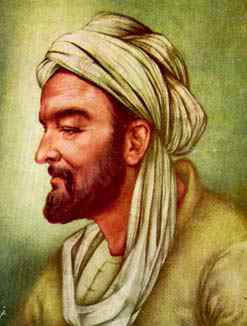
\includegraphics[width=1.5cm]{assets/sina.jpeg}}; 
	\begin{scope}[every node/.style={fill=white,rectangle,draw}]
		\path[->] (ibn) edge node[xshift=8mm,yshift=3mm] {was born on} (w2);
		\path[<->] (ibn) edge node[yshift=3mm] {was spouse of} (w4);
		\path[->] (ibn) edge node[xshift=-6mm,yshift=-3mm] {died on} (w3);
		\path[->] (ibn) edge node[xshift=9mm,yshift=-2mm] {was child of} (w5);
		\path[->] (ibn) edge node[yshift=-2mm] {was child of} (w6);
		\path[->] (ibn) edge node[xshift=-6mm] {died in} (w7);
		\path[->] (ibn) edge node[xshift=8mm,yshift=2mm] {was born in} (w8);
		\path[->] (ibn) edge node[xshift=-8mm,yshift=3mm] {has picture} (w9);
	\end{scope}
	\end{tikzpicture}
\end{center}

You might notice that I labeled the `edges' (arrows) in this graph (diagram). This is because we are dealing with multiple different relations between the `nodes'. These `nodes' all link together with relations and Google then presents these relational predicates to you in an understandable way. There is an entire field in Computer Science which deals with the relations between data and how to organize it into these sorts of structures, confusingly called `Ontology' (Philosophy also has a field named that, dealing with the question `what exists?'). These data structures and organizations, fundamentally, reduce to constructing interpretations for a particular domain (namely, the relevant data/information in the computer system).   

\chapter{Part 22 Truth in QL}
We have introduced you to interpretations. Since, among other things, they tell us which predicates are true of which objects, they will provide us with an account of the truth of atomic sentences. However, we now need to say, precisely, what it is for an arbitrary QL sentence to be true or false in an interpretation. We know from the previous content that there are three kinds of sentence in QL:
\begin{ebullet}
\item[\textbullet]atomic sentences
\item[\textbullet]sentences whose main logical operator is a sentential connective 
\item[\textbullet]sentences whose main logical operator is a quantifier
\end{ebullet}
We need to explain truth for all three kinds of sentence. We will provide a completely general explanation in this section. For some spoilers, atomic sentences are handled similarly to PL, connectives are almost identical to PL, and quantifiers are a bit finicky.  Throughout this section, we will be using the following interpretation/symbolization key for the examples. You should keep these in mind so that you can best understand why somethings work and others do not. 
\begin{ekey}
\item[domain] all people born before 2000ce
\item[a] Aristotle
\item[b] Beyoncé
\item[Px] x is a philosopher
\item[Rxy] x was born before y
\end{ekey}
\section{Part 22.1 Atomic Sentences}
The truth of atomic sentences should be fairly straightforward. For sentence letters, the interpretation specifies if it is true or false. The sentence ‘Pa’ should be true just in case ‘Px’ is true of ‘a’. Given our go-to interpretation, this is true iff Aristotle is a philosopher. Aristotle is a philosopher. So the sentence is true. Equally, ‘Pb’ is false on our go-to interpretation. Likewise, on this interpretation, ‘Rab’ is true iff the object named by ‘a’ was born before the object named by ‘b’. Well, Aristotle was born before Beyoncé. So ‘Rab’ is true. Equally, ‘Raa’ is false: Aristotle was not born before Aristotle.

Dealing with atomic sentences, then, is very intuitive. 
\factoidbox{
When R is a one-place predicate and a is a name, the sentence Ra is true in an interpretation IFF R is true of the object named by a.\\ 
When R is an n-place predicate and $a_1, a_2, \ldots , a_n$ are names, the sentence R$a_{1}a_{2}\ldots a_{n}$ is true in an interpretation iff R is true of the objects named by $a_1, a_2, \ldots , a_n$ (in that order) in that interpretation.}
\section{Part 22.2 Connectives}
Remember that QL sentences can be built up from simpler ones using the truth-functional connectives that were familiar from PL. The rules governing these truth-functional connectives are exactly the same as they were when we considered PL. Here they are:
\factoidbox{
\metav{A}\eand \metav{B} is true in an interpretation iff both \metav{A} is true and \metav{B} is true in that interpretation\\
\metav{A}\eor \metav{B} is true in an interpretation iff either \metav{A} is true or \metav{B} is true in that interpretation\\
\enot \metav{A} is true in an interpretation iff \metav{A} is false in that interpretation\\
\metav{A}\eif \metav{B} is true in an interpretation iff either \metav{A} is false or \metav{B} is true in that interpretation\\
\metav{A}\eiff \metav{B} is true in an interpretation iff A has the same truth value as B in that interpretation\\
}
This presents the very same information as the characteristic truth tables for the connectives; it just does so in a slightly different way. As an added note, you need to be extra careful to make sure that the connective is the main operator. This was easy enough in PL because we only had sentence letters and connectives. In QL, however, we also have quantifiers, which we will cover next. If a quantifier is the main operator, then you must work through it first before you can handle the connectives. Some examples will probably help to illustrate the idea. (Make sure you understand them!) On our go-to interpretation:
\factoidbox{
 ‘Rab\eand Pa’ is true\\
‘Rab\eand Pb’ is false because, although ‘Rab’ is true, ‘Pb’ is false\\
‘Pb\eor Pa’ is true\\
‘Pa\eand \enot (Rba\eand Rab)’ is true, because ‘Pa’ is true and ‘Rba' is false\\
}
Make sure you understand these examples.
\section{Part 22.3 Quantifiers}
The exciting innovation in QL, though, is the use of quantifiers, but expressing the truth conditions for quantified sentences is a bit more fiddly than one might first expect. We will go through three different ways in which one could understand the truth conditions for quantifiers (the third being the correct one). 

\subsection{The First Way to Think About Them}

Here is a naïve first thought. We want to say that ‘$\forall$x Fx’ is true iff ‘Fx’ is true of everything in the domain. This should not be too problematic: our interpretation will specify directly what ‘Fx’ is true of.

Unfortunately, this naïve thought is not general enough. For example, we want to be able to say that ‘$\forall$x$\exists$y Lxy’ is true just in case (speaking roughly) ‘$\exists$y Lxy’ is true of everything in the domain. But our interpretation does not directly specify what ‘$\exists$y Lxy’ is true of. Instead, whether or not this is true of something should follow just from the interpretation of the predicate ‘L’, the domain, and the meanings of the quantifiers.

\subsection{The Second Way}

So here is a second naïve thought. We might try to say that ‘$\forall$x$\exists$y Lxy’ is to be true in an interpretation iff $\exists$y Lay is true for every name a that we have included in our interpretation. Similarly, we might try to say that $\exists$y Lay is true just in case Lab is true for some name b that we have included in our interpretation.

Unfortunately, this is not right either. To see this, observe that our go-to interpretation only interprets two names, ‘a’ and ‘b’. But the domain—all people born before the year 2000ce— contains many more than two people. (And we have no intention of trying to correct for this by naming all of them!)

\subsection{The Correct Way}

Although it is not the case that we have named everyone, each person could have been given a name. So we should focus on this possibility of extending an interpretation by adding a new name. We will offer a few examples of how this might work, centering on our go-to interpretation, and we will then present the formal definition.

In our go-to interpretation, ‘$\exists$x Rbx’ should be true. After all, in the domain, there is certainly someone who was born after Beyoncé. Lady Gaga is one of those people. Indeed, if we were to extend our go-to interpretation—temporarily, mind—by adding the name ‘c’ to refer to Lady Gaga, then ‘Rbc’ would be true on this extended interpretation. This, surely, should suffice to make ‘$\exists$x Rbx’ true on the original go-to interpretation.

In our go-to interpretation, ‘$\exists$x (Px\eand Rxa)’ should also be true. After all, in the domain, there is certainly someone who was both a philosopher and born before Aristotle. Socrates is one such person. Indeed, if we were to extend our go-to interpretation by letting a new name, ‘c’, denote Socrates, then ‘Wc\eand Rca’ would be true on this extended interpretation. Again, this should surely suffice to make ‘$\exists$x (Px\eand Rxa)’ true on the original go-to interpretation.

In our go-to interpretation, ‘$\forall$x$\exists$y Rxy’ should be false. After all, consider the last person born in the year 1999. We don’t know who that was, but if we were to extend our go-to interpretation by letting a new name, ‘d’, denote that person, then we would not be able to find anyone else in the domain to denote with some further new name, perhaps ‘e’, in such a way that ‘Rde’ would be true. Indeed, no matter whom we named with ‘e’, ‘Rde’ would be false. This observation is surely sufficient to make ‘$\exists$y Rdy’ false in our extended interpretation, which in turn is surely sufficient to make ‘$\forall$x$\exists$y Rxy’ false on the original go-to interpretation.

If you have understood these three examples, that’s what matters. It provides the basis for a formal definition of truth for quantified sentences. Strictly speaking, though, we still need to give that definition. The result, sadly, is a bit ugly, and requires a few new definitions. Brace yourself!

Suppose that A is a formula containing at least one occurrence of the variable x, and that x is free in A. We will write this thus:
\begin{center}
A\ldots x\ldots x\ldots 
\end{center}
Suppose also that c is a name. Then we will write:
\begin{center}
A\ldots c\ldots c\ldots 
\end{center}
for the formula we obtain by replacing every occurrence of x in A with c. The resulting formula is called a substitution instance of $\forall$xA and $\exists$xA. Also, c is called the instantiating name. So:
\begin{center}
$\exists$x (Rex\eiff Fx)
\end{center}
is a substitution instance of
\begin{center}
$\forall$y$\exists$x (Ryx\eiff Fx)
\end{center}
with the instantiating name ‘e’ and instantiated variable ‘y’.

Our interpretation will include a specification of which names correspond to which objects in the domain. Take any object in the domain, say, d, and a name c which is not already assigned by the interpretation. If our interpretation is I, then we can consider the interpretation I[d/c] which is just like I except it also assigns the name c to the object d. Then we can say that d satisfies the formula A\ldots x\ldots x\ldots  in the interpretation I if and only if A\ldots c\ldots c\ldots  is true in I[d/c]. (If d satisfies A\ldots x\ldots x\ldots  we also say that A\ldots x\ldots x\ldots  is true of d.)

The interpretation I[d/c] is just like the interpretation I except it also assigns the name c to the object d.
An object d satisfies A\ldots x\ldots x\ldots  in interpretation I iff A\ldots c\ldots c\ldots  is true in I[d/c].

So, for instance, Socrates satisfies the formula Px since Pc is true in the interpretation I[Socrates/c], i.e., the interpretation:
\begin{ekey}
\item[domain] all people born before 2000ce
\item[a] Aristotle
\item[b] Beyoncé
\item[c] Socrates
\item[Px] x is a philosopher
\item[Rxy] x was born before y
\end{ekey}
Armed with this notation, the rough idea is as follows. The sentence $\forall$xA\ldots x\ldots x\ldots  will be true in I iff, for any object d in the domain, A\ldots c\ldots c\ldots  is true in I[d/c], i.e., no matter what object (in the domain) we name with c. In other words, $\forall$xA\ldots x\ldots x\ldots  is true iff every object in the domain satisfies A\ldots x\ldots x\ldots  Similarly, the sentence $\exists$xA will be true iff there is some object that satisfies A\ldots x\ldots x\ldots , i.e., A\ldots c\ldots c\ldots  true in I[d/c] for some object d.
\factoidbox{
$\forall$xA\ldots x\ldots x\ldots  is true in an interpretation iff every object in the domain satisfies A\ldots x\ldots x\ldots \\
$\exists$xA\ldots x\ldots x\ldots  is true in an interpretation iff at least one object in the domain satisfies A\ldots x\ldots x\ldots 
}
To be clear: all this is doing is formalizing (very pedantically) the intuitive idea expressed on the previous page. The result is a bit ugly, and the final definition might look a bit opaque. Hopefully, though, the spirit of the idea is clear.

\ockham

\practiceproblems
\problempart
\label{pr.TorF1}
Consider the following interpretation:
	\begin{ebullet}
		\item The domain comprises only Corwin and Benedict
		\item `$\atom{A}{x}$' is to be true of both Corwin and Benedict
		\item `$\atom{B}{x}$' is to be true of Benedict only
		\item `$\atom{N}{x}$' is to be true of no one
		\item `$c$' is to refer to Corwin
	\end{ebullet}
Determine whether each of the following sentences is true or false in that interpretation:
\begin{enumerate}
\item $\atom{B}{c} $
\item $\atom{A}{c}  \eiff \enot \atom{N}{c}$
\item $\atom{N}{c}  \eif (\atom{A}{c} \eor \atom{B}{c})$
\item $\forall x\, \atom{A}{x}$
\item $\forall x \enot \atom{B}{x}$
\item $\exists x(\atom{A}{x} \eand \atom{B}{x})$
\item $\exists x(\atom{A}{x} \eif \atom{N}{x})$
\item $\forall x(\atom{N}{x} \eor \enot \atom{N}{x})$
\item $\exists x\, \atom{B}{x} \eif \forall x\, \atom{A}{x}$
\end{enumerate}

\problempart
\label{pr.TorF2}
Consider the following interpretation:	
	\begin{ebullet}
		\item The domain comprises only Lemmy, Courtney and Eddy
		\item `$\atom{G}{x}$' is to be true of Lemmy, Courtney and Eddy.
		\item `$\atom{H}{x}$' is to be true of and only of Courtney
		\item `$\atom{M}{x}$' is to be true of and only of Lemmy and Eddy
		\item `$c$' is to refer to Courtney
		\item `$e$' is to refer to Eddy
	\end{ebullet}
Determine whether each of the following sentences is true or false in that interpretation:
\begin{enumerate}
\item $\atom{H}{c} $
\item $\atom{H}{e} $
\item $\atom{M}{c}  \eor \atom{M}{e}$
\item $\atom{G}{c}  \eor \enot \atom{G}{c}$
\item $\atom{M}{c}  \eif \atom{G}{c}$
\item $\exists x\, \atom{H}{x}$
\item $\forall x\, \atom{H}{x}$
\item $\exists x\, \enot \atom{M}{x}$
\item $\exists x(\atom{H}{x} \eand \atom{G}{x})$
\item $\exists x(\atom{M}{x} \eand \atom{G}{x})$
\item $\forall x(\atom{H}{x} \eor \atom{M}{x})$
\item $\exists x\, \atom{H}{x} \eand \exists x\, \atom{M}{x}$
\item $\forall x(\atom{H}{x} \eiff \enot \atom{M}{x})$
\item $\exists x\, \atom{G}{x} \eand \exists x \enot \atom{G}{x}$
\item $\forall x\exists y(\atom{G}{x} \eand \atom{H}{y})$
\end{enumerate}

\chapter{Part 23 Semantic Concepts and Validity}
\section{Part 23.1: Semantic Concepts}
Defining truth in QL was quite fiddly. But now that we are done, we can define various other central logical notions. These definitions will look very similar to those for PL, from Part 9. However, remember that they concern interpretations, rather than valuations. We will use the symbol ‘$\entails$’ for QL much as we did for PL. So:
\begin{center}
$A_1,A_2,\ldots,A_n$ $\entails$ C
\end{center}
means that there is no interpretation in which all of $A_1,A_2,\ldots,A_n$ are true and in which C is false. Derivatively,
\begin{center}
$\entails$ A
\end{center}
means that A is true in every interpretation, which is the same as saying that it can be proved from nothing. The other logical notions also have corresponding definitions in QL:
\factoidbox{\begin{ebullet}
\item[\textbullet] A QL sentence A is a tautology iff A is true in every interpretation; i.e., $\entails$ A. On the other hand, A is a contradiction iff A is false in every interpretation; i.e., $\entails$ \enot A.
\item[\textbullet] $A_1,A_2,\ldots,A_n$ \therefore C is valid in QL iff there is no interpretation in which all of the premises are true and the conclusion is false; i.e., $A_1,A_2,\ldots,A_n$ $\entails$ C. It is invalid in QL otherwise.
\item[\textbullet] Two QL sentences A and B are equivalent iff they are true in exactly the same interpretations as each other; i.e., both A $\entails$ B and B $\entails$ A.
\item[\textbullet] The QL sentences $A_1,A_2,\ldots,A_n$ are jointly satisfiable iff some interpretation makes all of them true. They are jointly unsatisfiable iff there is no such interpretation.
\end{ebullet}}
\section{Part 23.2 Using Interpretations}
\subsection{Tautologies and contradictions}

Suppose we want to show that ‘$\exists$x Axx\eif Bd’ is not a tautology. This requires showing that the sentence is not true in every interpretation; i.e., that it is false in some interpretation. If we can provide just one interpretation in which the sentence is false, then we will have shown that the sentence is not a tautology.

In order for ‘$\exists$x Axx\eif Bd’ to be false, the antecedent (‘$\exists$x Axx’) must be true, and the consequent (‘Bd’) must be false. To construct such an interpretation, we start by specifying a domain. Keeping the domain small makes it easier to specify what the predicates will be true of, so we will start with a domain that has just one member. For concreteness, let’s say it is just the city of Paris.

\begin{ekey}\item[domain]  Paris
\end{ekey}
From here, we will need to have some name, let's use ‘d’ and we have no option but:

\begin{ekey}\item[domain]  Paris
\item[d] Paris
\end{ekey}
Recall that we want ‘$\exists$x Axx’ to be true, so we want all members of the domain to be paired with themselves in the extension of ‘A’. We can just offer:

\begin{ekey}\item[domain]  Paris
\item[d] Paris
\item[Axy] x is identical with y
\end{ekey}
Now ‘Add’ is true, so it is surely true that ‘$\exists$x Axx’. Next, we want ‘Bd’ to be false, so the referent of ‘d’ must not be in the extension of ‘B’. We might simply offer:

\begin{ekey}\item[domain]  Paris
\item[d] Paris
\item[Axy] x is identical with y
\item[Bx] x is in Germany
\end{ekey}
Now we have an interpretation where ‘$\exists$x Axx’ is true, but where ‘Bd’ is false. So there is an interpretation where ‘$\exists$x Axx\eif Bd’ is false. So ‘$\exists$x Axx\eif Bd’ is not a tautology.

We can just as easily show that ‘$\exists$xAxx\eif Bd’ is not a contradiction. We need only specify an interpretation in which ‘$\exists$xA(x,x) \eif B(d)’ is true; i.e., an interpretation in which either ‘$\exists$x Axx’ is false or ‘Bd’ is true. Here is one:

\begin{ekey}\item[domain]  Paris
\item[d] Paris
\item[Axy] x is identical with y
\item[Bx] x is in France
\end{ekey}
This shows that there is an interpretation where ‘$\exists$xAxx\eif Bd’ is true. So ‘$\exists$x Axx\eif Bd’ is not a contradiction. For the conditions put exactly:
\factoidbox{
To show that A is not a tautology, it suffices to find an interpretation where A is false.\\
To show that A is not a contradiction, it suffices to find an interpretation where A is true.}
\subsection{Logical equivalence}

Suppose we want to show that ‘$\forall$x Sx’ and ‘$\exists$x Sx’ are not logically equivalent. We need to construct an interpretation in which the two sentences have different truth values; we want one of them to be true and the other to be false. We start by specifying a domain. Again, we make the domain small so that we can specify extensions easily. In this case, we will need at least two objects. (If we chose a domain with only one member, the two sentences would end up with the same truth value. In order to see why, try constructing some partial interpretations with one member domains.) For concreteness, let’s take:

\begin{ekey}\item[domain]  Ornette Coleman, Miles Davis
\end{ekey}
We can make ‘$\exists$x Sx’ true by including something in the extension of ‘S’, and we can make ‘$\forall$x Sx’ false by leaving something out of the extension of ‘S’. For concreteness, let’s say:

\begin{ekey}\item[domain]  Ornette Coleman, Miles Davis
\item[Sx] x plays saxophone
\end{ekey}
Now ‘$\exists$x Sx’ is true, because ‘Sx’ is true of Ornette Coleman. Slightly more precisely, extend our interpretation by allowing ‘c’ to name Ornette Coleman. ‘Sc’ is true in this extended interpretation, so ‘$\exists$x Sx’ was true in the original interpretation. Similarly, ‘$\forall$x Sx’ is false, because ‘Sx’ is false of Miles Davis. Slightly more precisely, extend our interpretation by allowing ‘d’ to name Miles Davis, and ‘Sd’ is false in this extended interpretation, so ‘$\forall$x Sx’ was false in the original interpretation. We have provided a counter-interpretation to the claim that ‘$\forall$x Sx’ and ‘$\exists$x Sx’ are logically equivalent. Here is the condition put concisely:

To show that A and B are not logically equivalent, it suffices to find an interpretation where one is true and the other is false. 
\subsection{Validity, entailment and satisfiability}

To test for validity, entailment, or satisfiability, we typically need to produce interpretations that determine the truth value of several sentences simultaneously. Consider the following argument in QL:
\begin{center}
$\exists$x (Gx\eif Ga) \therefore $\exists$x Gx\eif Ga
\end{center}
To show that this is invalid, we must make the premise true and the conclusion false. The conclusion is a conditional, so to make it false, the antecedent must be true and the consequent must be false. Clearly, our domain must contain two objects. Let’s try:

\begin{ekey}\item[domain]  Karl Marx, Ludwig von Mises
\item[Gx] x hated communism
\item[a] Karl Marx
\end{ekey}
Given that Marx wrote The Communist Manifesto, ‘Ga’ is plainly false in this interpretation. But von Mises famously hated communism, so ‘$\exists$x Gx’ is true in this interpretation. Hence ‘$\exists$x Gx \eif Ga’ is false, as required.

Does this interpretation make the premise true? Yes it does! Note that ‘Ga\eif Ga’ is true. (Indeed, it is a tautology.) But then certainly ‘$\exists$x (Gx\eif Ga)’ is true, so the premise is true, and the conclusion is false, in this interpretation. The argument is therefore invalid.

In passing, note that we have also shown that ‘$\exists$x (Gx\eif Ga)’ does not entail ‘$\exists$x Gx\eif Ga’, i.e., that $\exists$x (Gx\eif Ga) $\nvDash$ $\exists$xGx\eif Ga. Equally, we have shown that the sentences ‘$\exists$x (Gx\eif Ga)’ and ‘\enot ($\exists$xGx\eif Ga)’ are jointly satisfiable.

Let’s consider a second example. Consider:

$\forall$x$\exists$y Lxy \therefore $\exists$y$\forall$x Lxy

Again, we want to show that this is invalid. To do this, we must make the premises true and the conclusion false. Here is a suggestion:

\begin{ekey}\item[domain]  Canadian citizens currently in a domestic partnership with another Canadian citizen
\item[Lxy] x is in a domestic partnership with y
\end{ekey}
The premise is clearly true on this interpretation. Anyone in the domain is a Canadian citizen in a domestic partnership with some other Canadian citizen. That other citizen will also, then, be in the domain. So for everyone in the domain, there will be someone (else) in the domain with whom they are in a domestic partnership. Hence ‘$\forall$x$\exists$y Lxy’ is true. However, the conclusion is clearly false, for that would require that there is some single person who is in a domestic partnership with everyone in the domain, and there is no such person, so the argument is invalid. We observe immediately that the sentences ‘$\forall$x$\exists$y Lxy’ and ‘\enot $\exists$y$\forall$x Lxy’ are jointly satisfiable and that ‘$\forall$x$\exists$y Lxy’ does not entail ‘$\exists$y$\forall$x Lxy’.

For our third example, we’ll mix things up a bit. Previously, we described how we can present some interpretations using diagrams. For example:

\begin{center}
	\begin{tikzpicture}[modal]
		\node[world] (w1) {1};
		\node[world] (w2) [right=of w1]{2};
		\node[world] (w3) [below=of w2]{3};
		\path[->] (w1) edge[reflexive above] (w1);
		\path[->] (w1) edge (w2);
		\path[->] (w2) edge (w3);
		\path[->] (w1) edge (w3);
	\end{tikzpicture}
\end{center}

Using the conventions employed previously, the domain of this interpretation is the first three positive whole numbers, and ‘Rxy’ is true of x and y just in case there is an arrow from x to y in our diagram. Here are some sentences that the interpretation makes true:
\begin{earg}
\item[]$\forall$x$\exists$y Ryx
\item[]$\exists$x$\forall$y Rxy (loook at 1)
\item[]$\exists$x$\forall$y(Ryx\eiff Rxx)  (look at 1)
\item[]$\exists$x$\exists$y$\exists$z( (\enot Rxx\eand Rxy)\eand Rzx) (look at 2)
\item[]$\exists$x$\forall$y \enot Rxy (look at 3)
\item[]$\exists$x ($\exists$y Ryx\eand \enot $\exists$y Rxy) (look at 3)
\end{earg}
This immediately shows that all of the preceding six sentences are jointly satisfiable. We can use this observation to generate invalid arguments, e.g.:
\begin{earg}
\item[]$\forall$x$\exists$y Ryx,$\exists$x$\forall$y Rxy \therefore $\forall$x$\exists$y Rxy
\item[]$\exists$x$\forall$y Rxy,$\exists$x$\forall$y\enot Rxy \therefore \enot $\exists$x$\exists$y$\exists$z(\enot y=z\eand (Rxy\eand Rzx))
\item[]and many more besides.
\end{earg}
\factoidbox{
If some interpretation makes all of $A_1,A_2,\ldots,A_n$ true and C is false, then:
\begin{earg}
\item[]$A_1,A_2,\ldots,A_n$\therefore C is invalid
\item[]$A_1,A_2,\ldots,A_n$ $\nvDash$ C
\item[]$A_1,A_2,\ldots,A_n$,\enot C are jointly satisfiable.
\end{earg}
}

An interpretation which refutes a claim—to logical truth, say, or to entailment—is called a \gls{counter-interpretation}, or a \gls{countermodel}.


\newglossaryentry{counter-interpretation}
{
name={counter-interpretation},
text={counter-interpreation},
description={An interpretation which disproves the validity of an argument in QL}
}

\newglossaryentry{countermodel}
{
name={countermodel},
text={countermodel},
description={A diagram or model which is used to represent a counter-interpretation in QL or used to demonstrate the invalidity of an argument in ML}
}


We’ll close this section, though, with a caution about the relationship between (in)validity and (non)entailment. Recall QL’s limitations: it is is an extensional language; it ignores issues of vagueness; and it cannot handle cases of validity for ‘special reasons’. To take one illustration of these issues, consider this natural-language argument:
\begin{center}
Every fox is cute. \therefore All vixens are cute.
\end{center}
This is valid: necessarily every vixen is a fox, so it is impossible for the premise to be true and the conclusion false. Now, we might sensibly symbolize the argument as follows:
\begin{center}
$\forall$x (Fx\eif Cx) \therefore $\forall$x (Vx\eif Cx)
\end{center}
However, it is easy to find counter-models which show that $\forall$x (Fx\eif Cx) $\nvDash$ $\forall$x (Vx\eif Cx). (As a fun exercise, try to find one.) So, it would be wrong to infer that the English argument is invalid, just because there is a counter-model to the relevant QL-entailment.

The general moral is this. If you want to infer from the absence of an entailment in QL to the invalidity of some English argument, then you need to argue that nothing important is lost in the way you have symbolized the English argument.

\practiceproblems

\problempart
\label{pr.Contingent}
Show that each of the following is neither a validity nor a contradiction:
\begin{enumerate}
\item \leftsolutions\ $\atom{D}{a}  \eand \atom{D}{b}$
\item \leftsolutions\ $\exists x\, \atom{T}{xh}$
\item \leftsolutions\ $\atom{P}{m}  \eand \enot\forall x\, \atom{P}{x}$
\item $\forall z \atom{J}{z} \eiff \exists y\, \atom{J}{y}$
\item $\forall x (\atom{W}{xmn} \eor \exists y\atom{L}{xy})$
\item $\exists x (\atom{G}{x} \eif \forall y\, \atom{M}{y})$
\end{enumerate}

\solutions
\problempart
\label{pr.NotEquiv}
Show that the following pairs of sentences are not logically equivalent.
\begin{enumerate}
\item $\atom{J}{a} $,  $\atom{K}{a}$
\item $\exists x\, \atom{J}{x}$,  $\atom{J}{m}$
\item $\forall x\, \atom{R}{xx}$, $\exists x\, \atom{R}{xx}$
\item $\exists x\, \atom{P}{x} \eif \atom{Q}{c}$, $\exists x (\atom{P}{x} \eif \atom{Q}{c})$
\item $\forall x(\atom{P}{x} \eif \enot \atom{Q}{x})$, $\exists x(\atom{P}{x} \eand \enot \atom{Q}{x})$
\item $\exists x(\atom{P}{x} \eand \atom{Q}{x})$, $\exists x(\atom{P}{x} \eif \atom{Q}{x})$
\item $\forall x(\atom{P}{x}\eif \atom{Q}{x})$, $\forall x(\atom{P}{x} \eand \atom{Q}{x})$
\item $\forall x\exists y\, \atom{R}{xy}$, $\exists x\forall y\, \atom{R}{xy}$
\item $\forall x\exists y\, \atom{R}{xy}$, $\forall x\exists y\, \atom{R}{yx}$
\end{enumerate}

\problempart
Show that the following sentences are jointly satisfiable:
\begin{enumerate}
\item  $\atom{M}{a}, \enot \atom{N}{a}, \atom{P}{a}, \enot \atom{Q}{a}$
\item $\atom{L}{ee}, \atom{L}{eg}, \enot \atom{L}{ge}, \enot \atom{L}{gg}$
\item $\enot (\atom{M}{a} \eand \exists x\, \atom{A}{x}), \atom{M}{a} \eor \atom{F}{a}, \forall x(\atom{F}{x} \eif \atom{A}{x})$
\item $\atom{M}{a} \eor \atom{M}{b}, \atom{M}{a} \eif \forall x \enot \atom{M}{x}$
\item $\forall y\, \atom{G}{y}, \forall x (\atom{G}{x} \eif \atom{H}{x}), \exists y \enot \atom{I}{y}$
\item $\exists x(\atom{B}{x} \eor \atom{A}{x}), \forall x \enot \atom{C}{x}, \forall x\bigl[(\atom{A}{x} \eand \atom{B}{x}) \eif \atom{C}{x}\bigr]$
\item $\exists x\, \atom{X}{x}, \exists x\, \atom{Y}{x}, \forall x(\atom{X}{x} \eiff \enot \atom{Y}{x})$
\item $\forall x(\atom{P}{x} \eor \atom{Q}{x}), \exists x\enot(\atom{Q}{x} \eand \atom{P}{x})$
\item $\exists z(\atom{N}{z} \eand \atom{O}{zz}), \forall x\forall y(\atom{O}{xy} \eif \atom{O}{yx})$
\item $\enot \exists x \forall y\, \atom{R}{xy}, \forall x \exists y\, \atom{R}{xy}$
%\item $\enot \atom{R}{aa}$, $\forall x (x=a \eor \atom{R}{xa})$
%\item $\forall x\forall y\forall z[(x=y \eor y=z )\eor x=z]$, $\exists x\exists y\ \enot x= y$
%\item $\exists x\exists y((\atom{Z}{x} \eand \atom{Z}{y} )\eand x=y)$, $\enot \atom{Z}{d}$, $d=e$
\end{enumerate}

\problempart
Show that the following arguments are invalid:
\begin{enumerate}
\item $\forall x(\atom{A}{x} \eif \atom{B}{x}) \therefore \exists x\, \atom{B}{x}$
\item $\forall x(\atom{R}{x} \eif \atom{D}{x}), \forall x(\atom{R}{x} \eif \atom{F}{x}) \therefore \exists x(\atom{D}{x} \eand \atom{F}{x})$
\item $\exists x(\atom{P}{x}\eif \atom{Q}{x}) \therefore \exists x\, \atom{P}{x}$
\item $\atom{N}{a} \eand \atom{N}{b} \eand \atom{N}{c} \therefore \forall x\, \atom{N}{x}$
\item $\atom{R}{d,e}, \exists x\, \atom{R}{xd} \therefore \atom{R}{ed}$
\item $\exists x(\atom{E}{x} \eand \atom{F}{x}), \exists x\, \atom{F}{x} \eif \exists x\, \atom{G}{x} \therefore \exists x(\atom{E}{x} \eand \atom{G}{x})$
\item $\forall x\, \atom{O}{xc}, \forall x\, \atom{O}{cx} \therefore \forall x\, \atom{O}{xx}$
\item $\exists x(\atom{J}{x} \eand \atom{K}{x}), \exists x \enot \atom{K}{x}, \exists x \enot \atom{J}{x} \therefore \exists x(\enot \atom{J}{x} \eand \enot \atom{K}{x})$
\item $\atom{L}{a,b} \eif \forall x\, \atom{L}{xb}, \exists x\, \atom{L}{x,b} \therefore \atom{L}{b,b}$
%\item $\forall x(\atom{D}{x} \eif \exists y\, \atom{T}{yx}) \therefore \exists y \exists z\ \enot y= z$
\end{enumerate}



\section{Part 23.3: Reasoning about All Interpretations}
\label{allinterp}
\subsection{Tautologies and contradictions}

We can show that a sentence is not a tautology just by providing one carefully specified interpretation: an interpretation in which the sentence is false. To show that something is a tautology, on the other hand, it would not be enough to construct ten, one hundred, or even a thousand interpretations in which the sentence is true. A sentence is only a tautology if it is true in every interpretation, and there are infinitely many interpretations. We need to reason about all of them, and we cannot do this by dealing with them one by one!

Sometimes, we can reason about all interpretations fairly easily. For example, we can offer a relatively simple argument that ‘Raa\eor \enot Raa’ is a tautology:

\factoidbox{
Any relevant interpretation will give ‘Raa’ a truth value. If ‘Raa’ is true in an interpretation, then ‘Raa\eor \enot Raa’ is true in that interpretation. If ‘Raa’ is false in an interpretation, then \enot Raa is true, and so ‘Raa\eor \enot Raa’ is true in that interpretation. These are the only alternatives. So ‘Raa\eor \enot Raa’ is true in every interpretation. Therefore, it is a tautology.}

This argument is valid, of course, and its conclusion is true. However, it is not an argument in QL. Rather, it is an argument in English about QL: it is an argument in the metalanguage.

Note another feature of the argument. Since the sentence in question contained no quantifiers, we did not need to think about how to interpret ‘a’ and ‘R’; the point was just that, however we interpreted them, ‘Raa’ would have some truth value or other. (We could ultimately have given the same argument concerning PL sentences; using ‘R' rather than ‘Raa'.)

Let’s have another example. The sentence ‘$\forall$x (Rxx\eor \enot Rxx)’ should obviously be a tautology. However, saying precisely why is quite tricky. We cannot say that ‘Rxx\eor \enot Rxx’ is true in every interpretation, since ‘Rxx\eor \enot Rxx’ is not even a sentence of QL (remember that ‘x’ is a variable, not a name). Instead, we should say something like this:
\factoidbox{
Consider some arbitrary interpretation. $\forall$x (Rxx\eor \enot Rxx) is true in our interpretation iff Rxx\eor \enot Rxx is satisfied by every object of its domain. Consider some arbitrary member of the domain, which, for convenience, we will call Fred. Either Fred satisfies Rxx or it does not. If Fred satisfies ‘Rxx’, then Fred also satisfies ‘Rxx\eor \enot Rxx’. If Fred does not satisfy ‘Rxx’, it does satisfy ‘\enot Rxx’ and so also ‘Rxx\eor \enot Rxx’. So either way, Fred satisfies ‘Rxx\eor \enot Rxx’. Since there was nothing special about Fred—we might have chosen any object—we see that every object in the domain satisfies ‘Rxx\eor \enot Rxx’. So ‘$\forall$x (Rxx\eor \enot Rxx)’ is true in our interpretation. But we chose our interpretation arbitrarily, so ‘$\forall$x (Rxx\eor \enot Rxx)’ is true in every interpretation. It is therefore a tautology.}

This is quite longwinded, but, as things stand, there is no alternative. This should seem very similar to the argument made about ‘Raa', and it is. It is the same general method, the difference is that we needed to talk about some generic member of the domain and give them some completely arbitrary name. Since we did not rely on anything about a particular member of the domain, we can generalize it to all of them. So, in order to show that a sentence is a tautology, we must reason about all interpretations.

\subsection{Other Cases}

Similar points hold of other cases too. Thus, we must reason about all interpretations if we want to show:
\factoidbox{
\begin{ebullet}
	\item[\textbullet]that a sentence is a contradiction; for this requires that it is false in every interpretation.
	\item[\textbullet]that two sentences are logically equivalent; for this requires that they have the same truth value in every interpretation.
	\item[\textbullet]that some sentences are jointly unsatisfiable; for this requires that there is no interpretation in which all of those sentences are true together; i.e. that, in every interpretation, at least one of those sentences is false.
	\item[\textbullet]that an argument is valid; for this requires that the conclusion is true in every interpretation where the premises are true.
	\item[\textbullet]that some sentences entail another sentence.
\end{ebullet}}

The problem is that, with the tools available to you so far, reasoning about all interpretations is a serious challenge! For a final example, here is a perfectly obvious entailment:
\begin{center}
$\forall$x (Hx\eand Jx) $\vDash$  $\forall$x Hx
\end{center}
After all, if everything is both H and J , then everything is H . But we can only establish the entailment by considering what must be true in every interpretation in which the premise is true. To show this, we would have to reason as follows:
\factoidbox{
Consider an arbitrary interpretation in which ‘$\forall$x (Hx\eand Jx)’ is true. It follows that ‘Hx\eand Jx’ is satisfied by every object in this interpretation. ‘Hx’ will, then, also be satisfied by every object. So it must be that ‘$\forall$x Hx’ is true in the interpretation. We’ve assumed nothing about the interpretation except that it was one in which ‘$\forall$x (Hx\eand Jx)’ is true. So any interpretation in which ‘$\forall$x (Hx\eand Jx)’ is true is one in which ‘$\forall$x Hx’ is true.
}
Even for a simple entailment like this one, the reasoning is somewhat complicated. For more complicated entailments, the reasoning can be extremely torturous. 

The following table summarizes whether a single interpretation or counter-interpretation suffices, or whether we must reason about all interpretations.\\
\begin{tabular}{l|ll}
&Yes&No\\
\hline
Tautology?&All Interpretations&One Counter-interpretation\\
Contradiction?&All Interpretations&One Counter-interpretation\\
Equivalent?&All Interpretations&One Counter-interpretation\\
Satisfiable?&One Interpretation&All Interpretations\\
Valid?&All Interpretations&One Counter-interpretation\\
Entailment?&All Interpretations&One Counter-interpretation\\
\end{tabular}

You might want to compare this table with the table at the end of the similar content for PL, they are very similar. The key difference resides in the fact that PL concerns truth tables, whereas QL concerns interpretations. This difference is deeply important, since each truth-table only ever has finitely many lines, so that a complete truth table is a relatively tractable object. By contrast, there are infinitely many interpretations for any given sentence(s), so that reasoning about all interpretations can be a deeply tricky business. To avoid this for arguments, one can use a natural deduction system for QL to prove the validity and entailment. We will be going over this next. So, to show that an argument is valid in QL, you need to make a proof and to show that it is invalid, you need to make a counter-interpretation.  

\newglossaryentry{interpretation}{
  name = {interpretation},
  description = {A specification of a \gls{domain} together with the objects the \glspl{name} pick out and which objects the \glspl{predicate} are true of}
}

\newglossaryentry{substitution instance}{
  name = substitution instance,
  description = {The result of replacing every free occurrence of a \gls{variable} in a \gls{formula} with a \gls{name}}
}

\newglossaryentry{tautology (in QL)}
{
name=tautology (in QL),
description={A \gls{sentence of QL} that is true in every \gls{interpretation}}
}

\newglossaryentry{contradiction of QL}
{
  name=contradiction (of QL),
  text=contradiction,
description={A \gls{sentence of QL} that is false in every \gls{interpretation}}
}

\newglossaryentry{valid in QL}
{
  name=validity of arguments (in QL),
  text = valid,
description={A property held by arguments; an argument is valid if and only if no \gls{interpretation} makes all premises true and the conclusion false}
}

\newglossaryentry{equivalent in QL}
{
  name=equivalence (in QL),
  text = equivalent,
description={A property held by pairs of \glspl{sentence of QL} if and only if the sentences have the same truth value in every \gls{interpretation}}
}

\newglossaryentry{satisfiable in QL}
{
  name=satisfiability (in QL),
  text=jointly satisfiable,
description={A property held by \glspl{sentence of QL} if and only if some \gls{interpretation} makes all the sentences true}
}


\part{Natural Deduction in QL 1}
\label{ch.qlnd1}
\addtocontents{toc}{\protect\mbox{}\protect\hrulefill\par}
\stepcounter{chapcount}\setcounter{seccount}{1}
\chapter{Part \thechapcount: The Basic Rules for QL}
\section{Part \thechapcount.\theseccount: The Rules in PL are Allowed In QL}\stepcounter{seccount}
The language of QL makes use of all of the connectives of PL. So proofs in QL will use all of the basic and derived rules from Propositional Logic. This means that we can prove, for example, this argument:
\begin{earg}
\item[]Everyone is wearing yellow stockings.
\item[]If everyone is wearing yellow stockings, then everyone is cross gartered.
\item[]If everyone is wearing yellow stockings and everyone is cross gartered, then Olivia is displeased.
\item[\therefore] Olivia is displeased.
\end{earg}
We can, with relative ease, make the following symbolization key and, from that, the following symbolization:
\begin{ekey}
\item[domain] people in Olivia's court (including Olivia)
\item[Yx] x is wearing yellow stockings.
\item[Cx] x is cross gartered.
\item[Dx] x is displeased.
\item[m] Malvolio
\item[o] Olivia
\end{ekey}
With this, we can symbolize the argument like so:
\begin{center}
$\forall$ xYx, $\forall$ xYx\eif $\forall$ xCx,($\forall$ xYx\eand $\forall$ xCx)\eif Do \therefore Do
\end{center}
Notice that to prove this, we do not need to mess around with the quantifiers, though there will be many arguments both in this class and in the real-world, so to speak, where you will need to fiddle with quantifiers. The extra symbols may look scary, but they can be treated as blocks which you can shift around. For this argument, we don't need to break down blocks which we haven't handled in similar arguments in PL. So, we can prove it like so:
\begin{fitchproof}
\hypo[1]{a}{\forall xYx}
\hypo[3]{c}{(\forall xYx \eand \forall  xCx) \eif Do}
\hypo[2]{b}{\forall  xYx \eif \forall  xCx}
\have[4]{d}{\forall  xCx}\ce{b,a}
\have[5]{e}{\forall  xYx\eand \forall xCx}\ai{a,d}
\have[6]{f}{Do}\ce{c,e}
\end{fitchproof}	

A key thing to remember is that when you use the operations from PL in QL, you need to be sure that the main operator, the connective which governs the entire sentence, is not a quantifier. In this module, you will be learning the introduction and the elimination rules for the quantifiers and in the next one, you will be learning the special equivalency rule(s) for quantifiers. That said, you can also use the equivalency rules from PL in QL without much worry. I have mentioned this a few times and likely will need to say it a few more, QL is an extension of PL, not a replacement. For example, take the following argument:
\begin{earg}
\item[]Malvolio found the letter.
\item[]If Malvolio found the letter, then he is wearing yellow stockings and is cross gartered.
\item[]If someone is wearing yellow stockings and is cross gartered, then Olivia is displeased.
\item[\therefore ] Olivia is displeased.
\end{earg}
Adding Lx: x found the letter to our symbolization key, we can symbolize this argument as:
\begin{center}
Lm,Lm\eif (Ym\eand Cm),$\exists$ x(Yx\eand Cx)\eif Do \therefore Do
\end{center}
Thinking about it for just a moment, one can see that this argument is certainly valid, but we cannot prove it using merely the rules in PL. The first few moves to get to the conclusion involve things which should be easily understandable and in our ‘mental theater'. But, to get to the conclusion, we need to be able to move from Malvolio is wearing yellow stockings and is cross gartered (Ym\eand Cm) to someone is wearing yellow stockings and is cross gartered ($\exists$ x(Yx\eand Cx)). Such a move, in ordinary reasoning, might seem obvious and we often gloss over it, without paying it much mind. It should be clear by now, however, that the Devil is in the details and when we gloss over a logical inference, there is a high liklihood that something could have gone wrong and lead us astray.
\section{Part \thechapcount.\theseccount: Universal Quantifier Rules (Elimination and Introduction)}\stepcounter{seccount}
\subsection{Universal elimination}
From the claim that everything is F, you can infer that any particular thing is F. You name it; it’s F. There are many examples of us using this sort of reasoning in daily life. For example, suppose that you are in a restaurant and the cooks are being very, very slow in delivering the orders. Since they are being so slow, you can be sure that everyone in the restaurant is hungry ('Hx'). From this, you can go from the general to the particular and say that your friend Drew ('d') in the restaurant is hungry. We can symbolize this argument like so:
\begin{center}
$\forall$  xHx \therefore  Hd
\end{center}
Often, this sort of logical move is implied, not made explicit. But, as I have mentioned before, the devil is in the details. If we are going to make an error in our reasoning, it is going to likely be in these sort of implied moves and good, logical thinkers cannot allow for these sorts of mistakes. Every logical move is explicit. For an example of this move being implied in ordinary reason but needs to be explicit in QL, take this argument, in English:
\begin{earg}
\item[]All parrots can talk.
\item[]Polly is a parrot.
\item[\therefore ] Polly can talk.
\end{earg}
This should seem like a familiar logical structure, as I have used it before in the previous content. Logically, we treat statements of the form "all X's are Y's" as conditionals, "for all x, if x is X, the x is Y". So, the above argument would be symbolized like this:
\begin{center}
$\forall$  x(Px\eif Tx),Pp \therefore  Tp
\end{center}
 The implied move, in both of the arguments above, is to go from a statement about all things to a statement about one thing in particular. This is not  an equivalency rule, it cannot be done on only parts of statements or statements where the universal quantifier is not the main operator (we will explore this more below). With that caveat in mind, we can prove the first argument with relative ease:
\begin{fitchproof}
\hypo[1]{a}{\forall xHx}
\have[2]{b}{Hd}\Ae{a}
\end{fitchproof}
Notice the citation there, $\forall$ E, this is Universal Elimination. We obtained line 2 by dropping the universal quantifier and replacing every instance of ‘x’ with ‘d'. If we supposed that Berry ('b') was also in the restaurant, we could have equally concluded with:

\begin{fitchproof}
\hypo[1]{a}{\forall xHx}
\have[2]{b}{Hb}\Ae{a}
\end{fitchproof}

We obtained line 2 here by dropping the universal quantifier and replacing every instance of ‘x’ with ‘b’. We could have done the same with any other name we wanted. This motivates the universal elimination rule ($\forall$E):
\factoidbox{\begin{fitchproof}
\have[m]{a}{\forall xA\ldots x\ldots x\ldots}
\have[n]{b}{A\ldots c\ldots c\ldots}\Ae{a}
\end{fitchproof}}

The notation here was introduced previously. The point is that you can obtain any substitution instance of a universally quantified formula: replace every instance of the quantified variable with any name you like. We should emphasize that (as with every elimination rule) you can only apply the $\forall$ E rule when the universal quantifier is the main logical operator. So the following is banned:
\begin{fitchproof}
\hypo[1]{a}{\forall xSx\eif Cr}
\have[2]{b}{Sb\eif Cr}\by{naughty attempt to invoke $\forall$E}{a}
\end{fitchproof}

This is illegitimate, since `$\forall$x'  is not the main logical operator in line 1. To see why, suppose that the domain is restaurant workers, ‘Sx' symbolizes "x is out sick", ‘Cx' symbolizes ‘x is closed', ‘b' is ‘Berry', and ‘r' is the restaurant. So, the argument would sound something like this in English:
\begin{earg}
\item[]If all the restaurant workers are out sick, then the restaurant is closed.
\item[\therefore] If Berry is out sick, then the restaurant is closed.
\end{earg}
This reasoning doesn't quite flow, a restaurant can function without one of its workers (though it will be a pain for the rest I am sure). This means that we can't do reasoning like this and be absolutely sure it will work. (If you still need a reminder as to why this sort of inference should be banned, reread Part 19.)
\subsection{Universal introduction}

Suppose you had shown of each particular thing that it is F (and that there are no other things to consider). Then you would be justified in claiming that everything is F. This would motivate the following proof rule. If you had established each and every single substitution instance of ‘$\forall$x Fx', then you can infer ‘$\forall$x Fx’.

Unfortunately, that rule would be utterly unusable. To establish each and every single substitution instance would require proving ‘Fa’, ‘Fb’, \ldots , ‘F$j_2$’, \ldots , ‘F$r_{79002}$’, \ldots , and so on. Indeed, since there are infinitely many names in QL, this process would never come to an end. So we could never apply that rule. We need to be a bit more cunning in coming up with our rule for introducing universal quantification. A solution will be inspired by considering:
\begin{center}
$\forall$x Fx \therefore  $\forall$y Fy
\end{center}
This argument should obviously be valid. After all, alphabetical variation ought to be a matter of taste, and of no logical consequence. But how might our proof system reflect this? Suppose we begin a proof thus:
\begin{fitchproof}
\hypo[1]{d}{\forall xFx}
\have[2]{b}{Fa}\Ae{d}
\end{fitchproof}

We have proved ‘Fa’.  And, of course, nothing stops us from using the same justification to prove ‘Fb’, ‘Fc’, \ldots , ‘F$j_2$’, \ldots , ‘F$r_{79002}$, \ldots , and so on until we run out of space, time, or patience. But reflecting on this, we see that there is a way to prove Fc, for any name c. And if we can do it for any thing, we should surely be able to say that ‘F’ is true of everything. This therefore justifies us in inferring ‘$\forall$y Fy’, thus:
\begin{fitchproof}
\hypo[1]{d}{\forall xFx}
\have[2]{b}{Fa}\Ae{d}
\have[3]{c}{\forall yFy}\Ai{b}
\end{fitchproof}

The crucial thought here is that ‘a’ was just some arbitrary name. There was nothing special about it—we might have chosen any other name—and still the proof would be fine. And this crucial thought motivates the universal introduction rule ($\forall$I):
\factoidbox{\begin{fitchproof}
\have[m]{a}{A\ldots c\ldots c\ldots}
\have[n]{b}{\forall xA\ldots x\ldots x\ldots}\Ai{a}
\end{fitchproof}
\textbullet c must not occur in any undischarged assumption
and also x must not occur in A\ldots c\ldots c\ldots}

A crucial aspect of this rule, though, is bound up in the first constraint. This constraint ensures that we are always reasoning at a sufficiently general level. To see the constraint in action, consider this terrible argument:
\begin{earg}
\item[]Everyone loves Kylie Minogue; 
\item[\therefore] everyone loves themselves.
\end{earg}
We might symbolize this obviously invalid inference pattern as:
\begin{center}
$\forall$ x Lxk \therefore  $\forall$ x Lxx
\end{center}
Now, suppose we tried to offer a proof that vindicates this argument:
\begin{fitchproof}
\hypo[1]{a}{\forall xLxk}
\have[2]{b}{Lkk}
\have[3]{c}{\forall xLxx}\by{naughty attempt to invoke $\forall$I}{b}
\end{fitchproof}

This is not allowed, because ‘k’ occurred already in an undischarged assumption, namely, on line 1. The crucial point is that, if we have made any assumptions about the object we are working with, then we are not reasoning generally enough to to use a rule like $\forall$ I.

Although the name may not occur in any undischarged assumption, it may occur in a discharged assumption. That is, it may occur in a subproof that we have already closed. For example, this is just fine:
\begin{fitchproof}
\open
	\hypo[1]{a}{Gd}\by{AS}{}
	\have[2]{b}{Gd}\by{R}{a}
\close
\have[3]{c}{Gd\eif Gd}\ci{a-b}
\have[4]{d}{\forall z(Gz\eif Gz)}\Ai{c}
\end{fitchproof}
In this case, there was nothing special about ‘d', either used or implied. It was just a random name, so we could generalize. This tells us that ‘$\forall$z (Gz\eif Gz)’ is a theorem. And that is as it should be.

We should emphasize one last point. As per the conventions covered previously, the use of $\forall$ I requires that we are replacing every instance of the name c in A\ldots c\ldots c\ldots  with the variable x. If we only replace some names and not others, we end up ‘proving’ silly things. For example, consider the argument:
\begin{earg}
\item[]Everyone is as old as themselves; so everyone is as old as Judi Dench.
\end{earg}
We might symbolise this as follows:
\begin{center}
$\forall$ x Oxx \therefore  $\forall$ x Oxd
\end{center}
But now suppose we tried to vindicate this terrible argument with the following:
\begin{fitchproof}
\hypo[1]{a}{\forall xOxx}
\have[2]{b}{Odd}
\have[3]{c}{\forall xOxd}\by{naughty attempt to invoke $\forall$I}{b}
\end{fitchproof}

Fortunately, our rules do not allow for us to do this: the attempted proof is banned, since it doesn’t replace every occurrence of ‘d’ in line 2 with an ‘x’.
\section{Part \thechapcount.\theseccount: Existential Quantifier Rules (Introduction and Elimination)}\stepcounter{seccount}
\subsection{Existential Introduction}

From the claim that some particular thing is F, you can infer that something is F. This should seem obvious and, as a result, we ought to allow:
\begin{fitchproof}
\hypo[1]{a}{Raad}
\have[2]{b}{\exists xRaax}\Ei{a}
\end{fitchproof}

Here, we have replaced the name ‘d’ with a variable ‘x’, and then existentially quantified over it. The reasoning, in words, might look like this:

\factoidbox{We know that Raad. ‘d' is a thing, so we know that for some thing, x, Raax. (which is, symbolically, ‘$\exists$ xRaax'.)}

At the time time, we could have applied the same reasoning to ‘a' and gotten similar results, this means that we can allow:
\begin{fitchproof}
\hypo[1]{a}{Rxxd}
\have[2]{b}{\exists xRxxd}\Ei{a}
\end{fitchproof}

Here we have replaced both instances of the name ‘a’ with a variable, and then existentially generalized. But we do not need to replace both instances of a name with a variable: if Narcissus loves himself, then there is someone who loves Narcissus. So we also allow:
\begin{fitchproof}
\hypo[1]{a}{Rxxd}
\have[2]{b}{\exists xRxad}\Ei{a}
\end{fitchproof}

Here we have replaced just one instance of the name ‘a’ with a variable, and then existentially generalized. These observations motivate our introduction rule, although to explain it, we will need to introduce some new notation. Where A is a sentence containing the name c, we can emphasize this by writing ‘A\ldots c\ldots c\ldots ’. We will write ‘A\ldots x\ldots c\ldots ’ to indicate any formula obtained by replacing some or all of the instances of the name c with the variable x. Armed with this, our introduction rule is:
\factoidbox{\begin{fitchproof}
\have[m]{a}{A\ldots c\ldots c\ldots}
\have[n]{b}{\exists xA\ldots x\ldots c\ldots}\Ei{a}
\end{fitchproof}
\textbullet x must not occur in A\ldots c\ldots c\ldots} 

The constraint is included to guarantee that any application of the rule yields a sentence of QL. Thus the following is allowed:
\begin{fitchproof}
\hypo[1]{a}{Raad}
\have[2]{b}{\exists xRxad}\Ei{a}
\have[3]{c}{\exists y\exists xRxyd}\Ei{b}
\end{fitchproof}
But this is banned:
\begin{fitchproof}
\hypo[1]{a}{Raad}
\have[2]{b}{\exists xRxad}\Ei{a}
\have[3]{c}{\exists x\exists xRxxd}\Ei{b}
\end{fitchproof}

since the expression on line 3 contains clashing variables, and so is not a sentence of QL.

\subsection{Existential elimination}

Suppose we know that something is F. The problem is that simply knowing this does not tell us which thing is F. So it would seem that from ‘$\exists$x Fx’ we cannot immediately conclude ‘Fa’, ‘F$e_{23}$’, or any other substitution instance of the sentence. What can we do? Suppose we know that something is F, and that everything which is F is also G. In (almost) natural English, we might reason thus:
\factoidbox{
Since something is F, there is some particular thing which is an F. We do not know anything about it, other than that it’s an F, but for convenience, let’s call it ‘Becky’. So: Becky is F. Since everything which is F is G, it follows that Becky is G. But since Becky is G, it follows that something is G. And nothing depended on which object, exactly, Becky was. So, something is G.}

We might try to capture this reasoning pattern in a proof as follows:
\begin{fitchproof}
\hypo[1]{a}{\exists xFx}
\hypo[2]{b}{\forall x(Fx\eif Gx)}
\open
\hypo[3]{c}{Fb}\by{AS}{}
\have[4]{d}{Fb\eif Gb}\Ae{b}
\have[5]{e}{Gb}\ce{d,c}
\have[6]{f}{\exists xGx}\Ei{e}
\close
\have[7]{g}{\exists x Gx}\Ae{a,c-f}	
\end{fitchproof}
Breaking this down: we started by writing down our assumptions. At line 3, we made an additional assumption: ‘Fb’. This was just a substitution instance of ‘$\exists$ x Fx’. On this assumption, we established ‘$\exists$ x Gx’. Note that we had made no special assumptions about the object named by ‘b’; we had only assumed that it satisfies ‘Fx’. So nothing depends upon which object it is. And line 1 told us that something satisfies ‘Fx’, so our reasoning pattern was perfectly general. We can discharge the specific assumption ‘F (b)’, and simply infer ‘$\exists$ x Gx’ on its own. Putting this together, we obtain the existential elimination rule ($\exists$E):
\factoidbox{\begin{fitchproof}
\have[m]{a}{\exists xA\ldots x\ldots x\ldots }
\open
\hypo[n]{b}{	A\ldots c\ldots c\ldots }\by{AS}{}
\have[p]{P}{\exists xB}
\close
\have[r]{R}{\exists xB}\Ee{a, b-P}	
\end{fitchproof}}

There are some essential rules to keep in mind for applying this:
\factoidbox{
\textbullet c must not occur in any assumption undischarged before line n\\
\textbullet c must not occur in $\exists$ xA\ldots x\ldots x\ldots \\
\textbullet c must not occur in $\exists$ xB}

As with universal introduction, the constraints are extremely important. To see why, consider the following terrible argument:
\begin{earg}
\item[]Tim Button is a lecturer.
\item[]Someone is not a lecturer.
\item[]So Tim Button is both a lecturer and not a lecturer.
\end{earg}
We might symbolize this obviously invalid inference pattern as follows:
\begin{center}
Lb,$\exists$ x \enot Lx \therefore  Lb\eand \enot Lb
\end{center}
Now, suppose we tried to offer a proof that vindicates this argument:
\begin{fitchproof}
\hypo[1]{a}{Lb}
\hypo[2]{b}{\exists x\enot Lx}
\open
	\hypo[3]{c}{\enot Lb}\by{AS}{}
	\have[4]{d}{Lb\eand \enot Lb}\ai{a,c}
\close
\have[5]{e}{Lb\eand \enot Lb}\by{naughty use of $\exists$E}{a,c-d}	
\end{fitchproof}
The last line of the proof is not allowed. The name that we used in our substitution instance for ‘$\exists$ x \enot Lx’ on line 3, namely ‘b’, occurs in line 4. The this would be no better:
\begin{fitchproof}
\hypo[1]{a}{Lb}
\hypo[2]{b}{\exists x\enot Lx}
\open
\hypo[3]{c}{\enot Lb}\by{AS}{}
\have[4]{d}{Lb\eand \enot Lb}\ai{a,c}
\have[5]{f}{\exists x(Lx\eand \enot Lx)}\Ei{d}
\close
\have[6]{e}{Lb\eand \enot Lb}\by{naughty attempt to invoke $\exists$E}{a, c-f}	
\end{fitchproof}

The last line is still not allowed. For the name that we used in our substitution instance for ‘$\exists$ x \enot Lx’, namely ‘b’, occurs in an undischarged assumption, namely line 1. The moral of the story is this. If you want to squeeze information out of an existential quantifier, choose a new name for your substitution instance. That way, you can guarantee that you meet all the constraints on the rule for $\exists$ E.

It will pay off to keep how this rule works in mind, as this sort of assumption, where you give a name to something and operate using that name, is generalized and applied to possible circumstances (called ‘worlds') in Modal Logics, which we will cover in Module 10.

\godel

\practiceproblems
\problempart
Explain why these two `proofs' are \emph{incorrect}. Also, provide interpretations which would invalidate the fallacious argument forms the `proofs' enshrine:
\begin{multicols}{2}
	\begin{fitchproof}
		\hypo{Rxx}{\forall x\, \atom{R}{x,x}}
		\have{Raa}{\atom{R}{a,a}}\Ae{Rxx}
		\have{Ray}{\forall y\, \atom{R}{a,y}}\Ai{Raa}
		\have{Rxy}{\forall x\, \forall y\, \atom{R}{x,y}}\Ai{Ray}
	\end{fitchproof}
	\begin{fitchproof}
		\hypo{AE}{\forall x\, \exists y\, \atom{R}{x,y}}
		\have{E}{\exists y\, \atom{R}{a,y}}\Ae{AE}
		\open
			\hypo{ass}{\atom{R}{a,a}}
			\have{Ex}{\exists x\, \atom{R}{x,x}}\Ei{ass}
		\close
		\have{con}{\exists x\, \atom{R}{x,x}}\Ee{E, ass-Ex}
	\end{fitchproof}
\end{multicols}

\problempart 
\label{pr.justifyFOLproof}
The following three proofs are missing their citations (rule and line numbers). Add them, to turn them into bona fide proofs.
\begin{enumerate}
\item \begin{fitchproof}
\hypo{p1}{\forall x\exists y(\atom{R}{x,y} \eor \atom{R}{y,x})}
\hypo{p2}{\forall x\,\enot \atom{R}{m,x}}
\have{3}{\exists y(\atom{R}{m,y} \eor \atom{R}{y,m})}{}
	\open
		\hypo{a1}{\atom{R}{m,a} \eor \atom{R}{a,m}}
		\have{a2}{\enot \atom{R}{m,a}}{}
		\have{a3}{\atom{R}{a,m}}{}
		\have{a4}{\exists x\, \atom{R}{x,m}}{}
	\close
\have{n}{\exists x\, \atom{R}{x,m}} {}
\end{fitchproof}

\item \begin{fitchproof}
\hypo{1}{\forall x(\exists y\,\atom{L}{x,y} \eif \forall z\,\atom{L}{z,x})}
\hypo{2}{\atom{L}{a,b}}
\have{3}{\exists y\,\atom{L}{a,y} \eif \forall z\atom{L}{z,a}}{}
\have{4}{\exists y\, \atom{L}{a,y}} {}
\have{5}{\forall z\, \atom{L}{z,a}} {}
\have{6}{\atom{L}{c,a}}{}
\have{7}{\exists y\,\atom{L}{c,y} \eif \forall z\,\atom{L}{z,c}}{}
\have{8}{\exists y\, \atom{L}{c,y}}{}
\have{9}{\forall z\, \atom{L}{z,c}}{}
\have{10}{\atom{L}{c,c}}{}
\have{11}{\forall x\, \atom{L}{x,x}}{}
\end{fitchproof}

\item \begin{fitchproof}
\hypo{a}{\forall x(\atom{J}{x} \eif \atom{K}{x})}
\hypo{b}{\exists x\,\forall y\, \atom{L}{x,y}}
\hypo{c}{\forall x\, \atom{J}{x}}
\open
	\hypo{2}{\forall y\, \atom{L}{a,y}}
	\have{3}{\atom{L}{a,a}}{}
	\have{d}{\atom{J}{a}}{}
	\have{e}{\atom{J}{a} \eif \atom{K}{a}}{}
	\have{f}{\atom{K}{a}}{}
	\have{4}{\atom{K}{a} \eand \atom{L}{a,a}}{}
	\have{5}{\exists x(\atom{K}{x} \eand \atom{L}{x,x})}{}
\close
\have{j}{\exists x(\atom{K}{x} \eand \atom{L}{x,x})}{}
\end{fitchproof}
\end{enumerate}

\problempart
\label{pr.BarbaraEtc.proof2}
Aristotle and his successors identified other syllogistic forms which depended upon `existential import'. Symbolize each of these argument forms in FOL and offer proofs.
\begin{enumerate}
	\item \textbf{Barbari.} Something is H. All G are F. All H are G. So: Some H is F
	\item \textbf{Celaront.} Something is H. No G are F. All H are G. So: Some H is not F
	\item \textbf{Cesaro.} Something is H. No F are G. All H are G. So: Some H is not F.
	\item \textbf{Camestros.} Something is H. All F are G. No H are G. So: Some H is not F.
	\item \textbf{Felapton.} Something is G. No G are F. All G are H. So: Some H is not F.
	\item \textbf{Darapti.} Something is G. All G are F. All G are H. So: Some H is F.
	\item \textbf{Calemos.} Something is H. All F are G. No G are H. So: Some H is not F.
	\item \textbf{Fesapo.} Something is G. No F is G. All G are H. So: Some H is not F.
	\item \textbf{Bamalip.} Something is F. All F are G. All G are H. So: Some H are F.
\end{enumerate}

\problempart
\label{pr.someFOLproofs}
Provide a proof of each claim.
\begin{enumerate}
\item $\proves \forall x\,\atom{F}{x} \eif \forall y(\atom{F}{y} \eand \atom{F}{y})$
\item $\forall x(\atom{A}{x}\eif \atom{B}{x}), \exists x\,\atom{A}{x} \proves \exists x\,\atom{B}{x}$
\item $\forall x(\atom{M}{x} \eiff \atom{N}{x}), \atom{M}{a} \eand \exists x\,\atom{R}{xa} \proves \exists x\,\atom{N}{x}$
\item $\forall x\, \forall y\,\atom{G}{xy}\proves\exists x\,\atom{G}{xx}$
\item $\proves\forall x\,\atom{R}{xx} \eif \exists x\, \exists y\,\atom{R}{xy}$
\item $\proves\forall y\, \exists x (\atom{Q}{y} \eif \atom{Q}{x})$
\item $\atom{N}{a} \eif \forall x(\atom{M}{x} \eiff \atom{M}{a}), \atom{M}{a}, \enot\atom{M}{b}\proves \enot \atom{N}{a}$
\item $\forall x\, \forall y (\atom{G}{xy} \eif \atom{G}{yx}) \proves \forall x\forall y (\atom{G}{xy} \eiff \atom{G}{yx})$
\item $\forall x(\enot\atom{M}{x} \eor \atom{L}{jx}), \forall x(\atom{B}{x}\eif \atom{L}{jx}), \forall x(\atom{M}{x}\eor \atom{B}{x})\proves \forall x\atom{L}{jx}$
\end{enumerate}

\problempart
\label{pr.likes}
Write a symbolization key for the following argument, symbolize it, and prove it:
\begin{quote}
There is someone who likes everyone who likes everyone that she likes. Therefore, there is someone who likes herself.
\end{quote}


\problempart
Show that each pair of sentences is provably equivalent.
\begin{enumerate}
\item $\forall x (\atom{A}{x}\eif \enot \atom{B}{x})$, $\enot\exists x(\atom{A}{x} \eand \atom{B}{x})$
\item $\forall x (\enot\atom{A}{x}\eif \atom{B}{d})$, $\forall x\,\atom{A}{x} \eor \atom{B}{d}$
\item $\exists x\,\atom{P}{x} \eif \atom{Q}{c}$, $\forall x (\atom{P}{x} \eif \atom{Q}{c})$
\end{enumerate}

\problempart
\label{pr.FOLequivornot}
For each of the following pairs of sentences: If they are provably equivalent, give proofs to show this. If they are not, construct an interpretation to show that they are not logically equivalent.
\begin{enumerate}
\item $\forall x\,\atom{P}{x} \eif \atom{Q}{c}, \forall x (\atom{P}{x} \eif \atom{Q}{c})$
\item $\forall x\,\forall y\, \forall z\,\atom{B}{xyz}, \forall x\,\atom{B}{xx}x$
\item $\forall x\,\forall y\,\atom{D}{xy}, \forall y\,\forall x\,\atom{D}{xy}$
\item $\exists x\,\forall y\,\atom{D}{xy}, \forall y\,\exists x\,\atom{D}{xy}$
\item $\forall x (\atom{R}{c,a} \eiff \atom{R}{xa}), \atom{R}{ca} \eiff \forall x\,\atom{R}{xa}$
\end{enumerate}

\problempart
\label{pr.FOLvalidornot}
For each of the following arguments: If it is valid in FOL, give a proof. If it is invalid, construct an interpretation to show that it is invalid.
\begin{enumerate}
\item $\exists y\,\forall x\,\atom{R}{xy} \therefore \forall x\,\exists y\,\atom{R}{xy}$
\item $\forall x\,\exists y\,\atom{R}{xy} \therefore  \exists y\,\forall x\,\atom{R}{xy}$
\item $\exists x(\atom{P}{x} \eand \enot \atom{Q}{x}) \therefore \forall x(\atom{P}{x} \eif \enot \atom{Q}{x})$
\item $\forall x(\atom{S}{x} \eif \atom{T}{a}), \atom{S}{d} \therefore \atom{T}{a}$
\item $\forall x(\atom{A}{x}\eif \atom{B}{x}), \forall x(\atom{B}{x} \eif \atom{C}{x}) \therefore \forall x(\atom{A}{x} \eif \atom{C}{x})$
\item $\exists x(\atom{D}{x} \eor \atom{E}{x}), \forall x(\atom{D}{x} \eif \atom{F}{x}) \therefore \exists x(\atom{D}{x} \eand \atom{F}{x})$
\item $\forall x\,\forall y(\atom{R}{xy} \eor \atom{R}{yx}) \therefore \atom{R}{jj}$
\item $\exists x\,\exists y(\atom{R}{xy} \eor \atom{R}{yx}) \therefore \atom{R}{jj}$
\item $\forall x\,\atom{P}{x} \eif \forall x\,\atom{Q}{x}, \exists x\, \enot\atom{P}{x} \therefore \exists x\, \enot \atom{Q}{x}$
\item $\exists x\,\atom{M}{x} \eif \exists x\,\atom{N}{x}$, $\enot \exists x\,\atom{N}{x}\therefore  \forall x\, \enot \atom{M}{x}$
\end{enumerate}



\stepcounter{chapcount}\setcounter{seccount}{1}
\chapter{Part \thechapcount: Tips for and an Example of Proofs in QL}

In \nameref{tips.pl}, we discussed strategies for constructing proofs using the basic rules of natural deduction for PL. The same principles apply to the rules for the quantifiers. If we want to prove a quantifier sentence $\forall$ xAx or $\exists$ xAx. We can work backward by justifying the sentence we want by $\forall$ I or $\exists$ I and trying to find a proof of the corresponding premise of that rule. And to work forward from a quantified sentence, we apply $\forall$ E or $\exists$ E, as the case may be.

Specifically, suppose you want to prove $\forall$ xAx. To do so using $\forall$ I, we would need a proof of Ac for some name c which does not occur in any undischarged assumption. To apply the corresponding strategy, i.e., to construct a proof of $\forall$ xAx by working backward, is thus to write Ac above it and then to continue to try to find a proof of that sentence.
\begin{fitchproof}
\ellipsesline					
\have[m]{b}{Ac}{}			
\have[n]{c}{\forall xAx}\Ai{b}	
\end{fitchproof}
Ac is obtained from Ax by replacing every free occurrence of x in Ax by c. For this to work, c must satisfy the special condition. We can ensure that it does by always picking a name that does not already occur in the proof constructed so far. (Of course, it will occur in the proof we end up constructing—just not in an assumption that is undischarged at line m.)

To work backward from a sentence $\exists$ xAx we similarly write a sentence above it that can serve as a justification for an application of the $\exists$ I rule, i.e., a sentence of the form Ac
\begin{fitchproof}
\ellipsesline
\have[m]{b}{Ac}{}
\have[n]{c}{\exists xAx}\Ei{b}	
\end{fitchproof}

This looks just like what we would do if we were working backward from a universally quantified sentence. The difference is that whereas for $\forall$ I we have to pick a name c which does not occur in the proof (so far), for $\exists$ I we may and in general must pick a name c which already occurs in the proof. Just like in the case of \eor I, it is often not clear which c will work out, and so to avoid having to backtrack you should work backward from existentially quantified sentences only when all other strategies have been applied.

By contrast, working forward from sentences $\exists$ xAx generally always works and you won’t have to backtrack. Working forward from an existentially quantified sentence takes into account not just $\exists$ xAx but also whatever sentence B you would like to prove. It requires that you set up a subproof above B, wherein B is the last line, and a substitution instance Ac of $\exists$ xAx as the assumption. In order to ensure that the condition on c that governs $\exists$ E is satisfied, chose a name c which does not already occur in the proof.
\begin{fitchproof}
\ellipsesline
\have[m]{b}{\exists xAx}				
\ellipsesline
\hypo[k]{k}{P_k}		
\open
\hypo[n]{d}{Ac}\by{AS}{}
\have[\ ]{e}{\ldots}	
\have[p]{f}{Bc}
\have[q]{g}{\exists xBx}\Ei{f}
\close
\have[r]{h}{\exists xBx}\Ee{b,d-g}	
\end{fitchproof}
You’ll then continue with the goal of proving B, but now inside a subproof in which you have an additional sentence to work with, namely Ac.

Lastly, working forward from $\forall$ xAx means that you can always write down Ac and justify it using $\forall$ E, for any name c. Of course, you wouldn’t want to do that willy-nilly. Only certain names c will help in your task of proving whatever goal sentence you are working on. So, like working backward from $\exists$ xAx, you should work forward from $\forall$ xAx only after all other strategies have been applied. Let’s consider as an example the argument:
\begin{center}
$\forall$ x(Ax\eif B) \therefore $\exists$ xAx\eif B
\end{center}
To start constructing a proof, we write the premise at the top and the conclusion at the bottom.
\begin{fitchproof}
\hypo{1}{\forall x(Ax \eif B)}
\ellipsesline
\have[r]{7}{\exists x\,Ax\eif B}
\end{fitchproof}
The strategies for connectives of PL still apply, and you should apply them in the same order: first work backward from conditionals, negated sentences, conjunctions, and now also universal quantifiers, then forward from disjunctions and now existential quantifiers, and only then try to apply \eif E, ¬E, \eor I, $\forall$ E, or $\exists$ I. In our case, that means, working backward from the conclusion:
\begin{fitchproof}
\hypo{1}{\forall x(Ax \eif B)}
\open
\hypo{2}{\exists xAx}\by{AS}{}
\ellipsesline
\have[q]{z}{B}
\close
\have[r]{7}{\exists x\,Ax\eif B}\ci{2-z}
\end{fitchproof}

Our next step should be to work forward from $\exists$ x Ax on line 2. For that, we have to pick a name not already in our proof. Since no names appear, we can pick any name, say ‘d’
\begin{fitchproof}
\hypo{1}{\forall x(Ax \eif B)}
\open
\hypo{2}{\exists xAx}\by{AS}{}
\open
\hypo{3}{Ad}\by{AS}{}
\ellipsesline
\have[p]{z}{B}
\close
\have[q]{y}{B}\Ee{2-z}
\close
\have[r]{7}{\exists x\,Ax\eif B}\ci{2-y}
\end{fitchproof}

Now we’ve exhausted our primary strategies, and it is time to work forward from the premise $\forall$ x (Ax \eif  B). Applying $\forall$ E means we can justify any instance of Ac \eif  B, regardless of what c we choose. Of course, we’ll do well to choose d, since that will give us Ad\eif B. Then we can apply \eif E to justify B, finishing the proof.
\begin{fitchproof}
\hypo{1}{\forall x(Ax \eif B}
\open
\hypo{2}{\exists xAx}\by{AS}{}
\open
\hypo{3}{Ad}\by{AS}{}
\have{4}{Ad\eif B}\Ae{1}
\have{5}{B}\ce{4,3}
\close
\have{6}{B}\Ee{2-5}
\close
\have{7}{\exists x\,Ax\eif B}\ci{2-6}
\end{fitchproof}

Now let’s construct a proof of the converse. We begin with

\begin{fitchproof}
\hypo{1}{\exists xAx \eif B}
\ellipsesline
\have[r]{7}{\forall x(Ax\eif B)}
\end{fitchproof}

Note that the premise is a conditional, not an existentially quantified sentence, so we should not (yet) work forward from it. Working backward from the conclusion, $\forall$ x (Ax \eif  B), leads us to look for a proof of Ad \eif  B:
\begin{fitchproof}
\hypo{1}{\exists xAx \eif B}
\ellipsesline
\have[q]{6}{Ad\eif B}
\have[r]{7}{\forall x(Ax\eif B)}\Ai{6}
\end{fitchproof}

And working backward from Ad\eif  B means we should set up a subproof with Ad as an assumption and B as the last line:
\begin{fitchproof}
\hypo{1}{\exists xAx \eif B}
\open
\hypo{2}{Ad}\by{AS}{}
\ellipsesline
\have[p]{5}{B}
\close
\have[q]{6}{Ad\eif B}\ci{2-5}
\have[r]{7}{\forall x(Ax\eif B)}\Ai{6}
\end{fitchproof}

Now we can work forward from the premise on line 1. That’s a conditional, and its consequent happens to be the sentence B we are trying to justify. So we should look for a proof of its antecedent, $\exists$ x Ax. Of course, that is now readily available, by $\exists$I from line 2, and we’re done:
\begin{fitchproof}
\hypo{1}{\exists xAx \eif B}
\open
\hypo{2}{Ad}\by{AS}{}
\have{3}{\exists xAx}\Ei{2}
\have{4}{B}\ce{1,3}
\close
\have{5}{Ad\eif B}\ci{2-4}
\have{6}{\forall x(Ax\eif B)}\Ai{5}
\end{fitchproof}

\part{Natural Deduction in QL 2}
\label{ch.qlnd2}
\addtocontents{toc}{\protect\mbox{}\protect\hrulefill\par}
\chapter{Part 26 Identity (‘=')}
\section{Part 26.1 Symbolizing Identity Statements}
\subsection{The Need for a New Connective/Predicate}

Thus far, you have everything necessary to work with QL and hopefully, apply it in your daily life, if we didn't have multiple ways of saying the same thing and we didn't obscure or leave out certain natural inferences. For example, consider this sentence:
\begin{earg}
\item[\ex{Pavel1}] Pavel owes money to everyone
\end{earg}
Let the domain be people; this will allow us to symbolize ‘everyone’ with a universal quantifier. Offering the symbolization key:
\begin{ekey}
\item[Oxy] x owes money to y
\item[p] Pavel
\end{ekey}
From this, we can symbolize sentence \ref{Pavel1} with ‘$\forall$xOpx’. But this has a (perhaps) odd consequence. It requires that Pavel owes money to every member of the domain (whatever the domain may be). The domain certainly includes Pavel. So this entails that Pavel owes money to himself. And maybe we did not want to say that. Maybe we meant to leave it open if Pavel owes money to himself, something we could have expressed more precisely by using either on of the following:
\begin{earg}
\item[\ex{Pavel2}] Pavel owes money to everyone \emph{else}
\item[\ex{Pavel3}] Pavel owes money to everyone \emph{other than Pavel}
\end{earg}
But we do not have any way for dealing with the italicised words yet. The solution is to add another symbol to QL.
\subsection{
Adding identity
}
The symbol ‘=’ will act as a two-place predicate; but, since it will have a special meaning, we shall write it a bit differently: we put it between two terms, rather than out front. (This should also be familiar; consider a mathematical equation like 1/2 = 0.5.) And the special meaning for ‘=’ is given by the fact that we always adopt the following symbolization key:
\begin{ekey}
\item[x=y] x is identical to y
\end{ekey}
This does not mean merely that the objects in question are indistinguishable, or that all of the same things are true of them. Rather, it means that the objects in question are the very same object. Also, we are using this symbol as a connective because of this very special meaning. Rather than connecting sentences, the identity symbol connects terms, names, and there are some special inference rules one can use involving this connective. To put this to use, suppose we want to symbolize this sentence:
\begin{earg}
\item[\ex{Pavel4}] Pavel is Mister Checkov.
\end{earg}
Let us add to our symbolization key:
\begin{ekey}
\item[c] Mister Checkov
\end{ekey}
Now sentence \ref{Pavel4} can be symbolized as ‘p=c’. This tells us that the names ‘p’ and ‘c’ both name the same thing. We can also now deal with sentences \ref{Pavel2} and \ref{Pavel3}. Both of these sentences can be paraphrased as ‘Everyone who is not Pavel is owed money by Pavel’. Paraphrasing some more, we get: ‘For all x, if x is not Pavel, then x is owed money by Pavel’. Now that we are armed with our new identity symbol, we can symbolize this as
\begin{center}
$\forall$x(\enot (x=p)\eif Opx)
\end{center}
You may notice that there are parentheses around ‘\enot (x=p)’, I have included those for clairity, as the identity symbol acts both as a predicate and as a connective. It is perfectly acceptable to write ‘\enot x=p’, though ahat might look a bit strange, because the symbol that comes immediately after the ‘\enot’ is a variable, rather than a predicate, but this is not a problem. We are simply negating the entire formula, ‘x=p’.
\subsection{
‘Only’ and ‘except’
}
In addition to sentences that use the word ‘else’, and ‘other than’, identity is helpful when symbolizing some sentences that contain the words ‘only’, and ‘except’. Consider:
\begin{earg}
\item[\ex{Pavel5}] Only Pavel owes money to Hikaru.
\end{earg}
Let ‘h’ name Hikaru. Plausibly, sentence \ref{Pavel5} is true if, and only if, both of the following conditions hold:
\begin{earg}
\item[\ex{Pavel6}] Pavel owes money to Hikaru.
\item[\ex{Pavel7}] No-one who is not Pavel owes money to Hikaru.
\end{earg}
Sentence \ref{Pavel7} can be symbolized by any one of:
\begin{earg}
\item[]\enot $\exists$x (\enot (x=p)\eand Oxh)
\item[]$\forall$x (\enot (x=p)\eif \enot Oxh)
\item[]$\forall$x (Oxh\eif (x=p))
\end{earg}
Thus, we can symbolize sentence \ref{Pavel5} as the conjunction of one of the above with the symbolization of \ref{Pavel6}, ‘Oph, or more compactly using ‘\eiff ’ as ‘$\forall$x(Oxh\eiff (x=p))’.
\begin{earg}
\item[\ex{Pavel8}] Everyone except Pavel owes money to Hikaru.
\end{earg}
Sentence \ref{Pavel8} can be treated similarly, although now of course Pavel does not owe Hikaru money. We can paraphrase it as ‘Everyone who is not Pavel owes Hikaru money, and Pavel does not’. Consequently, it can be symbolized as, ‘$\forall$x (\enot (x=p)\eif  Oxh)\eand \enot Oph’, or more concisely, ‘$\forall$x(\enot (x=p)\eiff Oxh)’. Other locutions akin to ‘except’ such as ‘but’ or ‘besides’ (as used in ‘no-one but Pavel’ or ‘someone besides Hikaru’) can be treated in similar ways.

The above treatment of so-called “exceptives” is not uncontentious. Some linguists think that sentence \ref{Pavel8} does not entail that Pavel doesn’t owe Hikaru money, and so the symbolization should just be ‘$\forall$x (\enot (x=p)\eif Oxh)’. There are also uses of ‘except’ that clearly do not have that entailment, especially in mathematical writing. For instance, you may read in a calculus textbook that “the function f is defined everywhere except possibly at a”. That means only that for every point x other than a, f is defined at x. It is not required that f is undefined at a; it’s left open whether f is or is not defined at a.

\subsection{There are at least\ldots}

We can also use identity to say how many things there are of a particular kind. For example, consider these sentences:
\begin{earg}
\item[\ex{apple1}] There is at least one apple
\item[\ex{apple2}] There are at least two apples
\item[\ex{apple3}] There are at least three apples
\end{earg}
We will use the symbolization key:
\begin{ekey}
\item[Ax] x is an apple
\end{ekey}
Sentence \ref{apple1} does not require identity. It can be adequately symbolized by ‘$\exists$x Ax’: There is an apple; perhaps many, but at least one.

It might be tempting to also symbolize sentence \ref{apple2} without identity. Yet consider the sentence ‘$\exists$x$\exists$y(Ax\eand Ay)’. Roughly, this says that there is some apple x in the domain and some apple y in the domain. Since nothing precludes these from being one and the same apple, this would be true even if there were only one apple. In order to make sure that we are dealing with different apples, we need an identity predicate. Sentence \ref{apple2} needs to say that the two apples that exist are not identical, so it can be symbolized by ‘$\exists$x$\exists$y( (Ax\eand Ay)\eand \enot (x=y))’.

Sentence \ref{apple3} requires talking about three different apples. Now we need three existential quantifiers, and we need to make sure that each will pick out something different:
\begin{center}
$\exists$x$\exists$y$\exists$z[((Ax\eand Ay)\eand Az)\eand ((\enot (x=y)\eand \enot (y=z))\eand \enot (x=z))]
\end{center}
Note that it is not enough to use ‘\enot (x=y)\eand \enot (y=z)’ to symbolize ‘x, y, and z are all different.’ For that would be true if x and y were different, but x=z. In general, to say that x1,\ldots, xn are all different, we must have a conjunction of \enot (xi=xj) for every different pair i and j .
\subsection{
There are at most\ldots
}
Now consider these sentences:
\begin{earg}
\item[\ex{appleonly1}] There is at most one apple
\item[\ex{appleonly2}] There are at most two apples
\end{earg}
Sentence \ref{appleonly1} can be paraphrased as, ‘It is not the case that there are at least two apples’. This is just the negation of sentence \ref{apple2}:
\begin{center}
\enot $\exists$x$\exists$y[(Ax \eand Ay)\eand \enot (x=y)]
\end{center}
But sentence \ref{appleonly1} can also be approached in another way. It means that if you pick out an object and it’s an apple, and then you pick out an object and it’s also an apple, you must have picked out the same object both times. With this in mind, it can be symbolized by
\begin{center}
$\forall$x$\forall$y[Ax\eand Ay)\eif (x=y)]
\end{center}
The two sentences will turn out to be logically equivalent.

Similarly, sentence \ref{appleonly2} can be approached in two equivalent ways. It can be paraphrased as, ‘It is not the case that there are three or more distinct apples’, so we can offer:
\begin{center}
\enot $\exists$x$\exists$y$\exists$z[((Ax\eand Ay)\eand Az)\eand ((\enot (x=y)\eand \enot (x=z))\eand \enot (y=z))]
\end{center}
Alternatively we can read it as saying that if you pick out an apple, and an apple, and an apple, then you will have picked out (at least) one of these objects more than once. Thus:
\begin{center}
$\forall$x$\forall$y$\forall$z((Ax\eand Ay)\eand Az)\eif (((x=y)\eor (x=z))\eor (y=z))]
\end{center}
\subsection{There are exactly\ldots}

We can now consider precise of numerical quantity, like:
\begin{earg}
\item[\ex{appleexact1}]There is exactly one apple.
\item[\ex{appleexact2}]There are exactly two apples.
\item[\ex{appleexact3}]There are exactly three apples.
\end{earg}
Sentence \ref{appleexact1} can be paraphrased as, ‘There is at least one apple and there is at most one apple’. This is just the conjunction of sentence \ref{apple1} and sentence \ref{appleonly1}. So we can offer:
\begin{center}
$\exists$xAx\eand $\forall$x$\forall$y[(Ax\eand Ay)\eif (x=y)]
\end{center}
But it is perhaps more straightforward to paraphrase sentence \ref{appleexact1} as, ‘There is a thing x which is an apple, and everything which is an apple is just x itself’. Thought of in this way, we offer:
\begin{center}
$\exists$x[Ax\eand $\forall$y(Ay\eif (x=y))]
\end{center}
Similarly, sentence \ref{appleexact2} may be paraphrased as, ‘There are at least two apples, and there are at most two apples’. Thus we could offer:
\begin{center}
$\exists$x$\exists$y((Ax\eand Ay)\eand \enot (x=y)\eand $\forall$x$\forall$y$\forall$z[((Ax\eand Ay)\eand Az)\eif (((x=y)\eor (x=y))\eor (y=z))]
\end{center}
More efficiently, though, we can paraphrase it as ‘There are at least two different apples, and every apple is one of those two apples’. Then we offer:
\begin{center}
$\exists$x$\exists$y[︁((Ax\eand Ay)\eand \enot (x=y))\eand $\forall$z(Az\eif ((x=z)\eor (y=z)))]︁
\end{center}
Finally, consider these sentences:
\begin{earg}
\item[\ex{twothings}] There are exactly two things.
\item[\ex{twoobjects}] There are exactly two objects.
\end{earg}
It might be tempting to add a predicate to our symbolization key, to symbolize the English predicate ‘x is a thing’ or ‘x is an object’, but this is unnecessary. Words like ‘thing’ and ‘object’ do not sort wheat from chaff: they apply trivially to everything, which is to say, they apply trivially to every thing. So we can symbolize either sentence with either of the following:
\begin{center}
$\exists$x$\exists$y\enot (x=y)\eand \enot $\exists$x$\exists$y$\exists$z((\enot (x=y)\eand \enot (y=z))\eand \enot (x=z))\\
$\exists$x$\exists$y[︁\enot (x=y)\eand $\forall$z((x=z)\eor (y=z))]
\end{center}
\section{Part 26.2 The Semantics and Rules for Identity}
\subsection{Semantics for identity}

Identity is a special predicate of QL as it can also function as a connective. Because of this, we write it a bit differently than other two-place predicates: ‘x=y’ instead of ‘Ixy’, or something like that. More important, though, its interpretation is fixed, once and for all. Much like how regardless of the interpretation, the connectives always behave the same way (given their inputs), identity will always mean and behave the same way regardless of interpretation.

If two names refer to the same object, then swapping one name for another will not change the truth value of any sentence. So, in particular, if ‘a’ and ‘b’ name the same object, then all of the following will be true:
\begin{earg}
\item[]Aa\eiff Ab
\item[]Ba\eiff Bb
\item[]Raa\eiff Rbb
\item[]Raa\eiff Rab
\item[]Rca\eiff Rcb
\item[]$\forall$ xRxa\eiff $\forall$ xRxb
\end{earg}
Some philosophers have believed the reverse of this claim. That is, they have believed that when exactly the same sentences (not containing ‘=’) are true of a and b, then a and b are the very same object. This is a highly controversial philosophical claim— sometimes called the identity of indiscernibles —and our logic will not subscribe to it; we allow that exactly the same things might be true of two distinct objects. To bring this out, consider the following interpretation:
\begin{ekey}
\item[domain] P.D. Magnus, Tim Button
\item[a] P.D. Magnus
\item[b] Tim Button
\item[\textbullet] For every primitive predicate we care to consider, that predicate is true of nothing.
\end{ekey}
Suppose ‘A’ is a one-place predicate; then ‘Aa’ is false and ‘Ab’ is false, so ‘Aa\eiff Ab’ is true. Similarly, if ‘R’ is a two-place predicate, then ‘Raa’ is false and ‘Rab’ is false, so that ‘Raa\eiff Rab’ is true. And so it goes: every atomic sentence not involving ‘=’ is false, so every biconditional linking such sentences is true. For all that, Tim Button and P.D. Magnus are two distinct people, not one and the same!

\subsection{Rules for identity}

Above, we mentioned the philosophically contentious thesis of the identity of indiscernibles. This is the claim that objects which are indiscernible in every way are, in fact, identical to each other. It was also mentioned that we will not subscribe to this thesis. It follows that, no matter how much you learn about two objects, we cannot prove that they are identical. That is unless, of course, you learn that the two objects are, in fact, identical, but then the proof will hardly be very illuminating.

The general point, though, is that no sentences which do not already contain the identity predicate could justify an inference to ‘a=b’. So our identity introduction rule cannot allow us to infer to an identity claim containing two different names.

However, every object is identical to itself. No premises, then, are required in order to conclude that something is identical to itself. So this will be the identity introduction rule:
\factoidbox{\begin{fitchproof}
\have[m]{a}{c=c}\ii{}	
\end{fitchproof}}
Notice that this rule does not require referring to any prior lines of the proof. For any name c, you can write c = c on any point, with only the =I rule as justification.

Our elimination rule is more fun. If you have established ‘a=b’, then anything that is true of the object named by ‘a’ must also be true of the object named by ‘b’. For any sentence with ‘a’ in it, you can replace some or all of the occurrences of ‘a’ with ‘b’ and produce an equivalent sentence. For example, from ‘Raa’ and ‘a=b’, you are justified in inferring ‘Rab, ‘Rba’ or ‘Rbb’. More generally:
\factoidbox{\begin{fitchproof}
\have{m}{a=b}
\have{n}{A\ldots a\ldots a\ldots}
\have{p}{A\ldots b\ldots a\ldots}\ie{m,n}	
\end{fitchproof}}
The notation here is as for $\exists$ I. So A\ldots a\ldots a\ldots  is a formula containing the name a, and A\ldots b\ldots a\ldots  is a formula obtained by replacing one or more instances of the name a with the name b. Lines m and n can occur in either order, and do not need to be adjacent, but we always cite the statement of identity first. Symmetrically, we allow:
\begin{fitchproof}
\have{m}{a=b}
\have{n}{A\ldots a\ldots a\ldots }
\have{p}{A\ldots a\ldots b\ldots }\ie{m,n}	
\end{fitchproof}

This rule is sometimes called Leibniz’s Law, after Gottfried Leibniz. To see the rules in action, we will prove some quick results. First, we will prove that identity is symmetric:
\begin{fitchproof}
\open
\hypo{1}{a=b}
\have{2}{a=a}\ii{}	
\have{3}{b=a}\ie{1,2}	
\close
\have{4}{(a=b)\eif (b=a)}\ci{1-3}	
\have{5}{\forall y((a=y)\eif (y=a))}\Ai{4}
\have{6}{\forall x\forall y((x=y)\eif (y=x))}\Ai{5}
\end{fitchproof}
We obtain line 3 by replacing one instance of ‘a’ in line 2 with an instance of ‘b’; this is justified given ‘a=b’. Second, we will prove that identity is transitive:
\begin{fitchproof}
\open
\hypo{1}{(a=b)\eand (b=c)}			
\have{2}{a=b}\ae{1}
\have{3}{b=c}\ae{1}
\have{4}{a=c}\ie{2,3}
\close
\have{5}{((a=b)\eand (b=c))\eif (a=c)}\ci{1-4}
\have{6}{\forall z(((a=b)\eand (b=z))\eif (a=z))}\Ai{5}
\have{7}{\forall y\forall z(((a=y)\eand (y=z))\eif (a=z))}\Ai{6}
\have{8}{\forall x\forall y\forall z(((a=y)\eand (y=z))\eif (a=z))}\Ai{7}
\end{fitchproof}
We obtain line 4 by replacing ‘b’ in line 3 with ‘a’; this is justified given ‘a = b’.

\leibniz
\practiceproblems
\problempart
\label{pr.TorF3}
Consider the following interpretation, represented as a model:	
\begin{center}
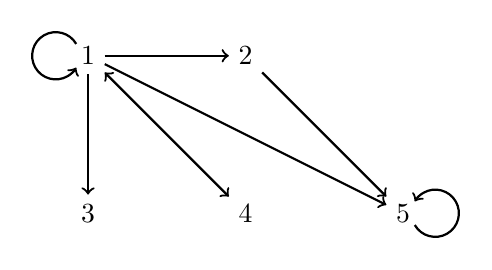
\begin{tikzpicture}
\node (atom1) at (0,2) {$1$};
\node (atom2) at (2,2) {$2$};
\node (atom4) at (0,0) {$3$};
\node (atom5) at (2,0) {$4$};
\node (atom6) at (4,0) {$5$};
\draw[->, thick] (atom1)+(-0.15,0.15) arc (-330:-30:.3); 
\draw[->, thick] (atom6)+(0.15,-0.15) arc (-150:150:.3); 
\draw[->, thick] (atom1) -- (atom2);
\draw[->, thick] (atom1) -- (atom4);
\draw[<->, thick] (atom1) -- (atom5);
\draw[->, thick] (atom1) -- (atom6);
\draw[->, thick] (atom2) -- (atom6);
\end{tikzpicture}
\end{center}
Determine whether each of the following sentences is true or false in that interpretation:
\begin{enumerate}
\item $\exists x\, \atom{R}{xx}$
\item $\forall x\, \atom{R}{xx}$
\item $\exists x \forall y\, \atom{R}{xy}$
\item $\exists x \forall y\, \atom{R}{yx}$
\item $\forall x \forall y \forall z ((\atom{R}{xy} \eand \atom{R}{yz}) \eif \atom{R}{xz})$
\item $\forall x \forall y \forall z ((\atom{R}{xy} \eand \atom{R}{xz}) \eif \atom{R}{yz})$
\item $\exists x \forall y\, \enot \atom{R}{xy}$
\item $\forall x(\exists y\, \atom{R}{xy} \eif \exists y\, \atom{R}{yx})$
\item $\exists x \exists y (\enot x = y \eand \atom{R}{x,y} \eand \atom{R}{yx})$
\item $\exists x \forall y(\atom{R}{xy} \eiff x = y)$
\item $\exists x \forall y(\atom{R}{yx} \eiff x = y)$
\item $\exists x \exists y(\enot x = y \eand \atom{R}{xy} \eand \forall z(\atom{R}{zx} \eiff y = z))$
\end{enumerate}
\problempart
Determine whether each of the following is valid or invalid, construct a proof if valid:
\begin{enumerate}
\item $\therefore \exists x (x = h \eand x = i)$
\item $\forall x(\atom{D}{x} \eif \exists y\, \atom{T}{yx}) \therefore \exists y \exists z\ \enot y= z$
\item $\enot \atom{R}{aa}$, $\forall x (x=a \eor \atom{R}{xa})$
\item $\forall x\forall y\forall z[(x=y \eor y=z )\eor x=z]$, $\exists x\exists y\ \enot x= y$
\item $\exists x\exists y((\atom{Z}{x} \eand \atom{Z}{y} )\eand x=y)$, $\enot \atom{Z}{d}$, $d=e$
\end{enumerate}



\chapter{Part 27 Equivalency Rules in QL}
\section{Part 27.1 The Equivalency Rules in PL are in QL}
As was previously mentioned, QL is an extension of PL. This means that not only do you have access to all of the inferences rules in PL but you also have access to all of the equivalency rules as well. Just like in PL, these rules can be applied to the main operator of a sentence (the entire sentence) or to just a part of it. it is worth remembering that equivalency rules are different from inference rules. Inference rules can only be done on the main operator and typically require two, or more, lines for the citation. Equivalency rules are basically when you are saying the same thing as before but in a different way (as I have mentioned). 

All that said, in QL, you can use Double Negation (DN), Commutativity (Comm), Material Conditional (MC), Biconditional Exchange (\eiff ex), DeMorgan's (DeM), and Tautology (TAUT). Below is a basic overview (refresher) of these rules and some examples of how they can be helpful in QL.

\subsection{DN and Comm}

Very often in QL, the main operator for a sentence will not be a connective like we had in PL, rather, it will be a quantifier. This means that when you are working with a complex sentence, you will need to use these equivalency rules. As with PL, Double Negation is the simplest; but you need to be careful that the two negations are right next to each other, nothing (not even a bracket) is between them. Double Negation is especially useful with the Quantifier Negation rule (next page). As a refresher, the rule looks like this: 
\factoidbox{
\enot \enot \metav{A} $\Leftrightarrow$ \metav{A}
}
'A' could be a simple or complex sentence and A could be the entire sentence or just a part. The major thing to remember is that the two negations are right beside each other. For example, this is not correct:
\begin{fitchproof}
\hypo{1}{\enot \exists x\enot Px}
\have{2}{\exists xPx}\by{naughty attempt to use DN}{1}
\end{fitchproof}
While it is true that, in this case, it is valid, there is a few missing steps of reasoning which you need to be aware of (through the Quantifier Negation rule). For a more egregious example of this sort of error, take a look at this: 
\begin{fitchproof}
\hypo{1}{\forall x\enot (\enot Px\eif Qx)}
\have{2}{\forall x(Px\eif Qx)}\by{naughty attempt to use DN}{1}	
\end{fitchproof}

The first line (1) is saying, roughly, that for anything, it's not the case that if it's not P, then it's Q or, in other words, everything is P and Q. The second line says something very different; namely, for anything, if it's P, then it's Q. 

Commutativity is another surprisingly useful rule in QL but it has it's caveats as well. To remind you, here are the different ways Comm can be used: 
\factoidbox{
(\metav{A}\eand \metav{B}) $\Leftrightarrow$ (\metav{B}\eand \metav{A})\\
(\metav{A}\eor \metav{B}) $\Leftrightarrow$ (\metav{B}\eor \metav{A})\\
(\metav{A}\eiff \metav{B}) $\Leftrightarrow$ (\metav{B}\eiff \metav{A})
}
When dealing with a sentence where the main operator is a conjunction, disjunction, or biconditional (those which are symmetric), you can flip the order without any worries. There is, however, one key, relatively common, error you need to be aware of:
\begin{fitchproof}
\hypo{1}{\forall x\exists yPxy}
\have{2}{\exists y\forall xPxy}\by{naughty attempt to use COMM}{1}	
\end{fitchproof}
 As you may recall, this is not a valid inference and these statements are not equivalent. The scope of the operators matters. You can avoid this sort of reasoning by being mindful of the fact that Comm only works in cases like those listed above. 

\subsection{MC and \eiff ex}

Material Conditional is very useful when dealing with negated conditionals (one of my favorite cases), but it is also useful when trying to work with mismatched consequents and antecedents.  Here are the cases where it can be used: 
\factoidbox{
(\metav{A}\eif \metav{B}) $\Leftrightarrow$ (\enot \metav{A}\eor \metav{B})\\
(\metav{A}\eor \metav{B}) $\Leftrightarrow$ (\enot \metav{A}\eif \metav{B})
}
This allows us to move between conditionals and disjunctions. There are not very many common errors or confusions with this one, but it is essential that you remember to tack-on the negation as required, even if there is one already there for example, in a case like this:
\begin{center}
(\enot A\eif B) \therefore  (\enot \enot A\eor B)
\end{center}
If your goal is actually A\eor B, then you can simply do a DN as an `additional' step. If you get comfortable skipping this DN step, you will be more prone to errors in your thinking in the future. 

Remember that \eiff ex is the one way we have to work with biconditionals. We need to use this step to derive things using biconditionals. Since biconditionals are conjoined conditionals, the rule looks like this: 
\factoidbox{
[(A\eif B)\eand (B\eif A)] $\Leftrightarrow$ (A\eiff B)
}
There are scant few errors made using this rule, but don't get too relaxed about it. For an example of how we can use this in QL, let's try this argument: 
\begin{center}
$\forall$ x(Px\eiff Qx) \therefore  $\forall$ x(Px\eif Qx)
\end{center}
This argument is valid, just like the QL version, here is the proof:
\begin{fitchproof}
\hypo{1}{\forall x(Px\eiff Qx)}
\have{2}{\forall x[(Px\eif Qx)\eand (Qx\eif Px)]}\by{\eiff ex}{1}
\have{3}{(Pa\eif Qa)\eand (Qa\eif Pa)}\Ae{2}
\have{4}{Pa\eif Qa}\ae{3}
\have{5}{\forall x(Px\eif Qx)}\Ai{4}
\end{fitchproof}
\subsection{DeM and TAUT}

DeMorgan's Law(s) are some of my personal favorites in Logic, and they are shockingly useful. As a reminder, DeMorgan's Law(s) essentially say that `neither X nor Y' means the same thing as `not-X and not-Y'. Similarly, they say that `not-X or not-Y' means the same as `not both X and Y'. This is symbolized like so: 
\factoidbox{
\enot (\metav{A}\eor \metav{B}) $\Leftrightarrow$ (\enot \metav{A}\eand \enot \metav{B})\\
\enot (\metav{A}\eand \metav{B}) $\Leftrightarrow$ (\enot \metav{A}\eor \enot \metav{B})
}
Like with Double Negation, it is good to remember that there can't be anything between the negation and the sentence with one of these main operators. For example, here is a naughty attempt: 
\begin{fitchproof}
\hypo{1}{\enot \forall x(Px\eor Qx)}
\have{2}{\forall x(\enot Px\eand \enot Qx)}\by{naughty attempt to use DeM}{1}	
\end{fitchproof}
The first line is saying, essentially, that something (at least one thing) is neither P nor Q while the second line is saying that everything is neither P nor Q. Those are very different statements. 

Tautology, as an equivalency rule not a kind of statement, comes in handy more often that you would think. We normally gloss over this in our reasoning but it is worthwhile to remember that errors happen when we aren't paying attention. TAUT works like this:
\factoidbox{
(\metav{A}\eor \metav{A}) $\Leftrightarrow$ (\metav{A})\\
(\metav{A}\eand \metav{A}) $\Leftrightarrow$ (\metav{A})
}
To see this equivalency rule at work in QL, take a look at this argument:
\begin{center}
$\forall$ x(Px\eif (Qx\eand Qx)),$\forall$ x(Qx\eif \enot Px) \therefore  $\forall$ x\enot Px
\end{center}
And here is the proof:
\begin{fitchproof}
\hypo{1}{\forall x(Px\eif (Qx\eand Qx))}
\hypo{2}{\forall x(Qx\eif \enot Px)}
\have{3}{\forall x(Px\eif Qx)}\by{TAUT}{1}
\have{4}{Pa\eif Qa}\Ae{3}
\have{5}{Qa\eif \enot Pa	}\Ae{2}
\have{6}{Pa\eif \enot Pa}\hs{4,5}
\have{7}{\enot Pa\eor \enot Pa}\mc{6}
\have{8}{\enot Pa}\by{TAUT}{7}
\have{9}{\forall x\enot Px}\Ai{8}	
\end{fitchproof}

We conclude here with everything isn't P. 
\section{Part 27.2 Change of Quantifier (Quantifier Negation)}
When we are symbolizing statements into QL, it should be noted that \enot $\forall$ x\enot Ax is logically equivalent to $\exists$ xAx and this makes sense. For example, if I say "it's not the case that everything isn't purple", this is just a long-winded way of saying that "something is purple". Similarly, \enot $\exists$ x\enot Ax is equivalent to $\forall$ xAx, and this too makes sense; if I say "it's not the case that someone isn't happy", this is, again, a long winded way of saying that "everyone is happy." In QL, these are actually provably equivalent, but it is a rather gruesome, involved proof. If you would like, for an added exersize, try to prove the following:
\begin{earg}
\item[]\enot $\forall$ x\enot Ax \therefore  $\exists$ xAx
\item[]\enot $\exists$ x\enot Ax \therefore  $\forall$ xAx
\item[]$\forall$ x\enot Ax \therefore  \enot $\exists$ xAx
\item[]$\exists$ x\enot Ax \therefore  \enot $\forall$ xAx
\end{earg}
Since the proofs for these are very involved and it would become very tiresome to need to run through the proofs every time you wanted to switch between these (when they are logically equivalent), we have given you a simple rule of equivalence, called Quantifier Negation (QN):
\factoidbox{
$\exists$ x\enot Ax $\Leftrightarrow$ \enot $\forall$ xAx\\
$\forall$ x\enot Ax $\Leftrightarrow$ \enot $\exists$ xAx
}
As a reminder, the `$\Leftrightarrow$' means that you can switch between these (the rule goes both ways) and the rule is an equivalency rule, meaning that it can be used in anywhere, even when it is not the main operator. One way to metaphorically think about this is that the negation is a snake and when it climbs over the quantifier, the snake flips it, from $\exists$  to $\forall$  or from $\forall$  to $\exists$  and then falls asleep on the other side. To see this in action, let's return to my favorite example for equivalency rules, now in QL rather than PL:
\begin{center}
\enot $\forall$ x(Ux\eif \enot Hx) \therefore  $\exists$ x(Ux\eand Hx)
\end{center}
In principle, we could read this as "it's not the case that for any x you pick, if x is a unicorn, then x doesn't have a horn. Therefore, there is an x such that x is a unicorn and x has a horn.". This might seem rather funny, but it is a perfectly valid argument and one which we can prove using all of the equivalency rules at our disposal:
\begin{fitchproof}
\hypo{1}{\enot \forall x(Ux\eif \enot Hx)}
\have{2}{ \enot \forall x(\enot Ux\eor \enot Hx)} \by{MC}{1}
\have{3}{\exists x\enot (\enot Ux\eor \enot Hx)}\by{QN}{2}
\have{4}{\exists x(\enot \enot Ux\eand \enot \enot Hx)}\by{DeM}{3}
\have{5}{\exists x(Ux\eand \enot \enot Hx)}\by{DN}{4}
\have{6}{\exists x(Ux\eand Hx)}\by{DN}{5}	
\end{fitchproof}
You might now be thinking "what about `\enot $\forall$ x\enot' and `\enot $\exists$ x\enot`? How can I use those?" Well, you need to remember that DN is allowed in QL, so, when you have something like \enot $\forall$ x\enot Px and you want $\exists$ xPx, just follow these steps, so something like them:
\begin{fitchproof}
\hypo{1}{\enot \forall x\enot Px}
\have{2}{\exists x\enot \enot Px}\by{QN}{1}
\have{3}{\exists xPx}\by{DN}{2}	
\end{fitchproof}
These steps can be done on something contained in a sentence or on the main operator. They are both equivalency rules, after all. Similarly, if you want to go from \enot $\exists$ x\enot Px to $\forall$ xPx, you need to follow similar steps:
\begin{fitchproof}
\hypo{1}{\enot \exists x\enot Px}
\have{2}{\forall x\enot \enot Px}\by{QN}{1}
\have{3}{\forall xPx}\by{DN}{2}	
\end{fitchproof}

Personally, I prefer having the negation move inward in the sentence when dealing with cases like this, but this is exclusively a matter of preference, there is nothing against doing these steps like this: 
\begin{fitchproof}
\hypo{1}{\enot \forall x\enot Px}
\have{2}{\enot \enot \exists xPx}\by{QN}{1}
\have{3}{\exists xPx}\by{DN}{2}	
\end{fitchproof}

Or like this:
\begin{fitchproof}
\hypo{1}{\enot \exists x\enot Px}
\have{2}{\enot \enot \forall xPx}\by{QN}{1}
\have{3}{\forall xPx}\by{DN}{2}	
\end{fitchproof}

\barcan

\practiceproblems
\problempart
Use the strategies to find proofs for each of the following arguments and theorems:
\begin{enumerate}
\item $A \eif \forall x\,\atom{B}{x} \therefore \forall x(A \eif \atom{B}{x})$
\item $\exists x(A \eif \atom{B}{x}) \therefore A \eif \exists x\, \atom{B}{x}$
\item $\forall x(\atom{A}{x} \eand \atom{B}{x}) \eiff (\forall x\,\atom{A}{x} \eand \forall x\,\atom{B}{x})$
\item $\exists x(\atom{A}{x} \eor \atom{B}{x}) \eiff (\exists x\,\atom{A}{x} \eor \exists x\,\atom{B}{x})$
\item $A \eor \forall x\,\atom{B}{x}) \therefore \forall x(A \eor \atom{B}{x})$
\item $\forall x(\atom{A}{x} \eif B) \therefore \exists x\,\atom{A}{x} \eif B$
\item $\exists x(\atom{A}{x} \eif B) \therefore \forall x\,\atom{A}{x} \eif B$
\item $\forall x(\atom{A}{x} \eif \exists y\,\atom{A}{y})$
\end{enumerate}
Use only the basic rules of QL in addition to the basic quantifier rules.

\problempart
Use the strategies to find proofs for each of the following arguments and theorems:
\begin{enumerate}
\item $\forall x\,\atom{R}{xx} \therefore \forall x\,\exists y\,\atom{R}{xy}$
\item $\forall x\,\forall y\,\forall z[(\atom{R}{xy} \eand \atom{R}{y,z}) \eif \atom{R}{xz}]$ \\
$\therefore \forall x\,\forall y[\atom{R}{xy} \eif \forall z(\atom{R}{yz} \eif \atom{R}{xz})]$
\item $\forall x\,\forall y\,\forall z[(\atom{R}{xy} \eand \atom{R}{yz}) \eif \atom{R}{xz}],$\\ $\forall x\,\forall y(\atom{R}{xy} \eif \atom{R}{yx})$ \\ $\therefore \forall x\,\forall y\,\forall z[(\atom{R}{xy} \eand \atom{R}{xz}) \eif \atom{R}{yz}]$
\item $\forall x\,\forall y(\atom{R}{xy} \eif \atom{R}{yx})$ \\$\therefore \forall x\,\forall y\,\forall z[(\atom{R}{xy} \eand \atom{R}{xz}) \eif \exists u(\atom{R}{yu} \eand \atom{R}{zu})]$
\item $\enot \exists x\,\forall y (\atom{A}{xy} \eiff \lnot\atom{A}{yy})$
\end{enumerate}

\problempart
Use the strategies to find proofs for each of the following arguments and theorems:
\begin{enumerate}
\item $\forall x\,\atom{A}{x} \eif B \therefore \exists x(\atom{A}{x} \eif B)$
\item $A \eif \exists x\, \atom{B}{x} \therefore \exists x(A \eif \atom{B}{x})$
\item $\forall x(A \eor \atom{B}{x}) \therefore A \eor \forall x\,\atom{B}{x})$
\item $\exists x(\atom{A}{x} \eif \forall y\,\atom{A}{y})$
\item $\exists x(\exists y\,\atom{A}{y} \eif \atom{A}{x})$
\end{enumerate}

\part{Modal Logic}
\label{ch.ml1}
\addtocontents{toc}{\protect\mbox{}\protect\hrulefill\par}
\stepcounter{chapcount}\setcounter{seccount}{1}
\chapter{Part \thechapcount: Introduction to Modal Logic}
\section{Part \thechapcount.\theseccount: What Is Modal Logic?}\stepcounter{seccount}
In both Propositional Logic and Quantified Logic, we have been dealing with sentences which are either true or false, we haven't had the ability to handle sentences which \emph{could} be true or which are \emph{possibly} false. Words or phrases which change the certainty of a simple sentence are called \glspl{modal}. There are many different modals in English and some other languages have more, less, or even entire verb conjugations which handle the different ways in which a sentence could be true. For example, consider these three English sentences:

\setcounter{Example}{0}
\begin{earg}
	\item[\ex{modal1}] Mac ate the cookie.
	\item[\ex{modal2}] Mac possibly ate the cookie.
	\item[\ex{modal3}] Mac necessarily ate the cookie. 
\end{earg}

These three sentences are saying radically different things. They all concern whether Mac ate the cookie, but they differ in the scope of the truth of that fact.  In sentence \ref{modal1}, this is restricted merely to the actual world. There is nothing special going on, just that Mac ate the cookie. Sentence \ref{modal2} is different, however. Adding the adverb `possibly' to the sentence changed the scope or range of the sentence. Rather than saying something definite, like sentence \ref{modal1}, this sentence has some wiggle room. All it is saying is that Mac \emph{could have} eaten the cookie, there is a concievable scenario where Mac did eat the cookie but we do not know whether that scenario was actual. This is significantly weaker than sentence \ref{modal1}. Sentence \ref{modal3}, on the other hand, uses the phrase `necessarily'. This is significantly stronger than sentences \ref{modal1} and \ref{modal2}. This sentence doesn't leave any wiggle room, it is saying that in every single relevant possible scenario, Mac ate the cookie. It is making this claim with a level of certainty not had in the other two sentences. 

Neither PL nor QL has the ability to accurately handle sentences like these. With PL, they would be symbolized as three different simple sentences and the fundamental logical connection between them, had because of the form, would be irretrievably lost. For QL, the connection that all three concern Mac would be preserved but the predicates would be radically different and, again, the formal link connecting them would be lost. Similarly, for both PL and QL, various seemingly valid inferences concerning the nature of possibility and necessity would be judged invalid because neither has the capability to reason in this way. This is why we need a different logical system.

Modal logic (ML) is the logic of modalities, ways in which a statement can be true. Necessity and possibility are two such modalities: a statement can be true, but it can also be necessarily true (true no matter how the world might have been). For instance, logical truths are not just true because of some accidental feature of the world, but true come what may. A possible statement may not actually be true, but it might have been true. ML starts off, much like QL, as an expansion of PL, but rather than adding \emph{quantifiers}, ML incorporates \glspl{qualifier} in order to represent different modalities and give a formal structure for reasoning with or about them. Quantifiers, as the name implies, give information about the amount, the \emph{quantity}, of things which have some feature(s). Qualifiers, on the other hand, \emph{qualify}, or restrict/expand, the truth of the statements. 

\newglossaryentry{modal}
{
name=modal,
description={A word or phrase such as ``possibly'' or ``necessarily'' which qualifies, restricts or gives caveats to, the truth of the sentence in question},
plural=modals
}

\newglossaryentry{qualifier}
{
name=qualifier,
description={A logical operator which specifies the \gls{modal} in a sentence},
plural=qualifiers
}

As a brief introduction to this family of logics, we use `\ebox' to express necessity, and `\ediamond' to express possibility. So you can read \ebox A as `It is necessarily the case that A', and \ediamond A as `It is possibly the case that A'. It should be noted that there are many different kinds of possibility and necessity. For example, it is not humanly possible for me to run at 100mph but it is physically possible for a person to run that fast (replace my legs with a robot's). Similarly, it is not physically possible to move faster then the speed of light, but doing so is logically possible. 

ML has the power to handle all of them. We can use it in some contexts for logical possibility, in another physical possibility, in another practical possibility, and in yet another human possibility. They all work using the same rules, we just need to specify the range of scenarios we are deeming possible in the context. ML is a very flexible tool.

In fact, ML is so flexible that we don't necessarily need to think of `\ebox'  and `\ediamond'  as expressing necessity and possibility. Doxastic Logic is a branch of ML which deals with beliefs and knowledge. They think of `\ediamond'  as `S believes...' and `\ebox'  as `S knows...'. So, for example, using the same logical rules and operations as ML, Doxastic Logic can prove arguments like:
\begin{earg}
\item[]S knows that P and knows that if P is true, then M is true. 
\item[\therefore] S knows M. 
\end{earg}
Another example is  Deontic Logic which deals with moral obligations and permissibility. For this one, we think of `\ebox' as `it is obligatory that...' (doing otherwise is morally wrong, we have a moral obligation to do it) and `\ediamond'  as `it is permissible that...' (doing it is morally fine/OK). Just as before, using the same general rules found in ML, Deontic Logic be used to prove arguments like:
\begin{earg}
\item[]C is permissible and if C is the case, then P is. 
\item[\therefore] P is also permissible. 
\end{earg}
Both of these, and a litany of others all boil down to different interpretations and applications of these two operators, `\ebox'  and `\ediamond', though they tend to use different ones to save confusion.

A modal formula is one that includes qualifiers such as `\ebox' and `\ediamond'. Depending on the interpretation we assign to `\ebox' and `\ediamond', different modal formulae will be provable or valid from a set of premises or none at all. These interpretations, in a sense, tell us the system we are working in, what sort of logical moves are allowed. For instance, \ebox A \eif A might say that “if A is necessary, it is true,” if `\ebox'  is interpreted as necessity. It might express “if A is known, then it is true,” if `\ebox'  expresses known truth. Under both these interpretations, \ebox A\eif A is valid: All necessary propositions are true in any scenario, so are true in the actual one. And if a proposition is known to be true, it must be true (one can’t know something that’s false). However, when `\ebox'  is interpreted as “it ought to be the case that,” then \ebox A \eif A is not valid. For example, if we interpret `A' to mean “Every murderer will be brought to justice.” We should hold that this ought to be true, but sadly it isn't.

We will consider different kinds of systems of ML. They differ in the rules of proof allowed and in the semantics we use to define our logical notions. Logicians have reduced the various different possible models or structures which we can reason in down to six generic systems. Here, we will consider four of them, namely: K, T, S4, and S5. 

K is the basic system; everything that is valid or provable in K is also provable in the others. But there are some things that K does not prove, such as the formula \ebox A \eif A for sentence letter A. So K is not an appropriate modal logic for necessity and possibility (where \ebox A \eif A should be provable). But it may be appropriate for moral reasoning (Deontic Logic), as we do not want, for example, to be able to move from A to \ediamond A (it is the case that A to it's permissible that A). These general moves are allowed and provable in the T system, making it appropriate for cases where such moves are reasonable. T, however, cannot handle all of the different reasonable formal moves which we have access to when dealing with possibility and necessity, S4 can handle most of it and S5 can handle all of it.  
\section{Part 28.2 The Language of ML}
In order to do modal logic, we have to do two things. First, we want to see how to construct interpretations for ML. Second, we want to learn how to prove things in ML. The interpretations, like with QL, are used to prove invalidity and are essential to understanding where the various logical rules come from; so you can see which ones are allowed in your given context. But before we can do either of these things, we need to explain how to construct sentences in ML.

The language of ML is an extension of PL. We could have started with QL, which would have given us Modal Quantified Logic (MQL). MQL is much more powerful than ML, but it is also much, much more complicated and contentious (there is a substantial amount of debate over the range of the domains in MQL which has a great deal of sway over which inference rules are allowed). So we are going to keep things simple, and start with PL.

Just like PL, ML starts with an infinite stock of atoms. These are written as capital letters, with or without numerical subscripts: A, B, \ldots,$ A_1, B_1$,\ldots We then take all of the rules about how to make sentences from PL, and add two more for \ebox  and \ediamond :
\factoidbox{\begin{enumerate}\label{langofml}
\item Every atom of ML is a sentence of ML.
\item If \metav{A} is a sentence of ML, then \enot \metav{A} is a sentence of ML.
\item If \metav{A} and \metav{B} are sentences of ML, then (\metav{A}\eand \metav{B}) is a sentence of ML.
\item If \metav{A} and \metav{B} are sentences of ML, then (\metav{A}\eor \metav{B}) is a sentence of ML.
\item If \metav{A} and \metav{B} are sentences of ML, then (\metav{A} \eif  \metav{B}) is a sentence of ML.
\item If \metav{A} and \metav{B} are sentences of ML, then (\metav{A} \eiff  \metav{B}) is a sentence of ML. 
\item If \metav{A} is a sentence of ML, then \ebox \metav{A} is a sentence of ML.
\item If \metav{A} is a sentence of ML, then \ediamond \metav{A} is a sentence of ML.
\item Nothing else is a sentence of ML.
\end{enumerate}}
Here are some examples of ML sentences:
\begin{center}
A, P \eor  Q, \ebox A, C \eor  \ebox D, \ebox \ebox (A \eif  R), \ebox \ediamond (S \eand  (Z \eiff  (\ebox W \eor  \ediamond Q)))
\end{center}
\practiceproblems
\problempart
Using the following symbolization key, symbolize the following sentences and arguments into ML:
	\begin{ekey}
		\item[M] Max goes to the party
		\item[S] Sally is happy
		\item[J] Jack goes up the hill
		\item[F] Jill follows Jack
		\item[P] John will be at the party
		\item[K] Kirito is heroic
		\item[A] Asuna loves Kirito
		\item[V] Video games are healthy
		\item[C] Cigarettes are healthy
		\item[R] Rika is jealous
	\end{ekey}

\begin{enumerate}
\item Necessarily, Cigarettes are unhealthy only if video games are. Cigarettes are, in fact, unhealthy. Therefore, video games possibly are unhealthy.
\item If Jack goes up the hill, Jill will follow him. Jill isn't following him. Therefore, Jack isn't going up the hill.
\item If Asuna possibly loves Kirito, Rika is jealous. If Kirito is heroic, then Asuna loves him. Kirito possibly is heroic. Therefore, Rika is jealous. 
\item Necessaily, Jack will go up the hill unless Jill doesn't follow him. Jill is following Jack. Therefore, Jack will go up the hill.
\item If Sally is happy, then Rika is jealous. If Max goes to the party, then Rika will be jealous. Sally won't be happy unless Max goes to the party. Therefore, Rika is going to be jealous.
\item John will be at the party if and only if both cigarettes and video games are healthy. Neither cigarettes nor video games are healthy. Therefore, John will not be at the party. 
\item Max is going to the party if Jack goes up the hill. Either Jack won't go up the hill or Sally is happy. Therefore, if Jack goes up the hill then both Max goes to the party and Sally is happy.
\item If John will be at the party, then Jack will go up the hill. If Jack goes up the hill, then Jill will follow him. If Jill follows him, then Rika will be jealous. Therefore, if John will be at the party, then Rika will be jealous. 
\item Asuna loves Kirito if and only if both she loves him and he is heroic. He is heroic only if video games are unhealthy. Therefore, Asuna loves Kirito only if video games are unhealthy. 
\end{enumerate}

\problempart
Give a symbolization key and symbolize the following English sentences in ML:
\begin{enumerate}
\item Possibly, Alice and Bob are both spies.
\item Necessarily, if either Alice or Bob is a spy, then the code has been broken.
\item If neither Alice nor Bob is a spy, then the code remains unbroken.
\item The German embassy will be in an uproar, unless someone has broken the code.
\item Either the code has been broken or it has not, but the German embassy will be in an uproar regardless.
\item Either Alice or Bob is a spy, but not both.
\item If there is food to be found in the pridelands, then Rafiki will talk about squashed bananas.
\item Rafiki will talk about squashed bananas unless Simba is alive.
\item Rafiki will either talk about squashed bananas or he won't, but there is food to be found in the pridelands regardless.
\item Scar will remain as king if and only if there is food to be found in the pridelands.
\item If Simba is alive, then Scar will not remain as king.
\end{enumerate}

\problempart
Symbolize the following arguments. A symbolization key is not provided, so you will need to make one yourself for each argument. Some of these arguments are, in fact, invalid. You may return to these as extra practice problems within the next module.
\begin{enumerate}
\item If Tristen is driving, then he is going to work. If he is texting, then he is goofing off. Therefore, if Tristen is both texting and driving, then he is both going to work and goofing off.
\item The car gets 30 miles to the gallon. If Joe can get to the gas station, then the car gets 30 miles per gallon. Therefore, Joe can get to the gas station.
\item The car gets 30 miles to the gallon. If the car gets 30 miles per gallon, then Joe can get to the gas station. Therefore, Joe can get to the gas station.
\item If Dorothy plays the piano in the morning, then Roger wakes up cranky. Dorothy plays piano in the morning unless she is distracted. So if Roger does not wake up cranky, then Dorothy must be distracted.
\item It will either rain or snow on Tuesday. If it rains, Neville will be sad. If it snows, Neville will be cold. Therefore, Neville will either be sad or cold on Tuesday.
\item If Zoog remembered to do his chores, then things are clean but not neat. If he forgot, then things are neat but not clean. Therefore, things are either neat or clean; but not both.
\end{enumerate}
\stepcounter{chapcount}\setcounter{seccount}{1}
\chapter{Part \thechapcount: The Systems of Modal Logic}
Now that we know how to make sentences in ML, we can look at how one can make interpretations (models), countermodels, and proofs in ML. We will use $\vDash$  to express provability/validity (if it is provable in these systems, then it is valid), just like how we did in PL. So $A_1,A_2,\ldots A_n$ $\vDash$  C means that C can be proven from $A_1,A_2,\ldots A_n$. There are many different applications of ML which we may want to consider and these different applications allow for different inference rules. As mentioned previously, \ebox A $\vDash$ A is just fine if we are working in the T system but it is not if we are working in the more basic K system. We will be looking at a number of these `systems' of ML, and so it will be useful to add a subscript to indicate which system we are working with. So for example, if we want to say that we can prove C from $A_1,A_2,\ldots A_n$ in system K, we will write: $A_1,A_2,\ldots A_n$ $\vDash_K$ C.

\section{Part \thechapcount.\theseccount: But what are these systems?}\label{ml.systems}\stepcounter{seccount}

Imagine, if you will, a world consisting of an arbitrary number of insular (island) micro-nations. These nations could wish to set up any number of different trading networks between them, either internally or with other nations or both. Sometimes, all of the nations will have a product similar (for example, all of the nations could grow oranges), other times, there may be products which one island has (or a few islands have) but not all of them do. The different sorts of trading relations these nations have between each other (or internally) represent, on an abstract level, the different systems which ML could be using in a given context or argument. Just for the sake of explanation, we will say that there aren't any laws or the like forbidding a product from being traded once a trade route (either internal or international) is established. For example, suppose that we have a world where there are only two insular nations within trading distance of each other, one of them ($w_1$) has P while the other ($w_2$) has Q. We might diagram (\gls{model}) a trading relationship between them like so, with the arrows representing the `accessibility' of the products (meaning that if an arrow is going from $w_1$ to $w_2$, then $w_1$ has access to the products in $w_2$):\\
\begin{center}
\begin{tikzpicture}[modal]
		\node[world] (w1) [label=left:$w_1$] {P};
		\node[world] (w2) [label=right:$w_2$, right=of w1]{Q};
		%\path[->] (w2) edge[reflexive above] (w2);
		\path[->] (w1) edge (w2);
	\end{tikzpicture}
\end{center}
\begin{itemize}
\item[W:] $w_1,w_2$
\item[R:]$\openntuple w_1,w_2\closentuple$  
\item[$w_1$:] P,...
\item[$w_2$:] Q,...
\end{itemize}
   
 \newglossaryentry{model}
{
name={model},
text={model},
description={In Modal Logic, this is a list of worlds, an assignment of accessibility relations between those worlds, and an assignment of the sentences true at those worlds. This is represented as either a diagram or as an interpretation like in QL}
}
  
Using this diagram, we can say that $w_1$ has access to the products in $w_2$ but there isn't an arrow from $w_1$ to $w_1$ (an arrow curling back), so $w_1$ doesn't have internal trading. In ML, these `island nations' are called \glspl{world} and the different `trade routes' between them are called the \glspl{accessibility relation}. You may notice that I have given an interpretation for the diagram above. This is because, at least formally, the models in ML are very similar to the interpretations in QL. We can, and do, describe the different models for the worlds and accessibility relations in a very similar way to how we directly stipulated the extension of a two-place predicate for interpretations in QL. W is the list of worlds in the `universe' we wish to consider; this is similar to the `domain' in QL. The two-place relational predicate for the accessibility relation is called \gls{R}; which we treat like a relational predicate in QL, though it is `meta' to QL. From here, there is a minor difference/expansion. The worlds are not treated like names in QL, rather they are treated as sets of jointly possible sentences all of which are true at that world. These could be simple sentences, like A, $A_1$, $A_2$... $P_1$, Q, Y,... $Z_{98022}$,  or they could be complex sentences like $P\eif Q$ or $(A\eor B)\eand(A\eif C)$.\footnote{For these simple example diagrams, I am using simple sentences. In general, you should only need to list the simple sentences which are true at the world in question, but more complex sentences may be included if necessary to make the model.} As a result, for each world, we will need to include a list of the sentences which are true at that world.  

\newglossaryentry{world}
{
name=world,
description={A set jointly satisfiable sentences. You can also think of them as possible scenarios or `ways the world could have been'},
plural=worlds
}

\newglossaryentry{accessibility relation}
{
name=accessibility relation,
description={A relation between \glspl{world} such that one has access to the other; that is, the world is possible from their perspective},
plural=accessibility relations
}

\newglossaryentry{R}
{
name=R,
description={The two place predicate used to define the \gls{accessibility relation} between \glspl{world}}
}


For this simple example, I am merely using one simple sentence in each world, but most of the time, there will be many. You can use this means of directly stipulating the relations and content of an interpretation to give counter examples and prove invalidity withing ML as well, especially when it would be too cumbersome to draw all of the relations and worlds as a diagram. Using models like this, we can define what it means for a statement to be possibly true and for a statement to be necessarily true like so:
\factoidbox{
In a model, \ediamond \metav{A} is true at some world ($w_1$) if and only if there is some other world, $w_2$, such that \metav{A} is true at $w_2$ and $w_2$ is accessible to $w_1$ (meaning that there is an arrow pointing from $w_1$ to $w_2$).\\
In a model, \ebox \metav{A} is true at some world ($w_1$) if and only if for all worlds such that $w_1$ has access to them, \metav{A} is true at those worlds.
}
Notice that I said `at some world', this is because in ML the truth of a sentence is relative to the world you are in. When you are doing proofs in ML, there is an assumed `actual world', often given a special label in the models like \metav{a} rather than simply `w' with a subscript number. The truth of the different modal statements is determined by the relation to the `actual world'. So, in this model, \ediamond Q is true at $w_1$. Similarly, since $w_1$ only has access to one other world and Q is true at that world, \ebox Q is also true at $w_1$. But, R$w_1$$w_1$ is not true in the above interpretation and P is true at any of the worlds $w_1$ can `see', so \ediamond P is not true at $w_1$.

Since the accessibility relation, R, is a relational predicate, R could have the four general features which we have seen previously (see \nameref{ss.featuresmanyplaced}). The different systems of Modal Logic all relate to whether R has a feature or lacks it.  Each of these four features give us different valid inference rules which we could use if the system has the feature. Here is a quick overview of the four, which I will go over in more detail, we also covered this previously:
\factoidbox{
\begin{earg}
\item[]R is \gls{serial} if and only if for every world x, there is a world y such that Rxy.
\item[]R is \gls{reflexive} if and only if for any world w, Rww.
\item[]R is \gls{symmetric} if and only if for any world x and for any world y, if Rxy, then Ryx.
\item[]R is \gls{transitive} if and only if for any x, for any y, and for any z, if Rxy and Ryz, then Rxz.
\end{earg}}
\subsection{Serial}

Relating back to our trading relations, if every nation has access to the products in some nation (may be another or it may be the same nation), then the R relation in that model is \gls{serial}. For example, the example I gave above is not serial because $w_2$ doesn't have access to any products, not even internal trading is allowed. To make it serial, all we need to do is make it so that $w_2$ has access to its own products, so to speak, or that it can `see' itself:


\newglossaryentry{serial}
{
name=serial,
description={A property had by a relation R such that for any x you pick, there is a y such that Rxy. In other words, R is serial if and only if everything has that relation to something (maybe itself)}
}

\begin{center}
	\begin{tikzpicture}[modal]
		\node[world] (w1) [label=left:$w_1$] {P};
		\node[world] (w2) [label=right:$w_2$, right=of w1]{Q};
		\path[->] (w2) edge[reflexive above] (w2);
		\path[->] (w1) edge (w2);
	\end{tikzpicture}
\end{center}
\begin{itemize}
\item[W:] $w_1,w_2$
\item[R:]$\openntuple w_1,w_2\closentuple$,$\openntuple w_2,w_2\closentuple$  
\item[$w_1$:] P,...
\item[$w_2$:] Q,...
\end{itemize}
   
Now, $w_2$ has access to its own products, so to speak, so the R relation for this model is serial as every world has access to products. There are many other ways in which this could be done and being serial is the lowest bar one needs to cross. Just about any context where you would want to employ the tools from ML will be serial. In QL, some relational predicates could have been serial as well (see \nameref{sss.serial}). There, a relational predicate, L, is serial if and only if $\forall x \exists y Lxy$. For a Modal Logic system, the accessibility relation, R, is serial if and only if for any world, $w_1$, there is a world, $w_2$, such that R$w_1$$w_2$. But, it is worth noting that just like in QL one cannot assume that everything bears the relation to themselves, you cannot move from  $\forall x \exists y Lxy$ to  $\forall x  Lxx$. There is another feature, reflexivity, which allows for this kind of move. 

\subsection{Reflexive}

A simple way to remember this is that the word `\gls{reflexive}' looks and sounds a lot like the word `reflective', this is to say, roughly, that all of the worlds can see themselves. Using the trading analogy, this says that all of the nations allow for internal trading. The simplest case for a reflexive system is one with only one world and one relation, it can see itself, like so:

\begin{center}
	\begin{tikzpicture}[modal]
		\node[world] (w1) [label=left:$w_1$] {P};
		\path[->] (w1) edge[reflexive above] (w1);
	\end{tikzpicture}
\end{center}
\begin{itemize}
\item[W:] $w_1$
\item[R:]$\openntuple w_1,w_1\closentuple$ 
\item[$w_1$:] P,...
%\item[$w_2$:] Q,...
\end{itemize}


A minimalist case like this is hardly useful, but it is possible and one which we need to consider for validity and provability in some systems. A more practical model would be based on the previous model used to illustrate being serial. That model did not have this feature because $w_1$ could not `trade' or `see' with itself. If someone in this nation wanted to get a product, they would need to get it from $w_2$, they can't get anything locally, sadly. Reflexivity is easily added to that model:


\begin{center}
	\begin{tikzpicture}[modal]
		\node[world] (w1) [label=left:$w_1$] {P};
		\node[world] (w2) [label=right:$w_2$, right=of w1]{Q};
		\path[->] (w1) edge[reflexive above] (w1);
		\path[->] (w2) edge[reflexive above] (w2);
		\path[->] (w1) edge (w2);
	\end{tikzpicture}
\end{center}
\begin{itemize}
\item[W:] $w_1,w_2$
\item[R:]$\openntuple w_1,w_1\closentuple$,$\openntuple w_2,w_2\closentuple$,$\openntuple w_1,w_2\closentuple$  
\item[$w_1$:] P,...
\item[$w_2$:] Q,...
\end{itemize}
 
 
\newglossaryentry{reflexive}
{
name=reflexive,
description={A property had by a relation R such that for any x you pick Rxx. In other words, R is reflexive if and only if everything has that relation to itself}
}
\subsection{Symmetric}

One way to think of this is in terms of symmetry, like in art. The accessibility relations are \gls{symmetric} when they go both ways. This, again, is the same as one of the features relational predicates could have (see \nameref{sss.symmetric}). In QL, a relational predicate, L, is symmetric if and only if $\forall x \forall y (Lxy \eif Lyx)$. Here, we can say something similar, for some Modal Logic system, the accessibility relation, R, is symmetric if and only if for any worlds $w_1$ and $w_2$, if R$w_1$$w_2$, then R$w_2$$w_1$.  If I can see you, then you can see me. You might be thinking in our model, that $w_2$ is getting the bad end of the trade deals, $w_1$ has access to all of their products but they don't have access to any of $w_1$'s products. If we made the accessibility relation symmetric, this inequity goes away. The simplest diagram for this case is the same as the one for reflexive, but that is not all that explanatory, so another, very simple case looks like this:

\begin{center}
\begin{tikzpicture}[modal]
		\node[world] (w1) [label=left:$w_1$] {P};
		\node[world] (w2) [label=right:$w_2$, right=of w1]{Q};
		%\path[->] (w2) edge[reflexive above] (w2);
		\path[<->] (w1) edge (w2);
	\end{tikzpicture}
\end{center}
\begin{itemize}
\item[W:] $w_1,w_2$
\item[R:]$\openntuple w_1,w_2\closentuple$,$\openntuple w_2,w_1\closentuple$  
\item[$w_1$:] P,...
\item[$w_2$:] Q,...
\end{itemize}


 As you can see, with this model, the relation isn't just an arrow going one way, but it goes in both directions, this means that they can see each other or the trade relation is equal. This particular model, however, might lead you to make assumptions about how other models might look so here is a more complicated model which better illustrates this feature:
\begin{center}
	\begin{tikzpicture}[modal]
		\node[world] (w1) [label=left:$w_1$] {P};
		\node[world] (w2) [label=above:$w_2$, right=of w1]{Q};
		\node[world] (w3) [label=right:$w_3$, below=of w1]{R};
		\path[->] (w1) edge[reflexive above] (w1);
		\path[->] (w2) edge[reflexive right] (w2);
		\path[->] (w3) edge[reflexive left] (w3);
		\path[<->] (w1) edge (w2);
		\path[<->] (w1) edge (w3);
	\end{tikzpicture}
\end{center}
\begin{itemize}
\item[W:] $w_1,w_2,w_3$
\item[R:]$\openntuple w_1,w_1\closentuple$,$\openntuple w_2,w_2\closentuple$,$\openntuple w_3,w_3\closentuple$,$\openntuple w_1,w_2\closentuple$,$\openntuple w_2,w_1\closentuple$,$\openntuple w_1,w_3\closentuple$,$\openntuple w_3,w_1\closentuple$  
\item[$w_1$:] P,...
\item[$w_2$:] Q,...
\item[$w_3$:] R,...
\end{itemize}

\newglossaryentry{symmetric}
{
name=symmetric,
description={A property had by a relation R such that for any x you pick, for any y you pick if Rxy, then Ryx. In other words, R is symmetric if and only if all of relations go both ways.}
}

You will notice that this looks a lot like the one which we have been building up but I  I added another world to the diagram, $w_3$, and that this world does not have a connection with $w_2$. This is because symmetry only gives you that the relation goes in both directions, it does not get you that they could `skip the middle man'. From $w_3$'s perspective, \ediamond \ediamond Q is true, because \ediamond Q is true at $w_1$ but \ediamond Q is not true because they don't have access to a world where Q is true, so within this model, moving from possibly possibly Q to just possibly Q would not be allowed.

\subsection{Transitive}

The caveat I gave in the previous feature might not have sat well with you. You might have thought that the additional `possiblies' didn't add anything and that you could drop them. There are contexts in Modal Logic where this is a perfectly valid move, but the models which allow for this need, at the very least, a fourth and final feature; \glspl{transitive}. This sort of relationship should seem intuitive. If Bob is taller than Mac and Mac is taller than Dave, then Bob is taller than Dave. This was also a feature which relational predicates in QL could have (see \nameref{sss.transitive}). This particular feature allows you to, in a sense, skip the middle man. A relatively simple diagram for this case, which does not have any of the other features, looks like this:
\begin{center}
	\begin{tikzpicture}[modal]
		\node[world] (w1) [label=left:$w_1$] {P};
		\node[world] (w2) [label=above:$w_2$, right=of w1]{Q};
		\node[world] (w3) [label=right:$w_3$, right=of w2]{R};
		\path[->] (w1) edge (w2);
		\path[->] (w2) edge (w3);
		\path[->] (w1) edge[bend right] (w3);
	\end{tikzpicture}
\end{center}
\begin{itemize}
\item[W:] $w_1,w_2,w_3$
\item[R:]$\openntuple w_1,w_2\closentuple$,$\openntuple w_2,w_3\closentuple$,$\openntuple w_1,w_3\closentuple$
\item[$w_1$:] P,...
\item[$w_2$:] Q,...
\item[$w_3$:] R,...
\end{itemize}


\newglossaryentry{transitive}
{
name=transitive,
description={A property had by a relation R such that for any x y and z, if Rxy and Ryz, then Rxz. In other words, R is transitive if and only if the relation `bridges the gap' or can `cut out the middle man'.},
plural=transitivity
}

With this particular model, a system with only transitivity, we can move from \ediamond\ediamond\metav{A} to \ediamond\metav{A}. Without reflexivity, you can't drop the additional `\ebox', if there is one, but, if you incorporate the other features, like symmetry and reflexivity, we end up with a model like this:
\begin{center}
	\begin{tikzpicture}[modal]
		\node[world] (w1) [label=left:$w_1$] {P};
		\node[world] (w2) [label=right:$w_2$, right=of w1]{Q};
		\node[world] (w3) [label=right:$w_3$, below=of w1]{R};
		\path[->] (w1) edge[reflexive above] (w1);
		\path[->] (w2) edge[reflexive above] (w2);
		\path[->] (w3) edge[reflexive left] (w3);
		\path[<->] (w1) edge (w2);
		\path[<->] (w1) edge (w3);
		\path[<->] (w2) edge (w3);
	\end{tikzpicture}
\end{center}
\begin{itemize}
\item[W:] $w_1,w_2,w_3$
\item[R:]$\openntuple w_1,w_1\closentuple$,$\openntuple w_2,w_2\closentuple$,$\openntuple w_3,w_3\closentuple$,$\openntuple w_1,w_2\closentuple$,$\openntuple w_2,w_1\closentuple$,$\openntuple w_1,w_3\closentuple$,$\openntuple w_3,w_1\closentuple$,$\openntuple w_2,w_3\closentuple$,\\$\openntuple w_3,w_2\closentuple$  
\item[$w_1$:] P,...
\item[$w_2$:] Q,...
\item[$w_3$:] R,...
\end{itemize}

This model has all of the features in one. Models like this represent the most robust modal system, called S5, which is best for reasoning about logical possibility. There are others which do not have all of the features, and some might have none at all. But, if you know that the model you are working in has an R relation with a certain feature, then there are inference/equivalency rules which you may use depending on the feature had. S5, as it happens, gets all of them unrestricted. 

\section{Part \thechapcount.\theseccount: Modal Negation (The Equivalency Rule For Modal Logics)}\stepcounter{seccount}
In \nameref{ml.systems}, I laid out what the general features a Modal Logic system could have. Each of those different features imply different inference rules which one has at their disposal. Those rules, however, are not equivalency rules. Equivalency rules are based on the definitions of the operators (modals, quantifiers, connectives) in question. This means that if ML has a special equivalency rule, then it will work regardless of the system you are working in. Looking back at the section about what makes a \ediamond   statement true and what makes a \ebox   statement true, you might have noticed a similarity between these and the quantifiers in QL. This is not by chance, they are very similar. Because of this similarity, one could, in principle, define \ebox   and \ediamond   in relation to each other, much like how one could define $\forall$  and $\exists$  in relation to each other (see \nameref{s.QN}). For example:
\factoidbox{
$\forall$ x\metav{A} $=_{df}$ \enot $\exists$ x\enot \metav{A}\\
$\exists$ x\metav{A} $=_{df}$ \enot $\forall$ x\enot \metav{A}\\
\ediamond \metav{A} $=_{df}$ \enot \ebox \enot \metav{A}\\
\ebox \metav{A} $=_{df}$ \enot \ediamond \enot \metav{A}}

In other words, to say that A is possibly true, is to say that A is not necessarily false. This is akin to the meaning behind the quantifiers in QL, if everything is A, then nothing isn't A, As a result, it isn’t really essential to add a \ediamond . So, we can use this definition to give us some equivalency rules which will always be available to you, this is the Modal Negation Rule (MN), so named because of its similarity to the Quantifier Negation Rule:
\factoidbox{
\enot \ebox \metav{A} $\Leftrightarrow$  \ediamond \enot \metav{A}\\
\enot \ediamond \metav{A} $\Leftrightarrow$ \ebox \enot \metav{A}
}
In any system, one can use the Modal Negation Rule and Double Negation to prove \ediamond A \eiff  \enot \ebox \enot A. Similarly, you can prove \ebox A \eiff  \enot \ediamond \enot A. MN and DN are very useful in Modal Logics. Here are some different ways one can read this move, given different interpretations of the two qualifiers:
\factoidbox{
It is not necessary that A $\Leftrightarrow$  It is possible that A is false.\\
It is not possible that A is true $\Leftrightarrow$  It is necessary that A is false.\\
It's not the case that I know that A is true $\Leftrightarrow$  Given my evidence, A could be false.\\
It is not the case that given my evidence A is true $\Leftrightarrow$  I know that A is false.\\
It isn't an obligation to A $\Leftrightarrow$  it is permissible to not A.\\
It isn't permissible to A $\Leftrightarrow$  It is an obligation not to A (A is forbidden).\\
It is not the case that A always will be $\Leftrightarrow$  there is a future time where A isn't.\\
It's not the case that A will happen $\Leftrightarrow$  It will always be the case that A isn't.\\ 
A wasn't always the case $\Leftrightarrow$  there was a time when A wasn't.  \\
}
\section{Part \thechapcount.\theseccount: The K System}\stepcounter{seccount}
We start with a particularly simple system called \Gls{K}, in honor of the philosopher and logician Saul Kripke. Since ML is an expansion upon PL, all systems for Modal Logic will have all of the inference and equivalency rules found in PL and K is no different. K is special, however, because it does not have any requirements about the features the R relation might have. This means that any model or interpretation will count as a K model (a system using K). This also means that if an argument is valid in K (sometimes called K-valid), then it is valid in all other systems. Because there are no special features we can be certain R will have in a K-model, there is very little one can prove in it. The simplest example of a K-model looks like this:

\begin{center}
	\begin{tikzpicture}[modal]
		\node[world] (w1) [label=left:\metav{a}] {P};
	\end{tikzpicture}
\end{center}
\begin{itemize}
\item[W:] \metav{a}
\item[R:] 
\item[\metav{a}:] P,...
%\item[$w_2$:] Q,...
\end{itemize}

Notice that there are no other worlds except for \metav{a}, which we will use to mark the `actual world'. From \metav{a}'s perspective, nothing is possible because there are no possible worlds it has access to. Even in such a barren model, however, there are modal operations we can use. 

K has a very special kind of subproof (called a `strict subproof' or `SS' for short) and a few new basic rules for \ebox . These strict subproofs allow us to reason about alternative possibilities by, in a sense, moving into that alternative possibility. We are changing our focus from the actual world to a possible world, working inside of it, and then exporting conclusions back to the actual world (with the appropriate qualifier). The strict subproofs look like ordinary subproofs, but it has a very special caveat; all assumptions are disregarded, and we are not allowed to appeal to any lines outside the strict subproof (except as allowed by the modal rules given later). Different systems allow for us to import different assumptions into the strict subproof, so as we add more features to R, what we can prove increases.

\kripke

\newglossaryentry{K}
{
name=K,
description={A system in Modal Logic (ML) such that there are no restrictions on the features of the \glspl{accessibility relation} between \glspl{world}.}
}

\subsection{Necessity Elimination}

We said above that a strict subproof allows us to reason about arbitrary alternate possible situations. What can be proved in the right kind of strict subproof holds in all alternate possible situations, and so is necessary. On the other hand, if we’ve assumed that something is necessary, we have therewith assumed that it is true in all alternate possible situations. Hence, we have the rule \ebox E:
\factoidbox{\begin{fitchproof}
\hypo[m]{a}{\ebox \metav{A}}
\open
\hypo[n]{b}{\metav{B}}\by{SS}{}
\have[p]{c}{\metav{A}}	\boxe{a}
\end{fitchproof}	
\ebox E can only be applied if line m (containing \ebox A) lies outside of the strict subproof in which line n falls, and this strict subproof is not itself part of a strict subproof not containing m.}

\ebox E allows you to assert A inside a strict subproof if you have \ebox A outside the strict subproof. The restriction means that you can only do this in the first strict subproof, you cannot apply the \ebox E rule inside a nested strict subproof. So the following is not allowed:
\begin{fitchproof}
\hypo{1}{\ebox A}
\hypo{2}{\ebox B}	
\hypo{3}{\ebox C}
\open
\hypo{4}{B}\by{SS}{}
\open
\hypo{5}{C}\by{SS}{}	
\have{6}{A}	\by{incorrect use of \ebox E}{1}	
\end{fitchproof}
The incorrect use of \ebox E on line 6 violates the condition, because although line 1 lies outside the strict subproof in which line 4 falls, the strict subproof containing line 4 lies inside the strict subproof beginning on line 2 which does not contain line 1.

Let’s begin with an example.
\begin{fitchproof}
\hypo{1}{\ebox A}
\hypo{2}{\ebox B}	
\open
\hypo{3}{A}\by{SS}{}
\have{4}{B}\boxe{2}
\have{5}{A\eand B}\ai{4,5}
\close
\have{6}{\ebox (A\eand B)}\boxi{1,3-5}
\end{fitchproof}
We can also mix regular subproofs and strict subproofs:
\begin{fitchproof}
\hypo{1}{\ebox (A\eif B)}
\open
\hypo{2}{\ebox A}\by{AS \emph{for conditional}}{}
\open
\hypo{3}{A\eif B}\by{SS}{}
\have{4}{A}\boxe{2}
\have{5}{B}\ce{3,4}
\close
\have{6}{\ebox B}\boxi{1, 3-5}
\close
\have{7}{\ebox A\eif \ebox B}\ci{2-6}	
\end{fitchproof}
This is called the Distribution Rule, because it tells us that \ebox  ‘distributes’ over \eif . You might have noticed in these examples that I used a rule which you don't know yet. This is explained in the next page, but they should seem simple enough and indeed K is a very simple system! But K is more powerful than you might have thought. You can prove a fair few things in it.
\subsection{Necessity Introductions}
All strict subproofs in ML have the same fundamental rule: You can only cite lines outside of the subproof if the rule explicitly allows for it. In the K system, there is only one rule which explicitly allows it, namely \ebox E, but we can still use these strict subproofs to derive conclusions and move our proofs forward. There are four different conclusions one can come to using these strict subproofs and they are cited accordingly. These different conclusions are the modal counterparts to the different subproofs (indirect) proof which we have already seen,  \eif I, \enot I (and \enot E), and $\exists$ E (the fourth one is a particular application of the idea behind $\exists$ E). We will start with the modal equivalent of \eif I, namely \ebox \eif I.

\subsection{Necessary Conditional Introduction}

In general, the strict subproofs allow us to derive a formula \ebox A if we can derive A inside of it. It is our fundamental method of introducing \ebox  into proofs. The basic idea is simple enough: if A is a theorem, then \ebox A should be a theorem too. (Remember that to call A a theorem is to say that we can prove A without relying on any undischarged assumptions.) As I mentioned, the first one relates to \eif I and is  \ebox \eif I.

Suppose we wanted to prove \ebox (A \eif  A). The first thing we need to do is prove that A\eif A is a theorem. This is simple enough, you already know how to do that using PL. You simply present a proof of A\eif A which doesn’t start with any premises, like this:
\begin{fitchproof}
\open
\hypo{1}{A}\by{AS}{}
\have{2}{A}\by{R}{1}
\close
\have{3}{A\eif A}\ci{1-2}	
\end{fitchproof}
You will notice that the subproof in this proof did not make any assumptions, call on anything which came before the first line. This means that A\eif A is a tautology (as you may recall). But the thing about tautologies is that they are always true. regardless of what world we are in. Since we did not make any assumptions, import anything (unless allowed in the system), we know that \ebox (A\eif A) is true. The first version of the strict subproof allows us to show this. It works like so:
\begin{fitchproof}
\open
\hypo{1}{A}\by{SS}{}
\have{2}{A}\by{R}{1}
\close
\have{3}{\ebox(A\eif A)}\by{\ebox\eif I}{1-2}	
\end{fitchproof}

Put explicitly, here is the rule in the abstract:
\factoidbox{\begin{fitchproof}
\open
\hypo[m]{a}{\metav{A}} \by{SS}{}
\ellipsesline
\have[n]{b}{\metav{B}}
\close
\have[p]{c}{\ebox(\metav{A}\eif \metav{B})}\boxci{a-b}	
\end{fitchproof}
No line above line m may be cited by any rule within the strict subproof begun at line m unless the rule explicitly allows it.}

It is essential to emphasize that in strict subproof you cannot use any rule which appeals to anything you proved or assumed outside of the strict subproof unless explicitly allowed by that rule, e.g., the \ebox E rule. These rules will explicitly state that they can be used inside strict subproofs and cite lines outside the strict subproof. This restriction is essential, otherwise we would get terrible results. For example, we could provide the following proof to vindicate A \therefore  \ebox A:
\begin{fitchproof}
\hypo{1}{A}
\open
\hypo{2}{\enot A}\by{SS}{}
\have{3}{A}\by{incorrect use of R}{1}
\close
\have{4}{\ebox (\enot A\eif A)} \boxci{2-3}
\have{5}{\ebox (\enot \enot A\eor A)} \mc{4}
\have{6}{\ebox (A\eor A)} \dn{5}
\have{7}{\ebox A} \by{TAUT}{6}
\end{fitchproof}

This is not a legitimate proof, because at line 3 we appealed to line 1, even though line 1 comes before the beginning of the strict subproof at line 2.

\subsection{Necessary Negation Introduction}

For the second variety of strict subproof, we look back to the \enot I and \enot E rules from PL. The modal counterpart to these rules is \ebox \enot I and it works exactly the same way. You make an assumption, derive a contradiction, and then receive the negation of the assumption. The big thing is that if you didn't need to use anything which was merely possible or actual, you can generalize this to a claim about all possible worlds. So, in general, \ebox \enot I looks like this: 
\factoidbox{\begin{fitchproof}
\open
\hypo[m]{m}{\metav{A}}\by{SS}{}
\have[n]{n}{\metav{B}}
\have[p]{p}{\enot \metav{B}}
\close	
\have[r]{r}{\ebox \enot \metav{A}}\boxni{m-p}
\end{fitchproof}
No line above line m may be cited by any rule within the strict subproof begun at line m unless the rule explicitly allows it.}

The rules for this are the same as before, but now we can show that certain things are necessarily true which are not conditionals. If you assumed a negation, for example \enot A and wanted \ebox A, your conclusion to the subproof will be \ebox \enot \enot A, where you can simply use DN to drop the negations. 

\subsection{Necessity Introduction}

For the third version of the strict subproofs, we need to take a look at the $\exists$ E rule from QL. As you may recall, this rule was the conclusion to a subproof, just like the ones we have seen so far, but the subproof was made after assuming a name for a thing which made, for example, $\exists$ xAx true, such as `b'. The first line of the subproof was Ab and when we closed it, we got the last line (which was an existential statement) back. The same, sort of, idea applies to the \ebox I rule. Suppose that we know that A is true at every accessible world, let's choose one at random and enter it. All we know about this world is that A is true, so, if we only rely on A (which is true at all accessible worlds) (and what our system allows us to import) and we derive B, then we know that B is true in all accessible worlds and therefore \ebox B is true. This very general argument form looks like this symbolically:
\factoidbox{\begin{fitchproof}
\hypo[m]{m}{\ebox \metav{A}}	
\open
\hypo[n]{n}{\metav{A}}\by{SS}{}
\have[p]{p}{\metav{B}}
\close
\have[r]{r}{\ebox \metav{B}}\boxi{m, n-p}	
\end{fitchproof}}
Notice that the citation is the same as the one for $\exists$ E. This is because the general idea behind it is the same. Keep this third version in mind, as there is an analogous rule, \ediamond I, which works in the same sort of way.
\subsection{Possibility Introduction}
On the bottom of the previous page, I explained one of the conclusions you could draw was structurally similar to $\exists$ E, this was the \ebox I rule. This particular structure for a strict subproof is very powerful and can, in fact, be generalized to give us another introduction rule in ML, namely \ediamond I. For this one, suppose that we know that there is a world accessible to ours where P is true (meaning \ediamond P is true at our world). From an outside perspective, there is not much we can do with this information, but, if we can move into that world and import necessary truths which we have access to, then there is the possibility of deriving another possible truth. For example, take a look at this argument:
\factoidbox{
We know three things about the upcoming party: It's necessary that if Patty comes, then Sally comes, it's necessary that if Sally comes, then Mac comes, and it's possible that Patty comes to the party. Let's suppose, as is possible, that Patty comes to the party, this means that Sally will come and since Sally will come, Mac will come. So, it stands to reason that it's possible that Mac will come to the party. 
}
In the premises of this argument, we had two necessary truths and one merely possible truth. We then moved into the accessible world where the possibility was actual (the possible circumstance where Patty comes to the party). Since the necessary truths are, well, necessary, we know that they will hold in this world (the one we `moved' into) and we can, therefore, import them (without the qualifier) into the world. The rest is exactly the same as PL until we get to `Mac comes to the party'. Understand that this is only proven within that world, we can't export it back to the actual world without some kind of marking saying that it's merely possible, so, when we leave the subproof, leave that possible world to head back, we get that it's possible Mac comes to the party.  The structure of this reasoning looks like this, formally;
\begin{fitchproof}
\hypo{1}{\ebox (P\eif S)}
\hypo{2}{\ebox (S\eif M)}
\hypo{3}{\ediamond P}
\open
\hypo{4}{P}\by{SS}{}
\have{5}{P\eif S}\boxe{1}
\have{6}{S\eif M}\boxe{2}
\have{7}{P\eif M}\hs{5,6}
\have{8}{M}	\ce{7,4}
\close
\have{9}{\ediamond M}\posi{3,4-8}
\end{fitchproof}
Put abstractly, the rule is defined like so:
\factoidbox{\begin{fitchproof}
\hypo[m]{m}{\ediamond \metav{A}}	
\open
\hypo[n]{n}{\metav{A}}\by{SS}{}
\have[p]{p}{\metav{B}}
\close
\have[r]{r}{\ediamond \metav{B}}\posi{m, n-p}	
\end{fitchproof}}


There are certain restrictions to this: You cannot assume that all of the possibility statements are true at the same world; each one must be treated as if it is the worst case scenario (only one of them is true at that world), meaning that you only get the possible truth for that line, you cannot import any other merely possible things. Also, all of the same restrictions for strict subproofs apply. 
\practiceproblems
\problempart
Create K models which show that the following arguments are invalid:
\begin{enumerate}
\item \ediamond P, \ediamond(P\eif Q) $\therefore$ \ediamond Q
\item \ebox P $\therefore$ P
\end{enumerate}
\problempart
Using the rules in the K system, give proofs for the following arguments:
\begin{enumerate}
\item \ediamond P, \ebox(P\eif Q) $\therefore$ \ediamond Q
\item \ebox P, \ediamond(P\eif Q) $\therefore$ \ediamond Q
\item \enot \ebox P, \ebox(Q\eif P) $\therefore$ \enot \ebox Q
\item \enot \ediamond P, \ediamond(Q\eif P) $\therefore$ \ediamond \enot Q
\item \ebox(P\eif Q), \ebox(Q\eif R)$\therefore$ \ebox(P\eif R)
\item \enot\ediamond P,\ediamond(P\eor Q)$\therefore$ \ediamond Q
\end{enumerate}

\section{Part \thechapcount.\theseccount: The T System}\stepcounter{seccount}
So far we have focused on K, which is a very simple modal system. K is so weak that it will not even let you prove A from \ebox A. But if we are thinking of \ebox  as expressing necessity, then we will want to be able to make this inference: if A is necessarily true, then it must surely be true! This leads us to a new system, \Gls{T}. T-models have an R relation which is reflexive, meaning that every world in the interpretation can `see' itself. The simplest T model will look like this:


\begin{center}
	\begin{tikzpicture}[modal]
		\node[world] (w1) [label=left:\metav{a}] {P};
		\path[->] (w1) edge[reflexive above] (w1);
	\end{tikzpicture}
\end{center}
\begin{itemize}
\item[W:] $\metav{a}$
\item[R:]$\openntuple \metav{a},\metav{a}\closentuple$ 
\item[\metav{a}:] P,...
%\item[$w_2$:] Q,...
\end{itemize}

There can be and are many different sorts of Modal Logics which do not have this feature. For example, Deontic Logic (the logic for moral obligations and permissibility) is not reflexive (if it were, you would get that if something is the case, then it's morally OK to be the case, which is not true). That said, a world having access to itself gives us a couple very useful rules. Since all models are technically K models, the necessity introduction and the necessity elimination rules are available to you in the T system but it also has the following rule(s):

\newglossaryentry{T}
{
name=T,
description={A system in Modal Logic such that the \gls{accessibility relation} between the \glspl{world} is always \gls{reflexive}}
}


\subsection{Reflexivity}

The name for this rule relates directly to the special feature which the R relation has for the T system, namely being reflexive. Any system which has reflexivity has access to this rule, which we will abbreviate as RF. There are two different things we can use reflexivity to get, the first is directly related to how I started this part, deriving A from \ebox A, like so:
\factoidbox{\begin{fitchproof}
\have[m]{m}{\ebox \metav{A}}	
\have[n]{n}{\metav{A}}\rf{m}	
\end{fitchproof}}
The line n on which rule RF is applied must not lie in a strict subproof that begins after line m. The restriction on RF is in a way the opposite of the restriction on \ebox E: you can only use \ebox E in a nested strict subproof, but you cannot use RF in a nested strict subproof. Also, to be clear, this is an inference rule, not an equivalency rule. The necessity must be the main operator to use this. We can prove things in T which we could not prove in K, e.g., \ebox A \eif  A.
\begin{fitchproof}
\open
\hypo{1}{\ebox A}	\by{AS}{}
\have{2}{A}\rf{1}	
\close
\have{3}{\ebox A\eif A} \ci{1-2}
\end{fitchproof}

The other thing which having our worlds be reflexive gets us is the ability to show that something is possible. Remember from the definitions I have given, if A is true at a world which w has access to, then \ediamond A is true at w. Well, because the world is reflexive, it has access to itself, meaning that what is true at that world is possible at that world. So, we have the second version of this rule:
\factoidbox{\begin{fitchproof}
\have[m]{m}{\metav{A}}	
\have[n]{n}{\ediamond \metav{A}}\rf{m}	
\end{fitchproof}}

The restrictions for this are the same as before, you cannot use this within a strict subproof. That said, it can be very useful. For example, suppose that we wanted to show that if something, A, was possibly necessary (\ediamond \ebox A), then it is possible (\ediamond A). We can do this with just reflexivity: 
\begin{fitchproof}
\open
\hypo{1}{\ediamond \ebox A}\by{AS \emph{for conditional}}{}
\open
\hypo{2}{\ebox A} \by{SS}{}
\have{3}{A}\rf{2}
\close
\have{4}{\ediamond A}\posi{1,2-3}
\close
\have{5}{\ediamond \ebox A \eif \ediamond A}\ci{1-4}
\end{fitchproof}

Notice, though, that we cannot go from \ediamond \ebox A to \ebox A and then from that to A. Those moves would require that the system be both reflexive and symmetric and the T system is only guaranteed to be reflexive. When we `entered' the world where \ebox A is true, we have no clue about whether that world can see the one we started from, only that the one we started from had access to it. The model, put as a diagram, could look like this:  
\begin{center}
	\begin{tikzpicture}[modal]
		\node[world] (w1) [label=left:\metav{a}] {B};
		\node[world] (w2) [label=right:$w_1$, right=of w1]{A};
%		\node[world] (w3) [label=right:$w_3$, below=of w1]{R};
		\path[->] (w1) edge[reflexive above] (w1);
		\path[->] (w2) edge[reflexive above] (w2);
%		\path[->] (w3) edge[reflexive left] (w3);
		\path[->] (w1) edge (w2);
%		\path[<->] (w1) edge (w3);
%		\path[<->] (w2) edge (w3);
	\end{tikzpicture}
\end{center}
\begin{itemize}
\item[W:] $\metav{a},w_1$
\item[R:]$\openntuple \metav{a},\metav{a}\closentuple$,$\openntuple w_1,w_1\closentuple$,$\openntuple \metav{a},w_1\closentuple$  
\item[\metav{a}:] B,...
\item[$w_1$:] A,...
%\item[$w_3$:] R,...
\end{itemize}

Assuming that our `home world' is \metav{a}, we can \ediamond A is true and that since $w_1$ can only see itself, from its perspective, \ebox A is true, meaning that from our perspective back home at \metav{a} \ediamond \ebox A is true, but we cannot be sure that A is true at home. 
\section{Part \thechapcount.\theseccount The S4 System}\stepcounter{seccount}
T allows you to strip away the necessity boxes: from \ebox A, you may infer A. But what if we wanted to add extra boxes? That is, what if we wanted to go from \ebox A to \ebox \ebox A? Well, that would be no problem, if we had proved \ebox A by applying \ebox I to a strict subproof of A which itself does not use \ebox E. In that case, A is a tautology, and by nesting the strict subproof inside another strict subproof and applying the different necessity introductions repeatedly, we can prove \ebox \ebox A. But these can be very long and convoluted and not all that interesting. But what if we didn’t prove \ebox A in this restricted way, but used \ebox E inside the strict subproof of A. If we put that strict subproof inside another strict subproof, the requirement of rule \ebox E to not cite a line containing \ebox A which lies in another strict subproof that has not yet concluded, is violated. Or what if \ebox A were just an assumption we started our proof with? Could we infer \ebox \ebox A then? Not in T, we couldn’t. This is because the R relation in T is not transitive. All T gets us is that every world can `see' itself. Transitivity is where if world a can see world b and world b can see world c, then world a can see world c. If we add transitivity to the R relation in T, we get a new system, namely \Gls{S4}. Transitivity gives us the following inference rules, which are named after it:\autocite[168-69]{Sider}
\factoidbox{\begin{fitchproof}
\have[m]{m}{\ebox \metav{A}}	
\have[n]{n}{\ebox \ebox \metav{A}}\tr{m}	
\end{fitchproof}}

\newglossaryentry{S4}
{
name=S4,
description={A system in Modal Logic such that the \gls{accessibility relation} between the \glspl{world} is always \gls{reflexive} and \gls{transitive}}
}


Transitivity also gives us a way to strip off additional possibility qualifiers (diamonds). For example, suppose that our world can see a world which can see a world where P is true. This would mean that from our perspective \ediamond \ediamond P is true. Transitivity means that if we can see a world which can see another, then we can see that world. This means that \ediamond P is true from our perspective. Or, put more formally:
\factoidbox{\begin{fitchproof}
\have[m]{m}{\ediamond \ediamond \metav{A}}	
\have[n]{n}{\ediamond \metav{A}}\tr{m}	
\end{fitchproof}}

Transitivity being in our system also gives us a new way to import lines into a strict subproof, we will call this way R4 for S4-Reiteration. It goes like this
\factoidbox{\begin{fitchproof}
\have[m]{m}{\ebox \metav{A}}	
\open
\hypo[n]{n}{B} \by{SS}{}
\have[p]{p}{\ebox \metav{A}}\rfour{m}	
\end{fitchproof}}

Note that R4 can only be applied if line m (containing \ebox A) lies outside of the strict subproof in which line n falls, and this strict subproof is not itself part of a strict subproof not containing m. Rule R4 looks just like \ebox E, except that instead of yielding A from \ebox A it yields \ebox A inside a strict subproof. The restriction is the same, however: R4 allows us to “import” \ebox A into a strict subproof, but not into a strict subproof itself nested inside a strict subproof. However, if that is necessary, an additional application of R4 would have the same result. Now we can prove even more results. For instance:
\begin{fitchproof}
\open
\hypo{1}{\ebox A}\by{AS \emph{for conditional}}{}
\open
\hypo{2}{A} \by{SS}{}
\have{3}{\ebox A}\rfour{m}
\close
\have{4}{\ebox \ebox A}\boxi{1,2-3}
\close
\have{5}{\ebox A\eif \ebox \ebox A}\ci{1-4}	
\end{fitchproof}

This proves the first general inference rule I gave for S4. You can always use it, if the system is transitive. Going the other way, let's prove the second version of the TR rule:
\begin{fitchproof}
\open
\hypo{1}{\ediamond \ediamond A}\by{AS \emph{for conditional}}{}
\open
\hypo{2}{\enot \ediamond A}\by{AS \emph{for reductio}}{}
\have{3}{\ebox \enot A}\mn{2}	
\open
\hypo{4}{\ediamond A}\by{SS}{}
\have{5}{\ebox \enot A}\rfour{3}
\have{6}{\enot \ediamond A}\mn{5}
\have{7}{\ediamond A\eor A}\oi{4}
\have{8}{A}\oe{7,6}
\close
\have{9}{\ediamond A}\posi{1, 4-8}
\have{10}{\enot \ediamond A}\by{R}{2}
\close
\have{11}{\ediamond A}\ne{2-10}
\close
\have{12}{\ediamond \ediamond A\eif \ediamond A}\ci{1-11}
\end{fitchproof}

\section{Part \thechapcount.\theseccount: The S5 System}\stepcounter{seccount}
In S4, we can always add a box in front of another box. But S4 does not automatically let us add a box in front of a diamond. That is, S4 does not generally permit the inference from \ediamond A to \ebox \ediamond A. This is because S4 is, merely, reflexive and transitive. If you think that if something is possible then it couldn't not be possible (that is, if \ediamond A, then \ebox \ediamond A), then you will want to include a third additional feature to the R relation, symmetry. This is to say that if I can see you, then you can see me. \Gls{S5} has all three of the aspects we have seen in the other systems, it is reflexive, transitive, and symmetric. This is the final modal system and sometimes called euclidean and also sometimes called universal because it allows for all worlds to have access to all others. Since everyone can see everyone, we get the following inference rule(s), named after this system:\autocite[170]{Sider}
\factoidbox{\begin{fitchproof}
\have[m]{m}{\ebox \ediamond \metav{A}}	
\have[n]{n}{\ediamond \metav{A}}\sfive{m}	
\end{fitchproof}}

\newglossaryentry{S5}
{
name=S5,
description={A system in Modal Logic such that the \gls{accessibility relation} between the \glspl{world} is always \gls{reflexive}, \gls{transitive}, and \gls{symmetric}}
}


It also allows us to strip away the outermost diamonds as well:
\factoidbox{\begin{fitchproof}
\have[m]{m}{\ediamond \ebox \metav{A}}	
\have[n]{n}{\ebox \metav{A}}\sfive{m}	
\end{fitchproof}}
As a final rule which can be added, the universality of S5 gives us the ability to import possibility statements into the strict subproofs like so:
\factoidbox{\begin{fitchproof}
\have[m]{m}{\ediamond \metav{A}}	
\open
\hypo[n]{n}{\metav{B}} \by{SS}{}
\have[p]{p}{\ediamond \metav{A}}\rfive{m}	
\end{fitchproof}}

Rule R5 can only be applied if line m (containing \ediamond A) lies outside of the strict subproof in which line n falls, and this strict subproof is not itself part of a strict subproof not containing line m. Similarly, R5 can be used to import negated necessity statements, like this:
\begin{fitchproof}
\have{m}{\enot \ebox \metav{A}}	
\open
\hypo{n}{\metav{B}} \by{SS}{}
\have{p}{\enot \ebox \metav{A}}\rfive{m}	
\end{fitchproof}

So, as well as adding boxes in front of diamonds, we can also delete diamonds in front of boxes. We got S5 just by adding the rule R5 rule to S4. S5 is strictly stronger than S4: there are things which can be proved in S5, but not in S4 (e.g., \ediamond \ebox A \eif  \ebox A). The important point about S5 can be put like this: if you have a long string of boxes and diamonds, in any combination whatsoever, you can delete all but the last of them. So for example, \ediamond \ebox \ediamond \ediamond \ebox \ebox \ediamond \ebox A can be simplified down to just \ebox A. It might take you a few steps, but you can simplify it down. For the below proof, remember that S5 is reflexive, transitive, and symmetric: 
\begin{fitchproof}
\hypo{1}{\ediamond \ebox \ediamond \ediamond \ebox \ebox \ediamond \ebox A}
\have{2}{\ebox \ediamond \ediamond \ebox \ebox \ediamond \ebox A}\sfive{1}	
\have{3}{\ediamond \ediamond \ebox \ebox \ediamond \ebox A}\rf{2}	
\have{4}{\ediamond \ebox \ebox \ediamond \ebox A	}\tr{3}	
\have{5}{\ebox \ebox \ediamond \ebox A}\sfive{4}	
\have{6}{\ebox \ediamond \ebox A}\rf{5}	
\have{7}{\ediamond \ebox A}\rf{6}
\have{8}{\ebox A}\sfive{7}	
\have{9}{A}	\rf{8}	
\end{fitchproof}
Here, we were able to remove all of the qualifiers because the final one was a box. If the rightmost qualifier was a diamond, on the other hand, then we could not have removed it and this should make sense (necessity implies that it's true in the actual world, possibility does not). It is essential, however, that you work through the steps of your reasoning (not skip a dropping of a qualifier) as you could, when you are working through it, come to a point where something doesn't quite match up with what's intuitive given your application of the box and diamond. If you come to such a case, then the rule used to derive it points to a feature in the R relation which you should not have included when making your interpretation. For example, line 8 could be read as "it's obligatory that A", which means that one has a moral duty to ensure that A becomes or stays the case. While the world would certainly be a better place if all obligations were logically guaranteed to happen, this is not how the world is and shows that the system for Deontic Logic (the logic of obligations) is not reflexive (as that was the rule to drop the box). 
\stepcounter{chapcount}\setcounter{seccount}{1}
\chapter{Part \thechapcount: Tips and Tricks for Modal Logic}
\section{Part \thechapcount.\theseccount: Working Backwards from What You Want}\stepcounter{seccount}
As always, it will sometimes pay to look at the conclusion and figure out what you will need to get there. To do so, you will need to identify the main operator. If the main operator is one of the connectives from PL, then you should start by using the methods outlined for those. But, ML is an expansion on PL, there are other operators which could serve as the most dominate. As a result, we should have other methods for dealing with those and plotting the path to get to those conclusions. With ML, there is the added wrinkle that we also have different systems and with those systems, different rules which we could use. Don't lose heart, however, the additional rules found in the different systems are there to increase what we can prove and make proving things easier. So, the general methods one can use in the K system are usable in the other systems; we will be looking at some of the general methods in the K system and then you can use them in the other systems. 

Because ML has features which PL lacks, there are cases where we need the new methods; these are:
\begin{ebullet}
\item[\textbullet]When the conclusion is a negated qualifier.
\item[\textbullet]When the conclusion is a necessary/possible conditional.
\item[\textbullet]When the conclusion is a necessary/possible negation.
\item[\textbullet]When the conclusion is a necessary statement.
\item[\textbullet]When the conclusion is a possible statement.
\end{ebullet}
Moving in order, I will give some general tips for moving backwards from each of these.
\subsection{Moving Backward from a Negated Qualifier}
The main operator of a conclusion is a negated qualifier when it is of the form \enot \ebox \metav{A} or \enot \ediamond \metav{A}. In either of these cases, the first step should be to apply the MN rule and see what you get. Doing so will allow you to make the main operator a qualifier rather than a negation. This move is allowed in all systems. So, using the general methods from PL, the template for the proof could look something like this:
\begin{fitchproof}
\have{1}{P_1} 			
\ellipsesline
\hypo[k]{k}{P_k}			
\ellipsesline
\have[q]{q}{\ediamond \enot \metav{A}}
\have[p]{p}{\enot \ebox \metav{A}}\mn{q}	
\end{fitchproof}
Or it could look something like this:
\begin{fitchproof}
\have{1}{P_1} 			
\ellipsesline
\hypo[k]{k}{P_k}			
\ellipsesline
\have[q]{q}{\ebox \enot \metav{A}}
\have[p]{p}{\enot \ediamond \metav{A}}\mn{q}	
\end{fitchproof}

You now have that as you new goal and should use the methods for those (possible statements or necessary negations) to fill out the rest of the steps. 

\subsection{Moving Backwards from a Necessary/Possible Conditional}

A conclusion is a necessary/possible conditional when it is of the form \ebox (\metav{A}\eif \metav{B}) or \ediamond (\metav{A}\eif \metav{B}). When the conclusion is a necessary conditional, we have a special tool for just that purpose, namely \ebox \eif I. For this case, we have a template very similar to the one we had for when the conclusion is a conditional, using \eif I, and it looks like this: 
\begin{fitchproof}
\have{1}{P_1} 			
\ellipsesline
\hypo[k]{k}{P_k}
\open
\hypo[m]{m}{\metav{A}}
\ellipsesline
\have[n]{n}{\metav{B}}
\close
\have[p]{p}{\ebox (\metav{A}\eif \metav{B})}\boxci{m-n}
\end{fitchproof}
A key thing to remember is that the system you are working in plays a part in what you can do in the subproof. You cannot use rules which reference lines outside of the subproof unless they explicitly allow for it and you can't use rules which the system doesn't have. That said, you can freely use \ebox E in all systems, with the relevant restrictions. 

When the conclusion is a possible conditional, things are a little more complex. For this, we only have one overarching rule or type of subproof which handles possibility statements, namely \ediamond I. This means that you will need to either have or make a possibility statement to act as the world you are entering. Once you have made the subproof, you can then treat it as a conditional proof. But, be warned, while you can reference lines outside of the conditional proof inside of it, you cannot reference lines outside of the strict subproof while inside of it, unless the rule explicitly allows it. This applies in cases where a regular subproof is inside of a strict one. That said, the proof could look something like this:
\begin{fitchproof}
\have{1}{\ediamond P_1} 			
\ellipsesline
\hypo[k]{k}{P_k}			
\open
\hypo[l]{p}{P_1}
\open
\hypo[m]{r}{\metav{A}}
\ellipsesline
\have[n]{n}{\metav{B}}
\close
\have[q]{q}{\metav{A}\eif \metav{B}}\ci{m-n}
\close
\have[r]{s}{\ediamond (\metav{A}\eif \metav{B})}\posi{1,p-q}
\end{fitchproof}

\subsection{Moving Backwards from a Necessary/Possible Negation}

These are cases of the form \ebox \enot \metav{A} or \ediamond \enot \metav{A}. When it comes to necessary negations, we have a tool for that, \ebox \enot I. In these cases, you can treat them the same as \enot I with the extra restrictions. So, your proof might look something like this: 
\begin{fitchproof}
\have{1}{P_1} 			
\ellipsesline
\hypo[k]{k}{P_k}
\open
\hypo[m]{m}{\metav{A}}
\ellipsesline
\have[n]{n}{\metav{B}}
\have[q]{q}{\enot \metav{B}}
\close
\have[p]{p}{\ebox (\metav{A}\eif \metav{B})}\boxni{m-n}
\end{fitchproof}

As with possible conditionals, proving possible negations is a bit different. As before, you need to have or make a possibility statement to use as the world to work in. Once you have that, then you can use \enot I inside of that world, with the same restrictions as before, to derive the contradiction and then move out of the \enot I and then out of the \ediamond I to get the possible negation. So, your proof could look like this: 
\begin{fitchproof}
\have{1}{\ediamond P_1} 			
\ellipsesline
\hypo[k]{k}{P_k}			
\open
\hypo[l]{p}{P_1}
\open
\hypo[m]{r}{\metav{A}}
\ellipsesline
\have[n]{n}{\metav{B}}
\have[z]{z}{\enot\metav{B}}
\close
\have[q]{q}{\enot \metav{A}}\ni{m-z}
\close
\have[r]{s}{\ediamond \enot \metav{A}}\posi{1,p-q}
\end{fitchproof}
		
\subsection{Moving Backwards From a Necessary Statement}

A necessary statement is of the form \ebox \metav{A}. Since \metav{A} is merely a placeholder for examples, you could, in principle, use any of the methods I have described to get this and you could work it like a \enot I or \enot E and assume the negation of the statement (i.e. \enot \metav{A} to get \ebox \enot \enot \metav{A} and then \ebox \metav{A}). You could also use \ebox I, if you have a necessary statement already. For example:

\begin{fitchproof}
\have{1}{\ebox P_1} 			
\ellipsesline
\hypo[k]{k}{P_k}			
\open
\hypo[l]{p}{P_1}
\have[]{}{}
\ellipsesline
\have[n]{n}{\metav{A}}
\close
\have[r]{s}{\ebox \metav{A}}\boxi{1,p-q}
\end{fitchproof}

Remember that all of the same restrictions apply. While in the assumption, if you are unsure how to continue, just import all of the lines you can in the system. This allows for you to see what else you have access to and can move forwards (or further backwards) from there.

\subsection{Moving Backwards from a Possibility Statement}

A possibility statement is of the form \ediamond \metav{A}. For these, there are many different options which you could go with, but my immediate advice would be to see whether you can open a strict subproof for a \ediamond I. For example, the proof might look something like this:

\begin{fitchproof}
\have{1}{\ediamond P_1} 			
\ellipsesline
\hypo[k]{k}{P_k}			
\open
\hypo[l]{p}{P_1}
\have[]{}{}
\ellipsesline
\have[n]{n}{\metav{A}}
\close
\have[r]{s}{\ediamond \metav{A}}\posi{1,p-q}
\end{fitchproof}

This should look like the same advice for moving backwards from a necessity statement, and it is. The methods available to you are very open and there are several different ways to get to the conclusion.
\section{Part \thechapcount.\theseccount: Working Forward from What You Have}\stepcounter{seccount}
Just like with the previous page, Working Backwards in Modal Logic, the same tricks and tips can be imported from PL into ML when the main operator is not a qualifier. But, just as before, ML has operators which PL lacks, namely the qualifiers. So, we need some tips for what you can do when dealing with those. These cases are:
\begin{ebullet}
\item[\textbullet] Moving forward from a (negated) qualifier
\item[\textbullet] Moving forward from a necessary/possible conditional
\end{ebullet}
Just as before, in giving these tips, I will assume that we are working in the minimalist K system. The other systems are additions to this, so, sometimes, the processes will be even easier than what I do here. 

\subsection{Moving forward from a (negated) qualifier}

The first thing to do when you have a negated qualifier and you don't see anything you can do with it (such as \eor E or MT) is to try using MN and see whether this exposes any possible moves. Once you do this, then you will, simply, have a possibility/necessity statement. For example, take this argument:
\begin{center}
\enot \ebox A,\ediamond \enot A\eif  \ebox B $\vDash_K$ \ediamond B
\end{center}
This argument is valid, but it might not be clear about how to prove it. So, let's start by writing out the premises:
\begin{fitchproof}
\hypo{1}{\enot \ebox A}
\hypo{2}{\ediamond \enot A\eif  \ebox B}
\end{fitchproof}
As you can see, the first line is a negated necessity qualifier. There is only one thing we can do with something so simple and that is MN. Let's do that:
\begin{fitchproof}
\hypo{1}{\enot \ebox A}
\hypo{2}{\ediamond \enot A\eif  \ebox B}
\have{3}{\ediamond \enot A}\mn{1}	
\end{fitchproof}
This opens up some options for us, namely, if you look at the second line, you see that we have the components necessary for \eif E. Since that's all we can do here, let's try it:
\begin{fitchproof}
\hypo{1}{\enot \ebox A}
\hypo{2}{\ediamond \enot A\eif  \ebox B}
\have{3}{\ediamond \enot A}\mn{1}	
\have{4}{\ebox B}\ci{2,3}	
\end{fitchproof}
Now, remember what our goal is, \ediamond B. If we were working in a T system, this would be relatively simple, because the RF rule allows us to go from \ebox B to B and then from B to \ediamond B. The K system, however, doesn't have this but it should be obvious that if something is necessary then it is possible. Basically, if there is a world, w1, such that \ebox B is true at that world, then there is a world, w2, such that Rw1w2  and B is true at w2 (which is the requirement for \ediamond B to be true at w1). How can we go about proving that? Well, since it is a possibility statement, we only have one rule to introduce those, namely \ediamond I and we have a possibility statement to work from, namely \ediamond \enot A. Let's open that subproof:
\begin{fitchproof}
\hypo{1}{\enot \ebox A}
\hypo{2}{\ediamond \enot A\eif  \ebox B}
\have{3}{\ediamond \enot A}\mn{1}	
\have{4}{\ebox B}\ci{2,3}	
\open
\hypo{5}{\enot A} \by{SS}{}
\end{fitchproof}

Now we can use the \ebox E rule to import B into the subproof, because \ebox E explicitly allows for this, like so: 

\begin{fitchproof}
\hypo{1}{\enot \ebox A}
\hypo{2}{\ediamond \enot A\eif  \ebox B}
\have{3}{\ediamond \enot A}\mn{1}	
\have{4}{\ebox B}\ci{2,3}	
\open
\hypo{5}{\enot A} \by{SS}{}
\have{6}{B}\boxe{4}
\end{fitchproof}

At this point, we only need to close the subproof because \ediamond I gives us the last line of the strict subproof with \ediamond  as the main operator, like so:

\begin{fitchproof}
\hypo{1}{\enot \ebox A}
\hypo{2}{\ediamond \enot A\eif  \ebox B}
\have{3}{\ediamond \enot A}\mn{1}	
\have{4}{\ebox B}\ci{2,3}	
\open
\hypo{5}{\enot A} \by{SS}{}
\have{6}{B}\boxe{4}
\close
\have{7}{\ediamond B}\posi{3,5-6}
\end{fitchproof}

And we are done! But, this general method does require that you have a possibility statement to work from. This might not always be the case. In an extreme situation, what if you needed to prove \ebox A\eif \ediamond A from nothing? That is:
\begin{center}
$\vDash_K$ \ebox A\eif \ediamond A
\end{center}
Sadly, this argument is invalid in the K system, but it is valid in all of the other ones we have discussed. To prove this, you need to have the system be at least serial. In our case, we have the T system which is reflexive (reflexivity implies seriality). So, rather than working from K, let's prove this in T:
\begin{center}
$\vDash_T$ \ebox A\eif \ediamond A
\end{center}
This is fairly simple. Immediately you should see, working backwards a little, that this is a conditional. As a result, we are going to need to do a \eif I. So, let's start there, assuming the antecedent:
\begin{fitchproof}
\open
\hypo{1}{\ebox A}\by{AS \emph{for conditional}}{}
\end{fitchproof}

Now what should we do? Well, since we are working in the T system, there are a few options we can work from. Since we know that it won't work in K, the only new option is to use RF: 
\begin{fitchproof}
\open
\hypo{1}{\ebox A}\by{AS \emph{for conditional}}{}
\have{2}{A}\rf{1}
\end{fitchproof}

From here, since we are after \ediamond A, we can easily make this with RF again:

\begin{fitchproof}
\open
\hypo{1}{\ebox A}\by{AS \emph{for conditional}}{}
\have{2}{A}\rf{1}
\have{3}{\ediamond A}\rf{2}
\end{fitchproof}

And now we just need to close the subproof to be done:

\begin{fitchproof}
\open
\hypo{1}{\ebox A}\by{AS \emph{for conditional}}{}
\have{2}{A}\rf{1}
\have{3}{\ediamond A}\rf{2}
\close
\have{4}{\ebox A \eif \ediamond A}\ci{1-3}		
\end{fitchproof}

\subsection{Moving forward from a necessary/possible conditional}

When you encounter a necessary or possible conditional, there are several different options available to you. In the case of a necessary conditional, look to see whether you can use it in a strict subproof and what you could derive in that. Things can be a bit more hairy when dealing with a possible conditional. For example, take this argument: 
\begin{center}
\ediamond (A\eif B),\ebox (B\eif C),\ebox A,\ediamond C\eif D $\vDash_K$ D
\end{center}
This argument is valid, and to start it, let's write out the premises: 
\begin{fitchproof}
\hypo{1}{\ediamond (A\eif B)}
\hypo{2}{\ebox (B\eif C)}
\hypo{3}{\ebox A}
\hypo{4}{\ediamond C\eif D}	
\end{fitchproof}
The only thing we can do immediately is open up a strict subproof, namely \ediamond I using 1, so let's do that:
\begin{fitchproof}
\hypo{1}{\ediamond (A\eif B)}
\hypo{2}{\ebox (B\eif C)}
\hypo{3}{\ebox A}
\hypo{4}{\ediamond C\eif D}	
\open
\hypo{5}{A\eif B} \by{SS}{}
\end{fitchproof}

Now, we see that we can import A from line 3:

\begin{fitchproof}
\hypo{1}{\ediamond (A\eif B)}
\hypo{2}{\ebox (B\eif C)}
\hypo{3}{\ebox A}
\hypo{4}{\ediamond C\eif D}	
\open
\hypo{5}{A\eif B} \by{SS}{}
\have{6}{A}\boxe{3}
\end{fitchproof}

This opens up the ability to get B in our strict subproof, like so:

\begin{fitchproof}
\hypo{1}{\ediamond (A\eif B)}
\hypo{2}{\ebox (B\eif C)}
\hypo{3}{\ebox A}
\hypo{4}{\ediamond C\eif D}	
\open
\hypo{5}{A\eif B} \by{SS}{}
\have{6}{A}\boxe{3}
\have{7}{B}\ce{5,6}
\end{fitchproof}
We could end here and get \ediamond B, but that's not what we are after. So, the game is to import line 2 and use that:

\begin{fitchproof}
\hypo{1}{\ediamond (A\eif B)}
\hypo{2}{\ebox (B\eif C)}
\hypo{3}{\ebox A}
\hypo{4}{\ediamond C\eif D}	
\open
\hypo{5}{A\eif B} \by{SS}{}
\have{6}{A}\boxe{3}
\have{7}{B}\ce{5,6}
\have{8}{B\eif C}\boxe{2}
\have{9}{C}\ce{8,7}
\end{fitchproof}
From here, it's simply leaving the strict subproof and standard PL work: 


\begin{fitchproof}
\hypo{1}{\ediamond (A\eif B)}
\hypo{2}{\ebox (B\eif C)}
\hypo{3}{\ebox A}
\hypo{4}{\ediamond C\eif D}	
\open
\hypo{5}{A\eif B} \by{SS}{}
\have{6}{A}\boxe{3}
\have{7}{B}\ce{5,6}
\have{8}{B\eif C}\boxe{2}
\have{9}{C}\ce{8,7}
\close
\have{10}{\ediamond C}
\have{11}{D}\ce{4,10}
\end{fitchproof}


\appendix
\part*{Appendices}
\addcontentsline{toc}{part}{Appendices}
\addtocontents{toc}{\protect\mbox{}\protect\hrulefill\par}
\label{ch.logicgates}
\chapter{Formal Logic and Computer Circuits}
Modern computers are built from circuits and these are built from electrical logic gates. Those concrete gates have two states, either on (also called `open'), where (roughly) the electricity is allowed to flow, and off (`closed'), where (roughly) the electricity is halted. Whether these gates are on or off depends on the input they receive. These gates either take one or two inputs and the different gates behave differently according to what input(s) they receive. 

These gates are based on the connectives in formal logic and they give the same output according to the input(s) as those connectives. For example, the NOT gate takes one input and flips it from `off' (false) to `on' (true) for the output. This is identical to the negation. Similarly, the OR gate takes two inputs and if either is on (true), it outputs on (true), otherwise off (false). Again, this is identical to the disjunction. 

Because the electrical circuits, at this primitive level, have not forgotten their heritage, it remains possible (and will always remain possible) to express complex circuits in terms of our logical connectives and to construct our propositional logic sentences as electrical circuits. We can, and will, also illustrate concepts like tautologies, contradictions, equivalency, and validity in terms of these logic gates. 

\section{Translating The PL Connectives to Logic Gates}

There are three (3) logic gates which are seen as standard as compared to the five (5) connectives used in Propositional Logic. These gates are the AND gate, the OR gate, and the NOT gate. Some circuit systems reduce these three into a singular NAND gate, which we can represent in PL as \enot(\metav{A}\eand\metav{B}). This lack of resources should not worry you, as we know from a previous module that we can use the equivalency rules to get logically equivalent sentences using just the connectives conjunction, disjunction, and negation. Our first step, then, is to express these simple connectives in terms of logic gates and then we can use those to construct more complicated sentences/ciruitry.

\subsection{Translating Negation, Conjunction, and Disjunction}

By design, the three most basic logic gates have direct counterparts in PL. The NOT gate is \emph{the same as} negation, the AND gate is \emph{the same as} conjunction, and the OR gate is \emph{the same as} negation. As you should recall, negation flips the truth value of the sentence, conjunction is only true when both conjuncts are true, and disjunction is only false when both disjuncts are false. Using the standard symbols in America for the logic gates, we have the NOT gate represented as:

\begin{tikzpicture}[
        font=\sffamily,
        thick,
        GateCfg/.style={
            logic gate inputs={normal,normal,normal},
            draw,
            scale=1
        }
    ]
    \path
        (0,0) node[not gate US,GateCfg](NOT1){}
        (NOT1.input)
          ++ (-1,0) node (A){\metav{A}}
          %++ (0,-0.4) node (B){\metav{B}}
        (NOT1.output)
          ++(1,0) node (NOT1out){};
    \draw
       (A)--(NOT1.input)
       %(B)--(AND1.input 3)
       (NOT1.output)--(NOT1out){};
    \end{tikzpicture} 

You should notice that there is a line to the right of the circle, this is the \emph{output}. If, in this example, \metav{A} is `on', then the output is not active (meaning that it is `closed'). If \metav{A} is `off', then the output is on. This is the same as negation. Treating T as `on' and F as `off', we see that the output of the above simple circuit is the same as the output of \enot\metav{A}. 

Conjunction and disjunction are different from negation in that they take two sentences as their input but only have one output. The logic gates mirror this feature by having two inputs and only one output as well. As before, using the standard representation used in the US, we have the AND gate which is represented as (representing `\metav{A}\eand\metav{B}'):

\begin{tikzpicture}[
        font=\sffamily,
        thick,
        GateCfg/.style={
            logic gate inputs={normal,normal,normal},
            draw,
            scale=1
        }
    ]
    \path
        (0,0) node[and gate US,GateCfg](AND1){}
        (AND1.input 1)
          ++ (-1,0) node (A){\metav{A}}
          ++ (0,-0.4) node (B){\metav{B}}
        (AND1.output)
          ++(1,0) node (AND1out){};
    \draw
       (A)--(AND1.input 1)
       (B)--(AND1.input 3)
       (AND1.output)--(AND1out){};
    \end{tikzpicture} 

The output, in this case is only `on' (true) when both of the inputs are `on', otherwise it is `off' (closed, false). The third and final gate, the OR gate, is shown like so:

\begin{tikzpicture}[
        font=\sffamily,
        thick,
        GateCfg/.style={
            logic gate inputs={normal,normal,normal},
            draw,
            scale=1
        }
    ]
    \path
        (0,0) node[or gate US,GateCfg](AND1){}
        (AND1.input 1)
          ++ (-1,0) node (A){\metav{A}}
          ++ (0,-0.4) node (B){\metav{B}}
        (AND1.output)
          ++(1,0) node (AND1out){};
    \draw
       (A)--(AND1.input 1)
       (B)--(AND1.input 3)
       (AND1.output)--(AND1out){};
    \end{tikzpicture} 
    

This, again, mirrors exactly the logical connective which we have, disjunction. The next step is to combine these three gates to get equivalent representations for the other two connectives in Propositional Logic, namely the conditional and biconditional. 

\subsection{Translating Conditional and Biconditional}

For these two, we need to combine these gates to make our truth conditions come out. To do this, we need to use the equivalency rules seen previously to construct sentences which are equivalent to the conditional and biconditional but use only the negation, conjunction, or disjunction. Starting with the conditional, we know that the sentence \metav{A}\eif\metav{B} is equivalent to \enot\metav{A}\eor\metav{B}. Looking to the main operator of this sentence, we see that it is a disjunction and we know how to translate those. The right disjunct is just a simple sentence, so we don't need to mess around with converting that. The left disjunct, on the other hand, has a negation as its operator and then has no further dependent operators. So, in this case, we treat the operator sort of like a simple sentence, and fill in the main operators from right to left. We end up with something which looks like this:

\begin{tikzpicture}[
        font=\sffamily,
        thick,
        GateCfg/.style={
            logic gate inputs={normal,normal,normal},
            draw,
            scale=1
        }
    ]
    \path
        (0,0) node[or gate US,GateCfg](AND1){}
        (AND1.input 1)
          ++ (-1,0) node[not gate US,GateCfg] (NA){}
	  (NA.input)
	    ++ (-1,0) node (A){\metav{A}}
          ++ (0,-0.4) node (B){\metav{B}}
        (AND1.output)
          ++(1,0) node (AND1out){};
    \draw
       (A)--(NA.input)
       (NA.output)--(AND1.input 1)
       (B)--(AND1.input 3)
       (AND1.output)--(AND1out){};
    \end{tikzpicture} 
 
This gives us the equivalent of \enot\metav{A}\eor\metav{B}, which is the equivalent of \metav{A}\eif\metav{B}. 
The biconditional is a bit more involved because its equivalent phrasing is a fair bit longer. Remember that the biconditional is so called because it is a conjunction of two conditionals. For example, \metav{A}\eiff\metav{B} is equivalent to (\metav{A}\eif\metav{B})\eand(\metav{B}\eif\metav{A}). Since we have a representation for `\eif' and `\eand', we can construct the circuits for this. First off, the main operator of (\metav{A}\eif\metav{B})\eand(\metav{B}\eif\metav{A}) is `\eand', which we know is an AND gate in this circuit system. So, we will start with that:

\begin{tikzpicture}[
        font=\sffamily,
        thick,
        GateCfg/.style={
            logic gate inputs={normal,normal,normal},
            draw,
            scale=1
        }
    ]
    \path
        (0,0) node[and gate US,GateCfg](AND1){}
        (AND1.input 1)
          ++ (-1,0) node (A){}
          ++ (0,-0.4) node (B){}
        (AND1.output)
          ++(1,0) node (AND1out){};
    \draw
       (A)--(AND1.input 1)
       (B)--(AND1.input 3)
       (AND1.output)--(AND1out){};
    \end{tikzpicture} 

 We now have two inputs which need to be filled and for both of these, the `main' operator is a conditional, so we will fill those in:
\begin{tikzpicture}[
        font=\sffamily,
        thick,
        GateCfg/.style={
            logic gate inputs={normal,normal,normal},
            draw,
            scale=1
        }
    ]
    \path
        (0,0) node[and gate US,GateCfg](AND1){}
        (AND1.input 2) 
            + (-2,-0.5) node[or gate US,GateCfg](OR2){}
	  (AND1.input 1) 
            + (-2,0.5) node[or gate US,GateCfg](OR1){}
        (OR1.input 1)
            + (-1,0) node[not gate US, draw](N){}%top not
        (OR2.input 1)
            + (-1,0) node[not gate US, draw](N2){}%bottom not
	  (N.input)
	     + (-1,0) node (A){\metav{A}}
	  (N2.input)
	     + (-1,0) node (B){\metav{B}}
	  (A.center)
	     + (0.5,0) node (A2){\textbullet}
	  (B.center)
	     + (0.75,0) node (B2){\textbullet}
	  (B.center)
	     + (0.5,0) node (B3){};
    \draw
        (AND1.input 1) -- ++(-0.75,0) |- (OR1.output)
        (AND1.input 3) -- ++(-0.75,0) |- (OR2.output)
        (N.output)--(OR1.input 1)
        (N2.output)--(OR2.input 1)
        (A) -- (N.input)
        (B) -- (N2.input)
        (A2.center |- B3)
           + (0,5pt) edge (A2.center)
            arc (90:-90:5pt) |- (OR2.input 3)
        (B2.center) |- (OR1.input 3)
        (AND1.output) -- ++(1,0) node [midway,anchor=south]{};
    \end{tikzpicture} 
    
You should notice a couple of things about this diagram. First, there are little bullets, \textbullet,  on the line between the main input (either \metav{A} or \metav{B}). These bullets indicate that we are `branching' off from that line, meaning that the same value is being used as an input in multiple places. Next, you might notice that there is a decorative arc as one line crosses another. This is purely decorative and used to indicate that the lines (wires) are not being crossed. On a more semantic level, however, there are several lessons which this particular diagram demonstrates which we will explore next.

\section{Translating Complex Sentences from PL to Circuits}

In the previous section, I hinted at a more general way to translate complex sentences from PL to circuits. Right now, we have means to represent the connectives and the simple sentences using logic gates, so the next step is to combine them into longer sentences. The general method we will employ is to work from right to left; that is, we will be working from the last logic gate, which gives the final output, backwards to the simple sentences. The logic gate which gives this final output is the same as the main operator in a sentence in PL. For example, suppose we wanted to construct this sentence as a circuit:

\begin{center}
\enot(\metav{A}\eif (\metav{B}\eand\metav{C}))
\end{center}

The first thing we want to do is identify the main operator, which in this case is the negation `\enot'. So, we write down the representation for that:

\begin{tikzpicture}[
        font=\sffamily,
        thick,
        GateCfg/.style={
            logic gate inputs={normal,normal,normal},
            draw,
            scale=1
        }
    ]
    \path
        (0,0) node[not gate US,GateCfg](NOT1){}
        (NOT1.input)
           ++ (-1,0) node (N1in){}
	  (NOT1.output)
	    ++ (1,0) node (N1out){};
    \draw
        (N1in)--(NOT1.input)
        (N1out)--(NOT1.output){};
\end{tikzpicture}  

The next most important operator in the sentence is the conditional `\eif', so we connect the output for the `conditional gate' with the input for the NOT gate. This is because the output for the NOT gate depends on the input it gets in the same way as the truth value for a connective depends on the truth value of the simpler sentences. We add in the conditional like so:

\begin{tikzpicture}[
        font=\sffamily,
        thick,
        GateCfg/.style={
            logic gate inputs={normal,normal,normal},
            draw,
            scale=1
        }
    ]
    \path
        (0,0) node[not gate US,GateCfg](NOT1){}
        (NOT1.input)
           ++ (-1,0) node[or gate US,GateCfg] (OR1){}
	  (NOT1.output)
	    ++ (1,0) node (N1out){}
	  (OR1.input 1)
	    ++ (-1.2,0) node[not gate US,GateCfg] (NOT2){}
	  (OR1.input 3)
	    ++ (-1.2,0) node (OR1in){}
	  (NOT2.output)
	    ++ (-1,0) node (N2in){};
    \draw
        (OR1.output)--(NOT1.input)
        (N1out)--(NOT1.output)
        (NOT2.output)--(OR1.input 1)
        (OR1in)--(OR1.input 3)
        (N2in)--(NOT2.input){};
\end{tikzpicture}  

The antecedent of the conditonal is a simple sentence \metav{A}, so we can plug that in without much worry. It may be the case that \metav{A} appears later in some sentences, so at this stage it is best to treat it as a temporary place holder. We fill in the antecedent like so:

\begin{tikzpicture}[
        font=\sffamily,
        thick,
        GateCfg/.style={
            logic gate inputs={normal,normal,normal},
            draw,
            scale=1
        }
    ]
    \path
        (0,0) node[not gate US,GateCfg](NOT1){}
        (NOT1.input)
           ++ (-1,0) node[or gate US,GateCfg] (OR1){}
	  (NOT1.output)
	    ++ (1,0) node (N1out){}
	  (OR1.input 1)
	    ++ (-1.2,0) node[not gate US,GateCfg] (NOT2){}
	  (OR1.input 3)
	    ++ (-1.2,0) node (OR1in){}
	  (NOT2.input)
	    ++ (-1,0) node (N2in){\metav{A}};
    \draw
        (OR1.output)--(NOT1.input)
        (N1out)--(NOT1.output)
        (NOT2.output)--(OR1.input 1)
        (OR1in)--(OR1.input 3)
        (N2in)--(NOT2.input){};
\end{tikzpicture}  

The consequent is not a simple sentence, however, so we can't just plug it in. The dominate operator for that subsentence is a conjunction `\eand', so we add that to our construction:

\begin{tikzpicture}[
        font=\sffamily,
        thick,
        GateCfg/.style={
            logic gate inputs={normal,normal,normal},
            draw,
            scale=1
        }
    ]
    \path
        (0,0) node[not gate US,GateCfg](NOT1){}
        (NOT1.input)
           ++ (-1,0) node[or gate US,GateCfg] (OR1){}
	  (NOT1.output)
	    ++ (1,0) node (N1out){}
	  (OR1.input 1)
	    ++ (-1.2,0.5) node[not gate US,GateCfg] (NOT2){}
	  (OR1.input 3)
	    ++ (-1.2,0) node (OR1in){}
	  (OR1.input 1)
	    ++ (-0.5,0) node (OR1incorner){}
	  (OR1.input 3)
	    ++ (-0.5,0) node (OR1incornertwo){}
	  (OR1.input 3)
	    ++ (-1.2,-0.5) node[and gate US,GateCfg] (AND1){}
	  (NOT2.input)
	    ++ (-1,0) node (N2in){\metav{A}}
	  (AND1.input 1)
	    ++ (-1,0) node (ANDin1){}
	  (AND1.input 3)
	    ++ (-1,0) node (ANDin2){}
	  (AND1.output)
	    ++ (0.2,0) node (corner){};
    \draw
        (OR1.output)--(NOT1.input)
        (N1out)--(NOT1.output)
        (NOT2.output)-|(OR1incorner.center)
        (OR1incorner.center)--(OR1.input 1)
        (AND1.output)|-(corner.center)
        (corner.center)|-(OR1incornertwo.center)
        (OR1incornertwo.center)|-(OR1.input 3)
        (N2in)--(NOT2.input)
        (ANDin1)--(AND1.input 1)
        (ANDin2)--(AND1.input 3){};
\end{tikzpicture}  

The conjunctions requires two sentences as conjuncts and looking at the example sentence, these are simple sentences, so we will just fill those in for the last step:


\begin{tikzpicture}[
        font=\sffamily,
        thick,
        GateCfg/.style={
            logic gate inputs={normal,normal,normal},
            draw,
            scale=1
        }
    ]
    \path
        (0,0) node[not gate US,GateCfg](NOT1){}
        (NOT1.input)
           ++ (-1,0) node[or gate US,GateCfg] (OR1){}
	  (NOT1.output)
	    ++ (1,0) node (N1out){}
	  (OR1.input 1)
	    ++ (-1.2,0.5) node[not gate US,GateCfg] (NOT2){}
	  (OR1.input 3)
	    ++ (-1.2,0) node (OR1in){}
	  (OR1.input 1)
	    ++ (-0.5,0) node (OR1incorner){}
	  (OR1.input 3)
	    ++ (-0.5,0) node (OR1incornertwo){}
	  (OR1.input 3)
	    ++ (-1.2,-0.5) node[and gate US,GateCfg] (AND1){}
	  (NOT2.input)
	    ++ (-1,0) node (N2in){\metav{A}}
	  (AND1.input 1)
	    ++ (-1,0) node (ANDin1){\metav{B}}
	  (AND1.input 3)
	    ++ (-1,0) node (ANDin2){\metav{C}}
	  (AND1.output)
	    ++ (0.2,0) node (corner){};
    \draw
        (OR1.output)--(NOT1.input)
        (N1out)--(NOT1.output)
        (NOT2.output)-|(OR1incorner.center)
        (OR1incorner.center)--(OR1.input 1)
        (AND1.output)|-(corner.center)
        (corner.center)|-(OR1incornertwo.center)
        (OR1incornertwo.center)|-(OR1.input 3)
        (N2in)--(NOT2.input)
        (ANDin1)--(AND1.input 1)
        (ANDin2)--(AND1.input 3){};
\end{tikzpicture}  

Let's try another example. There are other methods we could have used rather than working backwards from the main operator, though I do believe that this is the most efficient. Consider the following logical sentence: 
\begin{center}
((\metav{A}\eif\metav{B})\eand\enot\metav{A})\eif\enot\metav{B}
\end{center}
As you can see, this sentence uses the conditional, `\eif', twice. The first thing we could do is use the Material Conditional rule, MC, to replace those with a combination of negations and disjunctions, like so:
\begin{center}
\enot((\enot\metav{A}\eor\metav{B})\eand\enot\metav{A})\eor\enot\metav{B}
\end{center}
With this, we can easily begin to translate over from PL to circuits, in a reverse order to how we did it last time. There are two different simple sentences used in this sentence, \metav{A} and \metav{B}. Each is used twice; for \metav{A}, both times are negated and for \metav{B}, one time negated, the other time not. This means that we can start by writing out the simple sentences and their immediate connectives, like so:

\begin{tikzpicture}[
        font=\sffamily,
        thick,
        GateCfg/.style={
            logic gate inputs={normal,normal,normal},
            draw,
            scale=1
        }
    ]
    \path
        (0,0) node (A){\metav{A}}
          ++ (1,0) node[not gate US,GateCfg] (NOT1){}
	  (A)
	    ++ (0,-1) node (B){\metav{B}}
	  (B)
          ++ (1,0) node[not gate US,GateCfg] (NOT2){}
	  (NOT1.output)
	    ++ (1,0) node (NOT1out){}
	  (NOT2.output)
	    ++ (1,0) node (NOT2out){};
    \draw
	  (A)--(NOT1.input)
	  (B)--(NOT2.input)
	  (NOT1.output)--(NOT1out)
	  (NOT2.output)--(NOT2out){};
\end{tikzpicture}  

Now that we have all of the different simple sentences covered, we can start showing how they are connected and to which gates. Starting with \enot\metav{A}\eor\metav{B}, we can add this to our circuits by having the output of the NOT gate linked to \metav{A} go into one of the inputs for an OR gate and then having the input for the NOT gate linked to \metav{B} branch off to link with the other input for that OR gate, like so: 

\begin{tikzpicture}[
        font=\sffamily,
        thick,
        GateCfg/.style={
            logic gate inputs={normal,normal,normal},
            draw,
            scale=1
        }
    ]
    \path
        (0,0) node (A){\metav{A}}
          ++ (1,0) node[not gate US,GateCfg] (NOT1){}
	  (A)
	    ++ (0,-1) node (B){\metav{B}}
	  (B)
          ++ (1,0) node[not gate US,GateCfg] (NOT2){}
	  (NOT1.output)
	    ++ (0.5,0) node (NOT1out){}
	  (NOT2.output)
	    ++ (1,0) node (NOT2out){}
	  (NOT1out)
	    ++ (1,-0.5) node[or gate US,GateCfg] (OR1){}
	  (OR1.output)
	    ++ (1,0) node (OR1out){}
	  (B)
	    ++ (0.5,0) node (B1){\textbullet};
    \draw
	  (A)--(NOT1.input)
	  (B)--(NOT2.input)
	  (NOT1.output)|-(NOT1out.center)
	  (NOT1out.center)|-(OR1.input 1)
	  (B1.center)|-(OR1.input 3)
	  (NOT2.output)--(NOT2out)
	  (OR1.output)--(OR1out){};
\end{tikzpicture}  

Moving forward, the OR gate we just added is one of the conjuncts for a conjunction and the other is \enot\metav{A}. We have a `wire' which has the same value as \enot\metav{A} already, namely the one going from the top NOT gate into the OR gate. This means that we can branch from that wire and connect it to an AND gate with the other input being the output of the OR gate, like this:

\begin{tikzpicture}[
        font=\sffamily,
        thick,
        GateCfg/.style={
            logic gate inputs={normal,normal,normal},
            draw,
            scale=1
        }
    ]
    \path
        (0,0) node (A){\metav{A}}
          ++ (1,0) node[not gate US,GateCfg] (NOT1){}
	  (A)
	    ++ (0,-1) node (B){\metav{B}}
	  (B)
          ++ (1,0) node[not gate US,GateCfg] (NOT2){}
	  (NOT1.output)
	    ++ (1,0) node (NOT1out){\textbullet}
	  (NOT2.output)
	    ++ (1,0) node (NOT2out){}
	  (NOT1out)
	    ++ (1,-0.5) node[or gate US,GateCfg] (OR1){}
	  (OR1.output)
	    ++ (1,0) node (OR1out){}
	  (OR1.input 1)
	    ++ (-0.5,0) node (ANOT1){}
	  (B)
	    ++ (0.5,0) node (B1){\textbullet}
	  (OR1out)
	    ++ (0.5,0.3) node[and gate US,GateCfg](AND1){}
	  (AND1.output)
	    ++ (1,0) node (AND1out){};
    \draw
	  (A)--(NOT1.input)
	  (B)--(NOT2.input)
	  (NOT1.output)|-(NOT1out.center)
	  (NOT1out.center)|-(OR1.input 1)
	  (NOT1out.center)|-(AND1.input 1)
	  (B1.center)|-(OR1.input 3)
	  (NOT2.output)--(NOT2out)
	  (OR1.output)-|(AND1.input 3)
	  %(ANOT1.center)|-(AND1.input 1)
	  (AND1.output)--(AND1out){};
\end{tikzpicture}  

As this diagram sits, we have most of the left disjunct of the main operator, if we were to run the circuits as they are (for the left disjunct), we would get the opposite of what we want. This is because all of that is governed by a negation, which flips the value. So, the next step is to put a negation where the input is the output of the AND gate we just added:

\begin{tikzpicture}[
        font=\sffamily,
        thick,
        GateCfg/.style={
            logic gate inputs={normal,normal,normal},
            draw,
            scale=1
        }
    ]
    \path
        (0,0) node (A){\metav{A}}
          ++ (1,0) node[not gate US,GateCfg] (NOT1){}
	  (A)
	    ++ (0,-1) node (B){\metav{B}}
	  (B)
          ++ (1,0) node[not gate US,GateCfg] (NOT2){}
	  (NOT1.output)
	    ++ (1,0) node (NOT1out){\textbullet}
	  (NOT2.output)
	    ++ (1,0) node (NOT2out){}
	  (NOT1out)
	    ++ (1,-0.5) node[or gate US,GateCfg] (OR1){}
	  (OR1.output)
	    ++ (1,0) node (OR1out){}
	  (OR1.input 1)
	    ++ (-0.5,0) node (ANOT1){}
	  (B)
	    ++ (0.5,0) node (B1){\textbullet}
	  (OR1out)
	    ++ (0.5,0.3) node[and gate US,GateCfg](AND1){}
	  (AND1.output)
	    ++ (1,0) node[not gate US, GateCfg] (AND1out){};
    \draw
	  (A)--(NOT1.input)
	  (B)--(NOT2.input)
	  (NOT1.output)|-(NOT1out.center)
	  (NOT1out.center)|-(OR1.input 1)
	  (NOT1out.center)|-(AND1.input 1)
	  (B1.center)|-(OR1.input 3)
	  (NOT2.output)--(NOT2out)
	  (OR1.output)-|(AND1.input 3)
	  %(ANOT1.center)|-(AND1.input 1)
	  (AND1.output)--(AND1out){};
\end{tikzpicture}  

With this, we have, finally, reached the main operator, which is the final output for our circuits. This is an OR gate with one of the inputs being the NOT gate which we just added and the other is \enot\metav{B}, which we have at the bottom of the diagram, waiting patiently to be used. All we now need to do is add an OR gate and plug in the correct inputs:

\begin{tikzpicture}[
        font=\sffamily,
        thick,
        GateCfg/.style={
            logic gate inputs={normal,normal,normal},
            draw,
            scale=1
        }
    ]
    \path
        (0,0) node (A){\metav{A}}
          ++ (1,0) node[not gate US,GateCfg] (NOT1){}
	  (A)
	    ++ (0,-1) node (B){\metav{B}}
	  (B)
          ++ (1,0) node[not gate US,GateCfg] (NOT2){}
	  (NOT1.output)
	    ++ (1,0) node (NOT1out){\textbullet}
	  (NOT2.output)
	    ++ (1,0) node (NOT2out){}
	  (NOT1out)
	    ++ (1,-0.5) node[or gate US,GateCfg] (OR1){}
	  (OR1.output)
	    ++ (1,0) node (OR1out){}
	  (OR1.input 1)
	    ++ (-0.5,0) node (ANOT1){}
	  (B)
	    ++ (0.5,0) node (B1){\textbullet}
	  (OR1out)
	    ++ (0.5,0.3) node[and gate US,GateCfg](AND1){}
	  (AND1.output)
	    ++ (0.5,0) node[not gate US, GateCfg] (NOT3){}
	  (NOT3.output)
	    ++ (1,-0.6) node[or gate US,GateCfg] (OR2){}
	  (NOT3.output)
	    ++ (0.3,0) node (corner){}
	  (OR2.output)
	    ++ (1,0) node (OR2out){};
    \draw
	  (A)--(NOT1.input)
	  (B)--(NOT2.input)
	  (NOT1.output)|-(NOT1out.center)
	  (NOT1out.center)|-(OR1.input 1)
	  (NOT1out.center)|-(AND1.input 1)
	  (B1.center)|-(OR1.input 3)
	  (NOT2.output)--(NOT2out)
	  (OR1.output)-|(AND1.input 3)
	  %(ANOT1.center)|-(AND1.input 1)
	  (AND1.output)--(NOT3.input)
	  %(NOT3.output)|-(OR2.input 1)
	  (NOT3.output)|-(corner.center)
	  (corner.center)|-(OR2.input 1)
	  (NOT2.output)|-(OR2.input 3)
	  (OR2.output)--(OR2out){};
\end{tikzpicture}  

And we are done. Here, I have illustrated 2 different ways of converting PL sentences into electrical circuits. In the first way, you identify the main operator and then work backwards, filling in the translated forms of the connectives as you go. It is certainly possible to use the equivalency rules in this method to reduce the conditionals and biconditionals (if present) to some combination of negations, conjunctions, and disjunctions. In the second method, you start with the simple sentences (which are, for circuits, the most basic inputs) and then work forward, addng in the logic gates as they appear as connectives in the sentence. With this method, it is wise to reduce the connectives down to negations, conjunctions, or disjunctions first. 

\section{Translating from Circuits to PL}

It is also possible to apply these methods in reverse, taking an arrangement of logic gates and circuits and then translating it to a propositional logic sentence while preserving the nature of the outputs. This is actually a wise choice as doing so will allow you to use the truth tables and other methods to determine failure points and hardware glitches which may occur and identify how to fix them. It is certainly possible for a circuit to seem unresponsive, i.e. never turning on, only to find out, after translating, that it contained a contradiction in the PL form, which meant that no set of possible inputs would make it active. Similarly, it is certainly possible that a circuit remains on constantly because it contains a tautology, meaning that no set of inputs would make it flip off. 

The general method for translating the circuits to Propositional Logic is similar to translating from PL to circuits, only in reverse, as I mentioned. Suppose, for example, that we have the following circuit which we wish to translate to PL:

\begin{tikzpicture}[
        font=\sffamily,
        thick,
        GateCfg/.style={
            logic gate inputs={normal,normal,normal},
            draw,
            scale=1
        }
    ]
    \path
        (0,0) node[or gate US, GateCfg] (OR1){}
        	++ (1,0) node (OR1out){}
        (OR1.input 1)
        	++ (-1.5,0.5) node[and gate US, GateCfg] (AND1){}
	  (OR1.input 3)
	  	++ (-1.5,-0.5) node[and gate US,GateCfg] (AND2){}
	  (AND1.input 1)
	  	++ (-1,0) node[not gate US,GateCfg] (NOT1){}
	  (AND1.output)
	  	++ (0.5,0) node (corner1){}
	  (AND2.input 3)
	  	++ (-1,0) node[not gate US,GateCfg] (NOT2){}
	  (AND2.output)
	  	++ (0.5,0) node (corner2){}
	  (NOT1.input)
	  	++ (-1,0) node (A){\metav{A}}
	  (NOT2.input)
	  	++ (-1,0) node (B){\metav{B}}
	  (A)
	  	++ (0.5,0) node (branch1) {\textbullet}
	  (B)
	  	++ (0.75,0) node (branch2) {\textbullet}
	  (branch2.center)
	  	++ (0,0) node (B2){};
    \draw
	(OR1.output)--(OR1out)
	(AND1.output)|-(corner1.center)
	(corner1.center)|-(OR1.input 1)
	(AND2.output)|-(corner2.center)
	(corner2.center)|-(OR1.input 3)
	(AND1.input 1)--(NOT1.output)
	(AND2.input 3)--(NOT2.output)
	(A)--(NOT1.input)
	(B)--(NOT2.input)
	(branch2.center |- branch2.center)
           + (0,5pt) edge (branch2.center)
            arc (-90:90:5pt) |- (AND1.input 3)
	(branch1.center)|-(AND2.input 1){};
\end{tikzpicture}  

Some with experience in computer circuits might recognize this as a part of an `adder', which is the fundamental circuit used in binary addition, which is how computers preform their calculations.  To start converting this to PL, we first look for the main operator. In circuits, this is the final output and, in these diagrams, this is the rightmost gate. In this case, as we can see, it is an OR gate. So, we write that down:

\begin{center}
\ldots\eor\ldots
\end{center}

Both the OR gate and the disjunction require two disjuncts, which I used `\ldots' to mark. Following the wires back from the inputs for the OR gate tells us that the two disjuncts are both conjunctions. We can add those pretty easily:

\begin{center}
(\ldots\eand\ldots)\eor(\ldots\eand\ldots)
\end{center}
 
Now we have four (4) necessary conjuncts in the sentence. Working from the top down, we see that the left conjunct for the first conjunction is a negated sentence (namely, \enot\metav{A}), the right conjunct for the first is simply \metav{B}, the left conjunct for the second conjunction is \metav{A}, and the right conjunct for the second conjunction is \enot\metav{B}. Filling these in we have:

\begin{center}
(\enot\metav{A}\eand\metav{B})\eor(\metav{A}\eand\enot\metav{B})
\end{center}

And with that, we are done translating the circuit to PL. Looking at this PL-sentence, what can it tell us about the circuit which we translated from? Well, doing a truth table for this will tell us that it is only true when the truth values of \metav{A} and \metav{B} differ. This fact translates back to the circuit as it tells us that the circuit will only output `on' when one of the inputs is `on' while the other is `off'. If that is how the circuit should function in the context of its use, then great, but if we wanted it to return `on' only when the activation state is the same, we can see that this would be accomplished by negating the sentence. We can then use the equivalency rules from PL to get this:

\begin{center}
(\enot\metav{A}\eor\metav{B})\eand(\metav{A}\eor\enot\metav{B})
\end{center}

Which amounts to a simple biconditional which, in circuits, looks like this:

\begin{tikzpicture}[
        font=\sffamily,
        thick,
        GateCfg/.style={
            logic gate inputs={normal,normal,normal},
            draw,
            scale=1
        }
    ]
    \path
        (0,0) node[and gate US, GateCfg] (OR1){}
        	++ (1,0) node (OR1out){}
        (OR1.input 1)
        	++ (-1.5,0.5) node[or gate US, GateCfg] (AND1){}
	  (OR1.input 3)
	  	++ (-1.5,-0.5) node[or gate US,GateCfg] (AND2){}
	  (AND1.input 1)
	  	++ (-1,0) node[not gate US,GateCfg] (NOT1){}
	  (AND1.output)
	  	++ (0.5,0) node (corner1){}
	  (AND2.input 3)
	  	++ (-1,0) node[not gate US,GateCfg] (NOT2){}
	  (AND2.output)
	  	++ (0.5,0) node (corner2){}
	  (NOT1.input)
	  	++ (-1,0) node (A){\metav{A}}
	  (NOT2.input)
	  	++ (-1,0) node (B){\metav{B}}
	  (A)
	  	++ (0.5,0) node (branch1) {\textbullet}
	  (B)
	  	++ (0.75,0) node (branch2) {\textbullet}
	  (branch2.center)
	  	++ (0,0) node (B2){};
    \draw
	(OR1.output)--(OR1out)
	(AND1.output)|-(corner1.center)
	(corner1.center)|-(OR1.input 1)
	(AND2.output)|-(corner2.center)
	(corner2.center)|-(OR1.input 3)
	(AND1.input 1)--(NOT1.output)
	(AND2.input 3)--(NOT2.output)
	(A)--(NOT1.input)
	(B)--(NOT2.input)
	(branch2.center |- branch2.center)
           + (0,5pt) edge (branch2.center)
            arc (-90:90:5pt) |- (AND1.input 3)
	(branch1.center)|-(AND2.input 1){};
\end{tikzpicture}  


With that note, we have some strong reasons to think that formal logic can be useful in bug-testing circuits and then, scaling up, digital computer programs. Suppose that we wanted to set up a system of logic gates or a computer program such that it will only return a `success',\metav{C}, if and only if certain conditions, $A_1,A_2,\ldots,A_n$ are met. These conditions are, likely, the outputs of various `subcircuits'. For simplicity's sake, we will also suppose that we want all of them to be on in order to get \metav{C} to be on. Cases where we want all or some to be off would be handled by adding a negation (NOT gate) to the ones we want off. Translating $A_1,A_2,\ldots,A_n$, and \metav{C} into Propositional Logic and then using a truth table to test for validity (with \metav{C} being the conclusion) is a very easy test to tell whether there could be a bug in the system, cases where all of the conditions are met but the success is not returned (this would be the equivalent of invalid). Similarly, running a truth table would be a fast way to isolate cases where it's possible for not all of the conditions to be met and \metav{C} is returned (this would be a case where the conclusion is true and at least one of the premises is false). Along the same train of thought, it could be the case that two or more circuits or lines of code are never on together. In such a case, we have circuits representing jointly impossible sentences and this, again, is easily tested for using Propositional Logic.    


\label{ch.soundnesscompletenesspl}
\chapter{Soundness and Completeness}
As mentioned very early on in this textbook, there are many different systems for representing the connectives and sentence letters for propositional logic and there are also many different systems for representing quantified logic (first-order) and even Modal Logic. Similarly, there are many different systems for natural deduction. In general, these different systems rely on at least some basic inference rules and equivalency rules and then use those to derive others and prove validity. That said, we should be careful about how we define the inference and equivalency rules. One of the main goals for any logical system is for it to accurately mirror ideal thinking or reasoning in daily discourse. For it to be ideal, the logical system must be both sound and complete. Soundness as a feature of a logical system is the fact that everything provable or able to be derived in the system is valid; that is, a logical system \metav{L} is sound if and only if for any set of premises $\phi_1,\phi_2,\ldots,\phi_n$ and conclusion \metav{C}, if $\phi_1,\phi_2,\ldots,\phi_n$ \gls{turnstyle} \metav{C}, then $\phi_1,\phi_2,\ldots,\phi_n$ $\vDash$ \metav{C}. Completeness, on the other hand, is the opposite; a system \metav{L} is complete if and only if for any set of premises $\phi_1,\phi_2,\ldots,\phi_n$ and conclusion \metav{C}, if $\phi_1,\phi_2,\ldots,\phi_n$ $\vDash$ \metav{C}, then $\phi_1,\phi_2,\ldots,\phi_n$ $\vdash$ \metav{C}. These two required features for ideal logical thinking greatly restrict the number of possible definitions and systems we could come up with. 

\newglossaryentry{turnstyle}
{
name = {\ensuremath{\vdash}},
text = $\vdash$,
description = {A metalogical symbol used to indicate that the conclusion of an argument (the sentence on the right side) is provable from the premises (the sentences on the left side).This is related to beiing \gls{valid} and Throughout this book,\gls{vDash} and $\vdash$ are treated as equivalent. This equivalency is proven on page \pageref{ch.soundnesscompletenesspl}}
} 


\factoidbox{A logical system \metav{L} is sound if and only if something is provable only if it is valid.\\
A logical system \metav{L} is complete if and only if something is valid only if it is provable.} 

In this section of this book, I will be proving that PL, QL, and ML are all sound and complete.  We will start with the soundness of PL.

\section{The Soundness of PL} 
With Propositional Logic (PL), showing that the system explained and used in this textbook is sound is a simple matter of showing that the inference rules never produce something false assuming that the lines cited by that rule are true and showing that the equivalency rules always change to the subsentence to something logically equivalent, they have the same truth value. This is because a proof using only the rules of PL cannot be invalid if every step of the proof is valid; the only steps in a proof using only the rules of PL will be rules of PL. So, if every rule of PL is valid, then every proof using only the rules of PL will be valid. 

Formal logic has already furnished us with a means of showing this, truth tables. So, this is a simple matter of taking each of the inference and equivalency rules in PL and showing that the inference rules are always valid and the equivalency rules are always equivalent. The trick to do this efficiently is to phrase most of the rules as axioms. Looking at the truth conditions for conditionals, we see that they are only false when the antecedent is true and the consequent is false. This is similar to the conditions for invalidity, the premises are all true and the conclusion is false. Similarly, the truth conditions for conjunctions say that they are only true when all of the conjuncts are true. When it comes to the equivalency rules, the standard with those is equivalency, so we will use the biconditional, which is only false when they differ. The same reasoning aside applies. Combining these two means that if all of these are tautologies, the inference and equivalency rules are all valid:

\factoidbox{\begin{enumerate}
\item \metav{P} \eif \metav{P} (R)
\item (\metav{P} \eand \metav{Q})\eif(\metav{P}\eand\metav{Q}) (\eand I)
\item (\metav{P} \eand \metav{Q})\eif\metav{P} (\eand E)
\item (\metav{P} \eand (\metav{P}\eif\metav{Q}))\eif\metav{Q} (\eif E)
\item (\enot\metav{Q} \eand (\metav{P}\eif\metav{Q}))\eif\enot\metav{P} (MT)
\item ((\metav{P}\eif\metav{Q})\eand (\metav{Q}\eif\metav{R}))\eif (\metav{P}\eif\metav{R}) (HS)
\item \metav{P} \eif (\metav{P}\eor\metav{Q}) (\eor I)
\item (\enot\metav{Q} \eand (\metav{P}\eor\metav{Q}))\eif\metav{P} (\eor E)
\item ((\metav{P}\eif\metav{Q})\eand ((\metav{R}\eif\metav{S})\eand(\metav{P}\eor\metav{R})))\eif (\metav{Q}\eor\metav{S}) (DIL)
\item \enot\enot\metav{P} \eiff \metav{P} (DN)
\item (\metav{P} \eand \metav{Q})\eiff(\metav{Q}\eand\metav{P}) (COMM)
\item (\metav{P} \eor \metav{Q})\eiff(\metav{Q}\eor\metav{P}) (COMM)
\item (\metav{P} \eiff \metav{Q})\eiff(\metav{Q}\eiff\metav{P}) (COMM)
\item (\metav{P} \eif \metav{Q})\eif(\enot\metav{P}\eor\metav{Q}) (MC)
\item (\metav{P} \eor \metav{Q})\eif(\enot\metav{P}\eif\metav{Q}) (MC)
\item (\metav{P} \eiff \metav{Q})\eif((\metav{P}\eif\metav{Q})\eand((\metav{Q}\eif\metav{P})) (\eiff ex)
\item \enot(\metav{P} \eand \metav{Q})\eiff(\enot\metav{P}\eor\enot\metav{Q}) (DeM) 
\item \enot(\metav{P} \eor \metav{Q})\eiff(\enot\metav{P}\eand\enot\metav{Q}) (DeM)
\item (\metav{P} \eor \metav{P})\eiff\metav{P} (TAUT)
\item (\metav{P} \eand \metav{P})\eiff\metav{P} (TAUT)
\end{enumerate}}

Another trick which we will use is that for the inference rules, we only need to look at cases where the consequent is false, as that is the only time in which they could be false (otherwise they are true.To make things shorter still, notice that most of them use the same simple sentences. This means that we could use the same truth table for those and if all of them at all true for every line of the truth table, the Propositional Logic system explained in this text is sound. Below are the shortened truth tables for each of these rules:

\begin{tabular}{c|c|ccc|ccc|ccc|}
\multicolumn{2}{c}{}&\multicolumn{3}{c}{\textbf{R}}&\multicolumn{3}{c}{\textbf{\eand I}}&\multicolumn{3}{c}{\textbf{\eand E}}\\
\metav{P} & \metav{Q}&\metav{P}&\eif&\metav{P}&(\metav{P}\eand\metav{Q})&\eif&(\metav{P}\eand\metav{Q})&(\metav{P} \eand \metav{Q})&\eif&\metav{P}\\
\hline
T&F&T&T&T&F&T&F&F&T&T\\
F&T&F&T&F&F&T&F&F&T&F\\
F&F&F&T&F&F&T&F&F&T&F\\
\end{tabular}

\begin{tabular}{c|c|ccccc|ccccc}
\multicolumn{2}{c}{}&\multicolumn{5}{c}{\textbf{\eif E}}&\multicolumn{5}{c}{\textbf{MT}}\\
\metav{P} & \metav{Q}&(\metav{P}&\eand&(\metav{P}\eif\metav{Q}))&\eif&\metav{Q}&(\enot\metav{Q}& \eand &(\metav{P}\eif\metav{Q}))&\eif&\enot\metav{P}\\
\hline
T&T&T&T&T&T&T&F&F&T&T&F\\
T&F&T&F&F&T&F&T&F&F&T&F\\
F&F&F&F&T&T&F&T&T&T&T&T\\
\end{tabular}

\begin{tabular}{c|c|c|ccccc|}
\multicolumn{3}{c}{}&\multicolumn{5}{c}{\textbf{HS}}\\
\metav{P} & \metav{Q}& \metav{R}&((\metav{P}\eif\metav{Q})&\eand&(\metav{Q}\eif\metav{R}))&\eif&(\metav{P}\eif\metav{R})\\
\hline
T&T&F&T&F&F&T&F\\
T&F&F&F&F&T&T&F\\
\end{tabular}

\begin{tabular}{c|c|ccc|ccccc|}
\multicolumn{2}{c}{}&\multicolumn{3}{c}{\textbf{\eor I}}&\multicolumn{5}{c}{\textbf{\eor E}}\\
\metav{P} & \metav{Q}&\metav{P}&\eif&(\metav{P}\eor\metav{Q})&(\enot\metav{Q}& \eand& (\metav{P}\eor\metav{Q}))&\eif&\metav{P}\\
\hline
F&T&F&T&T&F&F&T&T&F\\
F&F&F&T&F&T&F&F&T&F\\
\end{tabular}

\begin{tabular}{c|c|c|c|ccccccc|}
\multicolumn{4}{c}{}&\multicolumn{7}{c}{\textbf{DIL}}\\
\metav{P} & \metav{Q}& \metav{R}&\metav{S}&((\metav{P}\eif\metav{Q})&\eand&((\metav{R}\eif\metav{S})&\eand&(\metav{P}\eor\metav{R})))&\eif& (\metav{Q}\eor\metav{S})\\
\hline
T&F&T&F&F&F&F&T&T&T&F\\
T&F&F&F&F&F&T&T&T&T&F\\
F&F&T&F&T&F&F&F&T&T&F\\
F&F&F&F&T&F&T&F&F&T&F\\
\end{tabular}

\begin{tabular}{c|c|ccc|ccc|}
\multicolumn{2}{c}{}&\multicolumn{3}{c}{\textbf{DN}}&\multicolumn{3}{c}{\textbf{COMM}}\\
\metav{P} & \metav{Q}&\enot\enot\metav{P} &\eiff&\metav{P}&(\metav{P} \eand \metav{Q})&\eiff&(\metav{Q}\eand\metav{P})\\
\hline
T&T&TFT&T&T&T&T&T\\
T&F&TFT&T&T&F&T&F\\
F&T&FTF&T&F&F&T&F\\
F&F&FTF&T&F&F&T&F\\
\end{tabular}

\begin{tabular}{c|c|ccc|ccc|}
\multicolumn{2}{c}{}&\multicolumn{3}{c}{\textbf{COMM}}&\multicolumn{3}{c}{\textbf{COMM}}\\
\metav{P} & \metav{Q}&(\metav{P} \eor \metav{Q})&\eiff&(\metav{Q}\eor\metav{P})&(\metav{P} \eiff \metav{Q})&\eiff&(\metav{Q}\eiff\metav{P})\\
\hline
T&T&T&T&T&T&T&T\\
T&F&T&T&T&F&T&F\\
F&T&T&T&F&F&T&F\\
F&F&F&T&F&T&T&T\\
\end{tabular}

\begin{tabular}{c|c|ccc|ccc|}
\multicolumn{2}{c}{}&\multicolumn{3}{c}{\textbf{MC}}&\multicolumn{3}{c}{\textbf{MC}}\\
\metav{P} & \metav{Q}&(\metav{P} \eif \metav{Q})&\eiff&(\enot\metav{P}\eor\metav{Q})&(\metav{P} \eor \metav{Q})&\eiff&(\enot\metav{P}\eif\metav{Q})\\
\hline
T&T&T&T&T&T&T&T\\
T&F&F&T&F&T&T&T\\
F&T&T&T&T&T&T&T\\
F&F&T&T&T&F&T&F\\
\end{tabular}

\begin{tabular}{c|c|ccccc|}
\multicolumn{2}{c}{}&\multicolumn{5}{c}{\textbf{\eiff ex}}\\
\metav{P} & \metav{Q}&(\metav{P} \eiff \metav{Q})&\eiff&((\metav{P}\eif\metav{Q})&\eand&((\metav{Q}\eif\metav{P}))\\
\hline
T&T&T&T&T&T&T\\
T&F&F&T&F&F&T\\
F&T&F&T&T&F&F\\
F&F&T&T&T&T&T\\
\end{tabular}

\begin{tabular}{c|c|ccc|ccc|}
\multicolumn{2}{c}{}&\multicolumn{3}{c}{\textbf{DeM}}&\multicolumn{3}{c}{\textbf{DeM}}\\
\metav{P} & \metav{Q}&\enot(\metav{P} \eand \metav{Q})&\eiff&(\enot\metav{P}\eor\enot\metav{Q}) & \enot(\metav{P} \eor \metav{Q})&\eiff&(\enot\metav{P}\eand\enot\metav{Q})\\
\hline
T&T&F&T&F&F&T&F\\
T&F&T&T&T&F&T&F\\
F&T&T&T&T&F&T&F\\
F&F&T&T&T&T&T&T\\
\end{tabular}

\begin{tabular}{c|ccc|ccc|}
\multicolumn{1}{c}{}&\multicolumn{3}{c}{\textbf{TAUT}}&\multicolumn{3}{c}{\textbf{TAUT}}\\
\metav{P} & (\metav{P} \eor \metav{P})&\eiff&\metav{P} &(\metav{P} \eand \metav{P})&\eiff&\metav{P}\\ 
\hline
T&T&T&T&T&T&T\\
F&F&T&F&F&T&F\\
\end{tabular}

As you can see, the column under the main operator for each of these is true. This means that all of the inference and equivalency rules are valid. So, if we didn't need to use subproofs, we could say that the Propositional Logic system is sound. The next step is to clear up the subproofs and show that those are valid. As you may recall, in PL, there are 3 different rules which use subproofs. These are \eif I, \enot I, and \enot E. Proving that each one of these is valid will require a different method. Consider \eif I: In this case, when you open the subproof, you are, in a sense, adding a premise to the initial set and then, when you close it, saying that if this premise were in the set, then the concluding line of the subproof would follow (\metav{A}\eif\metav{B}). We have already shown that all of the steps one could use aside from this are valid, so, none of the steps other than this could lead us astray. The only way that \eif I could be invalid would be if the opening of the subproof (\metav{A}) were true while the closing line of the subproof (\metav{B}) were false. The only way that this could happen would be that one of the other inference or equivalency rules was invalid, but we have shown that this is not the case,  so, \eif I is valid. 

For \enot I and \enot E, these rules generate a line with or without a negation (basically, the rule(s) show that the opposite is false). This is done in the subproof by showing that it leads to a contradiction, or, more abstractly, that something which must be true according to the premises of the argument must be false when we add the additional premise. Since the sentence must be true, the line added to the premises must actually be false. The only way that this could be invalid is if one of the other inference or equivalency rules was invalid, but we have shown that this is not the case. So, it follows that \enot I and \enot E are valid as well. 

These truth tables and simple arguments suffice to prove that Propositional Logic is sound.  

\section{The Completeness of PL}
In the previous section, we proved that if something is provable, then it is valid. Now we need to show that if an argument is valid, then it is provable. This is completeness. So, we will do this by assuming that some argument is valid, $\phi_1,\phi_2,\ldots,\phi_n$ $\vDash$ \metav{C}. This means that it is impossible for  $\phi_1,\phi_2,\ldots,\phi_n$ to all be true while \metav{C} being false. This means that $\phi_1,\phi_2,\ldots,\phi_n$, and \enot \metav{C} are not jointly possible (they are in someway contradictory). With this, we have a proof. For any argument of the form $\phi_1,\phi_2,\ldots,\phi_n$ $\vDash$ \metav{C}, \metav{C} is provable from $\phi_1,\phi_2,\ldots,\phi_n$ by assuming \enot \metav{C} and deriving a contradiction, such as $\enot\phi_i$ and $\phi_i$, like so:
\begin{fitchproof}
\have[1]{p1}{\phi_1}
\have[2]{p2}{\phi_2}
\ellipsesline
\hypo[n]{pn}{\phi_n}
\open
\hypo[m]{m}{\enot\metav{C}}
\ellipsesline
\have[p]{pi}{\phi_i}
\have[q]{npi}{\enot\phi_i}
\close
\have[r]{c}{\metav{C}}\ne{m-q}
\end{fitchproof}
This is able to be done for any valid argument as the inclusion of \enot\metav{C} will make a contradiction with some aspect of  $\phi_1,\phi_2,\ldots,\phi_n$ and the inference and equivalency rules in PL make the extraction of that contradiction possible. 

\section{The Soundness of QL}
We do not need to start from scratch when trying to prove the soundness of the Quantified Logic system used in this book as the vast majority of the inference and equivalency rules are the same as the ones in PL. So, the validity of those rules transfers over into QL and, for arguments in QL which only require the use of those rules, the fact that provability entails validity carries over as well. This means that we only need to show that all of the additional rules (those had in QL but not in PL) are valid. Once we show this, we have that for any argument in QL, if it is provable, then it is valid, using the same reasoning as before.  There are eight (8) of these additional rules. Sadly, as mentioned in Part \ref{allinterp}, there is not way to prove validity like truth tables for QL, rather we need to write out short arguments in `ordinary' language.All of the arguments I give follow the same general structure, namely that of a reductio argument, like the negation rules we have seen in this textbook, which we know are sound. Below are the arguments for the inference and equivalency rules:

\subsection{QN}
The Quantifier Negation rule, QN, is the one equivalency rule unique to QL and having this be valid will be very useful in proving the inference rules unique to QL valid; it serves as a helpful first step. QN holds that $\forall$x\enot\metav{A}\ldots x\ldots x\ldots is equivalent to \enot$\exists$x\metav{A}\ldots x\ldots x\ldots and $\exists$x\enot\metav{A}\ldots x\ldots x\ldots is equivalent to \enot$\forall$x\metav{A}\ldots x\ldots x\ldots. For this, we need to show that four (4) different cases are impossible (lead to contradictions).

First, suppose that $\forall$x\enot\metav{A}\ldots x\ldots x\ldots is true and \enot$\exists$x\metav{A}\ldots x\ldots x\ldots is false. For $\forall$x\enot\metav{A}\ldots x\ldots x\ldots  to be true, it would need to be the case that for anything we pick, \metav{d}, \enot\metav{A}\ldots \metav{d}\ldots\metav{d}\ldots is true. For \enot$\exists$x\metav{A}\ldots x\ldots x\ldots to be false, it would need to be the case that $\exists$x\metav{A}\ldots x\ldots x\ldots is true and for that to be true, there would need to be something, call it \metav{c}, such that \metav{A}\ldots\metav{c}\ldots\metav{c}\ldots is true of \metav{c}. But, from $\forall$x\enot\metav{A}\ldots x\ldots x\ldots, we could have picked \metav{c} just as easily as any other object, so \enot\metav{A}\ldots\metav{c}\ldots\metav{c}\ldots must be true (this move uses the same reasoning as for $\forall$E below). It cannot be the case that  both \enot\metav{A}\ldots\metav{c}\ldots\metav{c}\ldots and \metav{A}\ldots\metav{c}\ldots\metav{c}\ldots are true, so it must be impossible for $\forall$x\enot\metav{A}\ldots x\ldots x\ldots to be true and while \enot$\exists$x\metav{A}\ldots x\ldots x\ldots is false.

Second, consider the case where $\forall$x\enot\metav{A}\ldots x\ldots x\ldots is false and \enot$\exists$x\metav{A}\ldots x\ldots x\ldots is true. In this case, in order for \enot$\exists$x\metav{A}\ldots x\ldots x\ldots to be true, it must be the case that $\exists$x\metav{A}\ldots x\ldots x\ldots is false. This means that for any object you pick, \metav{d}, \enot\metav{A}\ldots\metav{d}\ldots\metav{d}\ldots is true of that object. Given the meaning of the universal quantifier, we have that this implies that $\forall$x\enot\metav{A}\ldots x\ldots x\ldots is true. But, a part of our assumption was that $\forall$x\enot\metav{A}\ldots x\ldots x\ldots is false. $\forall$x\enot\metav{A}\ldots x\ldots x\ldots cannot be both true and false, so it must be impossible for $\forall$x\enot\metav{A}\ldots x\ldots x\ldots to be false while \enot$\exists$x\metav{A}\ldots x\ldots x\ldots is true. 

These first two cases give us that $\forall$x\enot\metav{A}\ldots x\ldots x\ldots and \enot$\exists$x\metav{A}\ldots x\ldots x\ldots are equivalent. For the third case (the first to show that $\exists$x\enot\metav{A}\ldots x\ldots x\ldots and \enot$\forall$x\metav{A}\ldots x\ldots x\ldots are equivalent), we have a case where $\exists$x\enot\metav{A}\ldots x\ldots x\ldots is true and \enot$\forall$x\metav{A}\ldots x\ldots x\ldots is false. We have assumed that $\exists$x\enot\metav{A}\ldots x\ldots x\ldots is true, this means that there is something such that it is not \metav{A}, let's call this thing (whatever or whoever it may be) \metav{d}.  For \enot$\forall$x\metav{A}\ldots x\ldots x\ldots to be false, it would need to be the case that $\forall$x\metav{A}\ldots x\ldots x\ldots is true. $\forall$x\metav{A}\ldots x\ldots x\ldots being true implies that everything, including \metav{d}, is \metav{A}. It is impossible for everything to be \metav{A} and for something not to be \metav{A}, so it must be impossible for $\exists$x\enot\metav{A}\ldots x\ldots x\ldots to be true and \enot$\forall$x\metav{A}\ldots x\ldots x\ldots false.

And finally, there is the case where $\exists$x\enot\metav{A}\ldots x\ldots x\ldots is false and \enot$\forall$x\metav{A}\ldots x\ldots x\ldots is true. Following the same general style of reasoning we have seen in the other arguments, for $\exists$x\enot\metav{A}\ldots x\ldots x\ldots to be false, it must be the case that nothing we could pick is not \metav{A}, in other words, everything is \metav{A}. On the other hand, for \enot$\forall$x\metav{A}\ldots x\ldots x\ldots to be true, it must be the case that $\forall$x\metav{A}\ldots x\ldots x\ldots is false, meaning that something is not \metav{A}. It is simply impossible for everything to be \metav{A} and for something not to be. So, it must be impossible for  and for  $\exists$x\enot\metav{A}\ldots x\ldots x\ldots to be false and \enot$\forall$x\metav{A}\ldots x\ldots x\ldots to be true at the same time.

With these four contradictions, we have it that QN is valid. 

\subsection{$\forall$ E}
The $\forall$ E rule moves from a sentence with a universal quantifier as the main operator, $\forall$x\metav{A}\ldots x\ldots x\ldots, to a sentence without that operator and all instances of the variable replaced with some name,\metav{A}\ldots\metav{c}\ldots\metav{c}\ldots. There are no extra restrictions on this rule. So, the only way in which this could be invalid would be a case where $\forall$x\metav{A}\ldots x\ldots x\ldots is true and \metav{A}\ldots\metav{c}\ldots\metav{c}\ldots is false. Remember the truth conditions for the universal quantifier: $\forall$x\metav{A}\ldots x\ldots x\ldots is true if and only if \metav{A}\ldots\metav{d}\ldots\metav{d}\ldots for any \metav{d} you pick (\metav{d} is a generic name for some object or thing). For \metav{A}\ldots\metav{c}\ldots\metav{c}\ldots to be false, then, \metav{c} must not be an object or thing. This is absurd, contradictory, as \metav{A}\ldots\metav{c}\ldots\metav{c}\ldots being false implies that \enot\metav{A}\ldots\metav{c}\ldots\metav{c}\ldots is true and for this to be true, \enot\metav{A}\ldots\metav{c}\ldots\metav{c}\ldots  must be true of an object or thing. Since \metav{c} cannot be both a thing and not a thing, we have that $\forall$E is valid. 

\subsection{$\forall$I}
$\forall$I allows us to move from \metav{A}\ldots\metav{c}\ldots\metav{c}\ldots to $\forall$x\metav{A}\ldots x\ldots x\ldots, but there is a special restriction for this inference, namely that \metav{c} cannot appear in any undischarged assumptions and x must not appear in  $\forall$x\metav{A}\ldots x\ldots x\ldots. In other words, \metav{c} must be a generic name, it cannot pick out any thing in particular so that it could be used as a placeholder for any of them. This restriction gives us insight into how to show that this is valid. For this inference to be invalid, it would need to be the case that \metav{A}\ldots\metav{c}\ldots\metav{c}\ldots is true while $\forall$x\metav{A}\ldots x\ldots x\ldots is false. For $\forall$x\metav{A}\ldots x\ldots x\ldots to be false, there would need to be a \metav{d} such that \enot\metav{A}\ldots \metav{d}\ldots \metav{d}\ldots is true. The restriction on this inference removes this possiblity as \metav{c} cannot pick out any particular thing (in other words, it could pick out any particular thing), so it could have just as easily picked out \metav{d}. It is not possible for it to pick out anything and pick out anything except for \metav{d} at the same time. So, with this restriction in place, $\forall$I is valid. 

\subsection{$\exists$I} 
$\exists$I consists of moving from an individual instance, \metav{A}\ldots \metav{d}\ldots \metav{d}\ldots, to the claim that \emph{something} is that way, $\exists$x\metav{A}\ldots x\ldots x\ldots, with the caveat that x connot appear in \metav{A}\ldots \metav{d}\ldots \metav{d}\ldots. For this to be invalid, there would need to be a case where \metav{A}\ldots \metav{d}\ldots \metav{d}\ldots is true but  $\exists$x\metav{A}\ldots x\ldots x\ldots is false. For  $\exists$x\metav{A}\ldots x\ldots x\ldots to be false, \enot $\exists$x\metav{A}\ldots x\ldots x\ldots would need to be true. Given our assumption, this would mean that  $\forall$x\enot\metav{A}\ldots x\ldots x\ldots would be true (using the QN rule). Using the $\forall$I rule, which we have already shown is valid, we have that \enot\metav{A}\ldots \metav{d}\ldots \metav{d}\ldots is true. This contradicts our assumption that \metav{A}\ldots \metav{d}\ldots \metav{d}\ldots is true, so $\exists$I must be valid. 

\subsection{$\exists$E}
This particular rule functions as a subproof, like \eif I and the negation rules from PL. Referencing a particular line with $\exists$ as the main operator, $\exists$x\metav{A}\ldots x\ldots x\ldots, we remove the quantifier and replace all of the x's with some name, let's say \metav{c}. Upon closing the subproof, we get the last line back, say \metav{B}, with the following restriction: \metav{c} cannot appear in any undischarged assumptions, in the original $\exists$x\metav{A}\ldots x\ldots x\ldots, or in \metav{B}. In other words, \metav{c} needs to be a placeholder for something, anything, which has the feature \metav{A}. As before, these restrictions point to how this is valid. The only way for this inference to be invalid would be for  $\exists$x\metav{A}\ldots x\ldots x\ldots to be true, for \metav{c} to pick out something, anything, with such that \metav{A}\ldots \metav{c}\ldots\metav{c}\ldots is true, and for \metav{B} to be false. For \metav{B} to be false, it would need to be the case that one of the other inference or equivalency rules is invalid, which is not the case or this is a case excluded by the restriction for this rule. As a result, $\exists$E is valid because otherwise either contradicts what we have already proven or is excluded by the restriction for this rule. 

\subsection{=I}
This rule is unique in that it can be used without any context or lines to cite, one can throw it in anywhere. Basically, it says that \metav{c}=\metav{c} is a tautology and can be put anywhere, with any name you want. For this to be invalid, there would need to be some \metav{d} such that \metav{d}=\metav{d} is false (in other words, \enot(\metav{d}=\metav{d}) is true). \metav{d}=\metav{c} means, in a sense, \metav{d} and \metav{c} pick out the same object or thing, they are names for the same thing. If \metav{d}=\metav{c} is false, then there is some predicate, \metav{A}, such that \metav{A}\metav{d} is true and \metav{A}\metav{c} is false (or vice versa). In the case of \metav{d}=\metav{d} being false, there would need to be some predicate, \metav{A}, such that \metav{A}\metav{d} and \enot\metav{A}\metav{d} are both true. This contradicts our assumption, meaning that \metav{c}=\metav{c}, \metav{d}=\metav{d}, or any other like that, are all tautologies and so can be inserted into any argument, making this rule valid. 

\subsection{=E}
This rule is an actual application of identity as a connective rather than as a predicate. It allows us to move from \metav{a}=\metav{b} and \metav{A}\ldots \metav{a}\ldots\metav{a}\ldots (some sentence using the name \metav{a}) to \metav{A}\ldots \metav{a}\ldots\metav{b}\ldots or \metav{A}\ldots \metav{b}\ldots\metav{a}\ldots (replace one instance of \metav{a} with \metav{b}). It also works the other way, from \metav{A}\ldots \metav{b}\ldots\metav{b}\ldots and \metav{a}=\metav{b}, we can get \metav{A}\ldots \metav{a}\ldots\metav{b}\ldots or \metav{A}\ldots \metav{b}\ldots\metav{a}\ldots (basically replace one of the instances of \metav{b} with \metav{a}). For this to be invalid, it would need to be the case that \metav{A}\ldots \metav{a}\ldots\metav{a}\ldots (for example) and \metav{a}=\metav{b}  are both true while (for example)  \metav{A}\ldots \metav{b}\ldots\metav{a}\ldots is false. In other worlds, there would need to be a case where \metav{a} and \metav{b} pick out the same object and \metav{A} is both true and false of that object. This is impossible, so the rule must be valid. 

\subsection{QL is sound}
We just walked through all of the inference rules unique to QL and found that all of them are valid because assuming otherwise leads to a contradiction. Proving that QL is sound, however, is only half of the task. To accurately represent ideal thinking and reasoning, we must also show that QL is complete. 

\section{The Completeness of QL} 
Recall that QL has access to all of the inference and equivalency rules which PL uses. This includes the negation rules (\enot I and \enot E). This means that we can use the same reasoning as with PL to prove the completeness of QL and that's what we will do. Remember that soundness, which we already have shown for both PL and QL, is that for any argument, if  $\phi_1,\phi_2,\ldots,\phi_n$ $\vdash$ \metav{C}, then $\phi_1,\phi_2,\ldots,\phi_n$ $\vDash$ \metav{C}. To show completeness, we must have that for any argument if  $\phi_1,\phi_2,\ldots,\phi_n$ $\vDash$ \metav{C}, then $\phi_1,\phi_2,\ldots,\phi_n$ $\vdash$ \metav{C}. 

As a before, we have access to the negation rules, so, for any argument such that $\phi_1,\phi_2,\ldots,\phi_n$ $\vDash$ \metav{C}, there is a proof of \metav{C} from the premises $\phi_1,\phi_2,\ldots,\phi_n$ which uses the negation rules by assuming \enot\metav{C} and then deriving a contradiction. As before, because of the robustness of the rules in QL, it will have the ability to present the contradiction and thereby show that $\phi_1,\phi_2,\ldots,\phi_n$ $\vdash$ \metav{C}.

\section{The Soundness of ML}
Just like with QL, ML does not need to start from nothing when trying to prove that it is sound, that if $\phi_1,\phi_2,\ldots,\phi_n$ $\vdash_{ML}$ \metav{C}, then $\phi_1,\phi_2,\ldots,\phi_n$ $\vDash_{ML}$ \metav{C}. For starters, if $\phi_1,\phi_2,\ldots,\phi_n$ $\vdash_{PL}$ \metav{C}, then $\phi_1,\phi_2,\ldots,\phi_n$ $\vdash_{ML}$ \metav{C}. So, we have access to the validity of all of the inference rules in PL.  But that is not all, since ML has additional rules, we will need to prove the validity of those rules and those rules are relative to the system we are working in, meaning that the features we have access to will differ in the different systems. The K system has one equivalency rule and five inference rules and all other systems can use the validity we show for them.  The T system has 2 inference rules and all of the others, other than K, have access to those. The S4 system has 2 rules and the S5 system has access to those. And finally, the S5 system has 2 rules.

\subsection{The Soundness of the K System}
To begin, four out of the five of the rules in the K system are conclusions to subproofs and all of them have the same basic restriction, no rule used inside of the subproof (strict subproof) may cite a line from before the proof opened unless the rule explicitly allows for it. In K, there is only one rule which explicitly allows for this: \ebox E.  

All of these strict subproofs amount to moving into another prossible world, accessible to the `actual world', proving something in that world, and then exporting the last line with either a \ediamond  or a \ebox  (depending on whether you entered a `generic' world or a particular world) back to the actual world. This entering and then exporting something back to the actual world metaphor will be the primary way that I will explain the validity of these rules. 

\paragraph{MN}
Modal Negation is very similar to the Quantifier Negation rule found in QL. It will be useful to have this rule in order to prove the soundness of ML (make some of the proofs shorter), so we will start here. MN holds that To prove that MN is valid, we need to show that 4 cases lead to contradictions (this is very similar to how we proved the QN rule in QL). 

The first case is where \ebox\enot\metav{A} is true and \enot\ediamond\metav{A} is false. Using a similar method as before, \enot\ediamond\metav{A} being false requires that \ediamond\metav{A} is true. This means that there is some world, $w_1$ such that it is accessible to the `actual world',\metav{a}, and \metav{A} is true at that world. This contradicts the assumed case as for  \ebox\enot\metav{A} to be true, \enot\metav{A} must be true at all worlds accessible to \metav{a}. \metav{A} cannot be both true and false at $w_1$, so this case is a contradiction.

The next case is where \ebox\enot\metav{A} is false and \enot\ediamond\metav{A} is true. For \ebox\enot\metav{A} to be false, it must be the case that there is some world, $w_1$ accessible to the actual world, \metav{a}, such that \metav{A} is true. At the same time, for  \enot\ediamond\metav{A} to be true,  \ediamond\metav{A} must be false; this means that there is not a world accessible to \metav{a} such that \metav{A} is true at that world. There cannot be the case that there is an accessible world where \metav{A} is true and there not be a world where that is true. So, we have our contradiction.

For the third case, we have that \ediamond\enot\metav{A} is true and  \enot\ebox\metav{A} is false. For \ediamond\enot\metav{A} to be true, it must be the case that there is a world, $w_1$ accessible to the actual world, where \enot\metav{A} is true. Along the same lines, for  \enot\ebox\metav{A} to be false, \ebox\metav{A} must be true and for that to be true, \metav{A} must be true at $w_1$. \enot\metav{A} and \metav{A} cannot both obtain at the same possible world, so we have another contradiction. 

The final case follows a similar line of reasoning as the previous ones. With this one, \ediamond\enot\metav{A} is false and  \enot\ebox\metav{A} is true. For \ediamond\enot\metav{A} to be false, it must be the case that \metav{A} is true at all worlds accessible to the actual one and for \enot\ebox\metav{A} to be true, it must be the case that there is an accessible world where \enot\metav{A} is true. Like with the others, this is a contradiction. 

These four arguments, proofs by contradiction, collectively prove that MN is valid. 


\paragraph{\ebox E}
This rule, \ebox E, allows one to import a necessary sentence (without the qualifier) into a strict subproof, but there is a restriction, the line where, for example, \ebox\metav{A} appears must be in the proof/subproof directly prior to the one being imported into. For example, consider this K-model, given as a diagram, where `\metav{a}' is the actual world:

\begin{center}
\begin{tikzpicture}[modal]
		\node[world] (w1) [label=below:\metav{a}] {P};
		\node[world] (w2) [label=below:$w_1$, right=of w1]{Q};
		\node[world] (w3) [label=below:$w_2$, right=of w2]{R};
		\path[->] (w1) edge (w2);
		\path[->] (w2) edge (w3);
	\end{tikzpicture}
\end{center}
\begin{itemize}
\item[W:] $\metav{a},w_1,w_2$
\item[R:]$\openntuple \metav{a},w_1\closentuple$,$\openntuple w_1,w_2\closentuple$  
\item[\metav{a}:] P... 
\item[$w_1$:] Q,...
\item[$w_2$:] R,...
\end{itemize}

From the `actual world's' perspective, \ebox Q is true, despite Q not being true at \metav{a}. The major thing to note is that when we move from \metav{a} to $w_1$, we can then move from $w_1$ to $w_2$ by nesting our subproofs.We could, because \ebox Q is true at \metav{a}, import Q into $w_1$ without much worry. But, we have no clue whether Q is true at $w_2$, meaning that we can't import Q from \metav{a} to $w_2$. 

This explanation of the restriction points out how we can prove that this move is valid. For it to be invalid, it would need to be the case that, for example, \ebox Q is true at \metav{a} and that there is a world, $w_1$, such that \metav{a} has direct access to $w_1$ and Q is false at $w_1$. For \ebox Q to be true, however, at \metav{a}, for any world you pick, if \metav{a} has access to the world, then Q is true at that world. We assumed that there was a world such that \metav{a} has access to it and Q is false at that world. Q cannot be both true ad false at that world, so \ebox E is valid. 

\paragraph{\ebox\eif I}
This is the first of the rules using strict subproofs, which are unique to the Modal Logic system which we have explained in this text. Functionally, it is similar to the \eif I rule which we have in PL but since it uses a strict subproof rather than a regular subproof, we can derive a modal sentence rather than a `regular' one. The restriction for this rule is that no rule used in the strict subproof may cite lines which are outside of the subproof unless the rule explicitly allows it. This is important and points out why this rule is valid. 

Suppose that \ebox\eif I were invalid. The only way that this could happen is if the line derived from the strict subproof is false at the actual world, \metav{a}. The line derived from the strict subproof using this rule will be of the form \ebox(\metav{A}\eif\metav{B}) and for this to be false, then there must be a world accessible to \metav{a}, $w_1$ such that \enot(\metav{A}\eif\metav{B}) is true at that world (this uses the MN rule). Using the equivalency rules from PL, we know that at $w_1$ \metav{A} is true and \metav{B} is false. For this to happen, either $w_1$ is not a possible world (contains a contradiction) (which means that it is not accessible leading to a contradiction) or one or more of the rules used in the subproof was invalid. This is not possible as the restriction precludes the importing of contingent lines, the PL rules are all valid, and \ebox E is valid. This is the contradiction proving that \ebox\eif I is valid.  

\paragraph{\ebox\enot I}
Much like \ebox\eif I, \ebox\enot I functions in much the same was as its counterpart in PL, namely \enot I. The distinction, however, is that it uses a strict subproof and the restriction for the strict subproof is the same as the previous. Since it is a strict subproof, it lacks the access to contingent lines and the rules must not cite lines outside of the subproof (with the exception of \ebox E, which we have shown is valid). For \ebox\enot I to be invalid, it must be the case that the line derived using the rule is false. Let's say that it is \ebox\enot\metav{A}. By the assumption, there must be a world accessible to the actual one where \metav{A} is true, call this world $w_1$. But, to conclude the strict subproof and use this rule, the assumption that \metav{A} is true must have derived a contradiction, using the valid rules we have seen previously. This means that there must be a contradiction at $w_1$, which further means that it is not a possible world accessible to the actual one. $w_1$ cannot be both a possible world and not a possible world, so \ebox\enot I must be valid. 

\paragraph{\ebox I and \ediamond I}
Both of these rules, \ebox I and \ediamond I, are based on the $\exists$E rule which we saw in QL. They both involve strict subproofs but unlike the previous ones we have seen, they cite a line which came before the opening of the strict subproof and the first line, the assumed line for the strict subproof, is the line cited without the qualifier. So, in the case of \ebox I, we would need a line of the form \ebox\metav{A}. When we open the strict subproof, we are, in a sense, entering a world accessible to the actual one knowing that \metav{A} is true at that world. Since the main operator of the cited line is \ebox, we are working in a generic world, much like how we need to be working with a generic name to use $\forall$I in QL. 

For \ebox I to be invalid, the derived line must be false, say it's \ebox\metav{B}. We started from \ebox\metav{A} and entered a generic world accessible to the actual one knowing that \metav{A} is true at that world. For \ebox\metav{B} to be false, there would been to be a world accessible to the actual such that \metav{B} is false at that world. But, in the process of the strict subproof, we used only the the known to be valid rules in PL and/or  \ebox E and MN. This means that, working backwards, at the world where \metav{B} is false, \metav{A} is also false, which contradicts the initial premise \ebox\metav{A}. So, \ebox I must be valid. 

The proof that \ediamond I is valid follows a similar line of reasoning as the one we just saw. To use this rule, we need a line of the form \ediamond\metav{A} and then, when we open the strict subproof, we are entering the world accessible to the actual world at which \metav{A} is true. While the same restrictions apply, we are not working in some generic world, so we cannot generalize to \emph{all} worlds accessible to the actual one; when we close the strict subproof, we only get that what we showed therein was possible, because it is true at the world where \metav{A} is true. For this rule to not work, it would need to be the case that the resulting line, call it \ediamond\metav{B}, is false. For that to be the case, usinig MN, it would need to be the case that \metav{B} is false at all worlds accessible to the actual world. But, this implies that \metav{A} results in a contradiction, so it being true at a world accessible to the actual world would mean that, at that world, there is a contradiction, meaning it is not actually a possible world. Bringing this all together, \ediamond I is valid. 

\paragraph{The K system is sound}
With this, we have that all of the rules in the K system are valid, which means that if something is provable in K, then it is valid. For completeness, we need only show that if it is valid, then it is provable, which is easy enough, as PL did most of the work. The general structure for a proof would be to assume the negation of the conclusion and derive a contradiction and this is possible because of the assumption that the argument is valid.   

\subsection{The Soundness of the T system}
The T system is very similar to the K system except that all of the possible worlds in this system have access to themselves. All of the same rules from K are brought over into T. Because of the reflexivity, T gets one additional rule which is only had in systems where the worlds are reflexive, namely RF. To show that this system is sound, we only need to prove that RF is valid. 

\paragraph{RF}
This rule comes in two different forms, both with the restriction that it can only be done on lines which are `at the same world', meaning that it can't be done to import something into a strict subproof (though it can be used into a regular subproof). 

The first form of RF is that from \ebox\metav{A}, you derive \metav{A}. For this to be invalid, it would need to be the case that \metav{A} is true at every world \metav{a} (the actual world) has access to and that \metav{A} is false at \metav{a}. The issue with this is that \metav{a} has access to itself, because of reflexivity. This means that \metav{A} is both true and false at \metav{a}. This is a contradiction and proves that the first form of RF is valid.

The other form of RF is that from \metav{A} you can derive \ediamond\metav{A}. The reasoning is very similar to what we have used before. \ediamond\metav{A} just means that there is a world accessible to \metav{a} at which \metav{A} is true. Well, \metav{a} is accessible to \metav{a}, so it would be contradictory to say that \metav{A} is true at \metav{a} and \ediamond\metav{A} is false at \metav{a}. This means that the second form of RF is valid. 

\paragraph{The T system is sound}
With that, we have that both forms of RF are valid and therefore, the T system is sound. To show completeness, we already have that the K system is complete (because of PL) and we can thereby give proofs for any valid argument (in T) using the same methods as before. 

\subsection{The Soundness of the S4 system}
We have just shown that the T system is sound and complete. S4 adds two more rules into the mix which means that we need only show that those rules are sound and the entire system is thereby sound. As before, also, the completeness of S4 comes with the package, as it has access to all of the negation rules from PL which we used to prove the completeness there. 
\paragraph{TR}
What sets S4 apart from K and T is that it requires that all of the accessibility relations be transitive, meaning that if \metav{a} has access to $w_1$ and $w_1$ has access to $w_2$, then \metav{a} has access to $w_2$. This gives us the ability to have add an inference rule to the one from the T system: TR (for transitive). This rule comes in two forms, so we will need to prove that both of them are valid to prove that S4 is sound. 

TR allows us to move from \ebox\metav{A} to \ebox\ebox\metav{A}. For this to be invalid, \ebox\metav{A} would need to be true while \ebox\ebox\metav{A} is false. If \ebox\ebox\metav{A} is false, \enot\ebox\ebox\metav{A} is true. If that is true, then \ediamond\ediamond\enot\metav{A} is true (this was two uses of MN). This means that there is a world, $w_1$ which \metav{a} has access to and which has access to another world, $w_2$ at which \metav{A} is false. Or, using a simple (incomplete) diagram:

\begin{center}
\begin{tikzpicture}[modal]
		\node[world] (w1) [label=below:\metav{a}] {};
		\node[world] (w2) [label=below:$w_1$, right=of w1]{};
		\node[world] (w3) [label=below:$w_2$, right=of w2]{\enot\metav{A}};
		\path[->] (w1) edge (w2);
		\path[->] (w2) edge (w3);
	\end{tikzpicture}
\end{center}
\begin{itemize}
\item[W:] $\metav{a},w_1,w_2$
\item[R:]$\openntuple \metav{a},w_1\closentuple$,$\openntuple w_1,w_2\closentuple$  
\item[\metav{a}:] ... 
\item[$w_1$:] ...
\item[$w_2$:] \enot\metav{A},...
\end{itemize}

From $w_1$'s perspective, \ediamond\enot\metav{A} is true and from \metav{a}'s perspective, \ediamond\ediamond\enot\metav{A} is true. So far so good. But, a part of the assumption was that \ebox\metav{A} is true at \metav{a}. So, \metav{A} must be true at all of the worlds \metav{a} has access to. But, since $w_1$ has access to $w_2$, \metav{a} must also have access to $w_2$, meaning that both \enot\metav{A} and \metav{A} are true at $w_2$, which is impossible, meaning that the first form of TR is valid. 

The second form of TR allows us to move from \ediamond\ediamond\metav{A} to \ediamond\metav{A}. The reasoning behind this being valid is similar to the others we have seen. For this to be invalid, \ediamond\ediamond\metav{A} would be true and \ediamond\metav{A} would be false. This, maybe, could be done in this (again, incomplete) diagram:

\begin{center}
\begin{tikzpicture}[modal]
		\node[world] (w1) [label=below:\metav{a}] {};
		\node[world] (w2) [label=below:$w_1$, right=of w1]{\enot\metav{A}};
		\node[world] (w3) [label=below:$w_2$, right=of w2]{\metav{A}};
		\path[->] (w1) edge (w2);
		\path[->] (w2) edge (w3);
	\end{tikzpicture}
\end{center}
\begin{itemize}
\item[W:] $\metav{a},w_1,w_2$
\item[R:]$\openntuple \metav{a},w_1\closentuple$,$\openntuple w_1,w_2\closentuple$  
\item[\metav{a}:] ... 
\item[$w_1$:] \enot\metav{A},...
\item[$w_2$:] \metav{A},...
\end{itemize}

Without transitivity, from \metav{a}'s perspective, \enot\ediamond\metav{A} is true and since \ediamond\metav{A} is true at $w_1$, \ediamond\ediamond\metav{A} is true at \metav{a}. This model, however, is not transitive, once we include transitivity, \metav{a} has access to $w_2$ meaning that \ediamond\metav{A} is true at \metav{a} which contradicts the assumption that \enot\ediamond\metav{A} is true at \metav{a}. Thus, both forms of TR are valid.  

\paragraph{R4}
R4 is a special reiteration-style rule which is added to Modal Logic in the S4 system. It behaves the same as \ebox E except it allows for us to import \ebox\metav{A} into a strict subproof from \ebox\metav{A}. Essentially, it works the same as \ebox E except it lets you keep the box. To prove this valid, we need to show that there couldn't be a case in an S4 system where this move would be improper. Remember that when we are entering/working in a strict subproof we are working in another possible world accessible to the actual one, \metav{a}. Suppose that the move was improper. This would mean that \ebox\metav{A} is true at \metav{a} but not true at some world, $w_1$, which \metav{a} has access to. For that to hold, $w_1$ would need to have access to a world where \enot\metav{A} is true, $w_2$. Here, again, is an incomplete diagram for such a situation: 

\begin{center}
\begin{tikzpicture}[modal]
		\node[world] (w1) [label=below:\metav{a}] {};
		\node[world] (w2) [label=below:$w_1$, right=of w1]{\metav{A}};
		\node[world] (w3) [label=below:$w_2$, right=of w2]{\enot\metav{A}};
		\path[->] (w1) edge (w2);
		\path[->] (w2) edge (w3);
	\end{tikzpicture}
\end{center}
\begin{itemize}
\item[W:] $\metav{a},w_1,w_2$
\item[R:]$\openntuple \metav{a},w_1\closentuple$,$\openntuple w_1,w_2\closentuple$  
\item[\metav{a}:] ... 
\item[$w_1$:] \metav{A},...
\item[$w_2$:] \enot\metav{A},...
\end{itemize}
 
 At $w_1$, \enot\ebox\metav{A} is true and at \metav{a}, \ebox\metav{A} is true, so importing in \ebox\metav{A} into $w_1$ would seem like a contradiction. But, again, this model is not transitive. Once you include transitivity, \metav{a} will have access to $w_2$ and the assumption needed to get this rule to be invalid, that \ebox\metav{A} is true would be contradicted, thereby proving this rule valid. 
 

\subsection{The Soundness of the S5 system}

Finally, we have moved on to the last of the Modal Logic systems covered in this textbook, S5. As before, S5 gets everything from the previous systems and then adds a few things. In this case, it adds a new means of importing lines into a strict subproof and ways of dropping leading qualifiers (all but the last one). This is because S5 adds symmectricity to the mix. This means that if a world has access to another then that world has access to them. This opens up a lot of possibilities, which have been distilled into two rules, S5 and R5.

\paragraph{S5}
There are two formulations of S5, both of which could come from a mixture of transitivity and symmectricity. The first version, however, is much easier to see as an application of RF. It moves from \ebox\ediamond\metav{A} to \ediamond\metav{A}, so we needn't make a separate proof for that. The other form of the rule, however, does require a proof. This one allows us to move from \ediamond\ebox\metav{A} to \ebox\metav{A}. For this to be invalid, following the methods we have always used for this, \ediamond\ebox\metav{A} would need to be true while \ebox\metav{A} false. This would require a few different things: First, an accessible world where \ebox\metav{A} is true and second, an accessible world where \metav{A} is false.This is possible in a model, like so:

\begin{center}
\begin{tikzpicture}[modal]
		\node[world] (w1) [label=below:\metav{a}] {};
		\node[world] (w2) [label=below:$w_1$, right=of w1]{\metav{A}};
		\node[world] (w3) [label=below:$w_2$, below=of w2]{\enot\metav{A}};
		\path[->] (w1) edge (w2);
		\path[->] (w2) edge[reflexive above] (w2);
		\path[->] (w1) edge (w3);
		\path[->] (w3) edge[reflexive right] (w3);
		\path[->] (w1) edge[reflexive above] (w1);

	\end{tikzpicture}
\end{center}
\begin{itemize}
\item[W:] $\metav{a},w_1,w_2$
\item[R:] $\openntuple \metav{a},\metav{a}\closentuple$,$\openntuple w_1,w_1\closentuple$,$\openntuple w_2,w_2\closentuple$,$\openntuple \metav{a},w_1\closentuple$,$\openntuple \metav{a},w_2\closentuple$  
\item[\metav{a}:] ... 
\item[$w_1$:] \metav{A},...
\item[$w_2$:] \enot\metav{A},...
\end{itemize}

This is a perfectly fine S4 model and would serve to demonstrate why this move is not valid in S4. Right now, the diagram is not symmetric and we need that for it to be an S5 model. Once we include this, however, all of the worlds will have access to all of the other ones (and themselves) which means that $w_1$ will have access to $w_2$, so \ebox\metav{A} will no longer be true at $w_1$ and we needed that prove this invalid. Meaning that the S5 rule is valid. 

\paragraph{R5}
The final rule used in the Modal Logic S5 system covered in this text is R5, this rule is like R4 and \ebox E in that it allows you to import something into a strict subproof. There are two versions of it, but these are equivalent so we only need to prove one of them as valid. The form we will look at is the one which allows us to import \ediamond\metav{A} into a strict subproof from \ediamond\metav{A} outside of the strict subproof. For this to be invalid, using this format one last time, \ediamond\metav{A} would be true at \metav{a} while false at a world accessible to \metav{a}. So, the model might look something like this:

\begin{center}
\begin{tikzpicture}[modal]
		\node[world] (w1) [label=below:\metav{a}] {};
		\node[world] (w2) [label=below:$w_1$, right=of w1]{\metav{A}};
		\node[world] (w3) [label=below:$w_2$, below=of w2]{\enot\metav{A}};
		\path[->] (w1) edge (w2);
		\path[->] (w2) edge[reflexive above] (w2);
		\path[->] (w1) edge (w3);
		\path[->] (w3) edge[reflexive right] (w3);
		\path[->] (w1) edge[reflexive above] (w1);

	\end{tikzpicture}
\end{center}
\begin{itemize}
\item[W:] $\metav{a},w_1,w_2$
\item[R:] $\openntuple \metav{a},\metav{a}\closentuple$,$\openntuple w_1,w_1\closentuple$,$\openntuple w_2,w_2\closentuple$,$\openntuple \metav{a},w_1\closentuple$,$\openntuple \metav{a},w_2\closentuple$  
\item[\metav{a}:] ... 
\item[$w_1$:] \metav{A},...
\item[$w_2$:] \enot\metav{A},...
\end{itemize}
This is the same model we used before, but here we have that \enot\ediamond\metav{A} is true at $w_2$ and it would be a contradition to import \ediamond\metav{A} to there from \metav{a} (where it is true). And again, this is a perfectly fine S4 model, but when we include symmetricity into the model, we get: 

\begin{center}
\begin{tikzpicture}[modal]
		\node[world] (w1) [label=below:\metav{a}] {};
		\node[world] (w2) [label=right:$w_1$, right=of w1]{\metav{A}};
		\node[world] (w3) [label=below:$w_2$, below=of w2]{\enot\metav{A}};
		\path[<->] (w1) edge (w2);
		\path[->] (w2) edge[reflexive above] (w2);
		\path[<->] (w1) edge (w3);
		\path[->] (w3) edge[reflexive right] (w3);
		\path[->] (w1) edge[reflexive above] (w1);
		\path[<->] (w2) edge (w3);
	\end{tikzpicture}
\end{center}
\begin{itemize}
\item[W:] $\metav{a},w_1,w_2$
\item[R:] $\openntuple \metav{a},\metav{a}\closentuple$,$\openntuple w_1,w_1\closentuple$,$\openntuple w_2,w_2\closentuple$,$\openntuple \metav{a},w_1\closentuple$,$\openntuple \metav{a},w_2\closentuple$,$\openntuple w_1, \metav{a}\closentuple$,$\openntuple w_2, \metav{a}\closentuple$,$\openntuple w_1,w_2\closentuple$,$\openntuple w_2,w_1\closentuple$    
\item[\metav{a}:] ... 
\item[$w_1$:] \metav{A},...
\item[$w_2$:] \enot\metav{A},...
\end{itemize}
 
 Now, everyone can see everyone and there is nothing wrong with importing \ediamond\metav{A} into $w_2$ because it is true at that world. This means that R5 is valid and therefore S5 is both sound and complete because it has access to the same methods used previously. 


%\label{ch.timeline}
\addtocontents{toc}{\protect\mbox{}\protect\hrulefill\par}
\chapter{Timeline of Formal Logic}
\begin{center}
	\begin{tikzpicture}[modal]
		\node[world, circle split] (aristotle) {Aristotle \nodepart{lower} 384BCE-322BCE};

		\node[world, circle split] (eudemus) [below right=of aristotle]{Eudemus of Rhodes \nodepart{lower} 350BCE-290BCE};

		\node[world, circle split] (theophrastus) [below left=of aristotle]{Theophrastus of Eresus \nodepart{lower} 371BCE-287BCE};

		\node[world, circle split] (zenoofc) [below right=of theophrastus]{Zeno of Citium \nodepart{lower} 334BCE-262BCE};

		\node[world, circle split] (cleanthesofa) [below right=of zenoofc]{Cleanthes of Assos \nodepart{lower} 331BCE-232BCE};

		\node[world, circle split] (chrysippus) [below left=of zenoofc]{Chrysippus \nodepart{lower} 280BCE-207BCE};

		\node[world, circle split] (epictetus) [below right=of chrysippus]{Epictetus \nodepart{lower} 50CE-130CE};

	\end{tikzpicture}
\end{center}

\begin{chronology}[5]{1983}{2010}{10cm}[7cm]
\event{1984}{\color{blue}{one}}
\event[1985]{1986}{\small{two}}
\event{\decimaldate{25}{12}{2001}}{\huge{three}}
\end{chronology}

\begin{chronology}[10]{-400}{-325}{10cm}[7cm]
\event[-384]{-322}{Aristotle}
\end{chronology}
\begin{chronology}[50]{-400}{-200}{10cm}[7cm]
\event[-350]{-290}{Eudemus of Rhodes}
\end{chronology}
\begin{chronology}[50]{-400}{-200}{10cm}[7cm]
\event[-371]{-287}{Theophrastus of Eresus}
\end{chronology}
\begin{chronology}[50]{-400}{-200}{10cm}[7cm]
\event[-334]{-262}{Zeno of Citium}
\end{chronology}
\newpage
\setglossarystyle{altlist}
\printglossaries
\newpage
\label{ch.biblio}
\printbibliography
\addcontentsline{toc}{chapter}{Bibliography}
%!TEX root = foralld.tex
\chapter[Quick reference]{Quick reference}
%\pagestyle{plain}
\section{Characteristic truth tables}
\label{app.CharacteristicTTs}

\begin{tabular}{c|c}
\metav{A} & \enot\metav{A}\\
\hline
T & F\\
F & T \\
\phantom{.}\\
\phantom{.}
\end{tabular}
\hfill
\begin{tabular}{c c|c|c|c|c}
\metav{A} & \metav{B} & $\metav{A}\eand\metav{B}$ & $\metav{A}\eor\metav{B}$ & $\metav{A}\eif\metav{B}$ & $\metav{A}\eiff\metav{B}$\\
\hline
T & T & T & T & T & T\\
T & F & F & T & F & F\\
F & T & F & T & T & F\\
F & F & F & F & T & T
\end{tabular}


\vfill

\section{Symbolization}
\begin{center}
\label{app.symbolization}
\begin{tabular*}{\textwidth}{rl}
\multicolumn{2}{c}{\textsc{Sentential Connectives}}\\ \\
It is not the case that $P$ & $\enot P$\\
Either $P$ or $Q$ & $(P \eor Q)$\\
Neither $P$ nor $Q$ & $\enot(P \eor Q)$\ or \ $(\enot P \eand \enot Q)$\\
Both $P$ and $Q$ & $(P \eand Q)$\\
If $P$ then $Q$ & $(P \eif Q)$\\
$P$ only if $Q$ & $(P \eif Q)$\\
$P$ if and only if $Q$ & $(P \eiff Q)$\\
$P$ unless $Q$ & $(P \eor Q)$\\
\\
\multicolumn{2}{c}{\label{SymbolizingPredicates}\textsc{Predicates}}\\ \\
All $F$s are $G$s & $\forall x(\atom{F}{x} \eif \atom{G}{x})$\\
Some $F$s are $G$s & $\exists x(\atom{F}{x} \eand \atom{G}{x})$\\
Not all $F$s are $G$s & $\enot\forall x(\atom{F}{x} \eif \atom{G}{x})$\ or\\
& $\exists x(\atom{F}{x} \eand \enot \atom{G}{x})$\\
No $F$s are $G$s & $\forall x(\atom{F}{x} \eif\enot \atom{G}{x})$\ or\\
& $\enot\exists x(\atom{F}{x} \eand \atom{G}{x})$\\
Only $F$s are $G$s & $\forall x(\atom{G}{x} \eif \atom{F}{x})$\\
& $\enot\exists x(\enot\atom{F}{x} \eand \atom{G}{x})$\\
\\
\multicolumn{2}{c}{\textsc{Identity}}\\ \\
Only $c$ is $G$ & $\forall x(\atom{G}{x} \eiff x=c)$\\
Everything other than $c$ is $G$ & $\forall x(\enot x = c \eif \atom{G}{x} )$\\
Everything except $c$ is $G$ & $\forall x(\enot x = c \eiff \atom{G}{x} )$\\
%$j$ is more $R$ than anyone else. & $\forall x(x\neq j \eif Rjx)$\\
The $F$ is $G$ & $\exists x(\atom{F}{x} \eand \forall y(\atom{F}{y} \eif x=y) \eand \atom{G}{x} )$\\
It is not the case that\\
 the $F$ is $G$ & $\enot\exists x(\atom{F}{x} \eand \forall y(\atom{F}{y} \eif x=y) \eand \atom{G}{x} )$\\
The $F$ is non-$G$ & $\exists x(\atom{F}{x} \eand \forall y(\atom{F}{y} \eif x=y) \eand \enot \atom{G}{x} )$
\end{tabular*}
\end{center}
% BEGIN: symbolizing cardinality
\section{Using identity to symbolize quantities}

\subsection*{There are at least \blank\ $F$s.}
\label{summary.atleast}

\begin{tabular*}{\textwidth}{rl}
one & $\exists x\,\atom{F}{x}$\\
two & $\exists x_1\exists x_2(\atom{F}{x_1} \eand \atom{F}{x_2} \eand \enot x_1  = x_2)$\\
three & $\exists x_1\exists x_2\exists x_3(\atom{F}{x_1} \eand \atom{F}{x_2} \eand \atom{F}{x_3} \eand {}$\\
& $\enot x_1 = x_2 \eand\enot x_1 = x_3 \eand \enot x_2 = x_3)$\\
four & $\exists x_1\exists x_2\exists x_3\exists x_4 (\atom{F}{x_1} \eand \atom{F}{x_2} \eand \atom{F}{x_3} \eand \atom{F}{x_4} \eand {}$\\
& $\enot x_1 = x_2 \eand \enot x_1 = x_3 \eand \enot x_1 = x_4 \eand {}$\\
& $ \enot x_2 = x_3 \eand \enot x_2 = x_4 \eand \enot x_3 = x_4)$\\
$n$ & $\exists x_1\ldots\exists x_n(\atom{F}{x_1} \eand \ldots \eand \atom{F}{x_n} \eand {}$\\
& $\enot x_1 = x_2 \eand\ldots\eand \enot x_{n-1} = x_n)$ 
\end{tabular*}

\subsection*{There are at most \blank\ $F$s.}
\label{summary.atmost}

One way to say `there are at most $n$ $F$s' is to put a negation sign in front of the symbolization for `there are at least $n+1$ $F$s'. Equivalently, we can offer:
\begin{tabular*}{\textwidth}{rl}
one & $\forall x_1\forall x_2\bigl[(\atom{F}{x_1} \eand \atom{F}{x_2}) \eif x_1=x_2\bigr]$\\
two & $\forall x_1\forall x_2\forall x_3\bigl[(\atom{F}{x_1} \eand \atom{F}{x_2} \eand \atom{F}{x_3}) \eif {}$\\ & $(x_1=x_2 \eor x_1=x_3 \eor x_2=x_3)\bigr]$\\
three & $\forall x_1\forall x_2\forall x_3\forall x_4\bigl[(\atom{F}{x_1} \eand \atom{F}{x_2} \eand \atom{F}{x_3} \eand \atom{F}{x_4}) \eif {}$\\
& $(x_1=x_2 \eor x_1=x_3 \eor x_1=x_4 \eor {}$\\
& $x_2=x_3 \eor x_2=x_4 \eor x_3=x_4)\bigr]$\\
$n$ & $\forall x_1\ldots\forall x_{n+1}
\bigl[(\atom{F}{x_1} \eand \ldots \eand \atom{F}{x_{n+1}}) \eif {}$\\
& $(x_1=x_2 \eor \ldots \eor x_n=x_{n+1})\bigr]$ 
\end{tabular*}

\subsection*{There are exactly \blank\ $F$s.}
\label{summary.exactly}

One way to say `there are exactly $n$ $F$s' is to conjoin two of the symbolizations above and say `there are at least $n$ $F$s and there are at most $n$ $F$s.' The following equivalent formulas are shorter:
\begin{tabular*}{\textwidth}{rl}
zero & $\forall x\,\enot \atom{F}{x}$\\
one & $\exists x\bigl[\atom{F}{x} \eand \forall y(\atom{F}{y} \eif x = y)\bigr]$\\
two & $\exists x_1\exists x_2\bigl[\atom{F}{x_1} \eand \atom{F}{x_2} \eand {}$\\
& $\enot x_1 = x_2 \eand \forall y\bigl(\atom{F}{y} \eif (y= x_1 \eor y = x_2)\bigr) \bigr]$\\
three & $\exists x_1\exists x_2\exists x_3\bigl[\atom{F}{x_1} \eand \atom{F}{x_2} \eand \atom{F}{x_3} \eand {}$\\
& $\enot x_1 =  x_2 \eand \enot  x_1 = x_3 \eand \enot x_2 = x_3 \eand {}$\\
& $\forall y\bigl(\atom{F}{y} \eif (y = x_1 \eor y = x_2 \eor y =  x_3)\bigr) \bigr]$\\
$n$ & $\exists x_1\ldots\exists x_n\bigl[\atom{F}{x_1} \eand\ldots\eand \atom{F}{x_n}  \eand {}$\\
&$ \enot x_1 = x_2 \eand\ldots\eand \enot x_{n-1}= x_n \eand \phantom{.}$\\
& $\forall y\bigl(\atom{F}{y} \eif (y= x_1 \eor \ldots \eor y= x_n)\bigr)\bigr]$ 
%\item[one] $\exists x\forall y\bigl[\atom{F}{x} \eand (\atom{F}{y} \eif y = x)\bigr]$
%\item[two] $\exists x\exists y\forall z\Bigl(\atom{F}{x} \eand \atom{F}{y} \eand \bigl[\atom{F}{z} \eif (z=x \eor z=y)\bigr] \eand x \neq y\Bigr)$
%\item[three] $\exists x_1\exists x_2\exists x_3\forall y\Bigl(\atom{F}{x_1} \eand \atom{F}{x_2} \eand \atom{F}{x_3} \eand [\atom{F}{y} \eif (y=x_1 \eor y=x_2 \eor y=x_3)] \eand x_1 \neq x_2 \eand x_1 \neq x_3 \eand x_2 \neq x_3\Bigr)$
%\item[n] $\exists x_1\cdots\exists x_n\forall y\Bigl(\atom{F}{x_1} \eand \cdots \eand \atom{F}{x_n} \eand \bigl[\atom{F}{y} \eif (y=x_1 \eor \cdots \eor y=x_n)\bigr] \eand x_1 \neq x_2 \eand\cdots\eand x_{n-1}\neq x_n\Bigr)$ 
\end{tabular*}

\label{ProofRules}
\newpage\section{Basic deduction rules for PL}
\renewenvironment{fitchproof}
	{\noindent\par\noindent\small$\begin{nd}}
	{\end{nd}$\noindent\normalsize\ignorespacesafterend}

%{\LARGE \textbf{Basic Rules of Proof}}
\subsection*{Reiteration}

\begin{fitchproof}
	\have[m]{a}{\metav{A}}
	\have[\ ]{c}{\metav{A}} \by{R}{a}
\end{fitchproof}

\subsection*{Conjunction}
\begin{multicols}{2}
\begin{fitchproof}
	\have[m]{a}{\metav{A}}
	\have[n]{b}{\metav{B}}
	\have[\ ]{c}{\metav{A}\eand\metav{B}} \ai{a, b}
\end{fitchproof}
\begin{fitchproof}
	\have[m]{a}{\metav{A}}
	\have[n]{b}{\metav{B}}
	\have[\ ]{c}{\metav{B}\eand\metav{A}} \ai{b, a}
\end{fitchproof}
\end{multicols}
\begin{multicols}{2}
\begin{fitchproof}
	\have[m]{ab}{\metav{A}\eand\metav{B}}
	\have[\ ]{a}{\metav{A}} \ae{ab}
\end{fitchproof}
\begin{fitchproof}
	\have[m]{ab}{\metav{A}\eand\metav{B}}
	\have[\ ]{b}{\metav{B}} \ae{ab}
\end{fitchproof}
\end{multicols}

\subsection*{Conditional}
\begin{multicols}{2}
\begin{fitchproof}
	\open
		\hypo[m]{a}{\metav{A}}
		\have[n]{b}{\metav{B}}
	\close
	\have[\ ]{ab}{\metav{A}\eif\metav{B}}\ci{a-b}
\end{fitchproof}
\begin{fitchproof}
	\have[m]{ab}{\metav{A}\eif\metav{B}}
	\have[n]{a}{\metav{A}}
	\have[\ ]{b}{\metav{B}} \ce{ab,a}
\end{fitchproof}
\end{multicols}
\begin{multicols}{2}
\begin{fitchproof}
	\have[m]{ab}{\metav{A}\eif\metav{B}}
	\have[n]{a}{\enot\metav{B}}
	\have[\ ]{b}{\enot\metav{A}} \by{MT}{ab,a}
\end{fitchproof}
\begin{fitchproof}
	\have[m]{ab}{\metav{A}\eif\metav{B}}
	\have[n]{bc}{\metav{B}\eif\metav{C}}
	\have[\ ]{ac}{\metav{A}\eif\metav{C}}\hs{ab,bc}
\end{fitchproof}
\end{multicols}
\newpage
\subsection*{Negation}
\begin{multicols}{2}
\begin{fitchproof}
\open
	\hypo[m]{a}{\enot \metav{A}}
	\have[n]{nb}{\enot \metav{B}}
	\have[p ]{b}{\metav{B}}
\close
\have[\ ]{na}{\metav{A}}\ne{a-b}
\end{fitchproof}
\begin{fitchproof}
\open
	\hypo[m]{a}{\metav{A}}
	\have[n]{nb}{\enot \metav{B}}
	\have[p]{b}{\metav{B}}
\close
\have[\ ]{na}{\enot\metav{A}}\ni{a-b}
\end{fitchproof}
\end{multicols}

\subsection*{Disjunction}
\begin{multicols}{2}
\begin{fitchproof}
	\have[m]{a}{\metav{A}}
	\have[\ ]{ab}{\metav{A}\eor\metav{B}}\oi{a}
\end{fitchproof}
\begin{fitchproof}
	\have[m]{a}{\metav{A}}
	\have[\ ]{ba}{\metav{B}\eor\metav{A}}\oi{a}
\end{fitchproof}
\end{multicols}
\begin{multicols}{2}
\begin{fitchproof}
	\have[m]{ab}{\metav{A} \eor \metav{B}}
	\have[n]{nb}{\enot \metav{A}}
	\have[\ ]{con}{\metav{B}}\oe{ab, nb}
\end{fitchproof}
\begin{fitchproof}
	\have[m]{ab}{\metav{A} \eor \metav{B}}
	\have[n]{nb}{\enot \metav{B}}
	\have[\ ]{con}{\metav{A}}\oe{ab, nb}
\end{fitchproof}
\end{multicols}

\begin{multicols}{2}
\subsection*{The Dilemma Rule}

\begin{fitchproof}
	\have[m]{ab}{\metav{A}\eor\metav{B}}
	\have[n]{ac}{\metav{A}\eif \metav{C}}
	\have[p]{bd}{\metav{B}\eif \metav{D}}
	\have[\ ]{c}{\metav{C}\eor\metav{D}} \dil{ab,ac, bd}
\end{fitchproof}

\end{multicols}

\subsection*{Rules for equivalences}

\begin{align*}
\lnot\lnot \metav{P} & \Leftrightarrow \metav{P} && \text{DN}\\[2ex]
(\metav{P} \eif \metav{Q}) & \Leftrightarrow (\lnot \metav{P} \lor \metav{Q})
&& \text{MC}\\
(\metav{P} \eiff \metav{Q}) & \Leftrightarrow ((\metav{P} \eif \metav{Q}) \land  (\metav{Q} \eif \metav{P}))
&& \text{\eiff ex}\\[2ex]
\lnot(\metav{P} \land \metav{Q}) & \Leftrightarrow (\lnot\metav{P} \lor \lnot\metav{Q})
&& \text{DeM}\\
\lnot(\metav{P} \lor \metav{Q}) & \Leftrightarrow (\lnot\metav{P} \land \lnot\metav{Q}) \\[2ex]
(\metav{P} \lor \metav{Q}) & \Leftrightarrow (\metav{Q} \lor \metav{P}) &&\text{Comm}\\
(\metav{P} \land \metav{Q}) & \Leftrightarrow (\metav{Q} \land \metav{P})\\[2ex]
(\metav{P} \lor \metav{P}) & \Leftrightarrow \metav{P} && \text{TAUT}\\
(\metav{P} \land \metav{P}) & \Leftrightarrow \metav{P}\\[2ex]
\end{align*}
\newpage
\section{Basic Rules for QL}
\subsection*{Universal elimination/introduction}
\begin{multicols}{2}
\begin{fitchproof}
	\have[m]{a}{\forall \metav{x}\metav{A}\ldots \metav{x} \ldots \metav{x}\ldots}
	\have[\ ]{c}{\metav{A}\ldots \metav{c} \ldots \metav{c}\ldots} \Ae{a}
\end{fitchproof}

\begin{fitchproof}
	\have[m]{a}{\metav{A}\ldots \metav{c} \ldots \metav{c}\ldots}
	\have[\ ]{c}{\forall \metav{x}\metav{A}\ldots \metav{x} \ldots \metav{x}\ldots} \Ai{a}
\end{fitchproof}

\metav{c} must not occur in any undischarged assumption. \metav{x} must not occur in $\metav{A}\ldots \metav{c} \ldots \metav{c}\ldots$
\end{multicols}
\subsection*{Existential introduction/elimination}
\begin{multicols}{2}
\begin{fitchproof}
	\have[m]{a}{\metav{A}\ldots \metav{c} \ldots \metav{c}\ldots}
	\have[\ ]{c}{\exists \metav{x}\metav{A}\ldots \metav{x} \ldots \metav{c}\ldots}\Ei{a}
\end{fitchproof}

\noindent \metav{x} must not occur in\\ $\metav{A}\ldots \metav{c} \ldots \metav{c}\ldots$
%\noindent You can replace one or more instance of \metav{c} with \metav{x}.

\begin{fitchproof}
	\have[m]{a}{\exists \metav{x}\metav{A}\ldots \metav{x} \ldots \metav{x}\ldots}
	\open	
		\hypo[i]{b}{\metav{A}\ldots \metav{c} \ldots \metav{c}\ldots}
		\have[j]{c}{\metav{B}}
	\close
	\have[\ ]{d}{\metav{B}}\Ee{a,b-c}
\end{fitchproof}

\noindent \metav{c} must not occur in any undischarged assumption, in $\exists \metav{x}\metav{A}\ldots \metav{x} \ldots \metav{x}\ldots$, or in \metav{B}
\end{multicols}

\subsection*{Identity}

\begin{fitchproof}
	\have[\ \,\,\,]{x}{\metav{c}=\metav{c}} \by{=I}{}
\end{fitchproof}
\begin{multicols}{2}
\begin{fitchproof}
	\have[m]{e}{\metav{a}=\metav{b}}
	\have[n]{a}{\metav{A}\ldots \metav{a} \ldots \metav{a}\ldots}
	\have[\ ]{ea1}{\metav{A}\ldots \metav{b} \ldots \metav{a}\ldots} \by{=E}{e,a}
\end{fitchproof}

\begin{fitchproof}
	\have[m]{e}{\metav{a}=\metav{b}}
	\have[n]{a}{\metav{A}\ldots \metav{b} \ldots \metav{b}\ldots}
	\have[\ ]{ea2}{\metav{A}\ldots \metav{a} \ldots \metav{b}\ldots} \by{=E}{e,a}
\end{fitchproof}
\end{multicols}

\subsection*{Quantifier Negation}

\begin{align*}
\forall \metav{x}\enot \metav{A} & \Leftrightarrow \enot \exists \metav{x} \metav{A} &&\text{QN}\\
\exists \metav{x}\enot \metav{A} & \Leftrightarrow \enot \forall \metav{x} \metav{A}
\end{align*}
\newpage
\section{Basic Rules for ML}
\subsection*{Modal Negation}
\begin{align*}
\ebox\enot\metav{A} & \Leftrightarrow \enot \ediamond\metav{A} &&\text{MN}\\
\ediamond\enot\metav{A} & \Leftrightarrow \enot \ebox\metav{A}
\end{align*}

\subsection*{Rules in The K System (Strict Subproofs)}

\paragraph{The Restriction for Strict Subproofs}
No line above when the strict subproof was opened may be cited by a rule within the strict subproof unless the rule explicitly allows it. 
\begin{multicols}{2}

\begin{fitchproof}
\open
\hypo[m]{m}{\metav{A}}
\have[n]{n}{\metav{B}}
\have[p]{p}{\enot \metav{B}}
\close	
\have[r]{r}{\ebox \enot \metav{A}}\boxni{m-p}
\end{fitchproof}


\begin{fitchproof}
\hypo[m]{m}{\ebox \metav{A}}	
\open
\hypo[n]{n}{\metav{A}}
\have[p]{p}{\metav{B}}
\close
\have[r]{r}{\ebox \metav{B}}\boxi{m, n-p}	
\end{fitchproof}

\begin{fitchproof}
\hypo[m]{m}{\ediamond \metav{A}}	
\open
\hypo[n]{n}{\metav{A}}
\have[p]{p}{\metav{B}}
\close
\have[r]{r}{\ediamond \metav{B}}\posi{m, n-p}	
\end{fitchproof}

\begin{fitchproof}
\open
\hypo[m]{a}{\metav{A}}
\have[n]{b}{\metav{B}}
\close
\have[p]{c}{\ebox(\metav{A}\eif \metav{B})}\boxci{a-b}	
\end{fitchproof}
\end{multicols}

\paragraph{The Restriction for \ebox E}
This is used inside of a strict subproof and only one strict subproof can be open between line m and the line where the rule occurs. 
%Line m must lie outside of the strict subproof in which line n falls, and this strict subproof is not itself part of a strict subproof not containing m.

\begin{fitchproof}
\hypo[m]{m}{\ebox \metav{A}}
\open
\hypo[n]{n}{\metav{B}}
\have[p]{p}{\metav{A}}	\boxe{m}
\end{fitchproof}	


\subsection*{Rules in The T System}
\paragraph{The Restriction for RF}
The line n on which rule RF is applied must not lie in a strict subproof that begins after line m.

\begin{multicols}{2}
\begin{fitchproof}
\have[m]{m}{\ebox \metav{A}}	
\have[n]{n}{\metav{A}}\rf{m}	
\end{fitchproof}

\begin{fitchproof}
\have[m]{m}{\metav{A}}	
\have[n]{n}{\ediamond \metav{A}}\rf{m}	
\end{fitchproof}
\end{multicols}

\subsection*{Rules in The S4 System}
\begin{multicols}{2}
\begin{fitchproof}
\have[m]{m}{\ebox \metav{A}}	
\have[n]{n}{\ebox \ebox \metav{A}}\tr{m}	
\end{fitchproof}

\begin{fitchproof}
\have[m]{m}{\ediamond \ediamond \metav{A}}	
\have[n]{n}{\ediamond \metav{A}}\tr{m}	
\end{fitchproof}
\end{multicols}

\paragraph{The Restriction for R4}
Line m must lie outside of the strict subproof in which line n falls, and this strict subproof is not itself part of a strict subproof not containing m.

\begin{fitchproof}
\have[m]{m}{\ebox \metav{A}}	
\open
\hypo[n]{n}{\metav{B}} 
\have[p]{p}{\ebox \metav{A}}\rfour{m}	
\end{fitchproof}

\subsection*{Rules in The S5 System}
\begin{multicols}{2}

\begin{fitchproof}
\have[m]{m}{\ebox \ediamond \metav{A}}	
\have[n]{n}{\ediamond \metav{A}}\sfive{m}	
\end{fitchproof}

\begin{fitchproof}
\have[m]{m}{\ediamond \ebox \metav{A}}	
\have[n]{n}{\ebox \metav{A}}\sfive{m}	
\end{fitchproof}
\end{multicols}

\paragraph{The Restriction for R5}
Line m must lie outside of the strict subproof in which line n falls, and this strict subproof is not itself part of a strict subproof not containing line m.

\begin{multicols}{2}
\begin{fitchproof}
\have[m]{m}{\ediamond \metav{A}}	
\open
\hypo[n]{n}{\metav{B}} 
\have[p]{p}{\ediamond \metav{A}}\rfive{m}	
\end{fitchproof}

\begin{fitchproof}
\have[m]{m}{\enot \ebox \metav{A}}	
\open
\hypo[n]{n}{\metav{B}} 
\have[p]{p}{\enot \ebox \metav{A}}\rfive{m}	
\end{fitchproof}
\end{multicols}


\backmatter


\clearpage
\thispagestyle{empty}
\pagecolor{lyallpink}\afterpage{\nopagecolor}

\vfill
\ 
\parbox{3 in}{\color{white}
In the introduction to his volume \emph{Symbolic Logic}, Charles Lutwidge Dodgson (better known by his pen-name \emph{Lewis Carroll}) advised: ``When you come to any passage you don't understand, \emph{read it again}: if you \emph{still} don't understand it, \emph{read it again}: if you fail, even after \emph{three} readings, very likely your brain is getting a little tired. In that case, put the book away, and take to other occupations, and next day, when you come to it fresh, you will very likely find that it is \emph{quite} easy.''

\medskip

The same might be said for this volume, although readers are forgiven if they take a break for snacks after \emph{two} readings.
}

\vfill

\parbox{3 in}{\color{white}
Davis A. Smith is an Adjunct Professor of Philosophy at Pierce College in Lakewood, Washington, USA. His primary areas of research are in The Mind-Body Problem, The Free Will Debate, and various questions in Philosophy of Language concerning meaning and intent. 
}


